\documentclass[twoside,11pt]{report}
\usepackage{tabularx} % extra features for tabular environment
\usepackage{amsmath} % improve math presentation
\usepackage{graphicx, subcaption} % takes care of graphic including machinery
\usepackage{fancyhdr}
\pagestyle{fancy}
\setlength{\headheight}{13.59999pt}
\usepackage[top=2.5cm, bottom=2.5cm, left=4.0cm, right=2.5cm]{geometry}
% \usepackage[margin=1in,letterpaper]{geometry} % decreases margins
\usepackage{xspace}
\usepackage{siunitx}
\usepackage{pifont}
\usepackage{booktabs}
\usepackage{ANA-FTAG-2020-08-PAPER-defs}
\usepackage[style=numeric-comp, sorting=none]{biblatex}
\addbibresource{ANA-FTAG-2020-08-PAPER.bib}
\addbibresource{Detector/Detector.bib}
\addbibresource{Reconstruction/Reconstruction.bib}
\addbibresource{DiHiggs/DiHiggs.bib}
\addbibresource{bib/ATLAS.bib}
\addbibresource{bib/DiHiggs_paper.bib}
\addbibresource{bib/ATLAS-useful.bib}
\addbibresource{bib/PubNotes.bib}
\addbibresource{bib/ConfNotes.bib}
\addbibresource{bib/ATLAS-SUSY.bib}
\addbibresource{bib/Int_note.bib}
\usepackage[final]{hyperref} % adds hyper links inside the generated pdf file
\usepackage[T1]{fontenc}
\usepackage{setspace}
\usepackage{float}
\usepackage{makeidx}
\usepackage{titlesec}
\usepackage{multirow}
\usepackage{titling}
\newcommand\bjetineq{\mathop{\mbox{$b$ $\rm{jet}$}}}
\newcommand\bjetunder{\mathop{\footnotesize{\mbox{$b$ $\rm{jet}$}}}\normalsize}
\newcommand\cjetineq{\mathop{\mbox{$c$ $\rm{jet}$}}}
\newcommand\cjetunder{\mathop{\footnotesize{\mbox{$c$ $\rm{jet}$}}}\normalsize}
\setcounter{secnumdepth}{4}
\newcommand{\specialcell}[2][c]{%
 \begin{tabular}[#1]{@{}c@{}}#2\end{tabular}}
\newcommand{\changefont}{\fontsize{9}{11}\selectfont}
\newcommand{\changefontbig}{\fontsize{12}{14}\selectfont}
\titleformat{\paragraph}
{\normalfont\normalsize\bfseries}{\theparagraph}{1em}{}
\titlespacing*{\paragraph}
{0pt}{3.25ex plus 1ex minus .2ex}{1.5ex plus .2ex}
\restylefloat*{figure}
\hypersetup{
	colorlinks=true, % false: boxed links; true: colored links
	linkcolor=blue, % color of internal links
	citecolor=blue, % color of links to bibliography
	filecolor=magenta, % color of file links
	urlcolor=blue 
}

%++++++++++++++++++++++++++++++++++++++++
\linespread{1.25}
\makeindex

% \pretitle{%
% \begin{center}
% }
% \posttitle{
% 	\begin{figure}[htp]
% 		\centering
% 		
\includegraphics[width=.5\textwidth]{logo.png}
% 		\vspace{3em}
% 		\centering
% 		
\includegraphics[width=.45\textwidth]{ATLAS-Logo-Ref-RGB-H_1.jpg}
% 		\end{figure}
% 	\end{center}}

\begin{document}
\pagenumbering{roman}
\fancyhead{}
% \title{\Huge Search for Higgs boson pair-production in the $bb\tau\tau$ final state using proton-proton collisions at $\sqrt{s}$ = 13 \TeV\ data with the ATLAS detector}%Fake Factors Calculation and Implementation in H$\rightarrow$ bb$\tau^+\tau^-$ analysis with MC16a/MC16d in Release 21 with the ATLAS detector
% \author{\Huge Zhiyuan Li}
% \date{\today}
% \maketitle
\begin{titlepage}
	\centering
	{\LARGE \textbf{Search for Higgs boson pair-production in the $bb\tau\tau$ final state using proton-proton collisions at $\sqrt{s}$ = 13 \TeV\ data with the ATLAS detector} \par}
	\vspace{1cm}
	{\LARGE \textbf{Zhiyuan Li} \par}
	\vspace{0.2cm}
	\today
	\vspace{3cm}
	\begin{figure}[htp]
		\centering
		
\includegraphics[width=.5\textwidth]{logo.png}
		\vspace{3em}
		\centering
		
\includegraphics[width=.45\textwidth]{ATLAS-Logo-Ref-RGB-H_1.jpg}
		\end{figure}
\end{titlepage}

\tableofcontents{}
\printindex{}

\newpage
\pagenumbering{arabic}
\fancyhead[RE]{\changefont \rightmark}
\fancyhead[LO]{\changefontbig \textbf{\chaptername . \thechapter}}
\large
\chapter{Introduction}
\chapter{Theory and Motivation}
\section{The Standard Model and the Higgs boson}
\section{Beyond the Standard Model}
\large
\chapter{The ATLAS experiment at the Large Hadron Collider}
\section{The Large Hadron Collider}
The Large Hadron Collider~\cite{Evans:2008zzb} is the world's 
largest and most powerful particle accelerator. 
It started operation in 2008 and retains its crucial role in the many 
accelerators in the world.
The collider is located in a ring tunnel of 
circumference 26.7 km, which lies beneath the 
French-Swiss border near Geneva, with superconducting magnets 
along the tunnel to keep the particle beam in direction
and a large number of accelerating structures to boost the 
beam to the desired energy.
Inside the tunnel, \textit{bunches} of up to $1.15 \times 10^{11}$ protons
travelling at close to the speed of light in opposite direction 
are collided 40~million times per second at four cross points,
around which are positioned four main detetors: 
ATLAS (A Toroidal LHC ApparatuS)~\cite{PERF-2007-01}, 
CMS~\cite{CMS-2008xjf} (Compact Muon Solenoid), ALICE (A Large Ion Collider Experiment) 
\cite{ALICE-2008ngc} and LHCb (b stands for beauty)~\cite{LHCb-2008vvz}.

% All the controls for the accelerator, its services and technical infrastructure 
% are located at the CERN Control Centre. 
% From here, the beams inside the LHC are made to collide 
% at four locations around the accelerator ring, 
% corresponding to the positions of four particle 
% detectors.

% two beams of particles travelling at close 
% to the speed of light 
% in opposite direction are made to collide. 


% Thousands of magnets are used to direct the beams 
% along the beam pipe, either to bend the beams or
% to focus them. The particles are so small that 
% making them collide is akin to firing two needles 
% 10 kilometers apart and getting them to meet halfway. 
	
\subsection{The LHC Accelerator Complex}

The proton beams colliding in the LHC are designed to carry energy 
of the order of a few TeV. To reach such high energy, a series of 
acceleration is required for the beams before entering the LHC ring. 
The protons are supplied by the injector chain Linac 2 — Proton Synchrotron 
Booster (PSB) — Proton Synchrotron (PS) — Super Proton Synchrotron (SPS), 
as shown in Figure~\ref{fig:accelerator_complex}.

\begin{figure}[bht]
	\begin{centering}	
	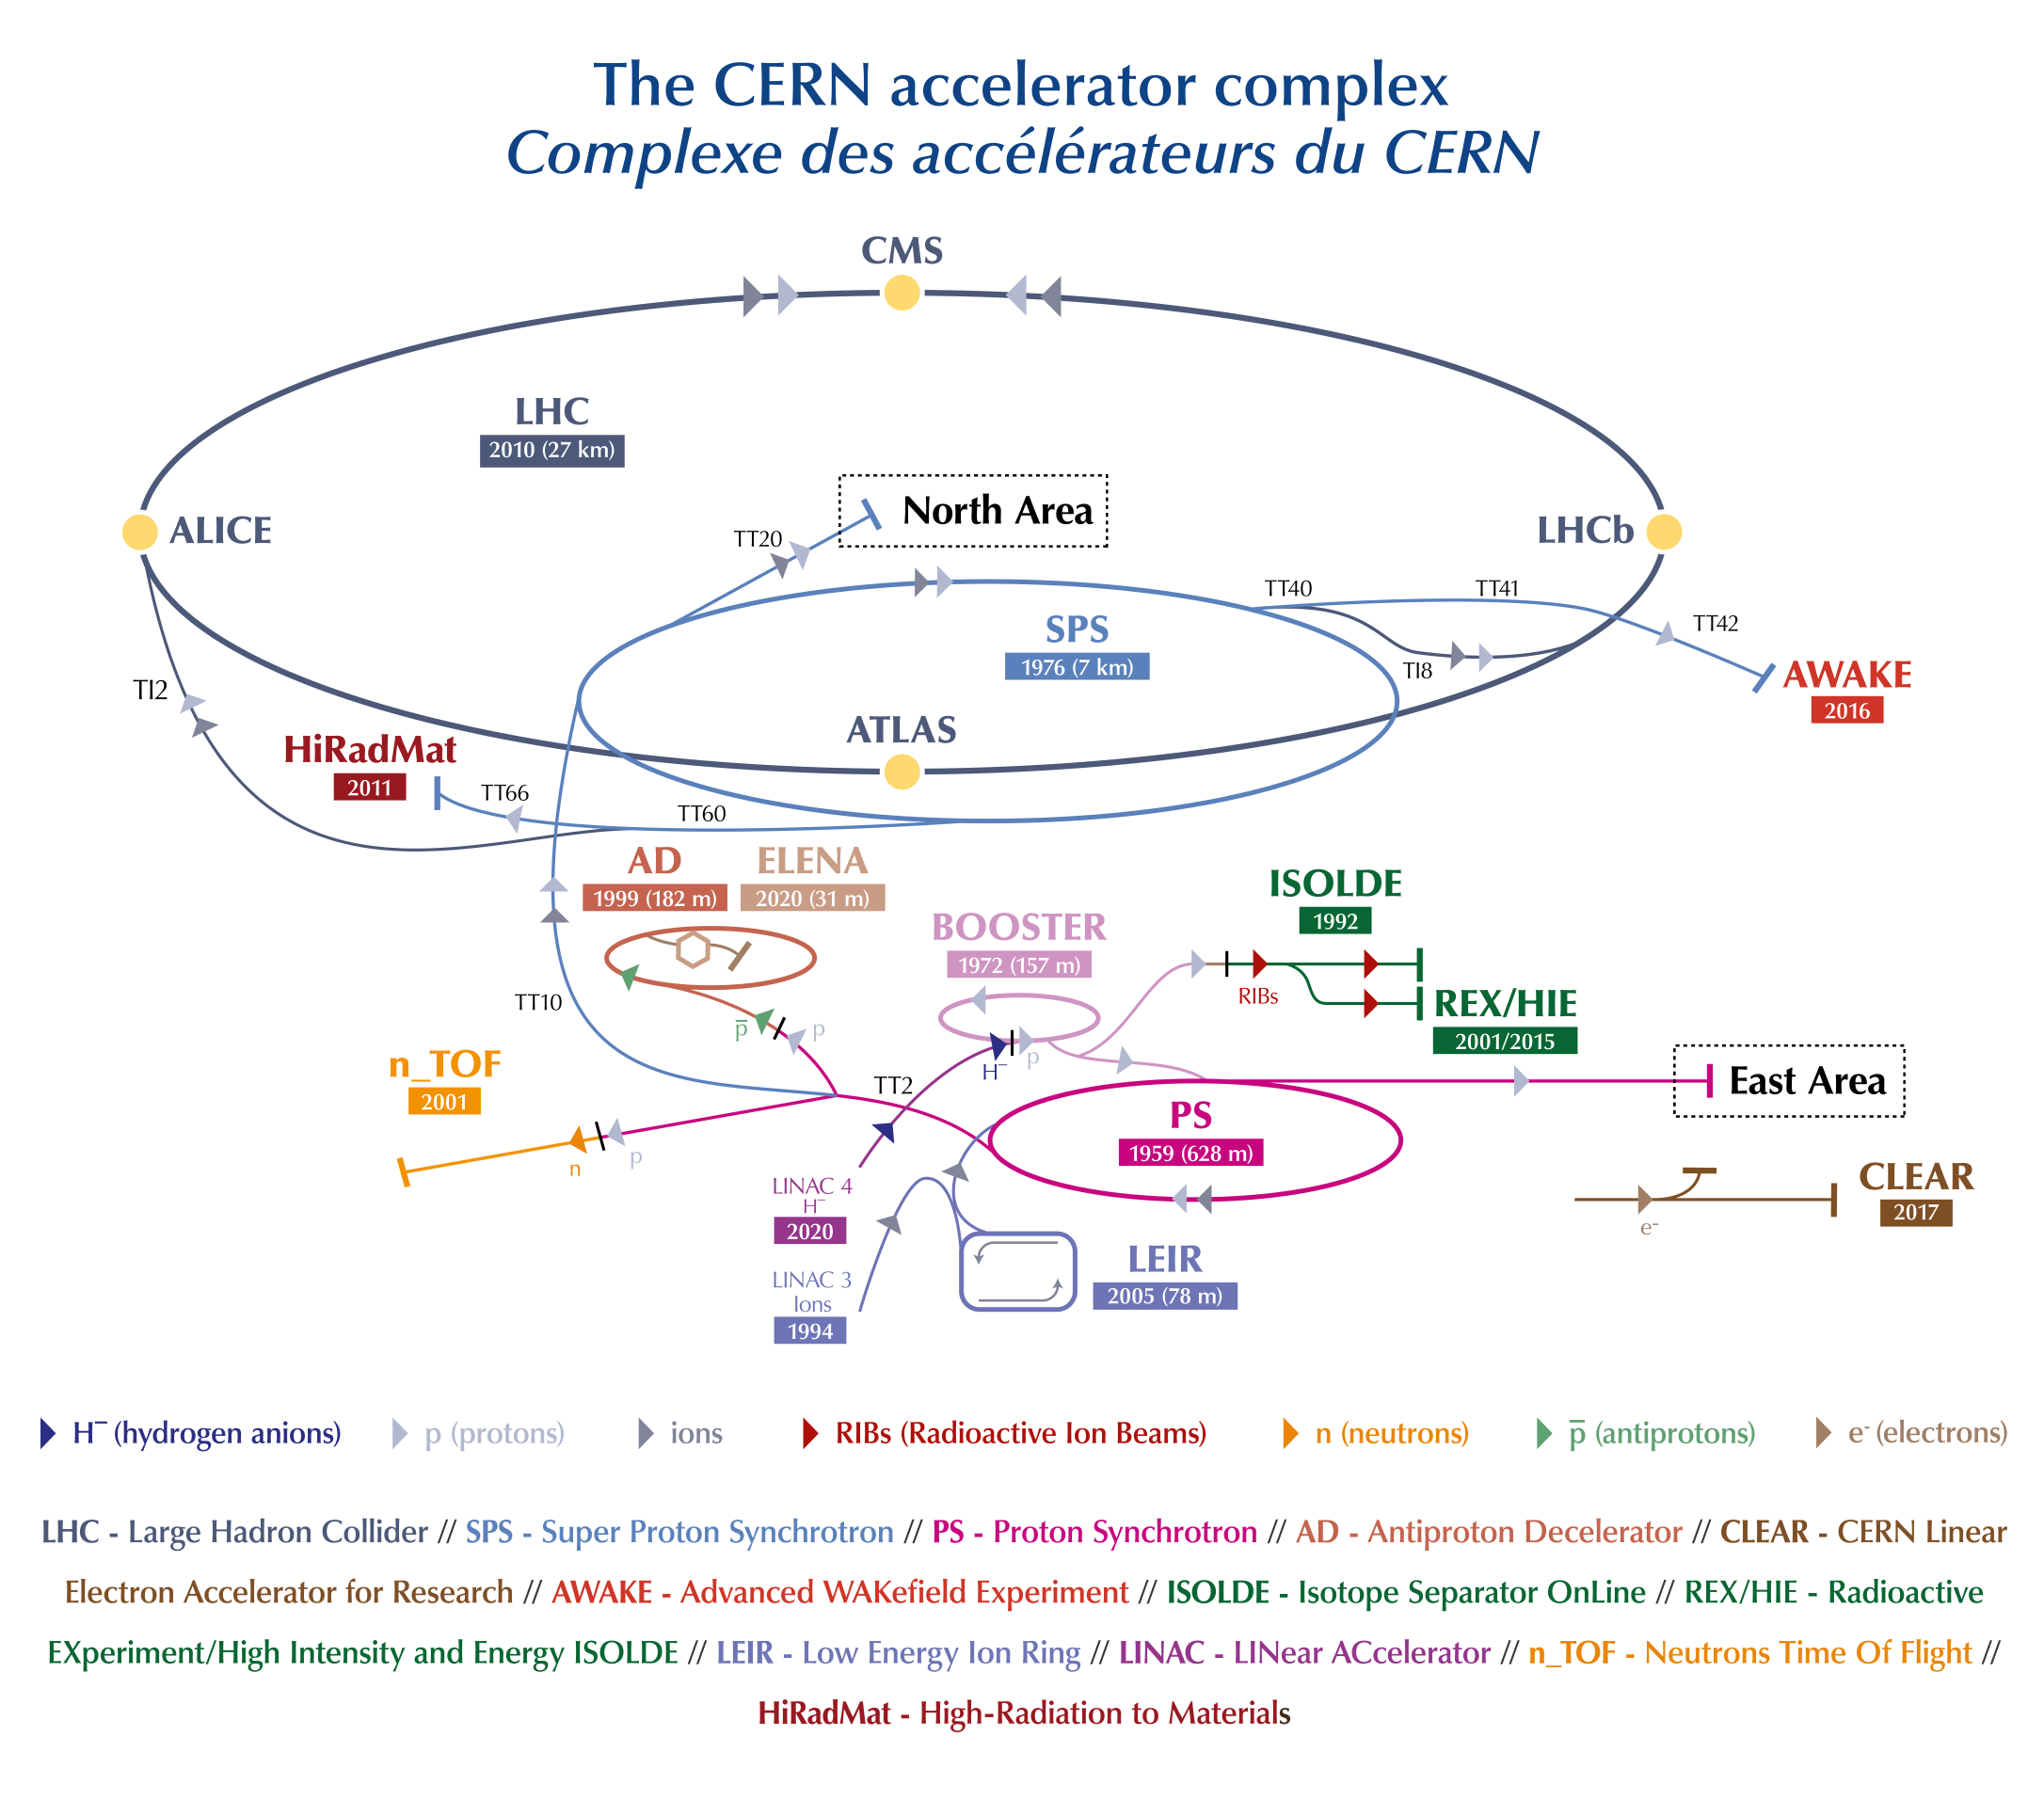
\includegraphics[width=.9\textwidth]{Detector/plots/accelerator_complex_smaller.png}
	\caption{The LHC is the last ring (dark blue line) in a complex chain of 
	particle accelerators. The smaller machines are used in a chain to help boost 
	the particles to their final energies and provide beams to a whole set of smaller experiments.
		}
	\label{fig:accelerator_complex}
	\end{centering}
\end{figure}

The protons are produced by stripping off the electrons from hydrogen gas
in an electric field. Linac 2, the first accelerator in the chain, 
is a linear accelerator which accelerates the protons to an energy of 50~MeV. 
They then enter the PSB, which accelerates the protons to 1.4~GeV, followed by 
the PS, where they reach 25~GeV. The series of radio frequency cavities in 
the PS splits the beam into discrete bunches of protons of 25 ns spacing. 
These bunches are then accelerated to 450~GeV in the SPS, from which they 
are finally injected into the beam pipes of the LHC. 
Each proton beam contains 2808 bunches, arranged in ``trains''
with 72 bunches each ``carriage'' of a gap of around 320 ns between each carriage. 
The beams are required to have well defined transverse and longitudinal emittance. 

The beam pipes are kept at ultra-high vacuum, a vacuum thinner than 
interstellar void, matianed for 24 km of low-temperature section and 3 km 
of room-temperature section. For the low temperature section, the vacuum is 
achieved by pumping in $9000$ m$^3$ of cryogenic gas, which later will be 
condensed and adhered to the surface of the beampipe. 
For the room temperature section, the vacuum 
is achieved by use of non-evaporable getter (NEG) that absorbs residue 
gas particles when heated. More residue is absorbed by an ion pumper. 

The beam pipes are installed in the existing tunnel that was constructed 
between 1984 and 1989 for the Large Electron-Positron Collider (LEP)~\cite{Myers:1991ym}, 
which lies between 45~m and 170~m below the surface on a plane inclined at 1.4\% sloping 
towards the Léman lake.
% Approximately 90\% of its length is in molasse rock, which has excellent 
% characteristics for this application, and 10\% is in limestone under the Jura mountain. 
% There are two transfer tunnels, each approxi-mately 2.5 km in length, linking the 
% LHC to the CERN accelerator complex that acts as injector. 
% These two beams are kept in separate beam pipes,
% cooled to $-271.3^\circ$C ($1.9$ K) with liquid 
% helium distributed by dedicated system, 
%  and ultra-high vacuum, 
There are advantages and disadvantages for a proton-proton collider,
compared to the electron-positron collider like LEP or proton-anti-proton collider.
% The proton-proton collider has advantages 
% and disadvantages compared 
For the LHC, two rings are needed to accommodate the two counter-rotating beams, 
unlike particle-antiparticle colliders that can have both beams sharing the same 
phase space in a single ring, and therefore sharing the same magnets, same radio 
frequency cavities, etc. However, LHC is able to achieve very high collision energy
which is not possible using electron-positron colliders, neither linear nor circular ones.
This is due to the fact that in a circular electron collider, synchrotron radiation lost is 
proportional to the Lorentz factor $\gamma = E/m$ to the power of four, where $E$ and $m$ are
the energy and mass of the particle, respectively. Since electrons are about
2000 times lighter than protons, synchrotron radiation lost is at the order of $10^{13}$
faster for electrons than for protons. For linear electron-positron collider, an extremely long
acceleration section is required with current technologies, which makes it an impractical option.
As for the proton-anti-proton collider, it would not be possible to achieve such 
high luminosity using anti-proton beams, since it is much more difficult 
to produce anti-protons than to produce protons. In addition, at high energies
the proton anti-proton collider starts losing one of its advantages of having higher cross section, 
which is due to the quark sea and anti-quarks in protons become more ``visible'' at high
energies (more details in the parton model section).
% In principle, since the mass of the proton is much larger than 
% the mass of the electron, the
% synchrotron radiation for the losses will be much smaller, and 
% the long straight sections designed to compensate the losses 
% (as designed for the LEP) can be reduced. 
% However these sections are kept 
% as the LEP has as a cost-effective solution, which avoids  
% re-excavating the tunnel. 
% The tunnel in the arcs has a finished internal diameter of 3.7~m. 

As explained above, two separate rings are required to accomodate the two beam pipes, while
the internal diameter of the tunnel is only about 3.8~m. It's technically challenging to 
install them in such small space. LHC therefore adopted the twin-bore magnet design~\cite{rossi2003lhc}, 
as shown in Figure~\ref{fig:double-bore-magnet}. It was first proposed by John Blewett at the Brookhaven 
laboratory in 1971 due to cost considerations~\cite{Blewett:1971zzb}, but in the case 
of the LHC the overriding reason for adopting this solution	is the lack of space in the tunnel. 
\begin{figure}[bht]
	\begin{centering}	
	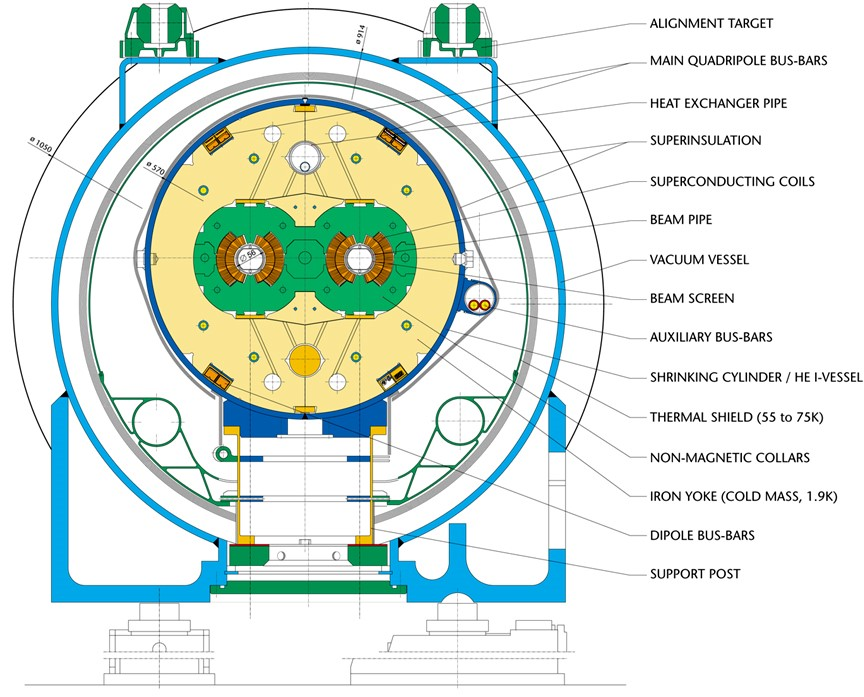
\includegraphics[width=.7\textwidth]{Detector/plots/LHC-double-bore-magnet.jpg}
	\caption{ Double-bore magnet configuration of the LHC 
	superconducting magnets~\cite{rossi2003lhc}.}
	\label{fig:double-bore-magnet}
	\end{centering}
\end{figure}

\subsection{Luminosity and pileup}
\label{sec:LHC:pileup}
% The aim of the LHC is to reveal the physics beyond
% the Standard Model with centre of mass collision energies of up to 14 TeV.
Luminosity is an important measure of a collider's performance.
It comes closely to the number of events generated per second, given by:
\[
	N = \mathcal{L}\sigma,
\]
where $\sigma$ is the scattering cross section 
for the event under study and $\mathcal{L}$ is the machine luminosity. 
For the cross-section, it is more common to use barn as the unit, 
where 1b~=~10$^{-28}$~m$^2$~=~10$^{-24}$~cm$^2$, 
since particle interactions usually have very small cross-sections. 
The machine luminosity depends on the beam parameters 
and can be written for a Gaussian beam distribution as:
\[
	\mathcal{L} = \frac{N_b^2 n_b f_{rev} \gamma_r}{4\pi \epsilon_n \beta*} F,
\]
where $N_b$~refers to the number of protons per bunch,
$n_b$~is number of bunches per beam,
$f_{rev}$~is the revolution frequency, 
$\gamma_r$~is the relativistic gamma factor, 
$\epsilon_r$~is the normalised transverse beam emittance, 
$\beta*$~is the beta function at the collision point which
describes the size of the beam, 
and	$F$ refers to the geometric luminosity reduction factor due to the 
crossing angle at the interaction point. 
While the instantaneous luminosity measures the rate of collisions (per unit cross-section), 
the total number of collisions (per unit cross-section) is measured by the integrated luminosity L, 
given by:
\[
	L = \int \mathcal{L} dt,
\]
which is the integral of the instantaneous luminosity over time.

The two general purpose experiments, ATLAS and CMS are
both aiming at a peak luminosity of $\mathcal{L}$ = $10^{34}$ cm$^2$s$^{-1}$ for proton proton collision,
which corresponds to about one billion $pp$ collisions per second. 
The instantaneous luminosity was much improved at real-time operations reaching about 
twice the nominal (from 2015 to 2018) thanks to the effort of the LHC experts. 

Another important parameter for the LHC experiments is the pileup, 
which is a measure of the number of inelastic $pp$ interactions that occur per bunch crossing. 
Higher pileup gives more luminosity (for a fixed number of bunches) 
but makes physics analysis more difficult due to the signals in the detector 
from the additional interactions. The distribution of the recorded luminosity over
the pileup is shown in Figure~\ref{fig:Run2_pileup} for operations from 2015 to 2018 (Run 2), 
where the <$\mu$> stands for the mean number of interactions per bunch crossing.
There are two main sources of pileup: in-time pileup and out-of-time pileup.
The former refers to the additional proton-proton collisions occuring in
the same bunch-crossing as the collision of interest. 
The later refers to the additional proton-proton collisions occuring
in bunch-crossings just before and after the collision of interest. 
% The out-of-time pileup is a challenge for the detector subsystems that 
% have sensitivity windows longer than
% 25 ns, the interval between bunch crossings.
%  It's a challenging task for the 
% trigger and reconstruction algorithms to achieve robustness under such high pileup 
% condition.
\begin{figure}[bht]
	\begin{centering}	
	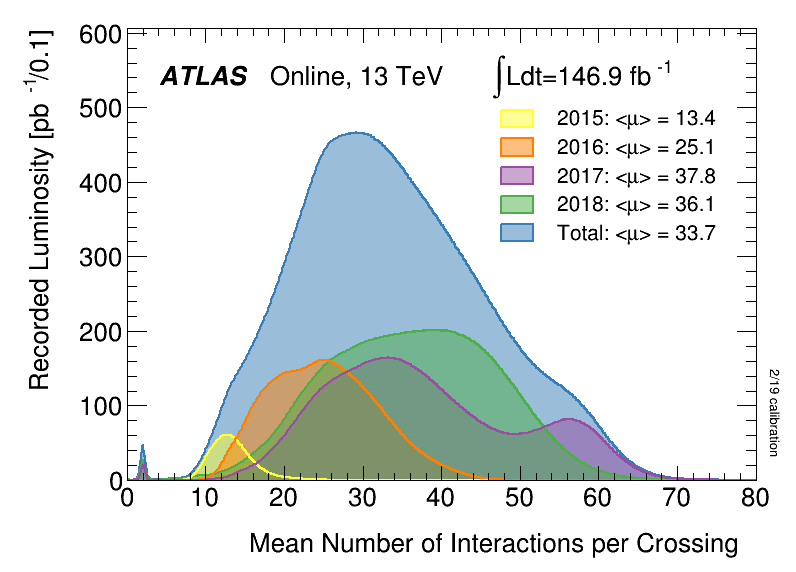
\includegraphics[width=.6\textwidth]{Detector/plots/Run2_pileup.png}
	\caption{Shown is the luminosity-weighted distribution of the mean number of 
	interactions per crossing for the data collected by the ATLAS from 2015 to 2018. 
	All data recorded by ATLAS during stable beams is shown, and the integrated luminosity and 
	the mean $\mu$ value are given in the figure. 
		}
	\label{fig:Run2_pileup}
	\end{centering}
\end{figure}

\subsection{Operation schedule}
\label{sec:Operation schedule}
The LHC operation and shutdown schedule is shown 
% in Figure~\ref{fig:LHC-longterm-schedule}
in Figure~\ref{fig:LHC-schedule-lumi}.
Following the downtime after an incident in one of the main dipole circuits 
during the first commissioning in 2008~\cite{lebrun2009report},
the operation restarted at lower beam energy to minimise the risk. 
Therefore, the first proton run (2010-2013)~\cite{alemany2013operation} was
carried out at 3.5–4 TeV per beam (centre of mass energy 7-8 TeV). 
Furthermore, a bunch spacing of 50 ns was used instead of the nominal 25 ns,
% This implied fewer bunches with larger intensity and hence a 
with peak luminosity of 0.8 $\times$ 10$^{34}$ cm$^{-2}$s$^{-1}$, 
% still smaller than
% the nominal 10$^{34}$ cm$^{-2}$s$^{-1}$ luminosity) 
and pileup larger than nominal. 
% \begin{figure}[bht]
% 	\begin{centering}	
% 	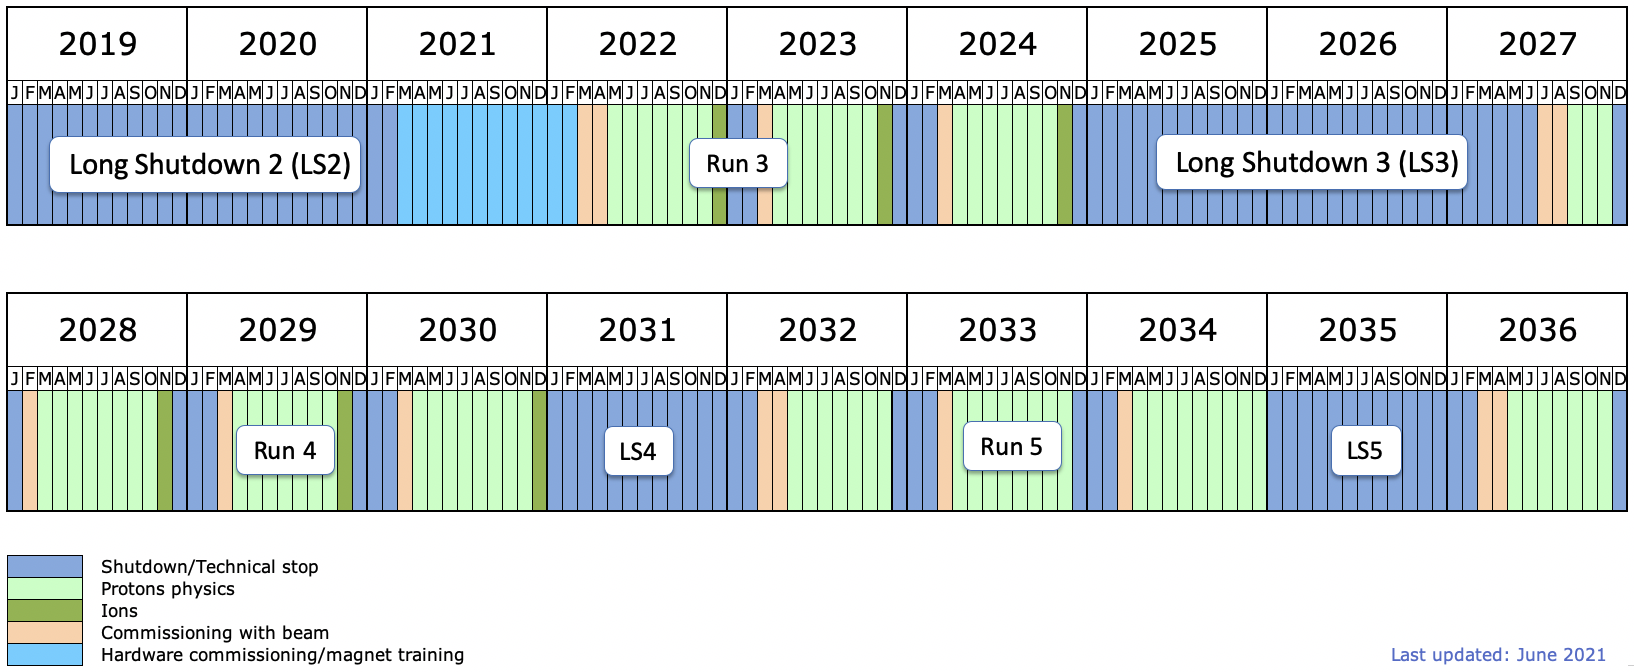
\includegraphics[width=.9\textwidth]{Detector/plots/LHC-longterm-schedule.png}
% 	\caption{Longer term LHC operation schedule.% [source: https://lhc-commissioning.web.cern.ch/schedule/LHC-long-term.htm]
% 		}
% 	\label{fig:LHC-longterm-schedule}
% 	\end{centering}
% \end{figure}

\begin{figure}[bht]
	\begin{centering}
	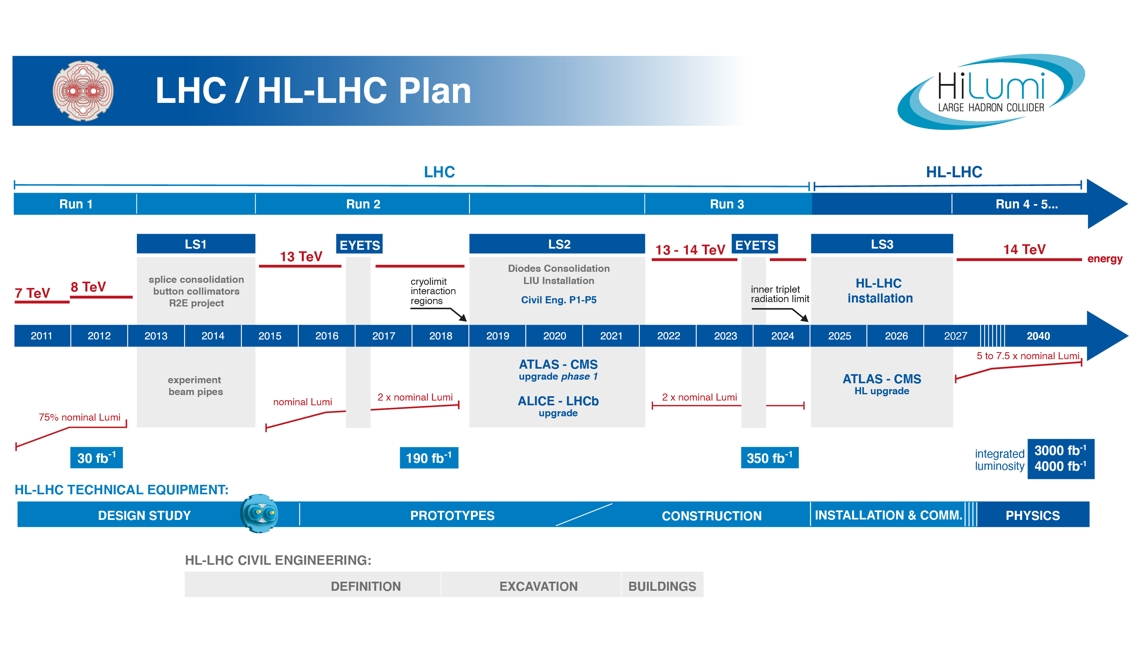
\includegraphics[width=.95\textwidth]{Detector/plots/LHC-schedule-lumi.jpg}
	\caption{LHC operation schedule and luminosity targets.  %[source:project HL-LHC, https://project-hl-lhc-industry.web.cern.ch/content/project-schedule ]
		}
	\label{fig:LHC-schedule-lumi}
	\end{centering}
\end{figure}
In Run 1, the LHC delivered about 30~\fb\ of proton data and important physics results,
most notably the discovery of the Higgs boson~\cite{HIGG-2012-27,HIGG-2012-28}.
Run 1 was followed by a long shutdown (LS1, 2013–2014)
with a large number of consolidation and upgrade activities~\cite{bordry2013first}. 	
The bus-bar splices between the superconducting magnets were improved, 
in order to make sure that the LHC could operate at higher energy 
without risk of repeating the 2008 incident. 

\begin{figure}[bht]
	\begin{centering}	
	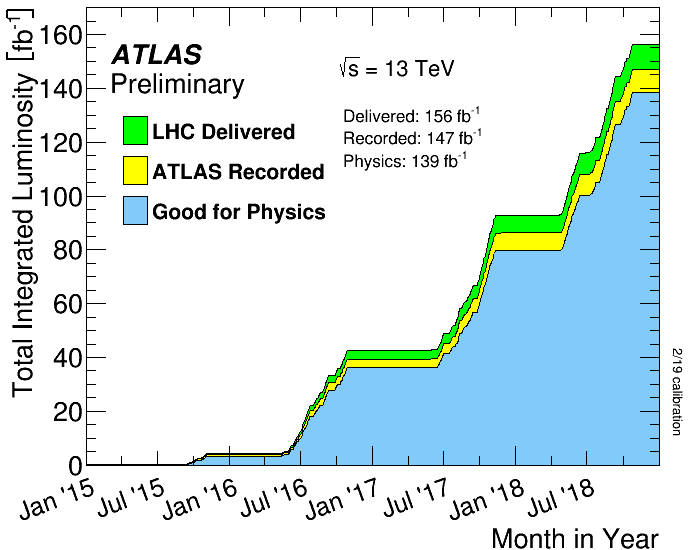
\includegraphics[width=.6\textwidth]{Detector/plots/Run2_lumi.png}
	\caption{Cumulative luminosity versus time delivered to 
	ATLAS (green), recorded by ATLAS (yellow), and certified to be 
	good quality data (blue) during stable beams for $pp$ collisions 
	at 13 TeV centre-of-mass energy in Run 2. 
		}
	\label{fig:Run2_lumi}
	\end{centering}
\end{figure}

Run 2 (2016-2018) was carried out
at 6.5 TeV per beam (center of mass energy 13 TeV)~\cite{LHC-Run2-Operation}. 
As shown in Figure~\ref{fig:Run2_lumi}, out of the 156~\fb\ 
of data LHC has delivered at 13 TeV centre of mass energy, the ATLAS detector has recorded 
147~\fb\ and \lumi\ of data is certified to be good quality data.
The 156~\fb\ data accounts for the luminosity delivered from the start of 
stable beams until the LHC requests ATLAS to put the detector in a 
safe standby mode to allow a beam dump or beam studies. 
The recorded luminosity is slightly smaller than the delivered luminosity, due 
to the inefficiency of the Data Acquisition and the so called ``warm start'': 
when the stable beam flag is raised, 
the tracking detectors undergo a ramp of the high-voltage and, 
for the pixel system, turning on the pre-amplifiers. 
More details of the ATLAS detector can be found in the following sections. 
The recorded data is checked carefully to exclude possible hardware or software  issues. 
This is achieved by monitoring detector-level quantities 
and reconstructed collision event characteristics at key stages of the data processing chain.
This procedure led to high efficiency of good quality data: 95.6\%~\cite{aad2020atlas}.	

In this thesis the \lumi\ data recorded by the ATLAS detector of Run 2 is used.
The nominal bunch spacing of 25 ns was used, with slightly less bunches (2500) per beam.
The LHC experts have continually improved the running scenario to increase the luminosity,
and during Run 2 the luminosity surpassed the designed luminosity by a factor of 2. 
As well as improving the instantaneous luminosity, the availability of the machine
was dramatically improved during Run 2 which is an important factor enabling the high efficiency 
of good quality data as mentioned above.
During Run 2, the machine was providing physics collisions during 50\% of 
the allocated physics time, which is very impressive for a super conducting collider. 

The operation of CERN’s accelerators is subject to scheduled shutdowns 
to allow important repair and upgrade work to take place. 
The present shutdown, LS2, is devoted to preparations for Run 3 of the LHC, 
which will have an integrated luminosity equal to the two previous runs combined, 
and for the High-Luminosity LHC (HL-LHC), 
the successor to the LHC, which will begin operation at the end of 2027,
and eventually generate 10 times the integrated luminosity of
all Run 1, 2 and 3 combined!

The LS2 schedule has had to be modified due to the COVID-19 pandemic, 
which the new schedule anticipates that the first test beams will 
circulate in the LHC 
at the end of September 2021, four months later than the date 
planned before the COVID-19 crisis, 
to give the LHC’s main experiments – ATLAS, CMS, ALICE and LHCb – 
time to prepare their own upgrade. 
Run 3 of the LHC will begin at the start of March 2022.
% No changes have been made to the schedule beyond 2022.
The third long shutdown (LS3) will begin at the 
start of 2025 and end in mid-2027. 
This is when the equipment for the HL-LHC and 
its experiments will be installed. 

\section{The ATLAS Detector}

ATLAS is one of the two general purpose detectors built for probing proton-proton 
collision. This detector represents the work of a large collaboration 
of several thousand physicists, engineers, technicians,
and students over a period of fifteen years of dedicated 
design, development, fabrication, and installation.
The overall layout of the detector is shown in Figure~\ref{fig:ATLAS_cut_away}~\cite{PERF-2007-01}.
It has the shape of a cylinder, 46~m long, 25~m in diameter, 
and sits in a cavern 100~m below ground. The ATLAS detector weighs 7000 tonnes, 
similar to the weight of the Eiffel Tower.
The detector itself is a many-layered instrument designed to detect some 
of most energetic particles ever created on earth. 
It consists of six different detecting subsystems wrapped concentrically 
in layers around the collision point of nearly 4$\pi$ solid angle coverage
to record the trajectory, momentum, and energy of particles, 
allowing them to be individually identified and measured. 
These six subsystems are 
the pixel detector~\cite{ATLAS-TDR-11}, 
the semiconductor tracker (SCT)~\cite{ATLAS-TDR-04}, 
the transition radiation tracker (TRT)~\cite{ATLAS-TDR-04},
the electromagnetic (EM) calorimeter~\cite{ATLAS-TDR-02}, 
the hadronic calorimeter~\cite{ATLAS-TDR-03}
and the muon spectrometer (MS)~\cite{ATLAS-TDR-10}.
The first three sub-detectors are collectively known as the inner detector (ID),
described in section~\ref{sec:inner detector}, and it is used for tracking charged particles. 
The electromagnetic and the hadronic calorimeter, described in section~\ref{sec:calorimeter},
are responsible for measuring the energies of the electromagnetic and hadronic particles respectively. 
The MS, described in section~\ref{sec:MS}, is a unique sub-detector used for measuring the 
momentum of muons leaving the calorimeters.

A huge magnet system bends the paths of the charged particles so that their 
momenta can be measured as precisely as possible.

\begin{figure}[bht]
\begin{centering}	
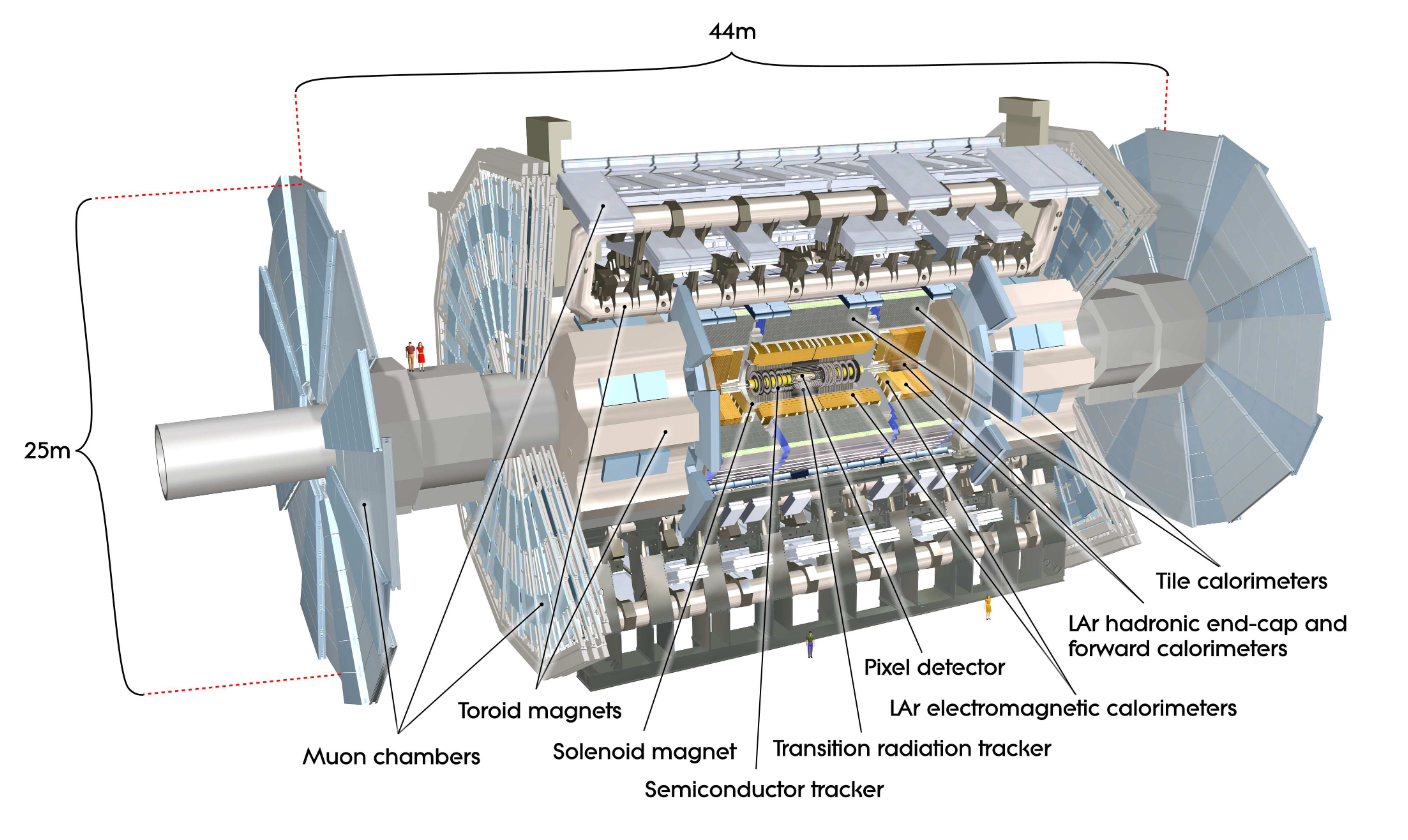
\includegraphics[width=1.0\textwidth]{Detector/plots/Cut-away-view-of-the-ATLAS-detector.png}
\caption{Cut-away view of the ATLAS detector. 
The dimensions of the detector are 25~m in
height and 44~m in length. The overall weight 
of the detector is approximately 7000 tonnes. The figure is taken from reference \cite{PERF-2007-01}.
	}
\label{fig:ATLAS_cut_away}
\end{centering}
\end{figure}

The high interaction rates, radiation doses, particle multiplicities 
and energies, as well as the requirements for precision measurements 
have set strigent standards on the design of the ATLAS detector. 
Therefore the ATLAS detector is designed to fufiled the following 
requirements:

\begin{itemize}
\item
Fast, radiation-resistant electronics and sensor elements 
and high detector granularity. This is due to the
 high frequency of collisions, high particle fluxes and 
 high radiation environment of the detector.
\item
Large acceptance in polar angle with almost full azimuthal angle coverage,
due to the geometry of the detector 
(more details in section~\ref{sec:detector coordinate}).
\item
Good energy resolution calorimetry, as required to 
enable accurate physical object reconstruction. 
The high resolution of energy can be obtained 
with very good electromagnetic calorimetry for 
electron and photon identification and measurements,
complemented by full-coverage hadronic calorimetry 
for accurate jet and missing transverse energy measurements.
\item  
Tracking of precision in the ID, as required to provide high momentum 
resolution and to allow the reconstruction of
secondary vertices to identify $b$-hadrons and $\tau$-leptons.
\item
Good muon identification and momentum resolution 
over a wide range of momenta and the ability 
to determine unambiguously the charge of high-\pt\ 
muons in the muon spectrometer.
\item
Trigger system with high efficiency on low \pt\  
objects with sufficient background rejection, 
which is a prerequisite to achieve an acceptable trigger rate 
for most physics processes of interest.
\end{itemize}


The main performance goals of the detector are 
listed in Table \ref{tab:ATLAS_performance}. 
\begin{table}[thb]
	\centering
	\small
	\setlength\tabcolsep{5pt} 
	\begin{tabular}{|l|l|l|l| }
	\hline
	\multirow{2}{*}{Detector component}&\multirow{2}{*}{Required resolution} & \multicolumn{2}{l|}{$\eta$ coverage} \\ \cline{3-4}
	
	  & & Measurement &  Trigger\\ 
	 \hline
	Tracking         &    $\sigma_{p_T}/p_T = 0.05\%\ p_T\bigoplus 1\% $        &  $\pm 2.5$  & None \\  
	\hline
	EM calorimetry      &  $\sigma_E/E = 10\%\ /E\bigoplus 0.7\% $       & $\pm 3.2$ &  $\pm 2.5$\\
	\hline
	Hadronic calorimetry  &        & &      \\
	% \hline
	\ \ barrel and end-cap &  $\sigma_E/E = 50\%/E\bigoplus 3\% $       & $\pm 3.2$ &  $\pm 3.2$\\
	\ \ forward   &  $\sigma_E/E = 100\%\ /E\bigoplus 10\% $       & $ 3.1 < |\eta | < 4.9 $ &  $3.1 < |\eta | < 4.9 $\\
	\hline
	Muon spectrometer  &    $\sigma_{p_T}/p_T = 10\%$ at \pt $=\ 1$ TeV        &  $\pm 2.7$  & $\pm 2.4$ \\  
	\hline
	\end{tabular}
	\vspace{0.2cm}
	\caption{General performance goals of the ATLAS detector. The units for energy of the particle, E
	and transverse momentum, \pt\ (detailed definition in section~\ref{sec:detector coordinate}) 
	are in GeV~\cite{PERF-2007-01}. Note that, for high-\pt\ muons,
	the muon-spectrometer performance is independent of the inner-detector system.}
	\label{tab:ATLAS_performance}
\end{table}



\subsection{Coordinate system}
\label{sec:detector coordinate}

The ATLAS coordinate system is a right-handed Cartesian system
with the nominal interaction point 
defined as the origin of the coordinate system,  
while the beam direction defines the $z$-axis and 
the $x$-$y$ plane is transverse to the beam direction.  
The positive $x$-axis is defined as pointing from 
the interaction point to the centre of the
LHC ring and the positive $y$-axis is defined as 
pointing upwards, as shown in Figure~\ref{fig:ATLAS_coordinate_system}. 

\begin{figure}[bht]
	\begin{centering}	
	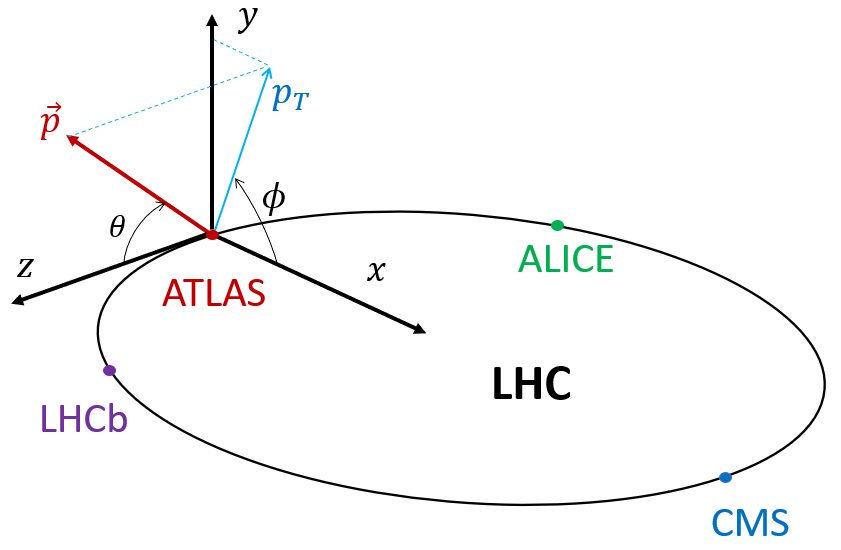
\includegraphics[width=.75\textwidth]{Detector/plots/ATLAS coordinate system.png}
	\caption{Illustration of the coordinate system
	used at the ATLAS experiment in the geographical context of the LHC.
		}
	\label{fig:ATLAS_coordinate_system}
	\end{centering}
\end{figure}

The azimuthal angle $\phi$ 	is measured as usual around the beam axis, 
and the polar angle $\theta$ is the angle from the beam axis.  
In high energy physics, it's more common to use the 
pseudorapidity instead of the polar angle $\theta$, defined as:
\[
		\eta = -\ln\ \tan(\theta/2). 
\]
In the case of highly relativistic particles
(which is the comman case in high energy physics), 
the pseudorapidity approaches the rapidity, 
\[ 
	y=1/2\ln[(E+p_z)/(E-p_z)], 
\]
where $E$ is the energy of the particle, $m$ is its mass 
and $p_z$ is the momentum along the $z$-axis.
There are two main reasons for using pseudorapidity 
rather than the polar angle $\theta$ nor the rapidity.
The reason for using pseudorapidity but not $\theta$ 
is that the rapidity is invariant
under Lorentz transformation, while capturing 
the characteristic of the particle direction of travel:
$y \rightarrow \pm \infty $ when the particle is  
travelling close to the beam pipe (positive for along the
beam pipe, negative for the opposite direction) and
$y \rightarrow 0$ when $p_z$ is small.
The reason for using pseudorapidity but not rapidity
is that due to the limited angle coverage of the detector, 
it's usually hard to determine the total energy and the momentum 
along the $z$-axis, especially when the direction of 
the particles are close to the beam pipe. 
While the pseudorapidity is determined only by
the polar angle, which is much easier and faster 
to compute. 
Another commonly used variable, transverse momentum \pt, 
is defined as the momentum of a particle transverse to the 
beam direction ($z$-direction):
\[ 
	\vec{p_T}= (p_x,p_y).
\]
The reason for using transverse momentum 
is that, because the partons that make up a proton share the momentum,
the initial longitudinal momentum is unknown;	
we do know, however, that the initial transverse momentum was zero. 
And hence we can look for the missing transverse momentum, defined
as 
\[ 
	\vec{E_T}^{miss}=-\sum_i \vec{p_{T_i}} \label{eq:MET}
\]
for visible particles $i$, where \met\ is the magnitude of $\vec{E_T}^{miss}$
 (Confusingly $E_T^{miss}$ is commonly called 
missing transverse energy or MET. Missing transverse energy is equivalent 
to missing transverse momentum only if the missing particle(s) were massless.). 
Finnaly, the distance $\Delta R$ in the pseudorapidity-azimuthal angle 
space is defined as:
\[\Delta R = \sqrt{\Delta \eta^2+\Delta\phi^2},\]
where $R$ is the radial distance from the particle position to the interaction 
vertex.

\subsection{Magnets}


ATLAS has a unique hybrid system of four large superconducting 
magnets~\cite{ATLAS-TDR-06}. This magnetic system is 22~m in diameter and 26~m in length, 
with a stored energy of 1.6~GJ. Figure~\ref{fig:ATLAS_magnets_site} shows the real scale of
the magnets system compared to a person. 
Figure~\ref{fig:ATLAS_cut_away} shows the general layout, 
the four main layers of detetors and the four superconducting 
magnets which provide the magnetic
field over a volume of approximately 12000~m$^3$.



\begin{figure}[bht]
	\begin{centering}	
	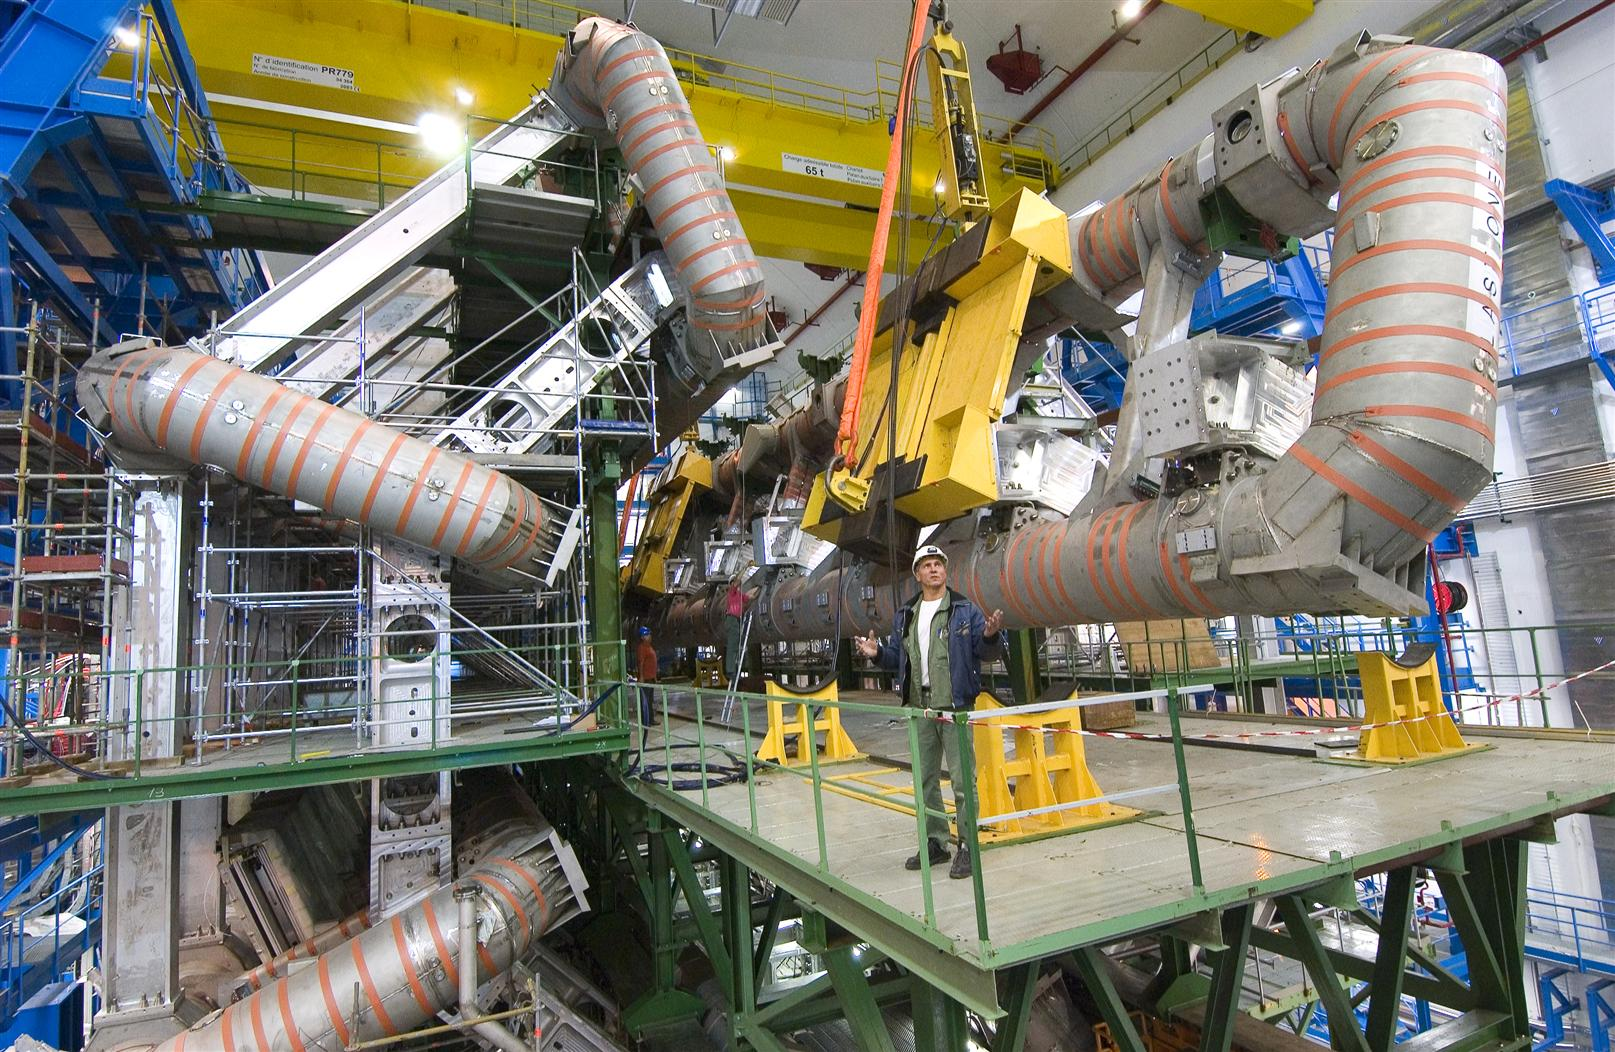
\includegraphics[width=.8\textwidth]{Detector/plots/magnets.jpg}
	\caption{A picture showing the real size magnets compared to a person.}
	\label{fig:ATLAS_magnets_site}
	\end{centering}
\end{figure}




The spatial arrangement of the coil windings is shown in 
Figure~\ref{fig:ATLAS_magnets}. 
The ATLAS magnet system consists of two parts:
\begin{itemize}
	\item a solenoid, which is aligned on the beam axis and 
	provides a 2 T axial magnetic field in the $z$-direction
	for the ID. Becasue the magnet is located in front
	of the EM calorimeter, it is imperative to minimise possible interactions
	between the magnet and the particles being studied.
	This is achieved by embedding over 9 km of niobium-titanium 
	superconductor wires into strengthened, pure aluminum strips, 
	which is capable to provide such powerful magnetic field
	in just 4.5 cm thickness. 
	% while minimising the radiative thickness in front of the	barrel 
	% electromagnetic calorimeter;
	\item  A barrel toroid and two end-cap toroids, 
	which produce a	toroidal magnetic field of approximately 
	0.5 T and 1 T for the muon detectors in the central 
	and end-cap regions, respectively. 
	The barrel toroid generates the magnetic field in the central zone 
	of the muon spectrometer, along the tangential direction of 
	the circumferences centered on the $z$-axis ($\phi$ direction). 
	The end-cap toroids are two smaller toroids designed to 
	provide the magnetic field in the forward areas of 
	the muon spectrometer. 
	This magnet configuration provides a field is mostly orthogonal 
	to the muon trajectories. 
	
\end{itemize}		



\begin{figure}[bht]
	\begin{centering}	
	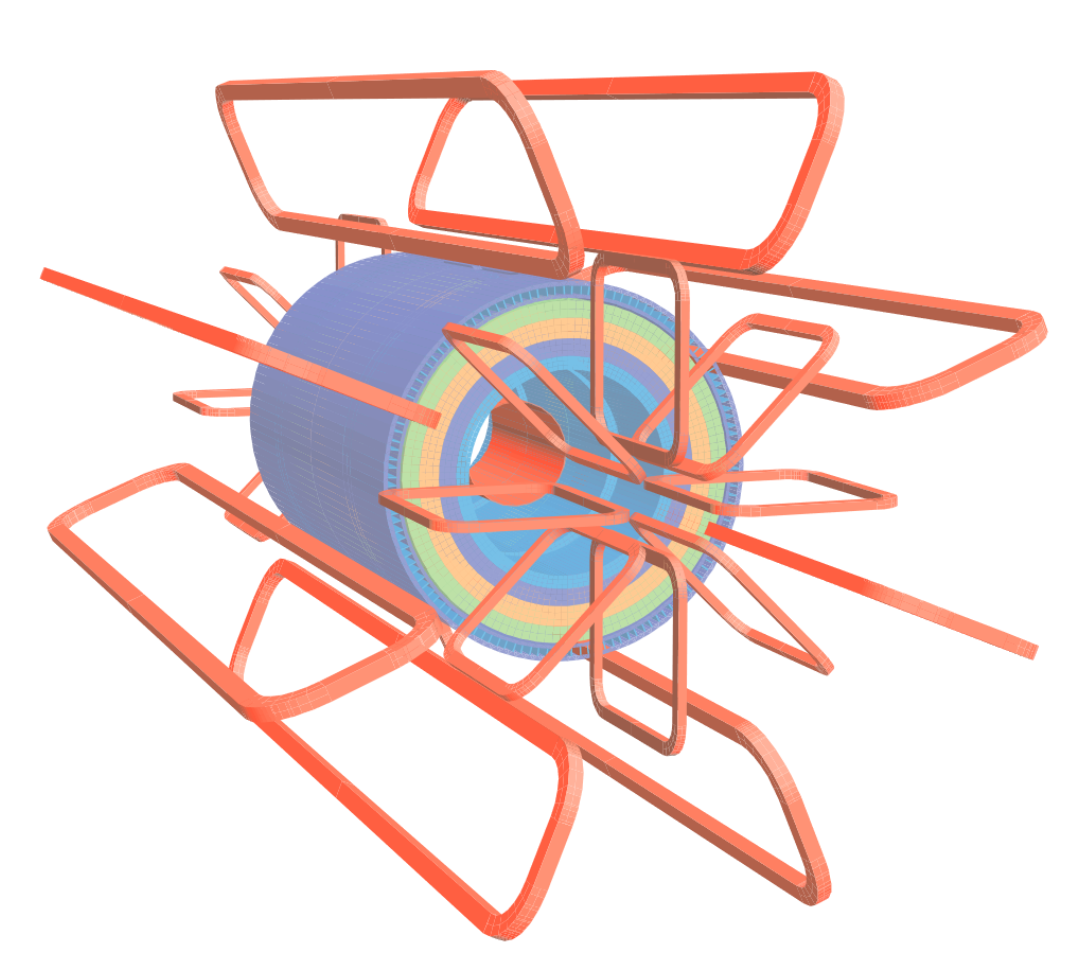
\includegraphics[width=.56\textwidth]{Detector/plots/ATLAS magnets.png}
	\caption{Geometry of magnet windings and
	tile calorimeter steel. Image taken from \cite{PERF-2007-01}.}
	\label{fig:ATLAS_magnets}
	\end{centering}
\end{figure}


\subsection{Inner detector}	
\label{sec:inner detector}
The inner detector (ID) is the closest sub-detector to the
beam line, designed to track the early trajectories of charged particles for
momentum calulations and locat their primary and secondary vertices with
extremely high precision. The ID is required to deal with large numbers of tracks
promptly, where 1000 particle collisions are taking place every 25 ns.  
The ID has full coverage in azimuthal angle $\phi$ and $|\eta|$ < 2.5 acceptance 
in pseudorapidity. As mentioned briefly above, it consists of three parts: 
the pixel detector and the insertable B-Layer (IBL)~\cite{ATLAS-TDR-19} (as one part),
the semiconductor tracker and the transition radiation
tracker. The layout of the ID is shown in figure~\ref{fig:inner_detector},
with a charge track (in red) traversing the sensors and structural elements. 
\begin{figure}[bht]
	\begin{centering}	
	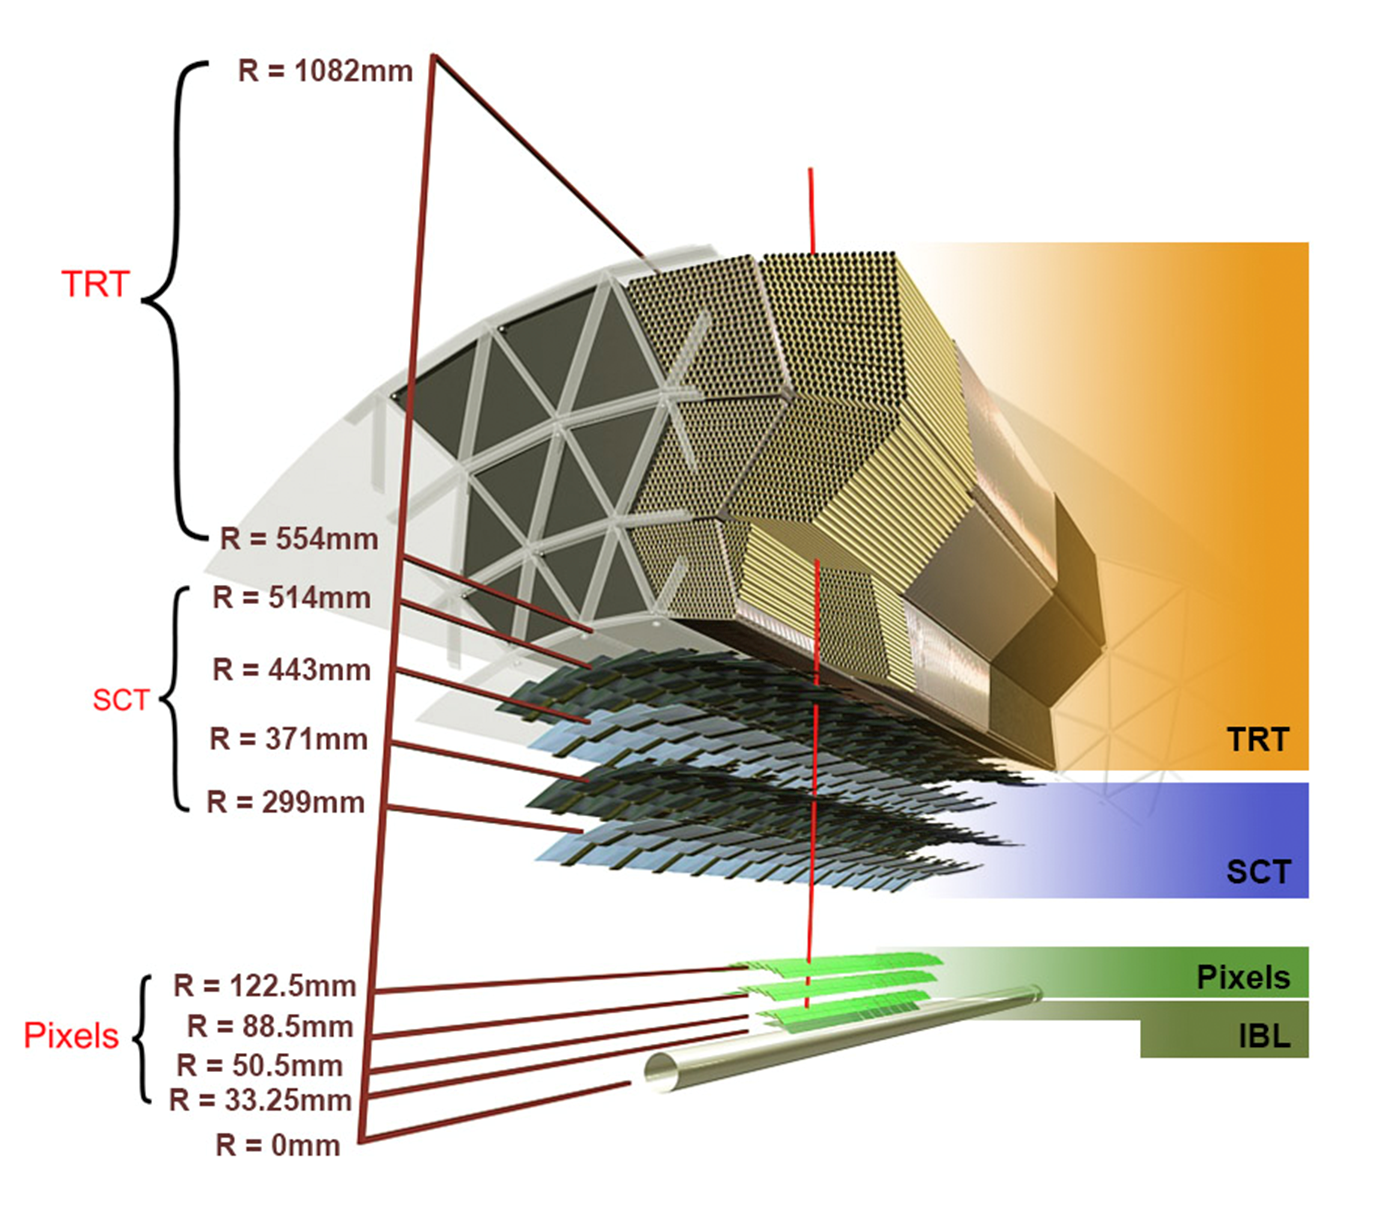
\includegraphics[width=.85\textwidth]{Detector/plots/Inner detector.png}
	\caption{Cut-away view of the inner detector. Image taken from \cite{Pequenao}.}
	\label{fig:inner_detector}
\end{centering}
\end{figure}
% The track traverses successively the beryllium
% beam-pipe, the four cylindrical silicon-pixel layers 
% with individual 
% sensor elements of 50$\times$400 $\mu m^2$, the four cylindrical double 
% layers of barrel SCT of pitch 80 $\mu m$, 
% and approximately 36 axial straws of 4 $mm$ diameter 
% contained in the barrel TRT
% modules within their support structure.
% \begin{itemize}
	\subsubsection{Pixel detector and IBL}
	The silicon pixel detector is the closest ATLAS 
	component to the collision. It is composed of layers of
	silicon pixels and designed to have a very 
	high granularity for reconstructing primary 
	and secondary interaction vertices. 
	The detector layers are formed of silicon sensor modules and 
	in total there are approximately 92~million pixels 
	(consequently, 92~million readout channels) in the system.
	It consists of three cylindrical layers in the 
	barrel region, positioned at the radial distances of 
	50.5, 88.5 and 122.5~mm, 
	and of disks perpendicular to the beams in the end-caps at the
	longitudinal distances of 49.5, 58.0 and 65.0~mm. 
	% The B-layer, placed at a distance of 50.5mm, plays 
	% an important role in detecting secondary vertices 
	% for the identification of jets coming from 
	% b-quark hadronisation (\bjets). 
	In 2014, during the first LHC long shutdown, a fourth pixel 
	layer was installed inside the existing detector, 
	the insertable B-Layer (IBL) at a radius of 33~mm 
	from the beam axis.
	The new pixel layer provides an 
	additional space point very close to the interaction point, 
	which significantly improves the identification of jets coming from 
	$b$-quark hadronisation (\bjets). 
	Particles with $|\eta|$ < 2.5 traverses the four layers usually produce  
	four space-points. The pixel detector provides a resolution of 
	$\sigma_\phi$ = 10 $\mu$m in the bending direction ($R - \phi$), 
	and a resolution of $\sigma$ = 115 $\mu$m in the $z$($R$)
	direction in the barrel (end-cap) region.

	\subsubsection{Semiconductor tracker}
	The next constituent of the inner detector is the SCT. 
	It is a silicon microstrip detector with over six million readout channels, 
	which surrounds the pixel detector and covers the region 
	of radius between 299~mm and 560~mm. 
	It consists of four layers of strips located axially on the 
	beam direction in the barrel region and placed along the 
	$z$-direction in the end-cap region. 
	This configuration allows the particles along the beam pipe
	to be constructed. 
	Each layer of strips is glued back to back with an angle of
	40~mrad to form a two-sided module and make possible the 
	measurement of the second coordinate.
	The sensors are 285 $\mu$m thick and are constructed
	of high-resistivity n-type bulk silicon with p-type implants. 
	Readout strips are positioned every 80 $\mu$m, providing a spatial resolution 
	of $\sigma_\phi = 17\ \mu m$ in the bending direction ($R-\phi$)
	and $\sigma_\phi = 580\ \mu m$ in the z (barrel) and R (end-cap) direction. 

	\subsubsection{Transition radiation tracker}
	The outermost part of the inner detector is the TRT, which covers
	the radial region between 563~mm and 1066~mm. 
	It is a straw drift tube tracker, which consists of
	modules of 4~mm diameter polyimide straws, filled with a mixture of gas of
	70\% Xe, 27\% CO$_2$ and 3\% O$_2$ 
	and a gold-plated tungsten wire in the centre. 
	The straws are interleaved with propylene fibres (foils) in the barrel (end-cap)
	region.
	% All charged tracks with \pt\ $> 0.5$ GeV and $|\eta| < 2.0$ will traverse 
	% at least 36 straws, except in the
	% barrel-end-cap transition region ($0.8 < |\eta|< 1.0$), 
	% where this number decreases to a minimum of 22 crossed straw.
	With a spatial resolution of $\sigma_\phi = 130$ \textrm{$\mu$m}, 
	the TRT measures the track position only in the bending direction
	($R-\phi$). This is because when
	a charged particle passes through a straw tube, electrons from the gas
	are liberated through ionisation; under high voltage, these electrons then drift toward the 
	wire in the certre, where a current flow is created and registered as a hit.
	Since a hit can happen on any location along the wire,
	the information of the $z$ position of the particle is lost. 
	In addition, the TRT provides capability of distinguishing electrons from other
	charged particles. When a highly-relativistic charged particle traverses the
	polymer straws interfacce, the particle emits transition radiation which is then absorbed 
	by the Xeon gas. The intensity of the radiation
	depends on the gamma factor of the particle (strongest for lighter particles), hence this information
	can be exploited for electron identification. 
	% by the particle 
	% The ionisation probability depends on the gamma factor of the charged particle 
	% and hence 
	% The TRT contributes significantly to the pattern recognition and 
	% momentum reconstruction, depsite the low resolution compared to the 
	% silicon tracker and the lack of a measurement along the $z$-axis. 
	% This is the result of the large number of measurements and longer
	% measured track length. In addition, the TRT provides extra ability to 
	% identify elecctrons due to the polypropylene fibres (foils) in the barrel
	% (end-cap) emit photons when a charged particle traverses the boundaries of
	% the material. These photons are then absorbed by the Xenon gas mixture, which
	% the intensity depends on gamma factor of the traversing particle. 
	% This information can then be exploited for electron/pion discrimination.
	% \end{itemize}

\subsection{Calorimeter system}

\label{sec:calorimeter}


Calorimeters are used to measure the energy of both charged and neutral particles. 
The ATLAS calorimeters~\cite{ATLAS-TDR-01}, as shown in Figure~\ref{fig:calo},
are consists of three major components,
the Electromagnetic calorimeter, the Hadronic calorimeter and the Forward calorimeter (FCal).
The fine granularity of the EM calorimeter 
is ideal for precision measurements of electrons and photonsl; the
coarser granularity of hadronic calorimeter is sufficient 
for the hadronic jet reconstruction; the FCal provides coverage of 
large pseudorapidity region: these calorimeters cover the range $|\eta|$< 4.9.
All the three calorimeters are sampling calorimeters. Sampling calorimeters 
use different material the absorber and the active part:
the absorber (or passive material) is reponsible for producing particle showers where 
the active part then measures their energy. Note well the a fraction of
total particles energy deposited in the passive material and it's not
measured; the overall energy must be deduced from the definite
measurements taken in the active detector layers. 

\begin{figure}[bht]
	\begin{centering}	
	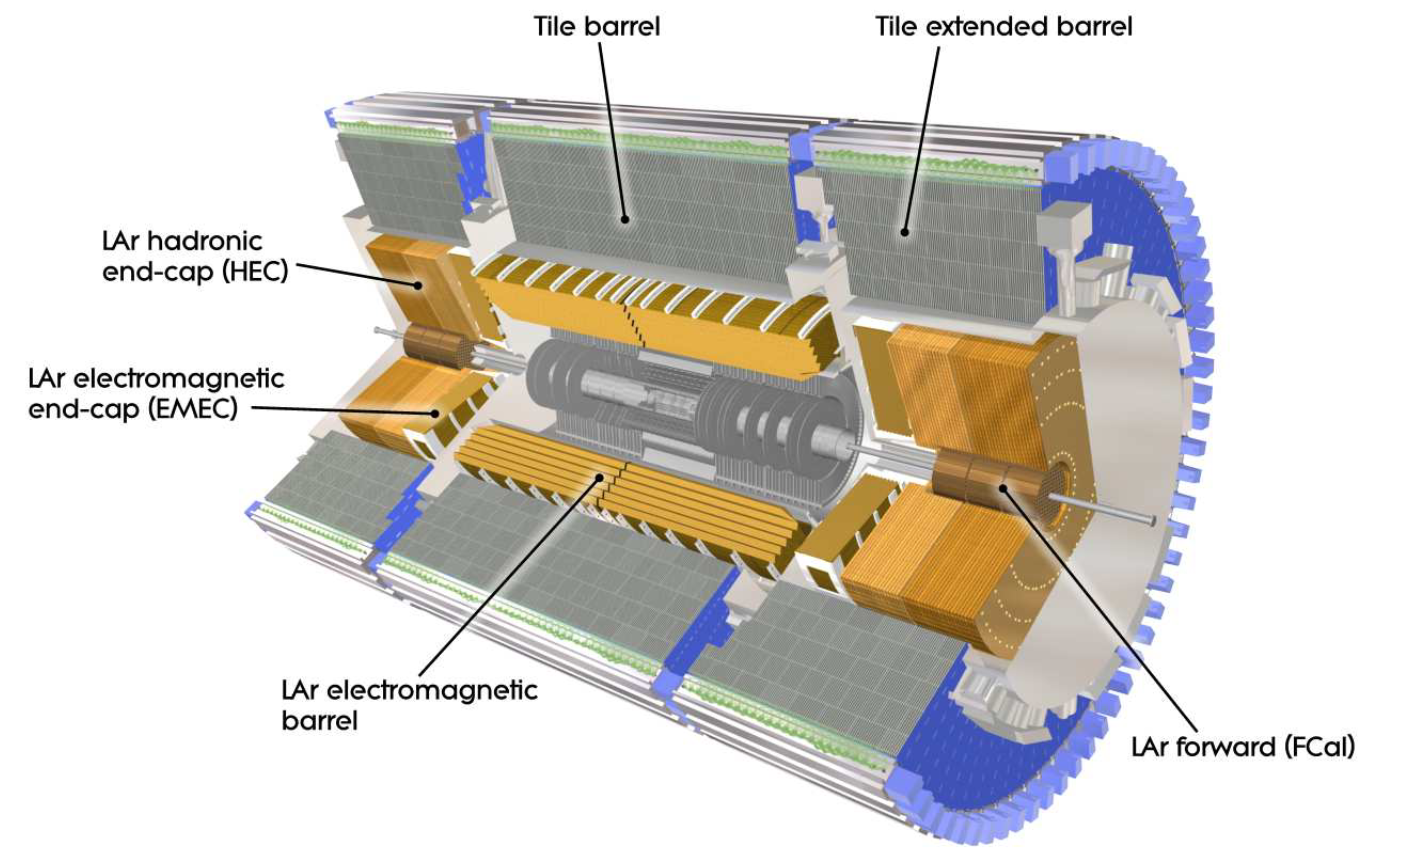
\includegraphics[width=1.0\textwidth]{Detector/plots/calo.png}
	\caption{Cut-away view of the ATLAS calorimeter system. Image taken from~\cite{ATLAS-TDR-01}.}
	\label{fig:calo}
	\end{centering}
\end{figure}
% using different techniques suited to the widely varying requirements 
% of the physics processes of interest and of the radiation environment
% over this large $\eta$-range. 
% over the large $\eta$ region, 
The electromagnetic and hadronic showers must be contained in the 
calorimeter to ensure precise measurement of the total energy of the particle
and to avoid punch-through into the muon system. 
The calorimeter depth is hence an important design consideration. 
The thickness of the calorimeter is measured in radiation length $X_0$,
which is the mean length of a material over which an electron will lose all but $1/e$ 
of its initial energy through radiative processes; and nuclear interaction length $\lambda$,
which is the mean distance travelled by a hadronic particle before undergoing
an inelastic nuclear interaction. 
The total thickness of the EM calorimeter is greater than
22 radiation lengths ($X_0$) in the barrel and greater than 
24 $X_0$ in the end-caps.
% The approximate 9.7 interaction lengths ($\lambda$) of active calorimeter in 
% the barrel ($10\ \lambda$ in the end-caps) are adequate to 
% provide good resolution for high-energy jets.
The total thickness of the calorimeters, 
including $1.3\ \lambda$ from the outer support, is $11\ \lambda$
at $\eta$ = 0 and has been shown both by measurements and simulations 
to be sufficient to reduce punch-through well below the irreducible 
level of prompt or decay muons. 
% Together with the large
% \mbox{$\eta$-coverage}, this thickness will also ensure a good $E_{miss}^T$ 
% measurement.


	\subsubsection{Electromagnetic calorimeter} 
	The EM calorimeter is a lead-Liquid argon (lead-LAr) detector~\cite{ATLAS-TDR-02} 
	with accordion-shaped (as shown in Figure~\ref{fig:accordion}) kapton electrodes and lead 
	absorber plates over its full coverage, while using liquid argon (LAr) as the active 
	material. 
	% The accordion geometry provides complete $\phi$ symmetry without azimuthal cracks. 
	The lead thickness in the absorber plates has been optimised as a function of $\eta$ 
	in terms of EM calorimeter performance in energy resolution. 
	The EM calorimeter is divided into a barrel part ($|\eta| < 1.475$) 
	and two end-cap components ($1.375 < |\eta|< 3.2$), each housed 
	in their own cryostat. Additional material needed to instrument
	and cool the detector creates a ``crack'' region at $1.375 < |\eta|< 1.52$, where the 
	energy resolution is significantly degraded.
	
	\begin{figure}[bht]
		\begin{centering}	
		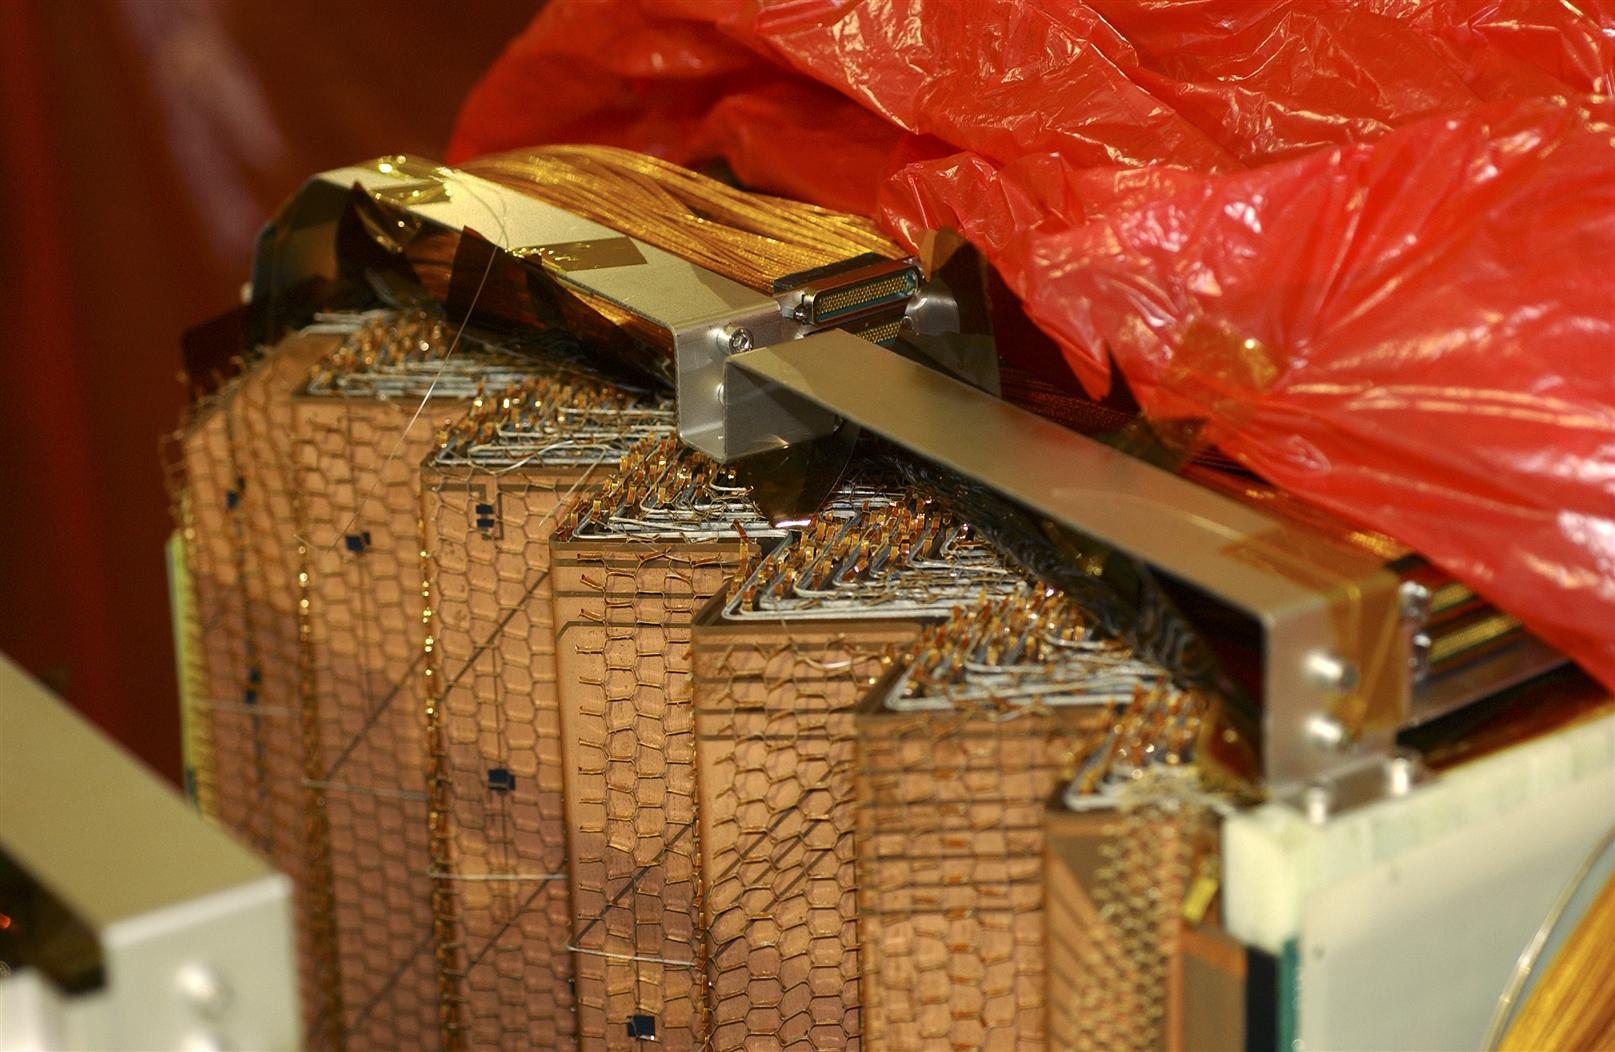
\includegraphics[width=.6\textwidth]{Detector/plots/accordion.jpg}
		\caption{A figure of the accordion-shaped electrodes.}
		\label{fig:accordion}
		\end{centering}
	\end{figure}
	%  The position of the central solenoid in
	% front of the EM calorimeter demands optimisation of the material 
	% in order to achieve the desired calorimeter performance. As a consequence, 
	% the central solenoid and the LAr calorimeter share a common vacuum vessel, 
	% thereby eliminating two vacuum walls. 
	The barrel calorimeter 	consists of two identical half-barrels, 
	separated by a small gap (4~mm) at $z$ = 0. 
	Each end-cap calorimeter is mechanically divided into two coaxial wheels: 
	an outer wheel covering the region $1.375 < |\eta|< 2.5$, and an inner wheel 
	covering the region $2.5 < |\eta|< 3.2$.
	
	The calorimeter has three layers along the transverse direction:
	a pre-sampler with very high granularity in $\eta$, in order to 
	reconstruct the neutral pions decaying to two photons and particles 
	which already starts showering in the inner detector. 
	The pre-sampler is followed by longer towers of relatively 
	high granularity, which is the major part of detecting EM showers, 
	and reponsible for measuring the $\eta$ and $\phi$ coordinates of 
	the particles. The last layer detects showers generated from 
	particles other than electrons or photons that start showering 
	inside the EM calorimeter before leaving it.

	\subsubsection{Hadronic calorimeter}
	The Hadronic calorimeter is comprised of the Tile Hadronic calorimeter (HCAL) 
	and the LAr hadronic end-cap calorimeter (HEC). 
	The HCAL is placed directly outside the EM calorimeter envelope. 
	Its	barrel covers the region $|\eta|< 1.0$, and its two extended barrels 
	the range $0.8 < |\eta|< 1.7$. It is using steel as the absorber and scintillating tiles
	as the active material. 
	% The	barrel and extended barrels are divided azimuthally into 64~modules. 
	% Radially, the tile calorimeter
	% extends from an inner radius of 2.28~m to an outer radius of 4.25~m. 
	It is segmented in depth in three layers, approximately 1.5, 4.1 and 1.8 $\lambda$ 
	thick for the barrel and 1.5, 2.6, and 3.3 $\lambda$ for the extended barrel. 
	The total detector thickness at the outer edge of the tile-instrumented
	region is 9.7 $\lambda$ at $\eta$ = 0. 
	% Two sides of the scintillating tiles are read out by wavelength shifting
	% fibres into two separate photomultiplier tubes. 
	% In $\eta$, the readout cells built by grouping fibres into
	% the photomultipliers are pseudo-projective towards the interaction region.
	
	The HEC is similar to the construction to the ECAL, using LAr as the 
	active material, but instead of using lead it uses copper as the absorber.
	It consists of two independent wheels per end-cap, located directly 
	behind the end-cap electromagnetic calorimeter and sharing the same LAr cryostats. 
	The HEC covers the range of $1.5< |\eta|< 3.2$, 
	slightly overlapping with the forward calorimeter which 
	will be described in the following paragraph 
	(around $|\eta|$= 3.1) and the tile calorimeter ($|\eta|< 1.7$).
	This overlap is to reduce the drop in material density at the transition between
	the different calorimeters.
	% Each wheel is built from 32
	% identical wedge-shaped modules, assembled with fixtures at the periphery 
	% and at the central bore.
	% Each wheel is divided into two segments in depth, for a total of four 
	% layers per end-cap. The wheels
	% closest to the interaction point are built from 25~mm parallel copper plates, 
	% while those further away
	% use 50~mm copper plates (for all wheels the first plate is half-thickness). 
	% The outer radius of the
	% copper plates is 2.03~m, while the inner radius is 0.475~m 
	% (except in the overlap region with the
	% forward calorimeter where this radius becomes 0.372~m). 
	% The copper plates are interleaved with
	% 8.5~mm LAr gaps, providing the active medium for this sampling calorimeter.
	\subsubsection{Forward calorimeter}
	The Forward Calorimeter (FCal) covers $3.1 < |\eta| < 4.9 $ and
	%  is integrated into the end-cap cryostats, 
	% as this provides clear benefits in terms of uniformity of the calorimetric 
	% coverage as well as reduced radiation background levels in the muon spectrometer. 
	% In order to reduce the amount of neutron albedo in the inner detector cavity, 
	% the front face of the FCal is recessed by about 1.2~m with respect to the EM calorimeter 
	% front face. This severely limits the depth of the calorimeter
	% and therefore calls for a high-density design. The FCal 
	is approximately 10 interaction lengths deep. 
	It consists of three modules in each end-cap: 
	the first, made of copper, is optimised for	electromagnetic measurements, 
	while the other two, made of tungsten, measure predominantly the
	energy of hadronic interactions. All three modules use LAr as active material.
	Due to high particle fluxes andenergies in the forward region, 
	the calorimeter must contain relatively long showers 
	in the small volume allowed by design constraints, 
	and thus must be very dense.
	% Each module consists of a metal matrix, 
	% with regularly spaced longitudinal channels filled with the electrode structure 
	% consisting of concentric rods and tubes	parallel to the beam axis. 
	% The LAr in the gap between the rod and the tube is the sensitive medium.
	% This geometry allows for excellent control of the gaps, which are as small 
	% as 0.25~mm in the first
	% section, in order to avoid problems due to ion buildup. 



\subsection{Muon Spectrometer}
\label{sec:MS}
The muon spectrometer is the outermost and largest sub-detector of ATLAS. 
A cut-away view of the MS is illustrated in Figure~\ref{fig:MS}.
It fully covers the	calorimeter system and occupies a large part of the ATLAS cavern. 
It is based on the magnetic deflection of muon tracks in the 
large superconducting air-core toroid magnets, instrumented with
separate trigger and high-precision tracking chambers. 
Over the range $|\eta|< 1.4$, magnetic bending is provided by the large 
barrel toroid. For $1.6 < |\eta|< 2.7$, muon tracks are bent by two smaller
end-cap magnets inserted into both ends of the barrel toroid. 
Over $1.4 < |\eta|< 1.6$, usually referred to as the transition region, 
magnetic deflection is provided by a combination of barrel and end-cap
fields. The configuration of magnets provides a field mostly orthogonal 
to the muon trajectories, hence minimising the degradation of 
resolution due to multiple scattering. 
% The anticipated high level of 
% particle flux has had a major impact on the choice and design of the spectrometer 
% instrumentation, affecting performance parameters such as rate capability, granularity, ageing
% properties, and radiation hardness.
% In the barrel region, tracks are measured in chambers arranged in three cylindrical layers
% around the beam axis; in the transition and end-cap regions, the chambers are installed in planes
% perpendicular to the beam, also in three layers.
\begin{figure}[bht]
	\begin{centering}	
	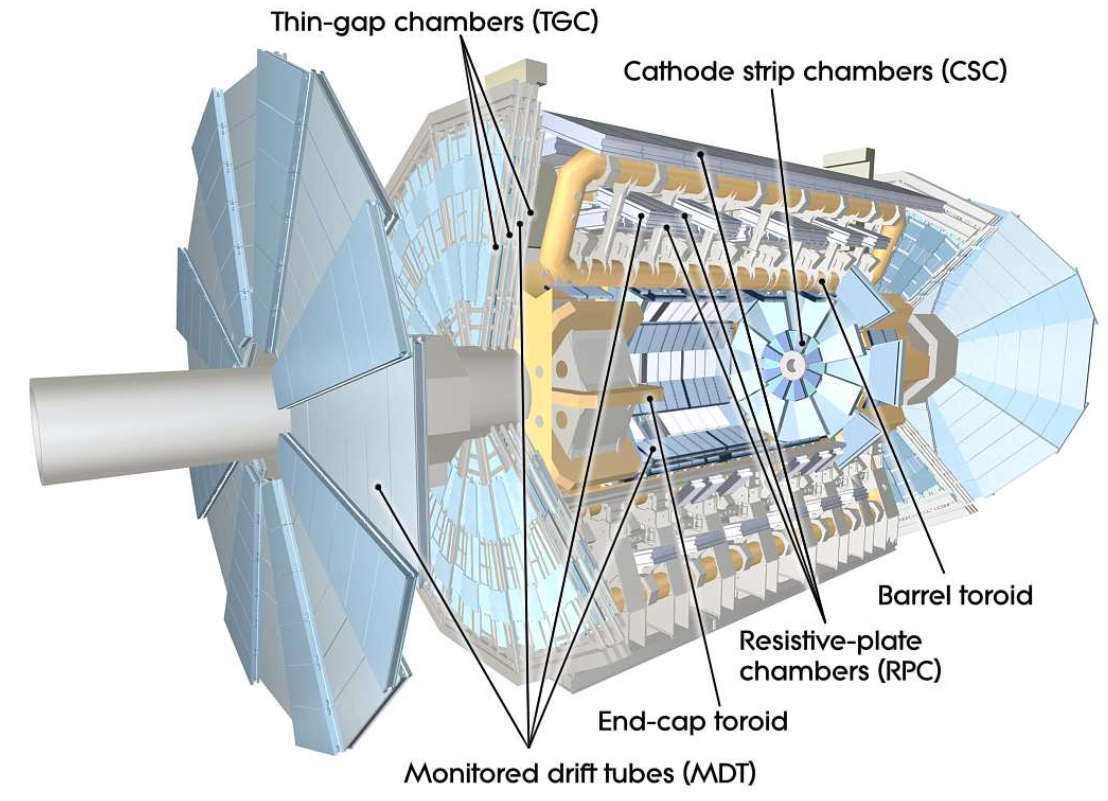
\includegraphics[width=.9\textwidth]{Detector/plots/Muon.png}
	\caption{Cut-away view of the ATLAS muon spectrometer system. Image taken from \cite{PERF-2007-01}.}
	\label{fig:MS}
	\end{centering}
\end{figure}

The MS consists of four subsystems which rely on four different gas detector
technologies. Two of them, the resistive plate chambers (RPC) in the barrel region 
and the thin gap chambers (TGC) in the end-cap region, provide trigger signals, 
while the other two, the monitored drift tubes (MDT) in the barrel and the cathode strip 
chambers (CSC) in the end-cap region provide the momentum measurement. 
The MDT chambers provide high precision measurements in the bending direction over most of the detector
acceptance while the CSC are used in the forward region where the particle flux 
is too high for the MDT	chambers. The muon chambers are arranged in the barrel 
($|\eta| < 1.05$) in three cylindrical layers around the beam axis, 
while in the end-cap regions ($1.05 < |\eta| < 2.7$) they are placed in three wheels.
The resolution of muons tracks momentum measurement varies from typically 2–3\% over
most of the kinematic range, to about 10\% at \pt\ = 1 TeV.  

\subsection{Trigger system}
% \begin{figure}[bht]
% 	\begin{centering}	
% 	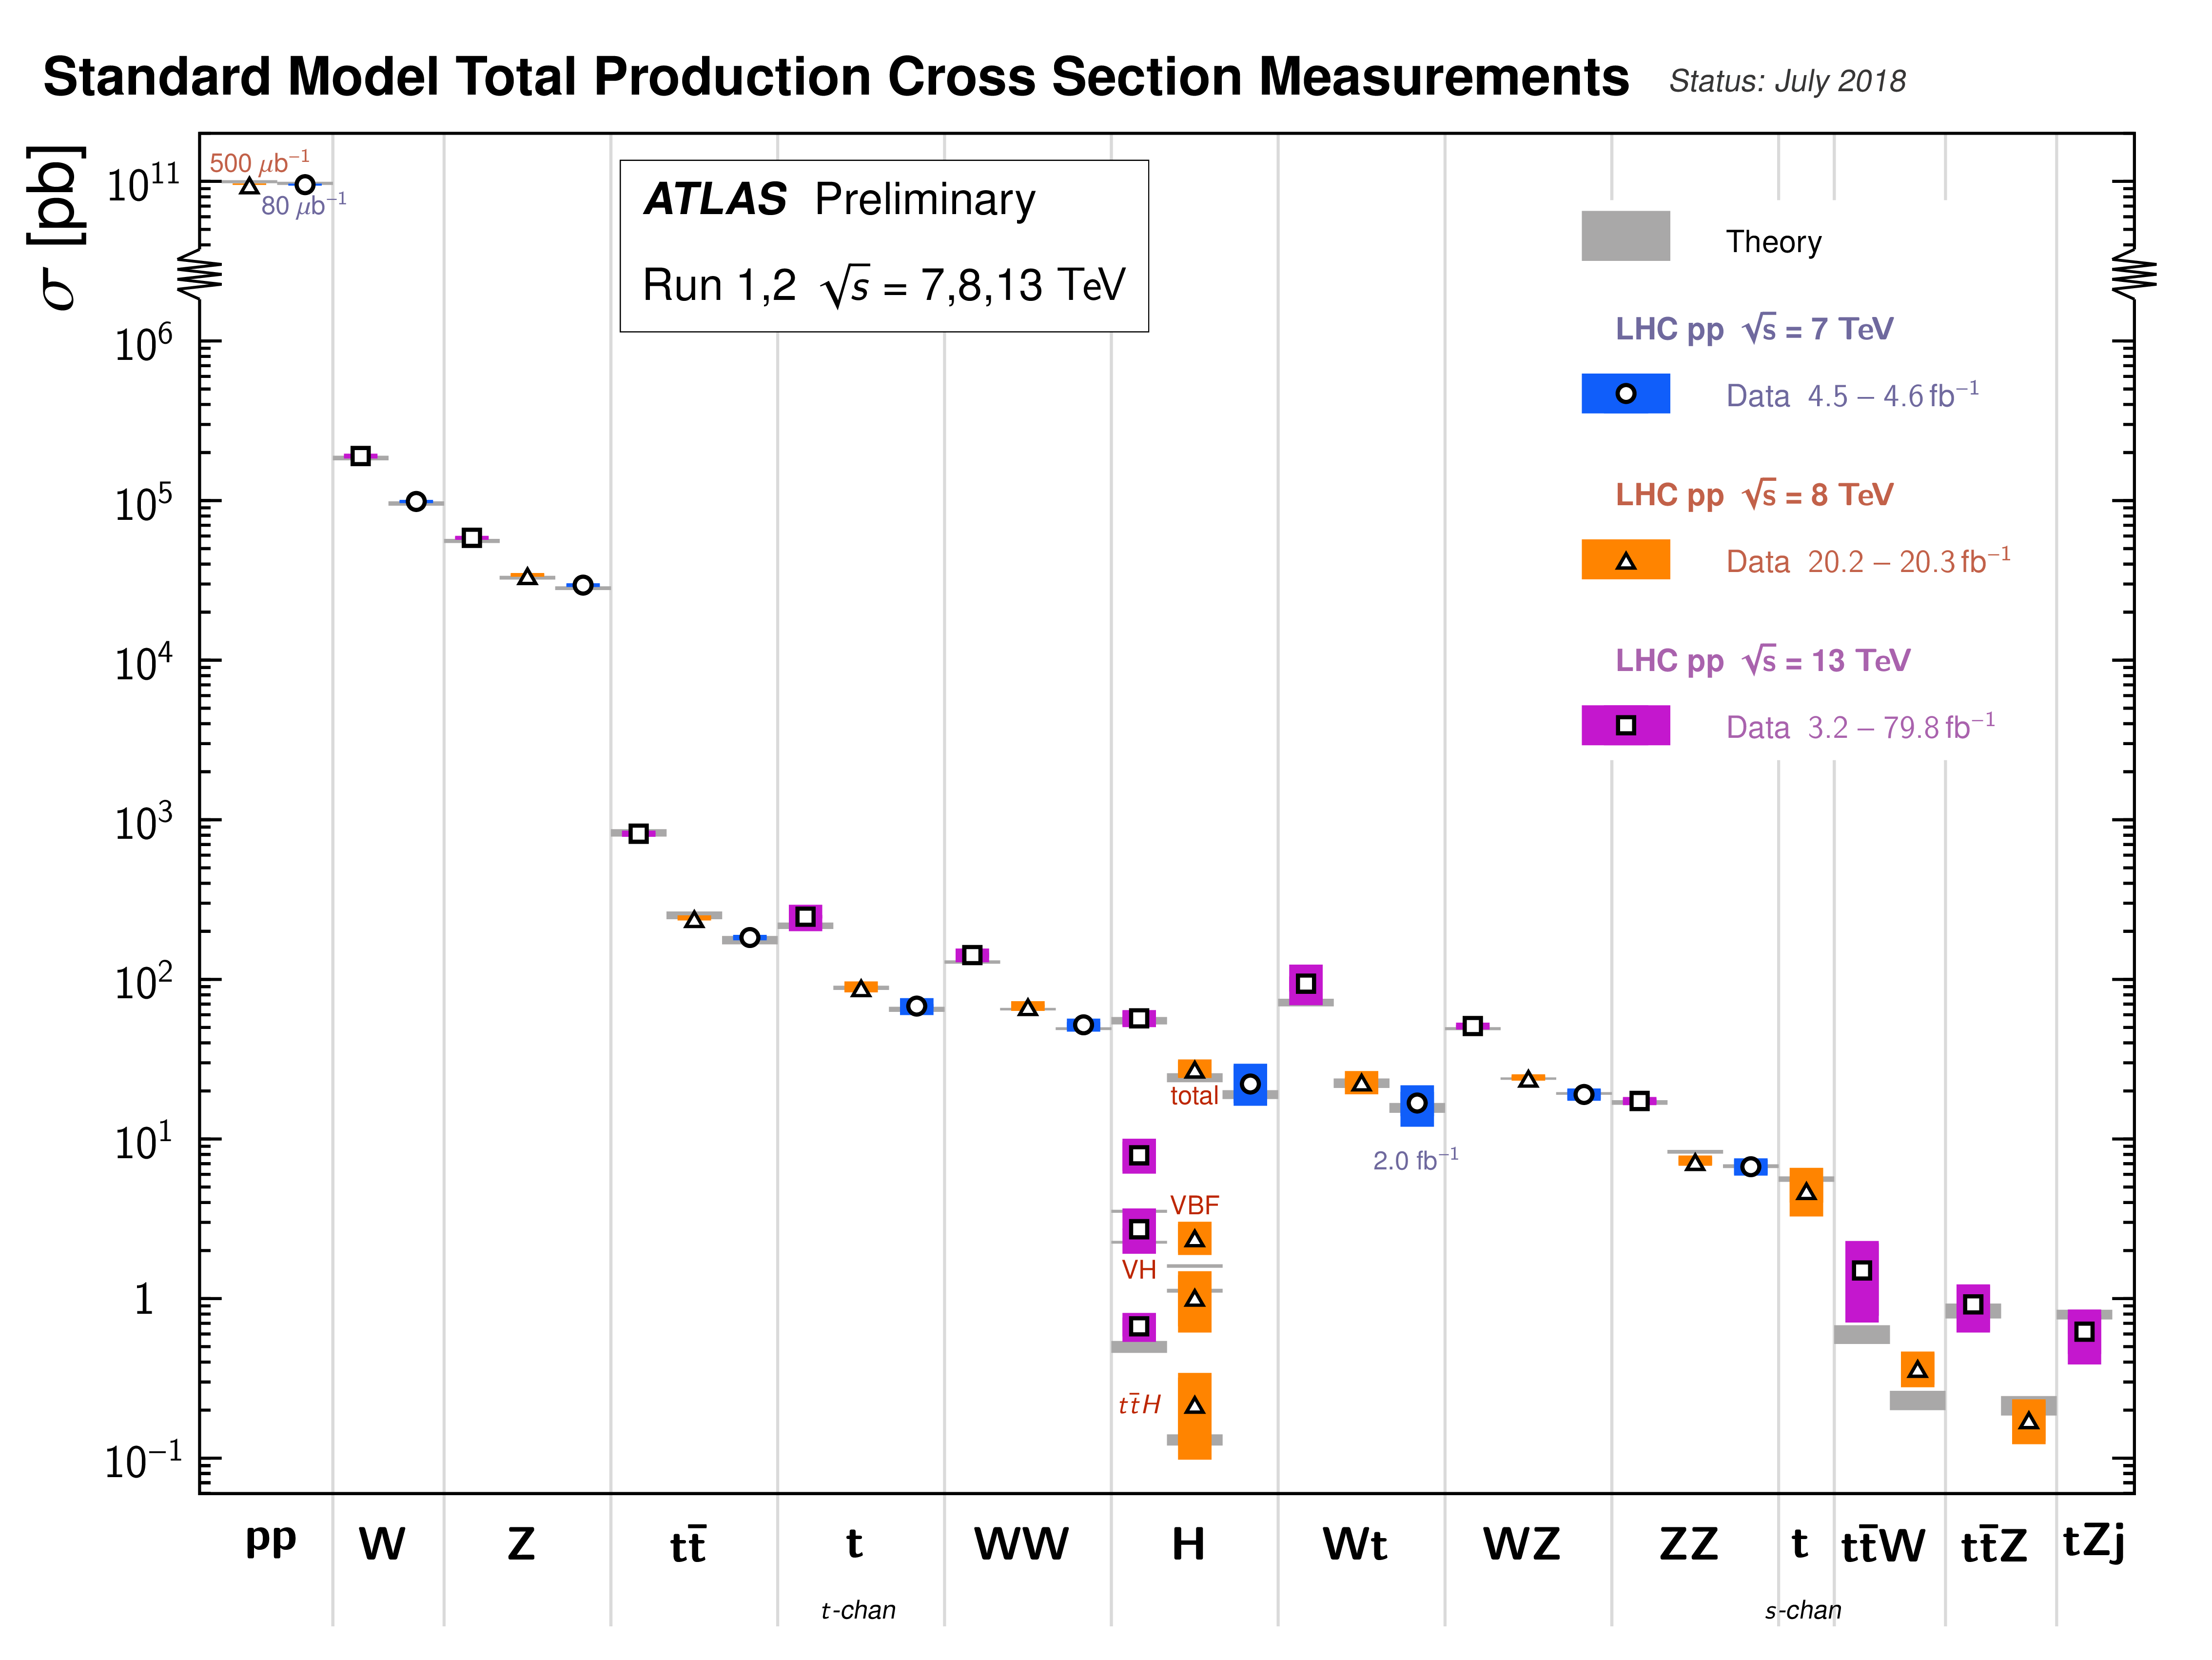
\includegraphics[width=.97\textwidth]{Detector/plots/summary xs.png}
% 	\caption{Plot showing the production cross-sections of the most dominant
% 	background processes at the LHC.}
% 	\label{fig:summary production Xs}
% 	\end{centering}
% \end{figure}
As mentioned in section \ref{sec:Operation schedule}, the spacing of each bunch
is 25 ns, which translates to a 40~MHz of bunch-crossing frequency, with up to 80
collisions per bunch crossing. This is far beyond the data collection bandwidth and 
storage capacity of ATLAS. 
% will be difficult and not meaningful to keep all these events, which includes
% a lot of ``uninteresting'' physics events. Figure~\ref{fig:summary production Xs} 
% shows a summary of the most dominant background processes production cross-sections.
% Many of these processes produce high multiplicity of jets and are not of experimental
% interest. 
Therefore, it's necessary to adopts a trigger system that make fast decisions
whether an event is high quality, rare or ``interesting'' and to save the event or not.
The ATLAS trigger system consists of two consecutive parts: the Level 1 trigger~\cite{ATLAS-TDR-12}
which is hardware-based, 
followed by the the software-based High Level Trigger (HLT)~\cite{ATLAS-TDR-16}.

The L1 trigger searches for signatures from high-\pt\ muons, electrons/photons, jets, and 
\mbox{$\tau$-leptons} decaying into hadrons. It also selects events with large MET
and large total transverse energy. The L1 trigger uses reduced-granularity information from a
subset of detectors: the RPC and TGC for high-\pt\ muons, and all the calorimeter 
sub-systems for electromagnetic clusters, jets, $\tau$-leptons, $E_{miss}^T$ ,
and large total transverse energy.
As a result, the L1 trigger reduces the event rate from 40~MHz to a maximum of 100 kHz.
The decision is made by Central Trigger	Processor (CTP), 
which operates on signals from dedicated hardware in the calorimeter
and muon detector systems. The decision time, at under 2.5 $\mu s$, is faster than the ID
can process events so ID information is omitted.
For each data-taking period, the L1	trigger is loaded with a trigger menu, 
a list of up to 256 criteria used to determine
whether an event is accepted. The trigger menus are designed to accomodate a broad
physics programme, with high acceptance for both BSM searches and SM precision
measurements.
The L1 trigger also uses detector information with reduced granularity to identify Regions
of Interest (RoI)~\cite{Blair:2007qn} in $\phi$ and $\eta$.
The ROI information with full granularity and precision and all the available detector 
data (including the ID information) within the RoI’s are provided to the HLT. 
% The HLT menus are designed to reduce the
% trigger rate to approximately 3.5 kHz, with an event processing time of about 40~ms,
% averaged over all events. 
% The final stage of the event selection is carried out by 
% the event filter, which reduces the event rate to roughly 200 Hz. 
% The selections are implemented using offline analysis procedures
% within an average event processing time of the order of four seconds.
% These events are stored and processed for later analysis. 
This trigger level reduces the rate of events by two orders of magnitude,
reaching an average of 1 kHz with a latency of 0.2 $\mu$s.
These events are passed on to a data storage system for offline analysis.


\chapter{Data and Monte Carlo samples}
\chapter{Object Reconstruction}
\large
Particles produced in the $pp$ collisions inside ATLAS can 
interact with the detector sub-systems
with each type of particle leaving a unique signature.
Reconstructing and identifying these particles precisely and efficienctly 
using the information recorded in each sub-detector is a 
building block of physics analysis.
Therefore, the following chapter outlines the reconstruction procedure of 
the particles important for the analysis present in this thesis.
\section{Track and vertex reconstruction}
\label{sec:track}
Track and vertex reconstruction is the starting point 
of physics objects reconstruction, 
which makes it crucial to understand how they are implemented in ATLAS.
Track reconstruction~\cite{ATLAS-CONF-2012-042,PERF-2015-08} is performed 
mainly with the so-called ``inside-outside'' procedure, 
complemented by the ``outside-in'' tracking and 
and the reconstruction of TRT-standalone tracks. 
% As shown in Figure~\ref{fig:electron_recon}, a charged particle traverses
% the ID. Space points are formed using the ID information.
The inside-out stage starts by assembling the raw measurements
into \textit{clusters}:
an algorithm called connected component analysis~\cite{CCA} 
groups pixels and strips in a given sensor, 
where the deposited energy yields a charge above threshold, 
with a common edge or corner into clusters. 
% It is useful to introduce the several classes of clusters identified 
% by either the ``truth information'' (TODO: remove if this is mentioned earlier in the simulation), 
% only available in simulation and referring to information at MC generator level, 
% or reconstructed quantities in both collision data and MC simulation. 
% Clusters created by charge deposits from one particle
% are called \textit{single-particle} clusters, and clusters created by charge
% deposits from multiple particles are called \textit{merged} clusters.
% These definitions rely on truth information and both cases
% are illustrated in Figure \ref{fig:cluster}. 
% In addition, clusters that are used in multiple reconstructed tracks 
% but are not sufficiently compatible with the properties of a merged cluster
% to be identified as merged by the reconstruction are called \textit{shared} clusters.
%  \begin{figure}[bth]
%     \centering
%     \begin{subfigure}[t]{.38\linewidth}
%         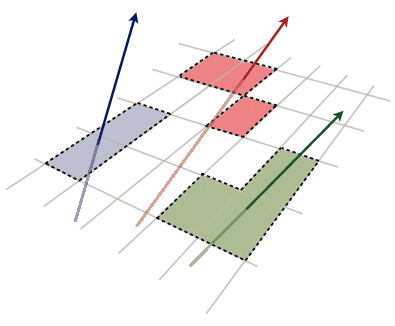
\includegraphics[width=1\textwidth]{Reconstruction/plots/single_cluster.png}
%         \caption{(a)}
%     \end{subfigure}
%     \begin{subfigure}[t]{.38\linewidth}
%         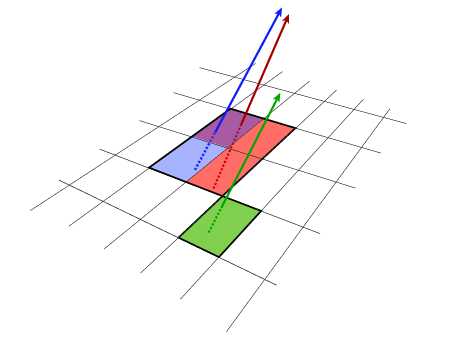
\includegraphics[width=1\textwidth]{Reconstruction/plots/merged_cluster.png}
%         \caption{(b)}
%     \end{subfigure}
    
%     \caption{Illustration of (a) single-particle pixel clusters on a pixel sensor and (b) 
%     a merged pixel cluster due to very collimated charged particles. 
%     Different colours represent energy deposits from different charged particles 
%     traversing the sensor and the particles trajectories are shown as arrows. 
%     Image taken from \cite{PERF-2015-08}.}
%     \label{fig:cluster}
% \end{figure}
From clusters, three-dimensional measurements, referred to as
\textit{space points}, are created (the yellow points in Figure~\ref{fig:track_recon}). 
They represent the point where the charged particle 
traversed the active material of the ID. 
Each space point equates to one cluster in the pixel detector, while in the SCT, 
clusters from both sides of a strip layer must be combined 
to obtain a three-dimensional measurement.
Three space points are combined to form track seeds 
(circled in blue in Figure~\ref{fig:track_recon}). 
% This approach maximizes the possible number of combinations while still allowing 
% a first crude momentum estimate. 
% The impact parameters of a track seed, 
% with respect to the centre of the interaction region, are estimated by assuming 
% a perfect helical trajectory in a uniform magnetic field.
A combinatorial Kalman filter~\cite{FRUHWIRTH1987444} is then used to 
build track candidates from the chosen seeds by incorporating additional 
space points from the remaining layers of the pixel and SCT detectors which 
are compatible with the preliminary trajectory 
(circled in a blue dashed line in Figure~\ref{fig:track_recon}). 
\begin{figure}[bht]
    \begin{centering}	
    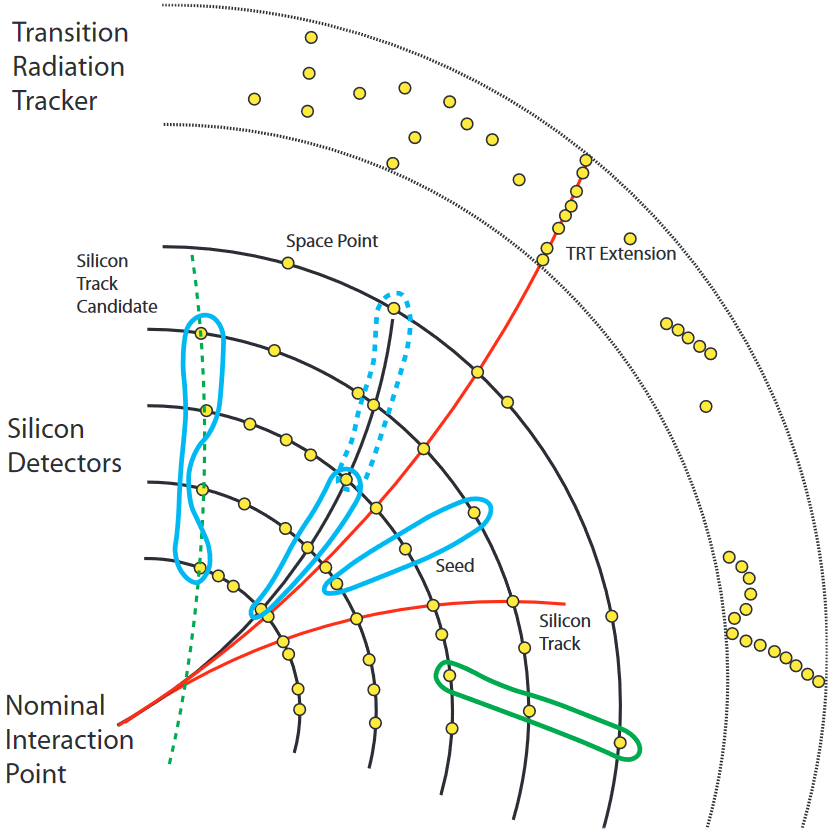
\includegraphics[width=.8\textwidth]{Reconstruction/plots/track.png}
    \caption{An example of track reconstruction. 
    Image reproduced from Ref.~\cite{ATLAS-CONF-2010-072}.
        }
    \label{fig:track_recon}
    \end{centering}
\end{figure}
A track score computed by the quantities of the fitted track
is assigned to each track.
% including the $\chi^2$ of the fitting, intrinsic resolution, 
% expected clusters multiplicity, number of holes (missing hits) 
% and \pt. 
The tracks candidates are processed in descending order of 
track score and those that fail 
a set of minimum requirements on \pt, the number of holes, 
and the number of clusters etc are rejected;
candidates that have too many bad quality clusters are 
stripped down and re-scored, then returned to the list
of remaining candidates.
This process is referred to as ``ambiguity solving''~\cite{PERF-2015-08}.
%  track candidates are fitted if they fulfil 
% a set of minimum requirement 
% on \pt\, number of holes, number of clusters etc.
% After that, the fitted tracks with too many shared clusters 
% (with additional artificial neural network to identify these shared clusters)  
% are striped down and re-scored, 
% and returned to the ordered list of remaining candidates;
% the fitted tracks with too many holes or too few clusters are rejected;
% those pass through the above requirement are accpeted and added 
% to the final track collection. 
% This process is referred to as ``ambiguity solving''~\cite{PERF-2015-08}.
Finally, the tracks are extended into the TRT and, by using the full information
of all three sub-detectors, the tracks are fitted again to determine the final track
parameters. The track can be fully represented 
by five parameters measured at the perigee,
which are the impact parameter 
(IP, transverse distance from the interaction point) $d_0$, 
the distance from the interaction point along the $z$ axis $z_0$,
the azimuthal angle $\phi$, the polar angle $\theta$ 
and the charge-momentum ratio $q/p_T$.

The complementary ``outside-in'' algorithm starts with searching for tracks with segments 
reconstructed in the TRT, and extend the tracks inwards by adding silicon hits.
The tracks are built with the combinatorial Kalman filter and passed to the
ambiguity solving procedure.
% Back-tracking is designed to reconstruct tracks of secondary particles, which are
% produced in the interactions of primary particles.
Finally, tracks with a TRT segment but no extension into the silicon detectors
are referred as TRT-standalone tracks. 

After the tracks are reconstructed, primary vertices,
which are the points where the hard-scattering processes occured,
are reconstructed in two steps~\cite{ATLAS-CONF-2010-069}:
a) the primary vertex finding algorithm, 
dedicated to associate reconstructed tracks to the vertex candidates, 
and b) the vertex fitting algorithm, 
dedicated to reconstruct the vertex position and 
its corresponding erorr matrix. 
It also refits the associated
tracks constraining them to originate 
from the reconstructed interaction point.
The vertex finding algorithm works as follows:
first, vertex seeds are obtained from the $z$-position 
at the beamline of the reconstructed tracks; 
and then, an iterative $\chi^2$ fit is then performed 
using the vertex seed and nearby tracks. 
% Each track carries a weight which is a measure of its compatibility 
% with the fitted vertex. 
Vertices are required to contain at least two tracks, and 
tracks displaced by more than 7$\sigma$ from the vertex are used to
seed a new vertex.  The procedure is repeated 
until no additional vertices can be found, 
and no unassociated tracks are left in the event.
The primary vertex for each event is selected as the vertex with the highest
$\sum_{tracks}(p_T^{track})^2$.



\large
\section{Electron}
\label{sec:electron}
When an high energy electron (or positron) enters the detector, 
it interacts with the detector material primarily via bremsstrahlung. 
This results in radiation of photons, which subsequently convert into 
electron–positron pairs which continue to 
interact with the detector material, 
leading to a cascade of particles of decreasing energy.
These cascade particles are usually referred to as electromagnetic \textit{shower}.
They are very collimated and frequently create neighbouring signals in the calorimeter component. 
% as part of the same electromagnetic cluster. 
These interactions can occur inside the inner-detector volume 
or even in the beam pipe, generating multiple tracks
in the inner detector, or can instead occur downstream 
of the inner detector, only impacting the shower in
the calorimeter. 
\subsection{Reconstruction}
% Therefore, it is possible to produce and match multiple tracks to the same electromagnetic
% cluster, all originating from the same primary electron.
The reconstruction of electron is based on three fundamental components: 
a) localised clusters of energy deposits found within the EM calorimeter, 
b) charged tracks identified in the ID (as described in details in chapter~\ref{sec:track}),
and c) close matching in $\eta \times \phi$ space of the tracks to the clusters~\cite{PERF-2017-01}.
Figure~\ref{fig:electron_recon} provides a schematic illustration of the elements that enter into
the reconstruction and identification of an electron. 
\begin{figure}[bht]
    \begin{centering}	
    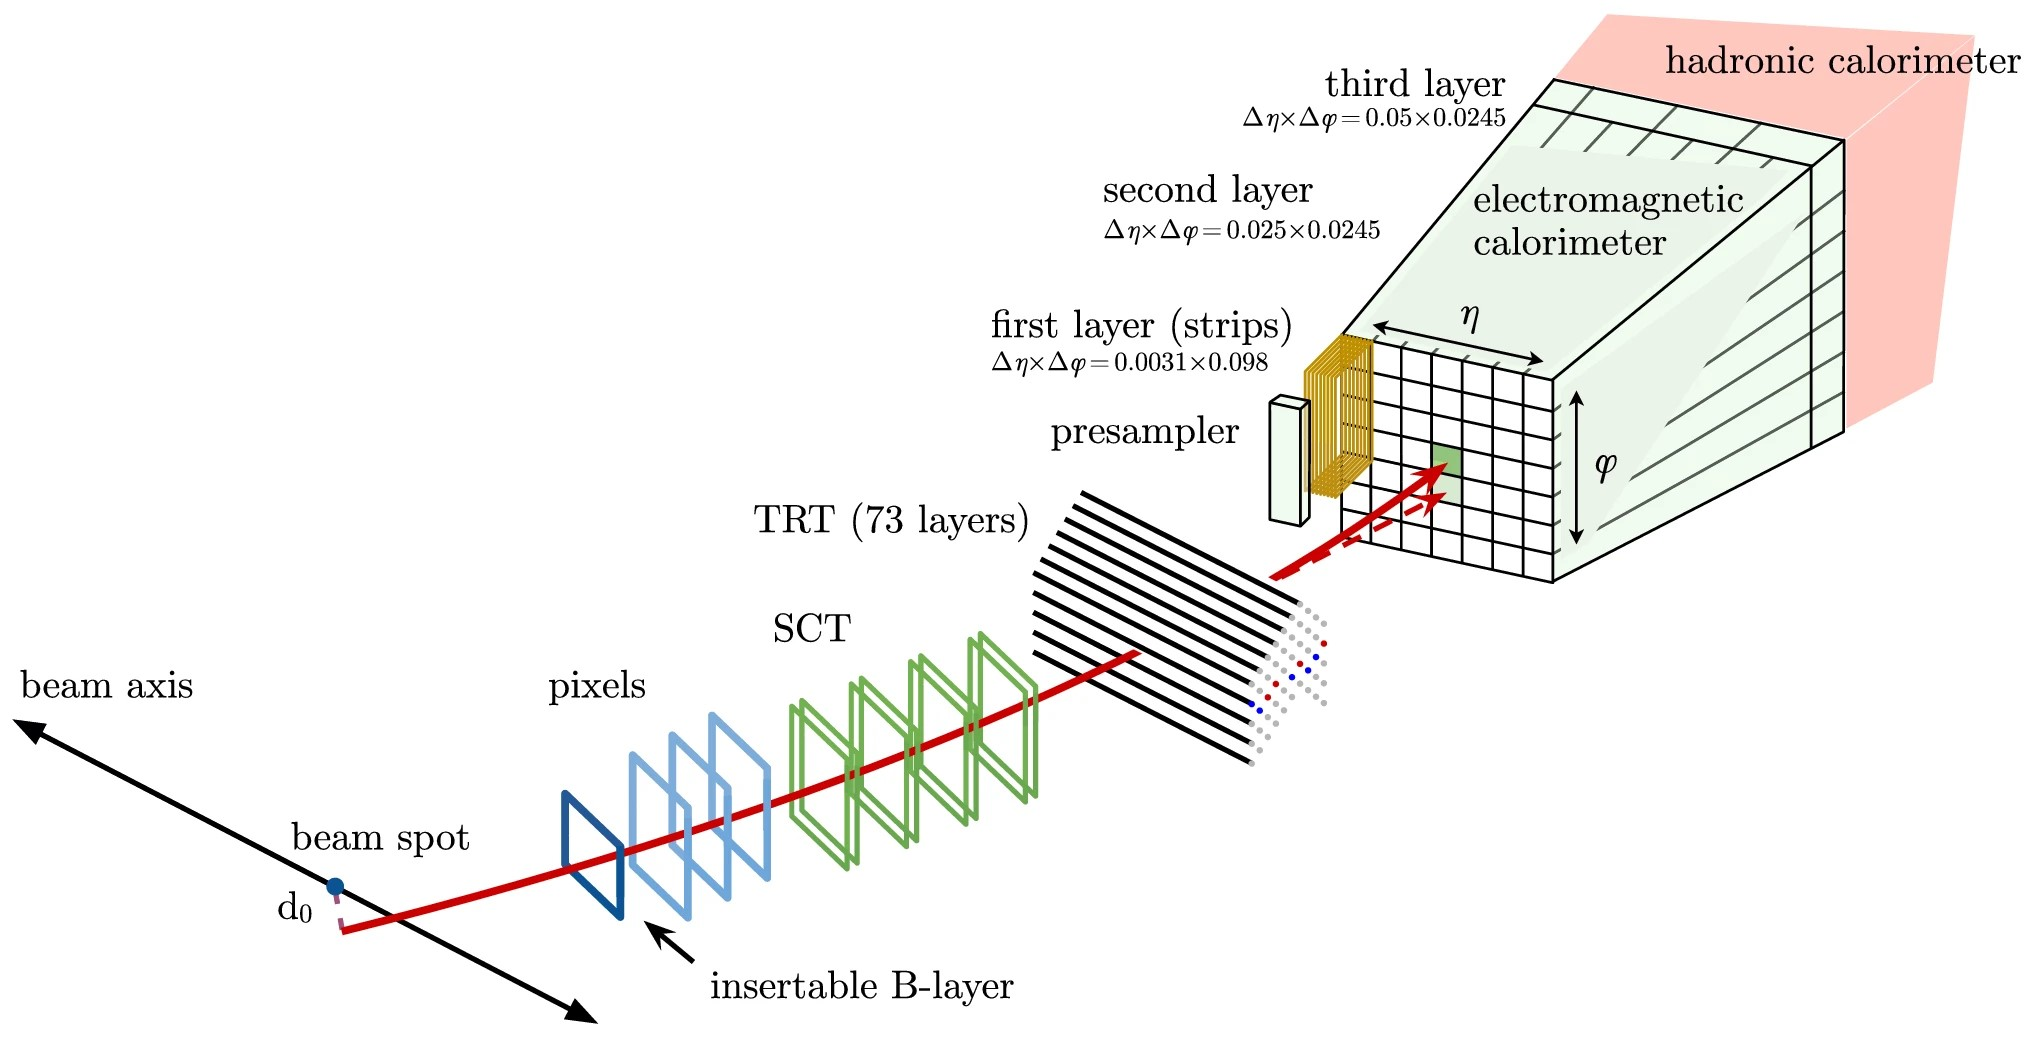
\includegraphics[width=1.0\textwidth]{Reconstruction/plots/electron.jpg}
    \caption{A schematic illustration of the path of an electron through the detector. 
    The red trajectory shows the 
    hypothetical path of an electron, which first traverses the tracking system (pixel detectors, then SCT
    and lastly the TRT) and then enters the electromagnetic calorimeter. 
    The dashed red trajectory indicates the path of a
    photon produced by the interaction of the electron with the material in the tracking system. 
    Image taken from~\cite{PERF-2017-01}.
        }
    \label{fig:electron_recon}
    \end{centering}
\end{figure}
The reconstruction starts from EM cluster seeding from localised energy deposits 
using a sliding-window algorithm~\cite{sliding-window}.
The $\eta \times \phi$ space of the EM is divided into \textit{towers} of 200 $\times$ 256
elements of size $\Delta\eta \times \Delta\phi$ = 0.025 $\times$ 0.025, 
consistent with the granularity of the second layer of the EM calorimeter. 
Then algorithm then ``slides'' a rectangular window of size 3 $\times$ 5 towers 
whose summed transverse energy exceeds 2.5 GeV to form a seed-cluster.
The centre of the seed moves in steps of 0.025 in either $\eta$ or $\phi$ direction 
to search for localised energy deposits; 
this process is repeated until every element of the calorimeter has been covered.
To better account for the energy loss of charged particles in material,
a subsequentl fitting procedure using optimised Gaussian-sum filter \cite{ATLAS-CONF-2012-047} 
is performed on tracks which are ``loosely'' matched to the EM clusters, 
which requires the tracks and clusters to satisfy:
$|\eta_{cluster} - \eta_{track}|$ < 0.05
and one of the two requirements:
$-0.20 < \Delta \phi < 0.05$ 
or
$-0.10 < \Delta \phi_{res} < 0.05$,
where $\Delta\phi \equiv -q \times (\phi_{cluster} - \phi_{track})$ with 
$q$ being the charge of the particle, and 
$\phi_{cluster}$, $\phi_{track}$ and $\eta_{cluster}$, $\eta_{track}$ 
are the $\phi$, $\eta$ coordinates of
the cluster barycentre and the poisition of the track extrapolated from the 
perigee to the second layer of the calorimeter, respectively;
$\Delta \phi_{res}$ is similar to $\Delta \phi$ but with the 
momentum of the track rescaled to the energy of the cluster.
The assymmetry in the condition is to account for the energy loss
due to bremsstrahlung where tracks with negative (positive) electric charge
bend due to the magnetic field in the positive (negative) $\phi$ direction.

The matching of the fitted tracks to the candidate calorimeter seed-cluster
is the final step of electron reconstruction. 
The matching requires $-0.10 < \Delta\phi < 0.05$,
with the other alternative requirement remaining the same.
If several tracks fulfil the matching criteria, 
the track considered to be the primary electron track is selected 
using an algorithm that takes into account the distance in $\eta$
and $\phi$ between the extrapolated tracks and the cluster barycentres 
(agian, measured in the second layer of the calorimeter), 
the number of hits in the silicon detectors and in the innermost silicon layer; 
a candidate with an associated track with at least four hits in the silicon layers and no association
with a vertex from a photon conversion (photon converting into electron-positron pair) 
is considered as an electron candidate. 
However, if the primary candidate track can be matched to a secondary vertex and has no pixel hits, 
then this object is classified as a photon candidate (likely a conversion). 

A further classification is performed using the candidate electron’s $E/p$ and \pt, 
the presence of a pixel hit, and the secondary-vertex information, to determine
unambiguously whether the object is only to be considered as an electron candidate or if it should be
ambiguously classified as potentially either a photon candidate or an electron candidate.

\subsection{Identification} 
The reconstruction algorithm is very efficient in reconstructing electron,
however, this is not necessarily what is needed for many ATLAS analysis, where
they are insterested in prompt electrons. 
Prompt electrons are electrons coming from the collision of the an event, 
while non-prompt electrons may come from
the semileptonic decays of heavy quarks or from photon conversion.
Other objects such as hadrons can be mis-reconstructed as electron as well.
It necessitates the identification of prompt electrons, making use of the 
differences between prompt electrons and non-prompt electrons/mis-reconstructed electrons.
A multivariate likelihood technique, taking advantages of the correlations
among the variables describing the differences,
is employed to select prompt electrons~\cite{PERF-2017-01}.
The input to the likelihood includes the differences of: 
a) shower shape, b) properties of the track, c) matching
of the track and clusters.
In addition, many analysis further require the electron to pass
some \textit{isolation} requirements.
Isolation is built exploiting a characteristic signature 
of the prompt electrons that 
there is relatively little activity surrounding 
the prompt electrons, as compared to non-prompt electrons~\cite{EGAM-2018-01}. 

To quantify the performance of the identification, 
the identification efficiency is measure, which represents the probability of
a prompt electron being reconstructed as an electron.
Different cuts are applied on the final discriminant
to define \textit{working points} (WP), which can specify 
the identification efficiency, as a function of $E_T$ or $\eta$ of the electron. 
Three WPs, \textit{Loose}, \textit{Medium} and \textit{Tight} are defined, 
each WP places a different requirement on final discriminant 
made with a different set of variables. 
An example of the electron identification efficiency 
is shown in Figure~\ref{fig:electron_ID}.
\begin{figure}[bht]
    \begin{centering}	
    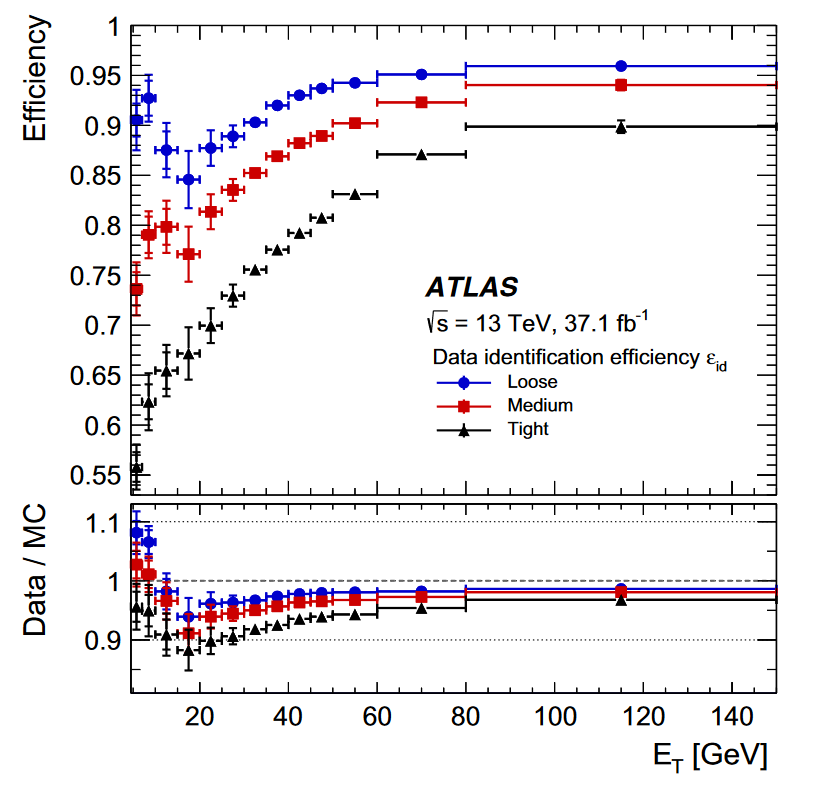
\includegraphics[width=0.45\textwidth]{Reconstruction/plots/electrond_ID1.png}
    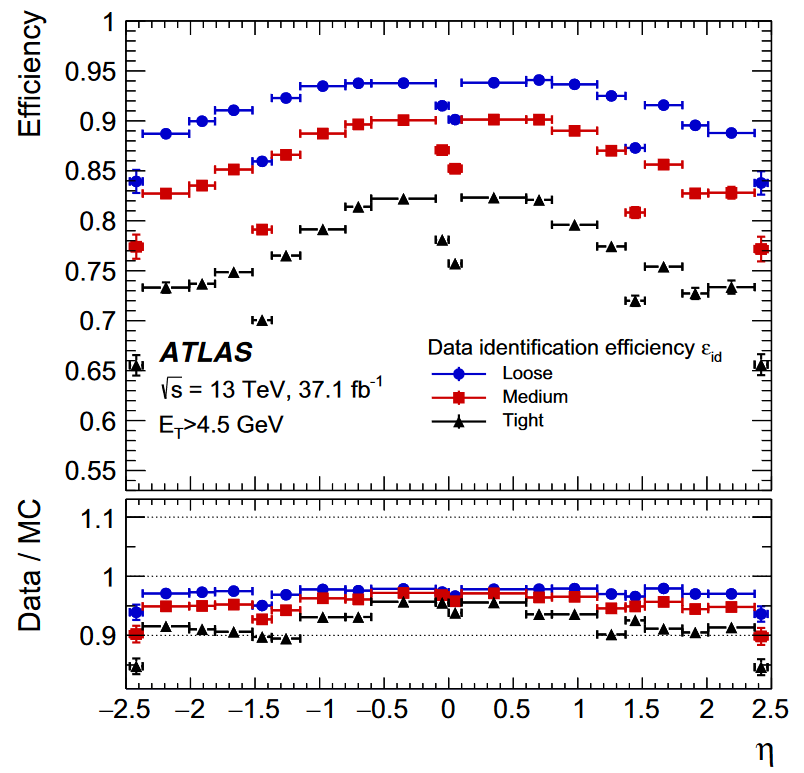
\includegraphics[width=0.45\textwidth]{Reconstruction/plots/electrond_ID2.png}
    \caption{Measured electron identification efficiencies in $Z \rightarrow ee$
    events for the `Loose' (blue circle), `Medium' (red square), 
    and `Tight' (black triangle) WPs as a function of $E_T$ (left) and $\eta$ (right). 
    The vertical uncertainty bars (barely visible because they are small) 
    represent the statistical (inner bars) and total (outer bars) uncertainties. 
    For both plots, the bottom panel shows the data-to-simulation
    ratios. Reproduced from Reference~\cite{PERF-2017-01}.}
    \label{fig:electron_ID}
    \end{centering}
\end{figure}
Similary for electron isolation, 
four WPs: \textit{Gradient}, \textit{HighPtCaloOnly}, \textit{Loose} and \textit{Tight} 
are defined, each targeting a fixed value of isolation efficiency
or imposing fixed requirement on the isolation variables. 

In the analysis presented in Chapter~\ref{sec:search for dihiggs} 
the `Loose' identification WP is used, 
with additional requirements on the electron \pt\ > 7 GeV and $|\eta|$ < 2.47;
the electron candidates are also required
to pass the ‘Loose’ isolation WP which has an efficiency of 99\%. 
The isolation requirement is also 
inverted to provide control regions for estimating backgrounds.
% , achieving 99\% efficiency 
% that is constant across the entire \pt\ spectrum.
In the calibration effort presented in Chapter~\ref{sec:FTAG} 
the `Medium' identification WP is used, 
with additional requirements on the electron \pt\ > 27 GeV and $|\eta|$ < 2.47;
electrons are required to pass the `Gradient' isolation WP,
designed to give an efficiency of 90\% at \pt\ = 25 GeV and 99\% at \pt\ = 60 GeV.
The different requirements in the two chapters 
is the result of different signal targeted and hence different 
purity and phase space is needed. 
% The `Loose' WP features variables most useful for discrimination against light-flavour jets. 
% In the `Medium' and `Tight' regimes, additional variables are added for further rejection 
% of heavy-flavour jets and photon conversions. 
% Although different variables are used for the different selections, a sample of electrons selected using a tighter LH
% is a subset of the electron samples selected using the looser LH to a very good approximation

% \textit{isolation} is built, usually by 
% summing the transverse energies of clusters in the calorimeter 
% or the transverse momenta of tracks in a cone of radius
% $\Delta R$ around the direction of the electron
% candidate, excluding the candidate itself

% The inputs to the likelihood include measurements from the tracking system, the
% calorimeter system, and quantities that combine both tracking and calorimeter information.
% The main advantages using the likelihood-based method comparing with 
% a selection-criteria-based (so-called ``cut-based'') identification is that
% a prompt electron may fail the cut-based identification because it
% does not satisfy the selection criterion for a single quantity, 
% while in the likelihood-based selection this electron can
% still satisfy the identification criteria, 
% because the likelihood combines the information of all of the discriminating variables.
% The final discriminant produced by the likelihood method is used to define 
% three \textit{working points} (WP), which are cuts in the final discriminant 
% identifying the different identification efficiencies. 






\section{Muon}
\subsection{Reconstruction}
The characteristic behaviour of a muon in the detector is a particle
ionising minimally. 
The muon reconstruction is done taking advantage of this feature, 
with information from the ID and MS tracking detectors, while
information from the calorimeters is also used
for determination of track parameters and to account for cases of
large energy loss in the calorimeters, and for MS-independent
tagging of ID tracks as muon candidates~\cite{CERN-EP-2020-199}.
The muon reconstruction consists of two steps. 
The first step is to reconstruct the stand-alone track in the MS,
followed by reconstruction with complete detector information.

The first step of reconstruction starts with the identification 
of short straight-line local track segments reconstructed 
from hits in an individual MS \textit{stations} (layers). 
These segments are then combined into preliminary track candidates, 
with information from precision measurements in the bending plane 
and measurements of the second coordinate from 
the MS triggers to create three-dimensional track candidates. 
A global $\chi^2$ fit of the muon trajectory 
through the magnetic field is performed,
outlier hits are removed and hits along the trajectory that
were not assigned to the original track candidate are added.
Finally, the tracks are fitted again with the updated hits information,
and ambiguities are resolved by removing tracks
that share a large fraction of hits with higher-quality tracks.

The second step of reconstruction is to combine the track candidates 
with the complete information of all sub-detectors.
The reconstruction proceeds according to five main
reconstruction strategies, leading to the corresponding muon
types: 
\begin{itemize}
\item \textit{combined muons} 
are identified by matching 
MS tracks to ID tracks and performing a combined track fit 
based on the ID and MS hits, taking into account the energy loss in the
calorimeters.
\item \textit{Inside out muons} 
are reconstructed using a complementary
inside-out algorithm, which extrapolates ID tracks to the MS
and searches for at least three loosely-aligned MS hits. The
ID track, the energy loss in the calorimeters and the MS hits
are then used in a combined track fit. 
% This algorithm does
% not rely on an independently reconstructed MS track, and
% therefore recovers some efficiency.
\item \textit{Muon-spectrometer extrapolated muons} are muons 
when an MS track cannot be matched to an ID track. Its parameters 
are extrapolated to the beamline and used to define an
Muon-spectrometer extrapolated muon. 
Such muons are used to extend the acceptance
outside that of the ID, thus fully exploiting the full MS 
coverage up to $|\eta|$ = 2.7.
\item \textit{segment-tagged muons} 
are identified by requiring that an ID track
extrapolated to the MS satisfies tight angular matching
requirements to at least one reconstructed MS segment. 
% A successfully-matched ID track is identified as a muon candidate, 
% and the muon parameters are taken directly from the
% ID track fit.
\item \textit{calorimeter-tagged muons} 
are identified by extrapolating ID
tracks through the calorimeters to search for energy deposits
consistent with a minimum-ionising particle.
\end{itemize}
\subsection{Identification}
Muon identification is performed by applying quality requirements that suppress background, 
mainly from pion and kaon decays, while selecting prompt muons with high efficiency.
Muon candidates originating from in-flight decays of charged hadrons in the ID 
are often characterized by the presence of a distinctive “kink” topology 
in the reconstructed track. 
As a consequence, it is expected that the fit quality of the resulting combined track 
will be poor and that the momentum measured in the ID and MS may not be compatible~\cite{PERF-2015-10}. 
Therefore, a set of requirements on the
number of hits in the different ID subdetectors and different
MS stations, on the track fit properties, 
and on variables that test the compatibility of the individual measurements 
in the two detector systems~\cite{CERN-EP-2020-199}.
A set of WPs are defined for each of the munon types defined in the 
previous section. 
The main metrics considered for designing the WPs are 
the selection efficiency and purity in simulation,
where the prompt muon efficiency of a selection WP 
represents the probability that a prompt muon traversing the detector 
is reconstructed as a muon and satisfies the WP; the purity
of a selection WP is one minus the hadron misidentification
rate (the fraction of light hadrons reconstructed as muons 
and satisfying the WP).
Three standard selection WPs: \textit{Loose},
\textit{Medium}, and \textit{Tight} are designed to 
cover the majority of physics analysis, with 
two additional WPs, \textit{High-\pt} and \textit{Low-\pt}
are designed to accommodate the analysis targeting extreme 
phase space. 
In Chapter~\ref{sec:search for dihiggs}, muons are selected
with \pt\ > 7 GeV and $|\eta|$ < 2.7, and passing the `loose' 
identification criteria as well as the `pflowLoose\_VarRadIso' 
isolation criteria~\cite{MuonWP};
while in Chapter~\ref{sec:FTAG} muons are selected
with \pt\ > 27 GeV and $|\eta|$ < 2.5, and passing the `medium' 
identification criteria as well as a track-based isolation criteria.
An example of the reconstruction and isolation efficiency of muon is 
shown in Figure~\ref{fig:muon_ID}.
\begin{figure}[bht]
    \begin{centering}	
    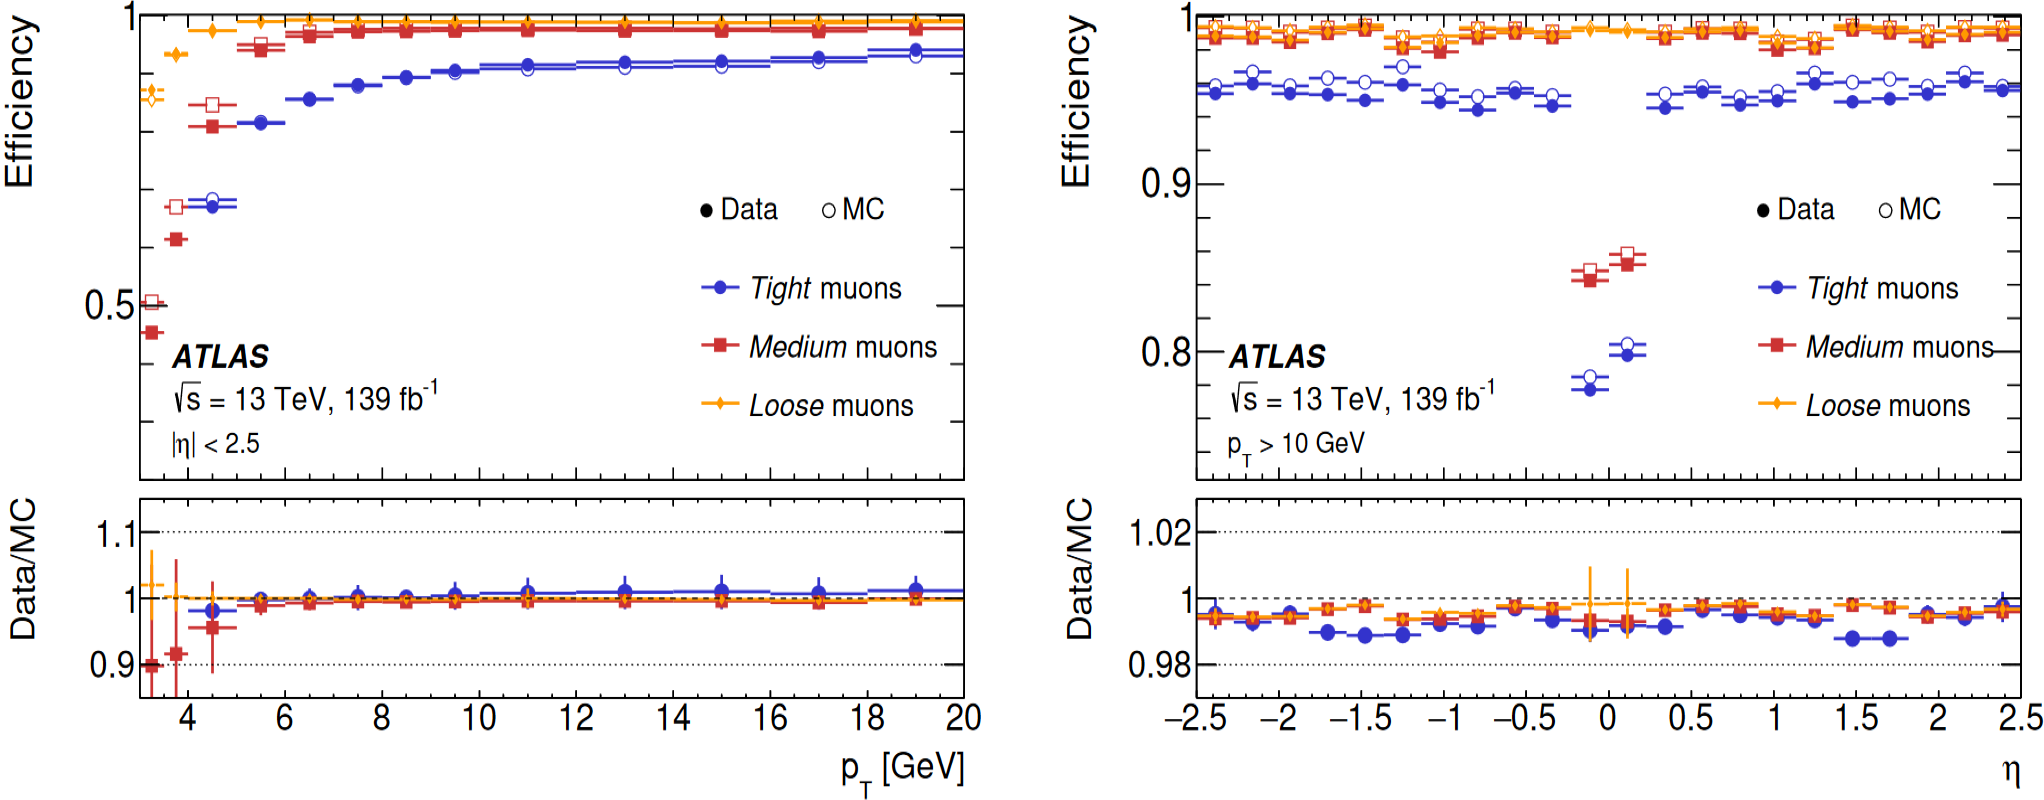
\includegraphics[width=1.0\textwidth]{Reconstruction/plots/muon_ID.png}
    \caption{
        Muon reconstruction and identification efficiencies for the Loose, Medium, and Tight criteria. 
        The left plot shows the efficiencies measured in $J/\psi \rightarrow \mu\mu$ events as function of \pt. 
        The right plot displays the efficiencies measured in $Z \rightarrow \mu\mu$ events as a function of $\eta$, 
        for muons with \pt\ > 10 GeV. The predicted efficiencies are depicted as open markers, 
        while filled markers illustrate the result of the measurement in collision data. 
        The statistical uncertainty in the efficiency measurement is smaller than the size of the markers, 
        and thus not displayed. The panel at the bottom shows the ratio of the measured to predicted efficiencies, 
        with statistical and systematic uncertainties.
    ratios. Reproduced from Reference~\cite{CERN-EP-2020-199}.}
    \label{fig:muon_ID}
    \end{centering}
\end{figure}

\section{Jets}
\label{sec:jet} 
\large
A jet can be defined as a collimated spray 
of stable particles arising from the fragmentation
and hadronisation of a parton (quark or gluon) after a collision.
Jets provide a link between the observed colourless 
stable particles and the underlying physics at the partonic
level. A basic illustration of a collision of two protons,
the subsequent particle shower and a reconstructed jet is 
shown in Figure~\ref{fig:jets}.

\begin{figure}[bht]
    \begin{centering}	
    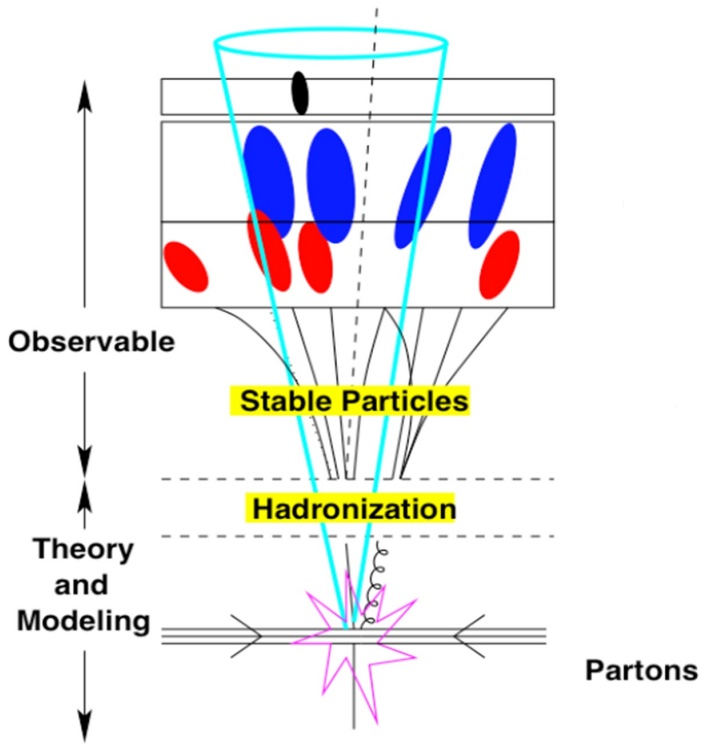
\includegraphics[width=.6\textwidth]{Reconstruction/plots/Jets.jpg}
    \caption{A simple example of an event showing the point of collision, 
    the fragmentation and hadronization of the quarks and gluons and the 
    resulting jet found through the detection of the stable particles. 
    Image reproduced from Ref.~\cite{atkin2015review}.
        }
    \label{fig:jets}
    \end{centering}
\end{figure}

\subsection{Reconstruction}
The jet reconstruction starts by forming clusters of energy deposit
in the calorimeters by performing a three-dimensional topological clustering 
of individual calorimeter cell signals~\cite{Aad_2017}.
The clustering begins with a seed cell and builds a cluster by iteratively
adding neighbouring cells, providing these cells 
have significant energy relative to the expected noise.
This algorithm clusters the energy deposits into so called ``topo-clusters'' 
and combines their four-momenta. 
In Run 1 of the LHC, the ATLAS experiment used either
solely the calorimeter or solely the tracker to reconstruct
hadronic jets and soft particle activity, 
and the vast majority of analysis utilised jets that were built 
from topo-clusters, referred to \textit{EMTopo jets}.
% These jets were then calibrated to the particle level using a jet energy scale
% (JES) correction factor [4–7]. For the final Run 1 jet calibration, this correction factor also took into account the tracks
% associated with the jet, as this was found to greatly improve
% the jet resolution [4]. 


During Run-2, an alternative approach,
called ``\textit{Particle flow}'' (PFlow) became the default
in ATLAS, as described in details in Ref.~\cite{PERF-2015-09}. 
It is also the default approach used in this thesis.
Measurements from both the tracker and the calorimeter 
are combined to form the signals. 
The particle flow algorithm provides a list of tracks 
and a list of topo-clusters.
Then, well-measured tracks are selected following a set 
of stringent quality criteria. 
The algorithm then attempts to match each track to a single topo-cluster in
the calorimeter. 
The expected energy in the calorimeter, deposited by the particle that also
created the track, 
is computed based on the topo-cluster position and the track momentum.
As a result, a new set of clusters called \textit{PFlow clusters} are produced,
matching the topo-clusters to the particles that created the high-quality tracks. 

% The energy deposited in the calorimeter by all the charged particles is removed.
% Jet reconstruction is then performed on topo-clusters
% consisting of the remaining calorimeter energy and 
% tracks which are matched to the hard interaction.
% The main advantages of integrating tracking and calorimetric information 
% into one hadronic reconstruction step is that for 
% low-energy charged particles, the momentum resolution of the tracker is significantly
% better than the energy resolution of the calorimeter (see Table \ref{tab:ATLAS_performance}).
% Above $p_T^{track}$ = 100 GeV no track information is used as the PFlow algorithm 
% becomes equivalent to EMTopo benefitting from excellent
% calorimeter performance at high energies.
% In addition, with track reconstructed, one can ascertain whether it is 
% associated with a vertex. This information can be used to mitigate 
% in-time pileup signals. 


Using the PFlow clusters as inputs, PFlow jets are then reconstructed
using the anti-$k_t$ algorithm~\cite{Cacciari_2008}. 
% The inputs to jet reconstruction are 
% the tracks that are matched to the primary vertex,
% and positive energy topo-clusters which survives the energy subtraction step 
% and matches to the selected tracks. 
The anti-$k_t$ algorithm 
sequentially combines PFlow clusters into larger clusters based on the 
momentum-weighted distance between clusters. 
For two clusters $i$ and $j$ the algorithm defines:
\[  d_{i,j} = min(p_{T,i}^{2p},p_{T,j}^{2p}) \frac{\Delta R_{i,j}^2}{R^2}   \addtag \]
and 
\[ d_{i,beam} = p_{T,i}^{2p}   \addtag \]
where $p$ is a exponent parameter and the value of -1 is used
for the anti-$k_t$ algorithm (as the name `anti' suggests),
$\Delta R^2{i,j} = (\eta_i - \eta_j)^2 + (\phi_i - \phi_j)^2 $, 
and $p_{T,i}$, $\eta_i$ and $\phi_i$ are 
the transverse momentum, 
pseudorapidity and azimuthal coordinate
of cluster $i$, respectively. 
The parameter $R$ controls the size of the jet and for standard jets 
in ATLAS this is chosen to be $R$ = 0.4.
The algorithm combines objects $i$, $j$ with minimum value of $d_{i,j}$
into one object iterartively, until no more $d_{i,j}$ can be found greater
than $d_{i,beam}$. The combined object is considered the final jet 
candidate.
% The algorithm calculates $d_{i,j}$ iterartively for all clusters: 
% when $d_{i,j} < d_{i,beam}$, the two clusters $i$, $j$ are combined
% into a single cluster, and the new cluster is added back to the list
% of consideration; when $d_{i,j} > d_{i,beam}$, the cluster $i$ is 
% considered final jet candidate and it is removed from the list of clusters.
% The anti-$k_t$ algorithm uses $p$ = -1 (as the name `anti' suggests), 
% which means that algorithm is more likely to combine two clusters with 
% very close to each other (as a result of the $\frac{\Delta R_{i,j}^2}{R^2}$ term)
% or cluster having large \pt\ with clusters having smaller \pt\ (as a result of
% the $min(p_{T,i}^{2p},p_{T,j}^{2p})$ term). 
\subsection{Calibration}
The calibration of jets starts prior to the reconstruction.
Since the energy of the calorimeter cells is measured at 
the electromagnetic scale, the local cluster weighting 
(LCW) calibration is applied to topo-clusters (before they are
used to form jets) to account for the differences in 
the detector response to hadronic and 
electromagnetic showers~\cite{CERN-PH-EP-2015-304}.

After the jets are reconstructed, the four-momenta of jets
are calibrated with the jet energy scale (JES) calibration,
which consists of several consecutive stages derived from a
combination of MC-based methods and in-situ techniques \cite{PERF-2016-04}.
MC-based calibrations correct the reconstructed jet four momentum 
to that found from the simulated stable particles 
within the jet, and in-situ techniques are used to measure 
the difference in jet response between data and simulation, 
with residual corrections applied to jets in data only.
The calibrations account for features of the
detector, the jet reconstruction algorithm, jet fragmentation,
the busy data-taking environment resulting from multiple $pp$ 
interactions, and the difference in jet response between
data and simulation.


In order to calibrate the jet energy resolution (JER),
the jet momentum must be measured precisely. 
As described in detail in Ref.~\cite{JETM-2018-05},
a \textit{dijet balance} approach is used for this purpose,
based on a well-defined dijet system,
where the two jets are expected to have \pt\ that 
sum up to zero precisely.


Furthermore, jets arising from pileup are suppressed by using the 
\textit{jet vertex tagger}, which is a multivariate 
combination of track-based variables developed to separate 
hard-scatter jets from pileup jets~\cite{ATLAS-CONF-2014-018}.


A jet cleaning selection is applied in order to veto any `fake' jets, 
which arise from non-collision background events, such as cosmic rays, 
or from detector effects. 
Finally, all jets in the analysis are required to have \pt\ > 20 GeV 
and $|\eta|$ < 2.5.


\subsection{Identification of heavy-quark flavoured jets}
\label{sec:Flavour tagging}
Known as \textit{flavour tagging}, 
the identification of jets containing $b$-hadrons (\bjets) 
against the large background of jets containing $c$-hadrons 
(\cjets) or jets coming from the hadronization of light ($u$,$d$,$s$) 
quarks or gluons (light jets) is of major importance in many areas of the 
physics programme of the ATLAS experiment at the LHC. 
It is crucial in a large number of SM
precision measurements, studies of the Higgs boson properties, and 
searches for 
new phenomena~\cite{SUSY-2014-08, ATLAS-CONF-2018-043,Interpreting_Higgs_result};
it also plays an important role in 
the $HH \to bb\tau\tau$ searches 
presented in Chapter \ref{sec:search for dihiggs}. 

% as well as the recent 
% observation of the Higgs boson decay into bottom quarks~\cite{HIGG-2018-04} 
% and of its production in association with a top-quark pair~\cite{HIGG-2018-13}. 


The ATLAS Collaboration uses various algorithms to identify 
\bjets~\cite{PERF-2012-04}, referred to as \btagging\ algorithms, 
when analysing data recorded during Run 2 of the LHC. These 
algorithms exploit the long lifetime, high mass and high decay 
multiplicity of $b$-hadrons, as well as the properties of the \bquark\  
fragmentation. Given a lifetime of the order of 1.5 ps, $b$-hadrons have a 
significant mean flight length ($\langle c\tau \rangle$ $\approx$ 450 $\mu m$), 
in the detector before decaying, generally leading to at least one vertex 
displaced from the hard-scatter collision point, as illustrated in Figure~\ref{fig:b-jet-decay}.

\begin{figure}[bth]
	\begin{centering}	
	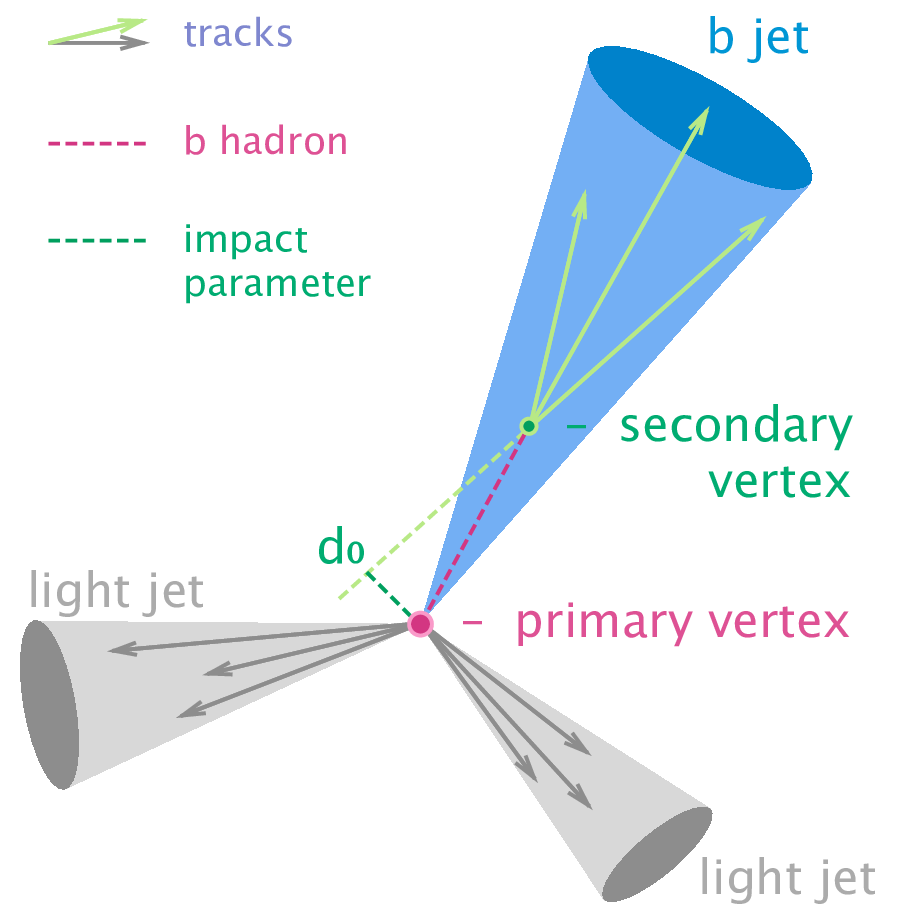
\includegraphics[width=.6\textwidth]{FTAG_plots/B-tagging_diagram.png}
	\caption{A diagram showning the b hadron decay initiated jets. }
	\label{fig:b-jet-decay}
	\end{centering}
\end{figure}


The strategy developed by the ATLAS Collaboration is based on a two-stage approach. 
Firstly, low-level algorithms reconstruct the characteristic features of 
the \bjets\ via two complementary approaches. 
A first approach, 
implemented in the IP2D and IP3D algorithms, 
is inclusive and based
on exploiting the large impact parameters of the tracks 
originating from the b-hadron decay~\cite{ATL-PHYS-PUB-2017-013}.
The second approach explicitly reconstructs displaced vertices. 
The SV1 algorithm~\cite{ATL-PHYS-PUB-2017-011}, 
attempts to reconstruct 
an inclusive secondary vertex,
while the JetFitter algorithm~\cite{ATL-PHYS-PUB-2018-025}, 
aims to reconstruct the full $b$- to $c$-hadron decay chain.
% a) using the 
% individual properties of charged-particle tracks
% associated with a hadronic jet, and 
% b) combining the tracks to explicitly reconstruct displaced vertices. 
These algorithms, first introduced during Run 1~\cite{PERF-2012-04}, 
have been improved and retuned for Run 2~\cite{FTAG-2018-01}. 
Secondly, in order to 
maximise the \btagging\ performance, the results of the low-level 
\btagging\ algorithms are combined into high-level algorithms 
via multivariate classifiers. 

The most performant algorithms presently in use in physics 
analyses at ATLAS are based on multivariate combinations 
of the available information (MV2) or additionally using a
deep feed-forward neural network (DL1)~\cite{tagging,ATL-PHYS-PUB-2017-013}.
This is illustrated in Figure~\ref{fig:b-tagging-performance}, 
where the performance
is characterised by the probability of 
tagging a \bjet\ (\bjet\ tagging efficiency, 
$\epsilon_b$) and the probability of mistakenly identifying 
a \cjet\ (light-flavour jet) as a \bjet\, 
labelled $\epsilon_c$($\epsilon_l$). 


The distribution of the output discriminant
of the MV2 and DL1 tagger for \bjets, \cjets, and light-flavour jets
in simulated \ttbar\ events are shown in Figure~\ref{fig:b-tagging-score}.
The evaluation of the performance of the algorithms is carried out using
b-jet tagging single-cut operating points (OPs, or working points, WP). 
These are based on a fixed selection requirement 
on the $b$-tagging algorithm output discriminant 
distribution ensuring a specific $b$-jet tagging efficiency, 
for the \bjets\ present in simulated \ttbar\ sample. 
The discriminant distributions are also divided into 
five `pseudo-continuous' bins, delimited by the
selections used to define the $b$-jet tagging single-cut WPs 
for 85\%, 77\%, 70\% and 60\% efficiency, and
bounded by the trivial 100\% and 0\% selections. 

Depending on the low-level algorithm, 
the DL1 tagger can be further separated into two taggers: DL1 and DL1r,
where the DL1 tagger uses traditional track-based impact parameter 
taggers IP2D and IP3D~\cite{ATL-PHYS-PUB-2016-012} 
and the DL1r tagger uses a Recurrent Neural Network Impact Parameter tagger 
(RNNIP)~\cite{ATL-PHYS-PUB-2017-013}. 


The calibration of DL1 and DL1r algorithms has been an original contribution 
of the author of this thesis and it is described in more detail in Chapter~\ref{sec:FTAG}.
The DL1r tagger is now the 
default \btagging\ algorithm used for flavour tagging in ATLAS and is
utilised in the analysis presented in this thesis.
% where performance of the algorithms is quantified 
% in terms of \bjet\ efficiency versus \cjet\ (light jet) rejections, defined as 
% 1/$\epsilon_c$ and 1/$\epsilon_l$. 


%Their high mass also leads to decay products with a larger transverse momentum relative to the jet axis with respect to the ones typically found in jets from light partons. Finally, heavy hadrons have a sizable branching ratio for semileptonic decays, hence the presence of soft leptons in the produced jets provides another tool for heavy jet identification. %The general strategy is to start with simple algorithms that exploits a particular property of b jets and progressively add more information to build moresophisticated algorithms. %The output of these algorithms consists in a discriminant value for each jet. Operating points are then defined as thresholds on the discriminant, designed to provide a determined efficiency for identifying b jets.
% Low-level $b$-taggingalgorithms fall into two broad categories. A first approach, implemented in the IP2D and IP3D algorithms~\cite{ATL-PHYS-PUB-2017-013}, or RNNIP~\cite{ATL-PHYS-PUB-2017-003} is inclusive and based on exploiting the large impact parameters of the tracks originating from the $b$-hadron decay. The second approach explicitly reconstructs displaced vertices. To maximise the $b$-tagging performance, low-level algorithm results are combined using multivariate classifiers. To this end, two high-level tagging algorithms have been developed. The first one,MV2\cite{ATL-PHYS-PUB-2017-013}, is based on a boosted decisiontree (BDT) discriminant, while the second one,DL1, is based on a deep feed-forward neural network(NN). These two algorithms are presented in fig .
\begin{figure}[bth]
	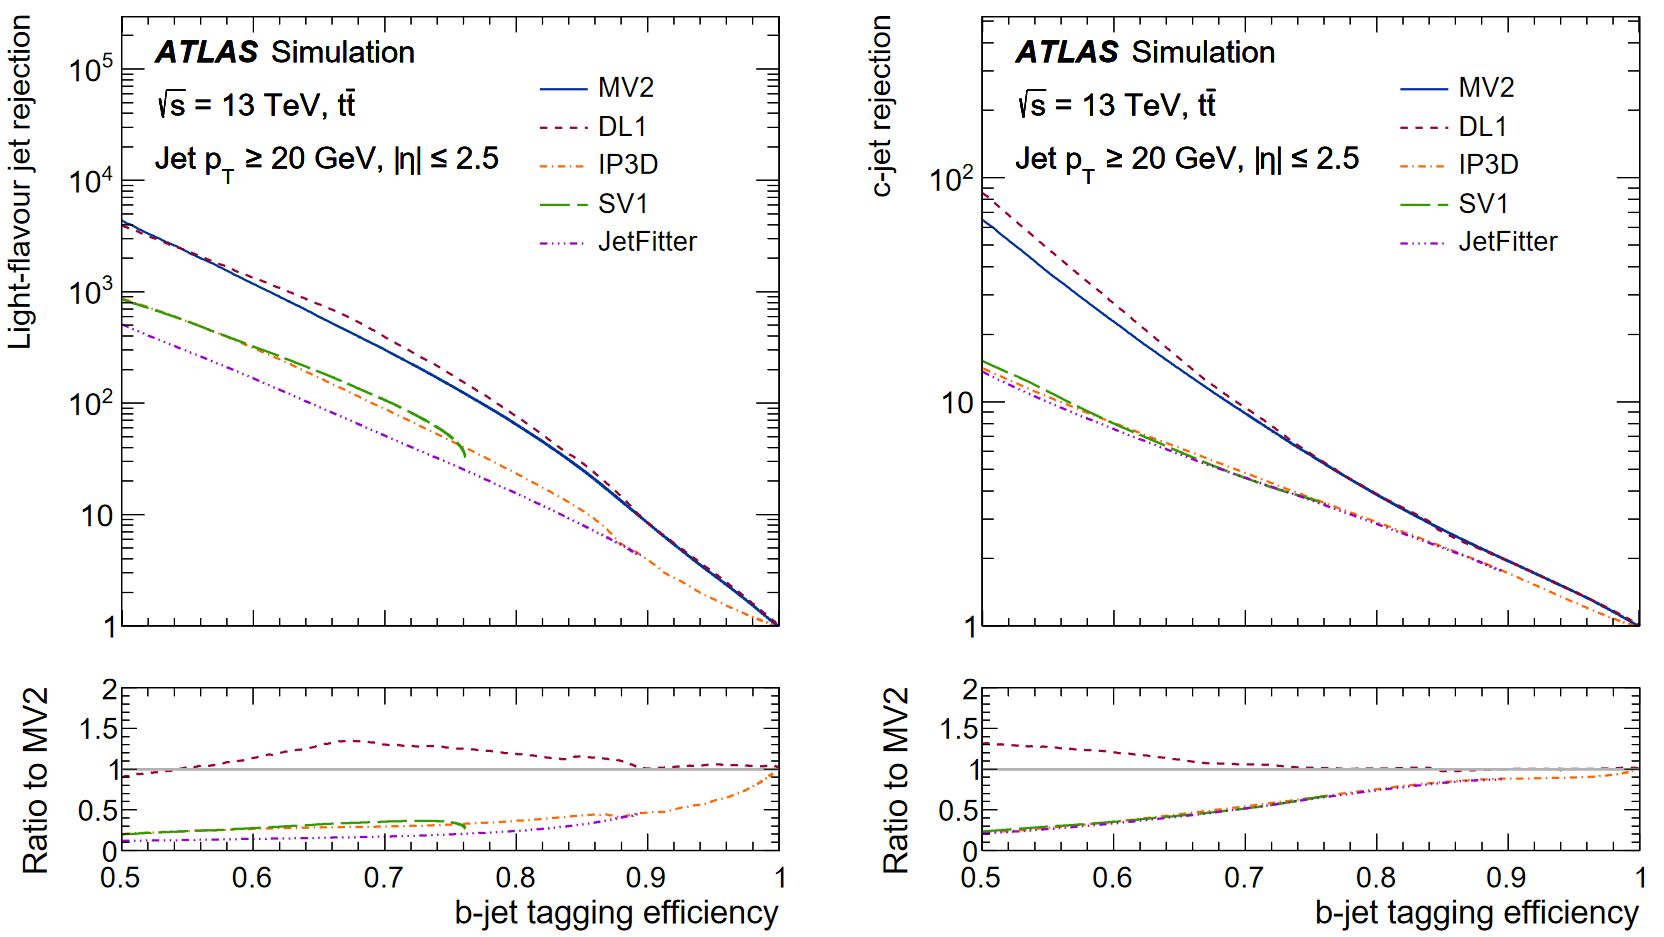
\includegraphics[width=.9\textwidth]{FTAG_plots/b-tagging-perfermance.png}
	\caption{The light-flavour jet (left) and \cjet\ (right) rejections versus 
	the \bjet\ tagging efficiency for the IP3D, SV1, \textsc{JetFitter}, MV2 and
	DL1 b-tagging algorithms evaluated on \ttbar\ events
	~\cite{FTAG-2018-01}.}\label{fig:b-tagging-performance}
\end{figure}


\begin{figure}[bth]
	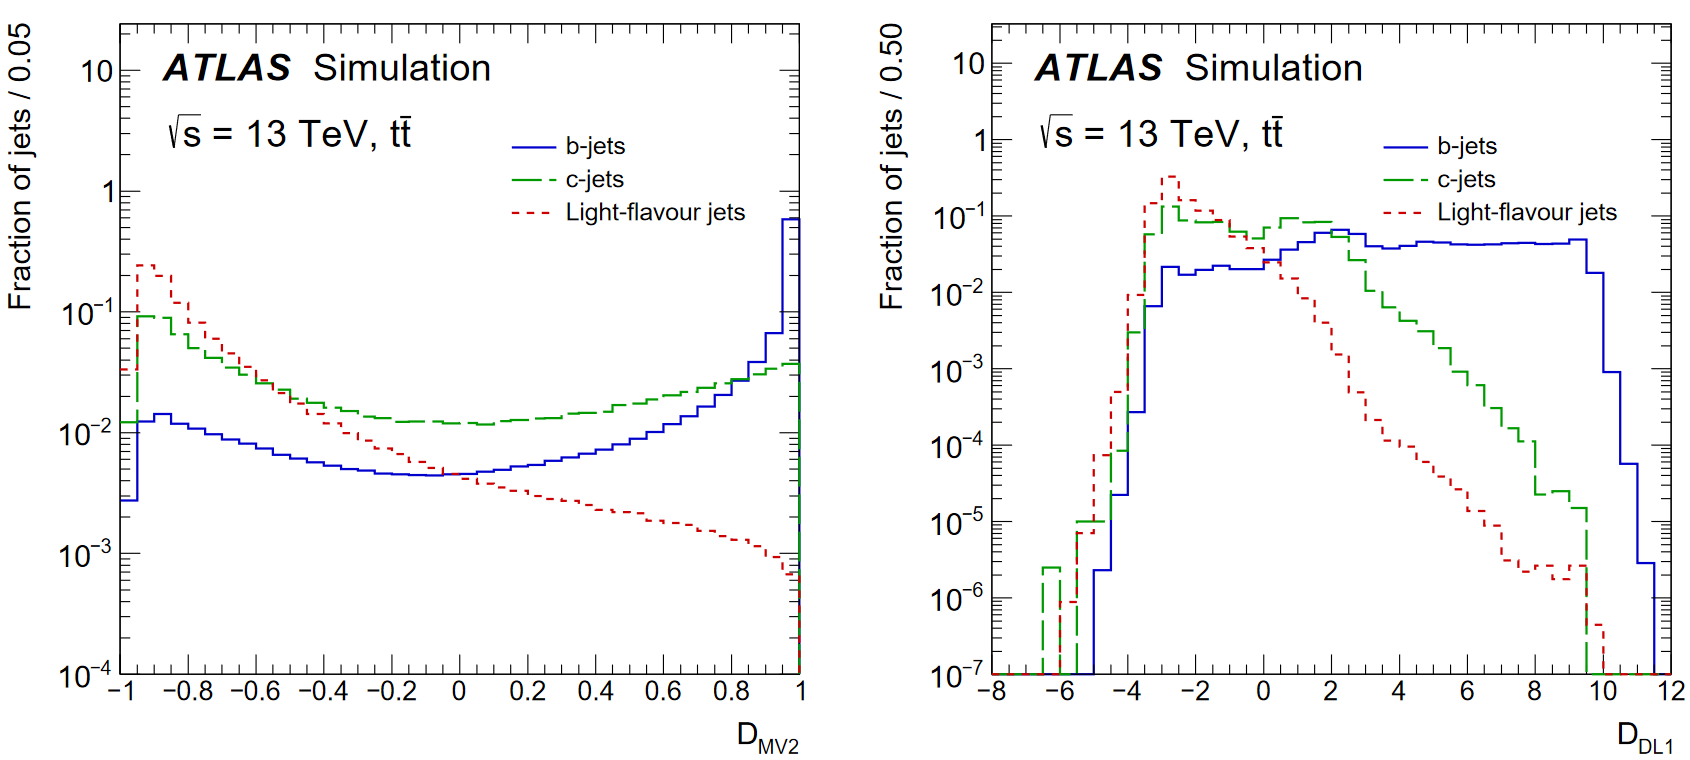
\includegraphics[width=.9\textwidth]{FTAG_plots/b-tagging-score.png}
	\caption{The fraction of light-flavour jets and \cjets\ versus 
	the \bjets\ in the MV2 (left) and
	DL1 (right) b-tagging algorithms output distribution 
	evaluated on \ttbar\ events
	~\cite{FTAG-2018-01}.}\label{fig:b-tagging-score}
\end{figure}

\large

\section{Hadronically decaying $\tau$ lepton}
\label{sec:rec:tau}
With a mass of 1.777 GeV and a proper decay length
of 87 $\mu$m~\cite{PDG}, tau leptons decay either leptonically
($\tau_{lep} \rightarrow \ell \nu \ell \nu \tau$, $\ell  = e, \mu$ ) 
or hadronically ($\tau_{had} \rightarrow$ hadrons $\nu_{\tau}$) 
and do so typically before reaching active
regions of the \hbox{ATLAS} detector. 
The leptonically decaying $\tau_{lep}$ is simply reconstructed
as either an electron or muon, with the netrinos contributing 
to the real component of the \met. 
On the other hand, the hadronically decaying $\tau_{tau}$ 
can be identified via their decay products. 
The hadronic tau lepton decays represent 65\% of all possible decay modes~\cite{PDG}. 
In these decay modes, the hadronic decay products are 
one or three charged pions in 72\% and 22\% of all cases, respectively. 
Charged kaons are present in the 
majority of the remaining hadronic decays. 
In 78\% of all hadronic decays, up to one associated neutral pion is
also produced. The neutral and charged hadrons stemming from 
the tau lepton decay make up the visible
decay products of the tau lepton, 
and are in the following referred to as $\tau_{had-vis}$.
\subsection{Reconstruction}
The $\tau_{had-vis}$ candidates are
seeded by jets formed using the anti-$k_t$ algorithm,
with a jet-size parameter $R$ of 0.4. 
For events with multiple interactions, the chosen primary may not be the
vertex where the tau lepton is originated. 
There the \textit{tau vertex association} algorithm is used with 
input as all tau candidates tracks within a region of $\Delta R$ < 0.2 
around the jet seed direction. 
The \pt\ of these tracks is summed and the 
primary vertex candidate to which the largest fraction
of the \pt\ sum is matched to is chosen as the tau vertex~\cite{ATLAS-CONF-2014-018}.

Tracks are associated with the $\tau_{had-vis}$ if they are
in the \textit{core} region $\Delta R$ < 0.2 
around the $\tau_{had-vis}$ direction and 
satisfy the following criteria: \pt\ > 1 GeV, 
at least two associated hits in the pixel layers of the inner detector, 
and at least seven hits in total in the pixel and the SCT layers. 
Furthermore, requirements are imposed on 
the distance of closest approach of the track to the track vertex
in the transverse plane, $|d_0|$ < 1.0 mm, and
longitudinally, $|z_0 sin\theta|$ < 1.5 mm. 
Tracks in the \textit{isolation} region 0.2 < $\Delta R$ < 0.4 
are used for the calculation of identification variables 
and are required to satisfy the same selection criteria.
% A set of boosted decision trees (BDTs) is used to classify all 
% tracks within $\Delta R$ = 0.4 of the $\tau_{had-vis}$ axis 
% into core and isolation tracks, depending on their \pt, 
% the number of hits in the tracking detectors 
% as well as their transverse and
% longitudinal impact parameters with respect to the tau vertex. 
The number of core tracks defines the number of \textit{prongs}.

\subsection{Identification}
The $\tau_{had-vis}$ reconstruction algorithm alone provides 
no discrimination against other particles that result in
jet-like signatures in the detector. 
Therefore, dedicated algorithms are used to identify hadronic tau lepton
decays. Here, a recurrent neural network (RNN) classifier 
is used as described in reference~\cite{ATL-PHYS-PUB-2019-033}.
Compared to the ID that was used in the analysis of the 36.1 fb$^{-1}$ data~\cite{HIGG-2016-16},
which was based on a boosted decision tree, 
the RNN tau-ID shows better performance 
and allows to move to a looser WP gaining increased efficiency 
(about 24\% and 11\% in case of two $\tau_{had}$ and 
one $\tau_{had}$ in the final state, respectively) 
without losing jet rejection, as shown in Figure~\ref{fig:RNNtau}. 
Due to the distinct signatures of 1- and 3-prong $\tau_{had}$ decays, 
the $\tau_{had}$--identification ($\tau_{had}$--ID) is split into dedicated
algorithms for 1- and 3-track $\tau_{had-vis}$.
Selected $\tau_{had-vis}$ candidates in the analysis are required to have 
\pt\ > 20 GeV, $|\eta|$ < 2.5, with candidates in the barrel-endcap 
transition region of the calorimeter (1.37 < $|\eta|$ < 1.52) vetoed 
due to poor detector instrumentation in this region, 
one or three tracks, unit charge, and to pass the ‘loose’ $\tau_{had}$--ID working point.
The loose WP corresponds to 85\% efficiency for 1-prong 
and 75\% efficiency for 3-prong (the efficiency is
flat in \pt\ by definition).
\begin{figure}[bth]
	\begin{centering}	
	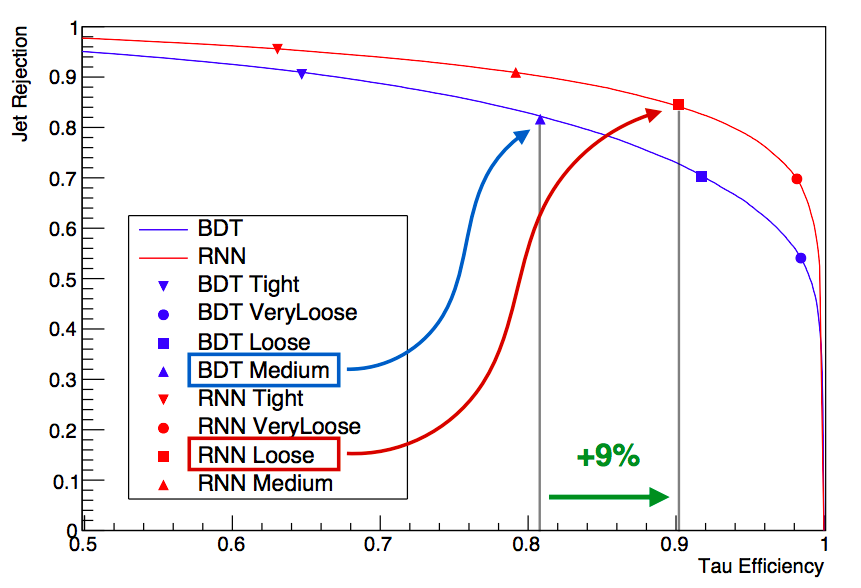
\includegraphics[width=.9\textwidth]{Reconstruction/plots/tauRNN.png}
	\caption{Jet rejection and tau efficiency of tau candidate, 
    measured in $\gamma^* \rightarrow \tau\tau$ sample for RNN-ID~\cite{ATL-PHYS-PUB-2019-033}
    and $Z/\gamma^* \rightarrow \tau\tau$ sample for BDT-ID~\cite{ATL-PHYS-PUB-2015-045}.
    Jet rejection represents the probability of a jet 
    not originating from a tau lepton being rejected 
    by the identification algorithm.
    The green arrow indicates the increase in tau efficiency.}
	\label{fig:RNNtau}
	\end{centering}
\end{figure}

Additional rejection of $\tau_{had-vis}$ candidates originating 
from electrons is provided by a BDT employing track
and shower shape information, the `loose' working point is used, 
corresponding to a selection efficiency
of about 95\% efficiency for true $\tau_{had-vis}$~\cite{ATLAS-CONF-2017-029}.
% Studies on the comparison between the BDT 
% (used in the previous round of the analysis) and RNN $\tau_{had}$--IDs
% and on the choice of the working point are reported in Appendix C.3. 

\subsection{Anti--$\tau_{had}$ definition}
In order to provide fake--$\tau_{had}$--enriched regions used for background estimation, 
an ``anti--$\tau_{had}$'' selection is defined. 
Those $\tau_{had-vis}$ objects that fail the RNN loose $\tau_{had}$--ID 
and have the RNN score greater than 0.01 are labelled as anti--$\tau_{had}$ candidates. 
For channels where $\tau_{had}$--ID is applied at trigger level, anti--$\tau_{had}$
candidates are also required to be matched to the trigger $\tau_{had}$ in 
the same way as is required for signal taus.
This definition selects objects that are 
predominantly jets faking hadronic $\tau$ decays. 
The minimum RNN score requirement ensures that 
the jets still have some $\tau_{had}$-like properties 
and ensures that the composition of quark- and gluon-initiated jets 
is closer to that of the signal region.
More details of the choice of the minimum $\tau_{had}$--ID RNN-score
threshold are reported in TODO: link to the fake factor section
% RNN score < 0.01 is chosen as it is the cut used and recommended by the Fake-Tau-Task-Force and was
% also tested here to give an improvement in the statistical precision of the multi-jet fake-factors and of the
% multi-jet template compared to the "VeryLoose" working point (RNN score < 0.05, with 95\% efficiency
% for true-$\tau_{had}$).
% Internal note C.4.1:
% The RNN > 0.01 is used by the Fake-Tau-Task-Force and has been studied here to extend the anti-tauhad
% 2526 control regions and check the impact of the reduced statistical uncertainties on the FFs and of the reduced
% 2527 statistical uncertainties on the multi-jet template.
% 2528 Lowering the cut from RNN > 0.05 of the VeryLoose to RNN > 0.01 gives an improvement in the
% 2529 statistical precision of the FFs (about 10-15% reduction in relative uncertainty) which translates in smaller
% 2530 systematic uncertainties from this source on the multi-jet template and more importantly it reduces the
% 2531 statistical uncertainty on the multi-jet tempalte itsfelf by reduced by approximately 30% given the increased
% 2532 statistics in the Anti-ID OS region where the FFs are applied to obtain the template for the SR, as shown in
% 2533 Figure 166.
\subsubsection{Anti--$\tau_{had}$ selection: TODO: should I put this section in here or in analysis chapter?}
Anti--$\tau_{had}$ objects are selected only in events 
in which there are fewer $\tau_{had}$ that pass the offline $\tau_{had}$--ID than
required for a given channel (one for the $\tau_{lep}\tau_{had}$ 
and two for the $\tau_{had}$$\tau_{had}$ selection). 
In that case, additional anti--$\tau_{had}$ candidates are selected 
so that the total number of selected $\tau_{had}$ (loose, which always has priority,
and anti--$\tau_{had}$) corresponds to the required multiplicity in each channel.
For channels where $\tau_{had}$--ID is applied at trigger level 
(more details in Section~\ref{sec:event selection}), 
only the anti--$\tau_{had}$ objects that are matched to the
trigger $\tau_{had}$ are considered, and thus there are 
no multiple selection possibilities. 
However, for channels where a $\tau_{had}$ trigger is not used, 
an anti--$\tau_{had}$ candidate is chosen randomly when there are more reconstructed
$\tau_{had}$ satisfying the anti--$\tau_{had}$ definition. 
Any anti--$\tau_{had}$ objects that are not selected in this process are also not
considered when performing the overlap removal of detector objects, 
which is discussed in Section~\ref{sec:overlap}.

\section{Missing transverse energy}
As defined in Equation~\ref{eq:MET}, the $\vec{E_T}^{miss}$ is defined 
as the negative vector sum of transverse momentum collected from the 
detector, from which one or more ``invisible'' particle(s) can be inferred. 
The reconstruction of $\vec{E_T}^{miss}$ is comprised of two contributions~\cite{MET2018}. 
The first one is from \textit{hard-event} signals combining 
information of fully reconstructed and calibrated 
physics objects, i.e. electrons, muons, photons, jets,
hadronically decaying $\tau$-leptons and jets. 
The second one is from the \textit{soft-event}, consisting of 
reconstructed charged-particle tracks associated with the hard-scatter
vertex but with no physics objects.

\section{Overlap removal}
After the event is reconstructed, an overlap-removal procedure is applied 
to resolve ambiguities when a physical object is reconstructed as multiple 
particles in the \hbox{ATLAS} detector. The angular distance $\Delta R$ is used 
to measure the overlap of two reconstructed objects.
Overlaps between most of the detector objects used in the analysis are resolved 
by using the standard overlap removal tools AssociationUtils~\cite{ORTool}, 
with analysis specific procedure for 
the reconstructed $\tau_{had-vis}$, anti-$\tau_{had-vis}$ objects and jets.
The step-by-step procedure that is used to resolve ambiguities in the 
reconstructed objects is summarised in  the following:
 \begin{itemize}
     \item  $e_1$--$e_2$: For two electrons $e_1$ and $e_2$ in an event,  
     reject $e_1$ if both electrons share the track and $p_{T1}$ < $p_{T2}$
    \item  $\tau_{had-vis}$--$e$: Reject $\tau_{had-vis}$ if $\Delta R$ < 0.2 
    % and   $e$ passes \hbox{DFCommonElectronsLHLoose}
    \item  $\tau_{had-vis}$--$\mu$: Reject $\tau_{had-vis}$ if $\Delta R$ < 0.2:
     \\ Case 1 ($\tau_{had-vis}$ $p_T$ > 50GeV): $p_T$, $\mu$ > 2GeV and combined muon
     \\ Case 2 ($\tau_{had-vis}$ $p_T$ $\leq$ 50GeV): $p_T$, $\mu$ > 2GeV
    \item  $\mu$--$e$: Reject $\mu$ if calo-muon and shared ID track
    \item  $e$--$\mu$: Reject $e$ if shared ID track
    \item  jet--$e$: Reject jet if $\Delta R$ < 0.2
    \item  $e$--jet: Reject $e$ if $\Delta R$ < 0.4
    \item  jet--$\mu$: Reject jet if $N_{track}$ < 3 ($p_{T}^{track}$ > 500MeV), and $\Delta R$ < 0.2
    \item  $\mu$--jet: Reject $\mu$ if $\Delta R$ < 0.4
 \end{itemize}
 Additionally, an analysis-specific overlap-removal procedure for $\tau_{had-vis}$, 
 anti-$\tau_{had-vis}$ and jets is implemented:
\begin{itemize}
    \item jet--$\tau_{had-vis}$: Reject jet if $\Delta R$ < 0.2
    \item anti--$\tau_{had-vis}$--jet: Reject anti--$\tau_{had}$ if jet is $b$-tagged and $\Delta R$ < 0.2
    \item jet--anti--$\tau_{had-vis}$: Reject jet if $\Delta R$ < 0.2
\end{itemize}
 This establishes the following priority: $\tau_{had-vis}$ > $b$-tagged jet > anti-$\tau_{had-vis}$ > un-tagged jet.
%  Another priority, $b$-tagged jet > $\tau_{had-vis}$ > anti-$\tau_{had-vis}$ > un-tagged jet, was investigated as an alternative
%  but found to reduce signal acceptance in the 2-tag region significantly due to limited $\tau_{had}$ rejection of the
%  DL1r $b$-tagging algorithm at the 77\% working point. With the alternative priority the signal acceptance is
%  reduced by about 8\% (13\%) in $\tau_{lep}$$\tau_{had}$ ($\tau_{had}$$\tau_{had}$).
\label{sec:overlap}

 
\chapter{Charm jet mis-tagging calibration}
\label{sec:FTAG}
\section{Calibration methods for \bjet\ and light jet}
\large
MC simulations are not able to model exactly the 
performance of the $b$-tagging algorithms in data. For this reason 
calibration is required, i.e.\ correcting MC to recover the data 
in terms of $b$-tagging efficiency, charm jet mis-tagging and 
light jet mis-tagging rates~\cite{FTAG-2018-01}. The calibration is performed 
for all supported jet collections(TODO: refer back to the object definition chapter)
and working points, which are cuts in the \btagging\ 
algorithm output identifying the different tagging efficiencies 
and corresponding light jet and \cjet rejection rate.
In general, the efficiency is calculated with data and simulations, 
and scale factors are then calculated to match the efficiency extracted 
from simulations to the data.
% The imperfect 
% description of the detector response and physics modelling effects 
% in Monte Carlo (MC) simulations necessitates the measurement of the 
% performance of the \btagging\ algorithms with collision data 
%~\cite{PERF-2012-04,ATLAS-CONF-2018-045}. 
% The measurement of the \bjet\ tagging efficiency 
% of the high-level \btagging\ algorithms used in proton–proton (pp) 
% collision data recorded during Run 2 of the LHC at $\sqrt{s}$ = 13 TeV 
% is presented. 
% The corresponding measurements for \cjets\ and light-flavour 
% jets, used in the measurement of the \bjet\ tagging efficiency to correct 
% the simulation such that the overall tagging efficiency of \cjets\ and 
% light-flavour jets match that of the data, are described elsewhere 
%~\cite{ATLAS-CONF-2018-006},~\cite{cjet}. 
The production of $t\bar{t}$ 
pairs at the LHC provides an abundant source of \bjets by virtue 
of the high cross-section and the $t \rightarrow Wb$ branching ratio 
being close to 100\%. A very pure sample of $t\bar{t}$ events can be 
selected by requiring that both $W$ bosons decay leptonically, 
referred to as di-leptonic $t\bar{t}$ decays in the following.
For the \bjet\ calibration, the performance of the $b$ tagging 
algorithms is evaluated in the simulation and the efficiency 
with which these algorithms identify jets containing $b$-hadrons 
is measured in collision data. The measurement uses a likelihood-based 
method in the di-leptonic $t\bar{t}$ sample, where
events with exactly 2 jets and 2 opposite-sign leptons are selected.  
The data \bjet\ efficiency is 
then extracted from a combined likelihood fit, and subsequently 
compared with that predicted by the simulation. Scale factors are 
then calculated to emulate the performance of the algorithms to the data~\cite{FTAG-2018-01}.

For the light jet mis-tagging calibration, two methods are 
used to measure the mis-tagging rate from the data~\cite{ATLAS-CONF-2018-006}. 
The first is the negative tag method, which uses a high statistics data sample enriched 
in light jets with the application of a modified algorithm which 
reverses some of the criteria used in the nominal identification 
algorithm.
The second is the adjusted Monte Carlo (adjusted-MC) method, which 
adjusts the characteristic track observables in the simulation 
to im the data, and then compares the adjusted simulation to the 
``standard'' simulation. The scale factors are then calculated using 
the these two methods. The scale factors of the two different methods 
are in good agreement within the systematic uncertainties. 
%The aim of this calibration is to calibrate \bjets that have been mis-tagged as light jets of \btagging\ algorithm. As the $b$-tagging algorithm is very efficient in rejecting light jets, the light jet fraction is enriched via ``flipped'' taggers, which negates the sign of track IP parameters before $b$-tagging\cite{ATLAS-CONF-2018-006}. The calibrations of the standard and the 'flipped' tagger are assumed to be equal. The calibration is extracted using the leading $p_T$ jet of Z+jets events using a 2D fit. TODO: cite the light jet tagging Int note
%light jet fractions in the $b$-like region are too low,  The Z + jets events are then selected, the secondary vertex mass is fitted to obtain flavour fractions and perform a likelihood fit to extract light jet mistag rate.
\section{Calibration method for \cjet}
\label{sec:Calibration method for charm jet}
It is worth mentioning that the author's qualification task to become an ATLAS author is to 
calibrate the rate of a charm jet being mis-identified as a \bjet\, which is a part 
of the calibration of the $b$-tagging algorithm.
During the task the calibration range has been extended down to 20~GeV (previously 25~GeV) in
jet \pt\ and a new selection category has been developed 
to increase the data statistics of the scale factors in the 
high-$p_T$ ($p_T^{jet}$ > 70~GeV) region.
The calibration is performed on the PFlow jets (as defined in Section~\label{sec:jet})
and \textit{VR-Track jets} reconstructed using the variable radius jet algorithm~\cite{VRTrackJet}.

As determined by the CKM matrix~\cite{CKM1,CKM2}, the $W$ boson decays dominantly to 
a pair of light quarks ($u$ quark and $d$ quark) or to
a $s$ quark and a \cquark. The $W$ boson decays very rarely to pairs containing a \bquark. 
More specifically, the branching ratio of a $W$ boson decays to a $u$ quark and $d$ quark pair or 
a $s$ quark and $c$ quark pair is 33.1\%, and to pairs containing a $b$ quark is only 0.057\%~\cite{PDG}. 
Therefore, $b$-tagged jets from the $W$ decay are most likely 
to be mis-tagged \cjets or light jets. 

Furthermore, given the ratio between the DL1 light jet rejection and the corresponding charm jet rejection 
ranges from 10 to 40 (Figure~\ref{fig:b-tagging-performance}), the 
\cjet\ is much more likely to be mis-tagged than the light jet. 
This allows for a source of mis-tagged \cjets to be obtained in the \ttbar\ events, 
requiring that one $W$ boson decays leptonically and the other decay hadronically 
(referred to as semi-leptonic $t\bar{t}$ decay in the following),
where the $b$-tagged jets from the $W$ decay are candidates of mis-tagged \cjets.
Requiring a $W$ boson decaying leptonically 
reduces the number of combinations of jets of different flavour, 
and allows triggering with the lepton.

The events kinematics are shown by the diagram in 
Figure~\ref{fig:feynman}, where the \ttbar\ pair decays to a 
$b$ and a $\bar{b}$ quark, circled in red. One of the $W$ bosons, 
circled in blue, decays hadronically to quarks, 
and the other $W$ boson decays leptonically to either 
an electron or a muon and the corresponding neutrinos, 
circled in green and purple, respectively. 
The lepton in the final state is used for triggering.
The following notation will be used: the jets that are
the decay products of the $W$ boson are referred to as
$W$ jets and the remaining two jets are referred to as top-jets.

\begin{figure}[H]
\centering
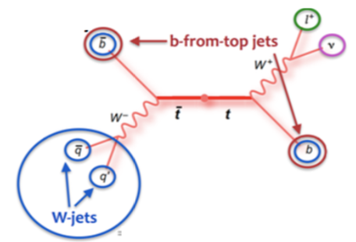
\includegraphics[width=.45\textwidth]{FTAG_plots/feynman.png}
\caption{Feynman diagram of the semi-leptonic $t\bar{t}$ events.}
\label{fig:feynman}
\end{figure}

%As Shown in Fig \ref{fig:feynman}, the calibration uses the semi-leptonic $t\bar{t}$ events, which one $W$ boson from top decays leptonically to a charged lepton and neutrino and one $W$ decays hadronically and dominantly to a charm and a strange quark, among other pairs.

A kinematic likelihood technique, referred to as 
KLFitter~\cite{ERDMANN201418}, is used to assign jets to the proper $t\bar{t}$ decay product 
(more details in Section \ref{KLFitter}). 
The following notation will be used: the jets that are
assigned as the decay products of the $W$ boson are referred to as
$W$ jets and the remaining two jets are referred to as top jets.


The charm jet efficiency is defined as the ratio of events with either of the 
\wjet\ is tagged. The efficiency is evaluated in four \pt\ intervals, with 
boundaries of 20, 40, 65, 140 and 250~GeV for the PFlow jets and 15, 20, 40, 140~GeV
for the VR-Track jets; and for four tagging intervals with the boundaries of 85\%, 77\%,
70\% and 60\%. 

The choice of the bin boundaries ensures enough statistics for each bin and 
hence relatively flat statistical uncertainty, 
given the underlying charm-jet \pt\ spectrum as shown in Figure~\ref{fig:kinematic_distributions_combined}.
The boundaries for the VR-Track jets are lower than for PFlow jets, 
since the track jets miss the neutral particles the
reconstructed energy is significantly below the true jet energy.

The main method described in the chapter is for the ``fixed-cut'' calibration
where the efficiency is defined as the fraction of \bjets passing the tagger.
Jets are said to be tagged (untagged) at particular working point
if they have DL1r scores greater (less) than the DL1r score of that working point.
The events with both \wjet\ are discarded to simplfiy the fit described in the following.

To extract the scale factors of the charm jet mis-tagging, a fit is performed by minimising 
the $\chi^2$ defined as:
\begin{eqnarray*}
\chi^2 = \sum_{t=1}^4 \sum_{i=1}^4  \sum_{j=1}^4 (N^{t}_{\mathrm{data}}(i,j)- p(i,j) [c^{t}(i)N^{t}_{C}(i,j)+N^{t}_{J}(i,j)
\end{eqnarray*}
\begin{eqnarray*}
	+ \sum_k  c^{4}(k) N^{t}_{X}(i,j,k)])^2/N^{t}_{\mathrm{data}}(i,j)
\end{eqnarray*}
\begin{eqnarray}
 +  \sum_{i=1}^4 \sum_{j=i}^4 [N^{\mathrm{untag}}_{\mathrm{data}}(i,j)-p(i,j)N^{\mathrm{untag}}_{\mathrm{MC}}(i,j)]^2/N^{\mathrm{untag}}_{\mathrm{data}}(i,j).
\label{eqn:chi2}
\end{eqnarray}
The $c^{t}(i)$ is the main floating parameter in the fit, which is the charm jet 
mis-tagging scale factor at working point $t$ of \pt\ bin labelled $i$. 
The other main floating parameter is $p(i,j)$ that is the normalisation factor scaling the MC to
data. 
The $N^{t}_{\mathrm{data}}(i,j)$ is the number of data events with a tagged \wjet\ in the \pt\ bin labelled i
and the other (untagged) \wjet\ in the \pt\ bin labelled j. Similarly the $N^{t}_{C}(i,j)$ is the number of MC events 
with a tagged \wjet\, while the tagged \wjet\ is indeed a \cjet\, which can be seen as ``signal''. 
In contrast the $N^{t}_{J}(i,j)$ is the number of events with neither the tagged \wjet\ nor the top jets 
are \cjets\; and the $N^{t}_{X}(i,j,k)$ is the number of events with one of the top jets is a \cjet\. 
These two types of events can be seen as ``background''. The later case is slightly more complicated, as the 
\cjet\ lies in a different \pt\ bin to the tagged jet, denoted as $k$, and it only depends on the 
$c^4(k)$ (which is the scale factor of the 4th working point i.e. 60\% ) as the top jets
are tagged at 60\% working point. 
The calibration is then given as the scale factors of the four working points 
in bins of \pt\ defined in the above text. 

% The charm-jet efficiency of the MC can be extracted from the truth information which indicates the 
% true nature of the $W$ jets. The \cjet\ efficiency of the MC is defined as the probability a true \cjet\ 
% is tagged by the \btagging\ algorithm in bins of jet \pt. 
% The charm-jet efficiency of the data is extracted by applying a combinatorial likelihood fit to $W$ jets, 
% where the main floating parameter are the \cjet\ efficiency
% in a given \pt\ bin and the ratio of data over total MC. 
% The calibration is given as scale factors in bins of \pt\ for 4 fixed-cut working points (WP) 
% that scale the simulation shape to reproduce that of the data, where the
% scale factors are calculated as the ratio of the data charm-jet efficiency over 
% the MC charm-jet efficiency. The calibration is performed for 4 \pt\ bins  
% (20, 40, 65, 140, 250) for the PFLow jets and (10, 20, 40, 65, 140) for the VR-Track jets
% in units of GeV. 

\section{Data and Monte Carlo samples}
%%%%%%%%%%%%%%%%%%%%%%%%%%%%%%%%%%%%%%%%%%%%%%%
\label{sec:samples}
TODO: remove the overlap between this section and the Data MC chapter in the thesis
Dedicated MC are used to model SM processes. 
%%%%%%%%%%%%%%%%%%%%%%%%%%%%%%%%%%%%%%%%%%%%%%%
The data analysed in this study correspond to 139~fb$^{-1}$~\cite{DAPR-2010-01,DAPR-2011-01,DAPR-2013-01,LUCID2}, 
of \(pp\) collision data collected by the ATLAS detector between 2015 and 2018
with a centre-of-mass energy of 13~\TeV. 
The data sample was collected using a set of single-muon~\cite{Aad:2020uyd} 
and single-electron triggers~\cite{TRIG-2018-05}. The single-muon triggers 
had \pt\ thresholds in the range 20--26~\GeV\ for 
isolated muons and 50~\GeV\ for muons without any isolation requirement. 
The single-electron triggers employed a range of \pt\ thresholds 
varying between 24--300~\GeV\ 
and a combination of quality and isolation requirements depending on the 
data-taking period and the \pt\ threshold.
%The uncertainty in the combined 2015--2018
%integrated luminosity is 1.7\%~\cite{ATLAS-CONF-2019-021}, obtained
%using the LUCID-2 detector~\cite{LUCID2} for the primary luminosity
%measurements. 
All detector subsystems were required to be operational
during data taking and to fulfil data quality requirements.  

% The $t\bar{t}$ samples and the single top-quark in the Wt 
% and s-channel samples are generated with the {\tt Powheg-Box} v2~\cite{powheg} 
% generator. Electroweak t-channel single top-quark events are generated 
% using the {\tt Powheg-Box} v1~generator. The parton shower, fragmentation, 
% and the underlying event are simulated using {\tt Pythia} 6.428\cite{pythia} 
% with the CTEQ6L1 PDF sets and the corresponding Perugia 2012 tune (P2012)~\cite{perugia}. 
% The top-quark mass is set to 172.5~GeV. The {\tt EvtGen} v1.2.0 program~\cite{evtgen} 
% is used to model the properties of the bottom and charm hadron decays. 
% The $t\bar{t}$ production cross-section is calculated at NNLO+NNLL 
% (next-to-next-to-leading-logarithm)~\cite{NNLO}. For single-top processes, 
% the generator NLO cross-sections are used. Events containing $W$ or $Z$ 
% bosons with associated jets are simulated using {\tt Sherpa} 2.2.1\cite{sherpa}. 
% All $W$/$Z$+jets events are normalised to the predicted cross-sections using 
% NNLO calculations. All samples are passed through the full GEANT4\cite{GEANT4} 
% simulation of the ATLAS detector and are reconstructed with the same software as used for data.



All samples were 
produced using the ATLAS simulation infrastructure~\cite{SOFT-2010-01}
and $\GEANT4$~\cite{Agostinelli:2002hh}. A subset of samples use a faster 
simulation based on a parameterisation of the calorimeter response and 
$\GEANT4$ for the other detector systems~\cite{SOFT-2010-01}. %\cite{ATL-PHYS-PUB-2010-013}.
The simulated events are reconstructed with the same algorithms as
used for data, and contain a realistic modelling of pile-up
interactions. The pile-up profiles in the simulation match those of each dataset
between 2015 and 2018, and are obtained by overlaying minimum-bias events,
simulated using the soft QCD processes of
{\PYTHIA}~8~\cite{Sjostrand:2014zea} using the NNPDF2.3LO set of
PDFs~\cite{Ball:2012cx} and a set of tuned
parameters called the A3 tune~\cite{ATL-PHYS-PUB-2016-017}.

The events that are used in this study originate mostly due to 
\ttbar\ production. This process is modelled using the
\powhegbox~v2~\cite{Frixione:2007nw,Nason:2004rx,Frixione:2007vw,Alioli:2010xd}
generator at NLO with the \nnpdfnlo % ~\cite{Ball:2014uwa}
parton distribution function (PDF) set
and the \hdamp\ parameter\footnote{The
  \hdamp\ parameter is a resummation damping factor and one of the
  parameters that controls the matching of \powheg matrix elements to
  the parton shower and thus effectively regulates the
  high-\pt\ radiation against which the \ttbar\ system recoils.} set
to 1.5~\mtop~\cite{ATL-PHYS-PUB-2016-020}.  The events were interfaced
to {\PYTHIA}~8.230 to model the parton shower,
hadronisation, and underlying event, with parameters set according
to the A14 tune and using the \nnpdftwo set of PDFs.
The decays of bottom and charm hadrons were performed by \evtgen~v1.6.0~\cite{EvtGen}.
 The simulated \ttbar\
events are split according to the origin of $W$ jets. The notation
``\ttbar, ll'' denotes that both $W$ jets are light flavour jets.
Similarly, ``\ttbar, cl'' (``\ttbar, bl'') 
indicates that one of the $W$ jets is a \cjet\ (\bjet)
whereas the other is a light flavour jet. $W$ jets with origin
other than what is discussed above fall into the 
category denoted by ``\ttbar, other''. This category includes
events in which at least one of the $W$ jets comes from a
hadronically decaying $\tau$-lepton. 

%%% single top
In addition to \ttbar\ production, there are some minor backgrounds
that contribute to the final event sample that is used for the calibration.
These backgrounds consist mostly of single-top and diboson production, 
the production of \ttbar\ in association with a vector boson
and the production of a vector boson in association with jets.
The details
of the modeling of these samples are given in the following.

Single-top $s$-channel production is modelled using the \powhegbox~v2 %~\cite{Alioli:2009je,Nason:2004rx,Frixione:2007vw,Alioli:2010xd}
generator at NLO in QCD in the five-flavour scheme with the \nnpdfnlo~\cite{Ball:2014uwa} parton distribution function~(PDF) set.
%The events are interfaced with \pythia.230 % ~\cite{Sjostrand:2014zea} 
%using the A14 tune % ~\cite{ATL-PHYS-PUB-2014-021}
%and the \nnpdftwo PDF set.
%
The associated production of top quarks with $W$ bosons ($tW$) is
modelled using the
\powhegbox~v2~\cite{Re:2010bp,Nason:2004rx,Frixione:2007vw,Alioli:2010xd}
generator at NLO in QCD using the five-flavour scheme and the
\nnpdfnlo set of PDFs~\cite{Ball:2014uwa}.
The diagram removal scheme~\cite{Frixione:2008yi} is used to
remove interference and overlap with \ttbar\ production. 
The events for both single-top $s$-channel and $tW$ production 
are interfaced to \pythia.230%~\cite{Sjostrand:2014zea} 
using the A14 tune%~\cite{ATL-PHYS-PUB-2014-021} 
and the \nnpdftwo set of PDFs. %~\cite{Ball:2012cx}.

The production of $Z+$jets and $W$+jets is simulated with the
\sherpa~v2.2.1~\cite{Bothmann:2019yzt}
generator using next-to-leading order (NLO) matrix elements (ME) for up to two partons, and leading order (LO) matrix elements
for up to four partons calculated with the Comix~\cite{Gleisberg:2008fv}
and \openloops~\cite{Buccioni:2019sur,Cascioli:2011va,Denner:2016kdg} libraries. They
are matched with the \sherpa parton shower~\cite{Schumann:2007mg} using the MEPS@NLO
prescription~\cite{Hoeche:2011fd,Hoeche:2012yf,Catani:2001cc,Hoeche:2009rj}
using the set of tuned parameters developed by the \sherpa authors.
The \nnpdfnnlo set of PDFs~\cite{Ball:2014uwa} is used and the samples
are normalised to a next-to-next-to-leading order (NNLO)
prediction~\cite{Anastasiou:2003ds}.

Samples of diboson final states ($VV$) are simulated with the
\sherpa~v2.2.1 or v2.2.2~\cite{Bothmann:2019yzt} generator depending on the process,
%~\footnote{This is an admixture of 2.2.1 and above versions, so the version should be kept generic to avoid confusions. As an alternative, the sentence can be modified indicating that samples are simulated with the \sherpa~v2.2.1 or v2.2.2 depending on the process.} 
including off-shell effects and Higgs-boson contributions, where appropriate.
Fully leptonic final states and semileptonic final states, where one boson
decays leptonically and the other hadronically, are generated using
matrix elements at NLO accuracy in QCD for up to one additional parton
and at LO accuracy for up to three additional parton
emissions. Samples for the loop-induced processes $gg \to VV$ are
generated using LO-accurate matrix elements for up to one
additional parton emission for both cases of fully leptonic and
semileptonic final states. The matrix element calculations are matched
and merged with the \sherpa parton shower based on Catani-Seymour
dipole factorisation~\cite{Gleisberg:2008fv,Schumann:2007mg} using the MEPS@NLO
prescription~\cite{Hoeche:2011fd,Hoeche:2012yf,Catani:2001cc,Hoeche:2009rj}.
The virtual QCD correction are provided by the
\openloops library~\cite{Buccioni:2019sur,Cascioli:2011va,Denner:2016kdg}. The
\nnpdfnnlo set of PDFs is used, %~\cite{Ball:2014uwa}, 
along with the dedicated set of tuned parton-shower parameters developed by the
\sherpa authors.

The production of \ttbar\ in assosiation with a vector boson 
is modelled using the
\mgamc~v2.3.3~\cite{Alwall:2014hca} generator at NLO with the
\nnpdfnlo~\cite{Ball:2014uwa} parton distribution function~(PDF).
The events are interfaced to \pythia.210~\cite{Sjostrand:2014zea}~
using the A14 tune~\cite{ATL-PHYS-PUB-2014-021} and the
\nnpdftwo~\cite{Ball:2014uwa} PDF set. The decays of bottom and charm
hadrons are simulated using the \evtgen\ v1.2.0 program~\cite{Lange:2001uf}.



\section{Kinematic Likelihood Fitter}
\label{KLFitter}
% Top quarks decay to a $W$ boson and a bottom quark in nearly 100\% of all 
% cases. Consequently, the final state of a top-quark pair is characterised by 
% the decay products of the two $W$ bosons. 
% %If one of the $W$ bosons decays into a charged lepton and a neutrino while the other one decays into a pair of quarks, the decay mode is referred to as the single-lepton, or semi-leptonic decay mode. 
% The fraction of top-quark pairs decaying either in the 
% single-electron or single-muon decay mode 
% is about 30\%. The corresponding event signature is defined 
% by exactly one electron or muon, four jets out of which 
% two contain a $b$-hadron, and a large amount of missing transverse momentum 
% due to the un-detected neutrino. The Kinematic Likelihood Fitter\cite{ERDMANN201418}, 
% is a reconstruction technique developed to reconstruct $t\bar{t}$ decays, 
% which exploits the above decay topology of the top quark in the 
% semi-leptonic channel in order to properly associate jets to the 
% quarks in the final state of the decay process. In the semi-leptonic 
% decay of the $t\bar{t}$ system, the resulting tree level situation 
% contains two $b$ quarks from the top quark decays, and two light or 
% charm quarks from the $W$ boson decay (Figure~\ref{fig:feynman}). 
% A likelihood is used to properly assign these four jets to the true 
% decay quarks. The leading order scenario is assumed, giving rise to four jets 
% in the final $t\bar{t}$ decay topology, two of which are \bjets. Three 
% of the jets in the decay are associated to the hadronic top decay, 
% whereas a final fourth jet along with the charged lepton and 
% neutrino build the leptonic top\cite{cjet}.
The four-vectors of the four highest \pt\ jets, the lepton and the
event \MET\ are used as inputs to a likelihood-based \ttbar\ event
reconstruction algorithm, which is described in more detail in
Ref.~\cite{ERDMANN201418}. This algorithm uses a likelihood function
to assign the four jets to the \ttbar\ decay topology. In particular,
the algorithm assigns one jet to be the \bjet\ from the leptonically
decaying top quark ($t\to Wb \to \ell \nu b$), another to the \bjet\
from the hadronically decaying top quark ($t\to Wb \to qq^\prime b$,
where $qq^\prime$ are the quarks in which the $W$ boson decays) and
the remaining two jets to the jets that come from the hadronic $W$
boson decay. The jet assignment does not use any \btagging\ information
to avoid bias.



\section{Maximising likelihood}
\label{maximise likelihood}
Taking only four jets in the event limits the total number of possible 
jet orderings (permutations) in the event. In the semi-leptonic channel, 
four jets can be permuted a total number of times equal to 4! = 24. 
However, the two $W$ jets are kinematically indistinguishable. 
This reduces the possible number of permutations to 12. 
%Furthermore, no $b$-tagging information is used 
%in the kinematic likelihood to limit the possible number of permutations
%as this would bias the result.
For every combination of jet ordering, 
the likelihood is maximised over 
its free parameters, the energy of the four jets, the lepton energy and 
the three components of the momentum of the neutrino, and provides a 
value based on how closely the kinematic information from the reconstructed 
objects for a specific jet ordering resembles the expected kinematic behaviour 
of the decay of a Standard Model semi-leptonic $t\bar{t}$ event. The likelihood 
therefore distinguishes the possible permutations on an event-by-event basis. 
The best permutation, given by the largest log-likelihood value, is adopted 
as the jet ordering for the event. 
\begin{figure}[bth]
	\centering
	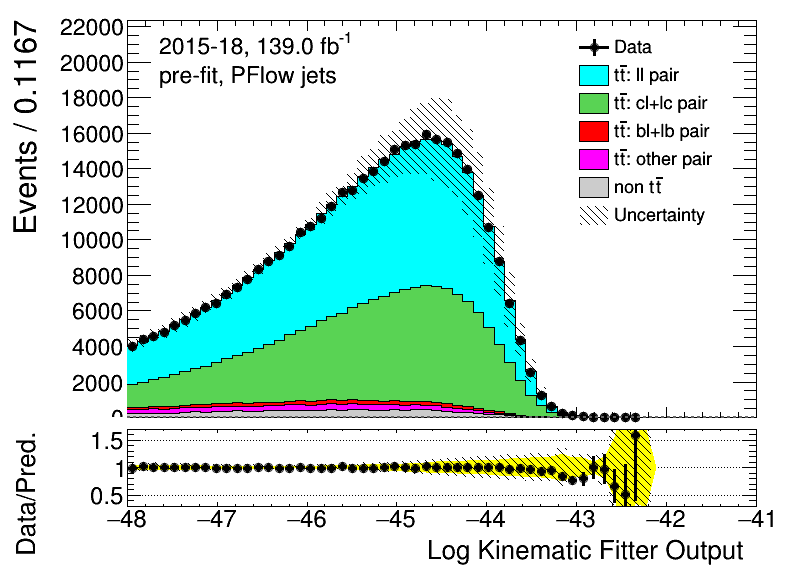
\includegraphics[width=0.45\textwidth]{FTAG_plots/pretagNoRwwithhighpTPFlowall/DataMC_h_LLR.png}
	\caption{Distribution of  the negative logarithm of the likelihood that
	is used to reconstruct the \ttbar\ decay.}
	\label{fig:llr}
\end{figure}
An additional requirement of log-likelihood > -48 is 
placed on the output of the likelihood value for the chosen event permutation. 
An example of the distribution of log-likelihood of the best permutations 
is shown in Figure~\ref{fig:llr}. 
In this figure, the data events are compared against the simulation.
The majority of the events come from \ttbar\ production. There is only
a very small fraction of events, which is denoted as ``non \ttbar''
on the figure, that come from other processes like $W$ or $Z$ production
in association with jets or single-top production.


\section{Event selection}
\label{Event selection}
 % The analysis uses the full available integrated luminosity collected with the ATLAS detector from the all years. This corresponds to a collected luminosity of 139 fb$^{-1}$. The event selection aims to select a sample enriched in $t\bar{t}$ events. The lowest un-prescaled single electron and single-muon triggers are used.
\subsection{Standard selection}
\label{standard selection}
Events are required to contain exactly one trigger-matched 
lepton with $p_{T} > 27$~GeV and exactly four jets with 
$p_{T} > 25$~GeV. Leptons are required to have $p_{T}$ 
above 27~GeV in order to avoid the turn-on curve for the 
single lepton triggers. Events which contain an additional 
lepton with $p_T > 27$~GeV are rejected. 
The events are also required to have $\MET > 20$~GeV, which is 
assumed to be the result of the neutrino from the leptonically 
decaying $W$ boson. The transverse
mass $m_T$ between the lepton and the \MET, is
constrained as follows:
\[ m_T = \sqrt{2 p_T^\ell \MET (1-\cos\Delta\phi)} > 40~\GeV,\]
where $\Delta\phi = \phi(\MET)-\phi(\ell)$ is the azimuthal difference between
the lepton and \MET.
\begin{table}[htb]
	\centering
	\small
	\setlength\tabcolsep{5pt} 
	\newcolumntype{C}{ @{}>{${}}c<{{}$}@{} }
	\begin{tabular}{|r *2{|rCr}| }
	\hline
	& \multicolumn{3}{|c|}{PFlow jets} & \multicolumn{3}{c|}{Track jets} \\
	\hline
	Data          &     227118       &   &              &   218351  &       &         \\  
	\ttbar\       &     235670       &\pm& 200          &   223770  &\pm& 180     \\
	Non \ttbar\   &     7610         &\pm& 120          &   7280    &\pm& 100    \\
	\hline
	Data/MC       &     0.934        &\pm& 0.002        &   0.945   &\pm& 0.002 \\
	\hline
	\end{tabular}
	\vspace{0.2cm}
	\caption{Standard selection: prefit comparison of the  number of events in data and in 
	simulation considering the PFlow jets and the VR-Track jets for 
	events with exactly 4 jets.}
	\label{tab:yields_standard}
\end{table}
\begin{figure}[bth]
	\centering
	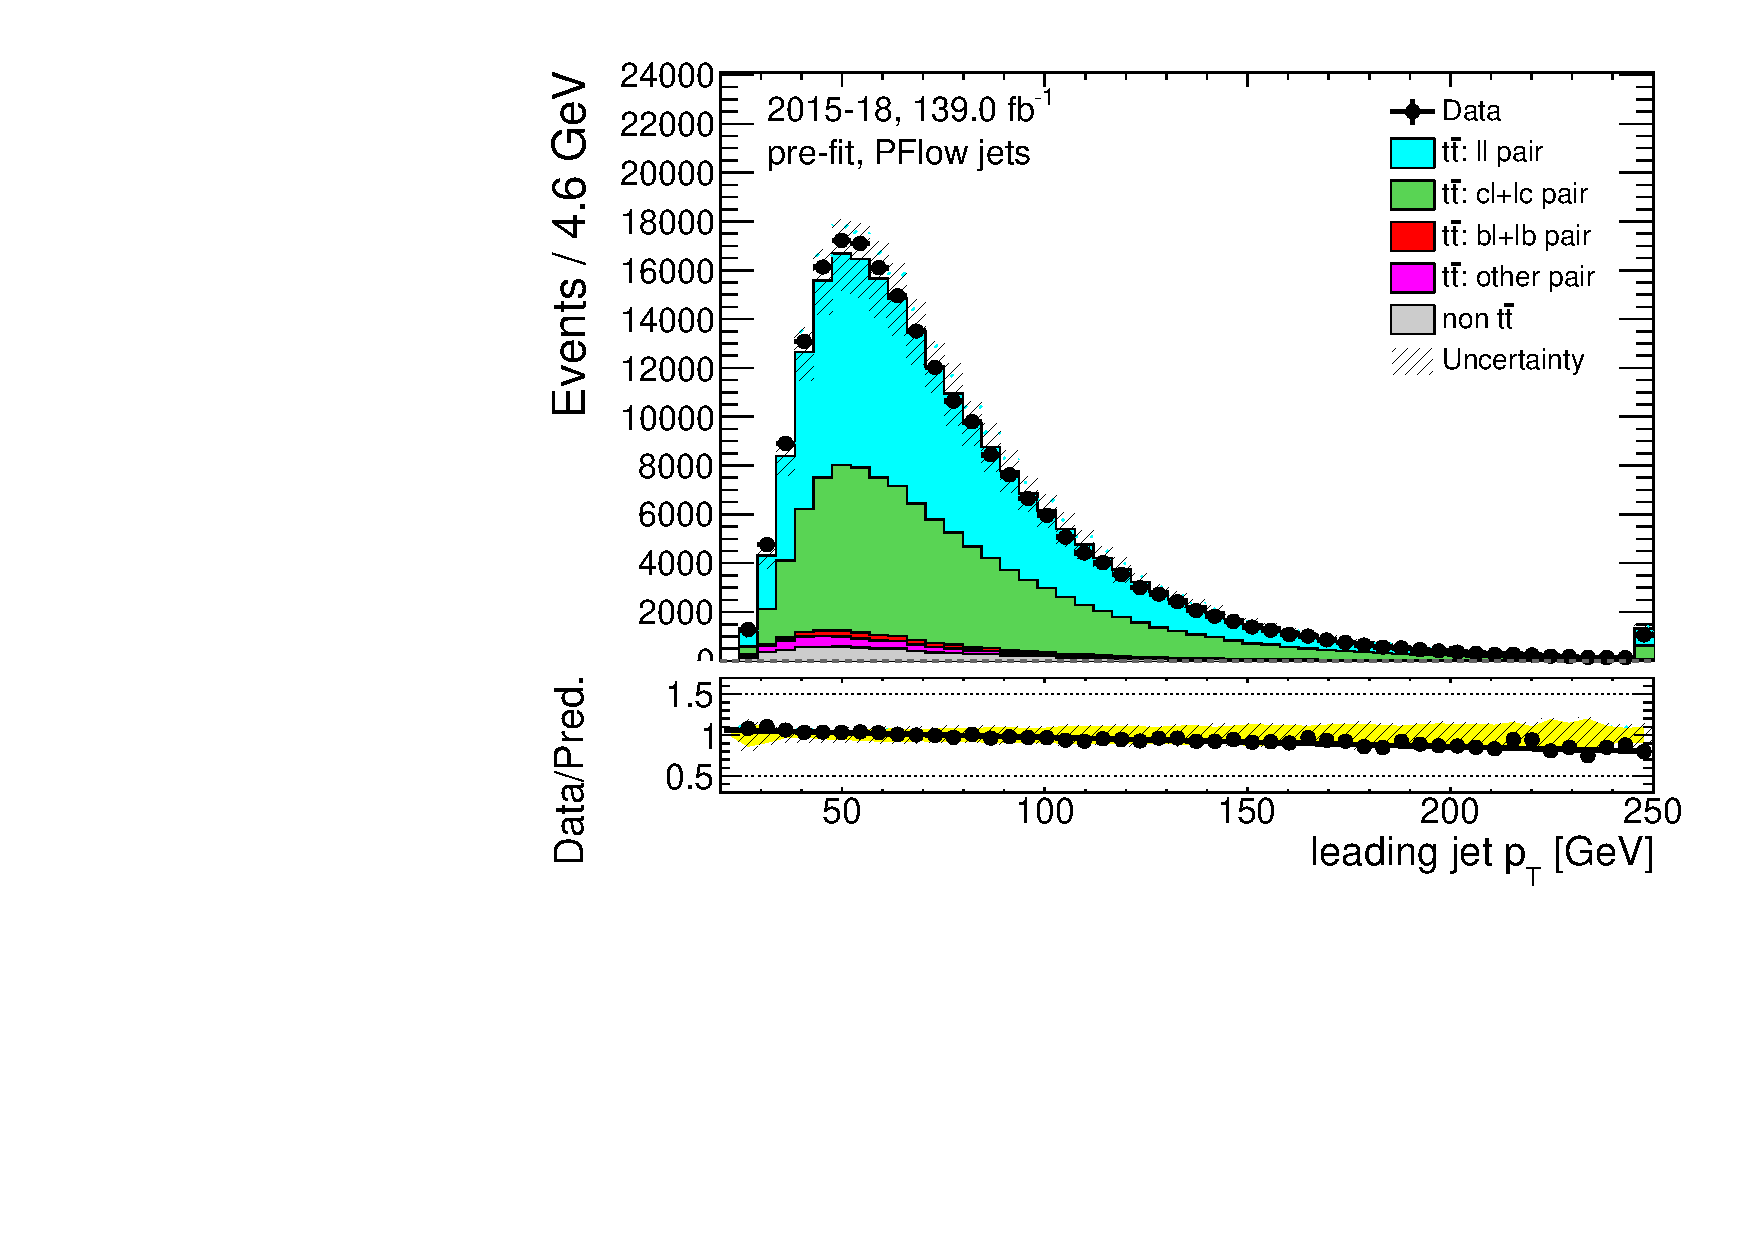
\includegraphics[width=0.45\textwidth]{FTAG_plots/pretagNoRwwithouthighpTPFlowall/DataMC_h_J0_pt.pdf}
	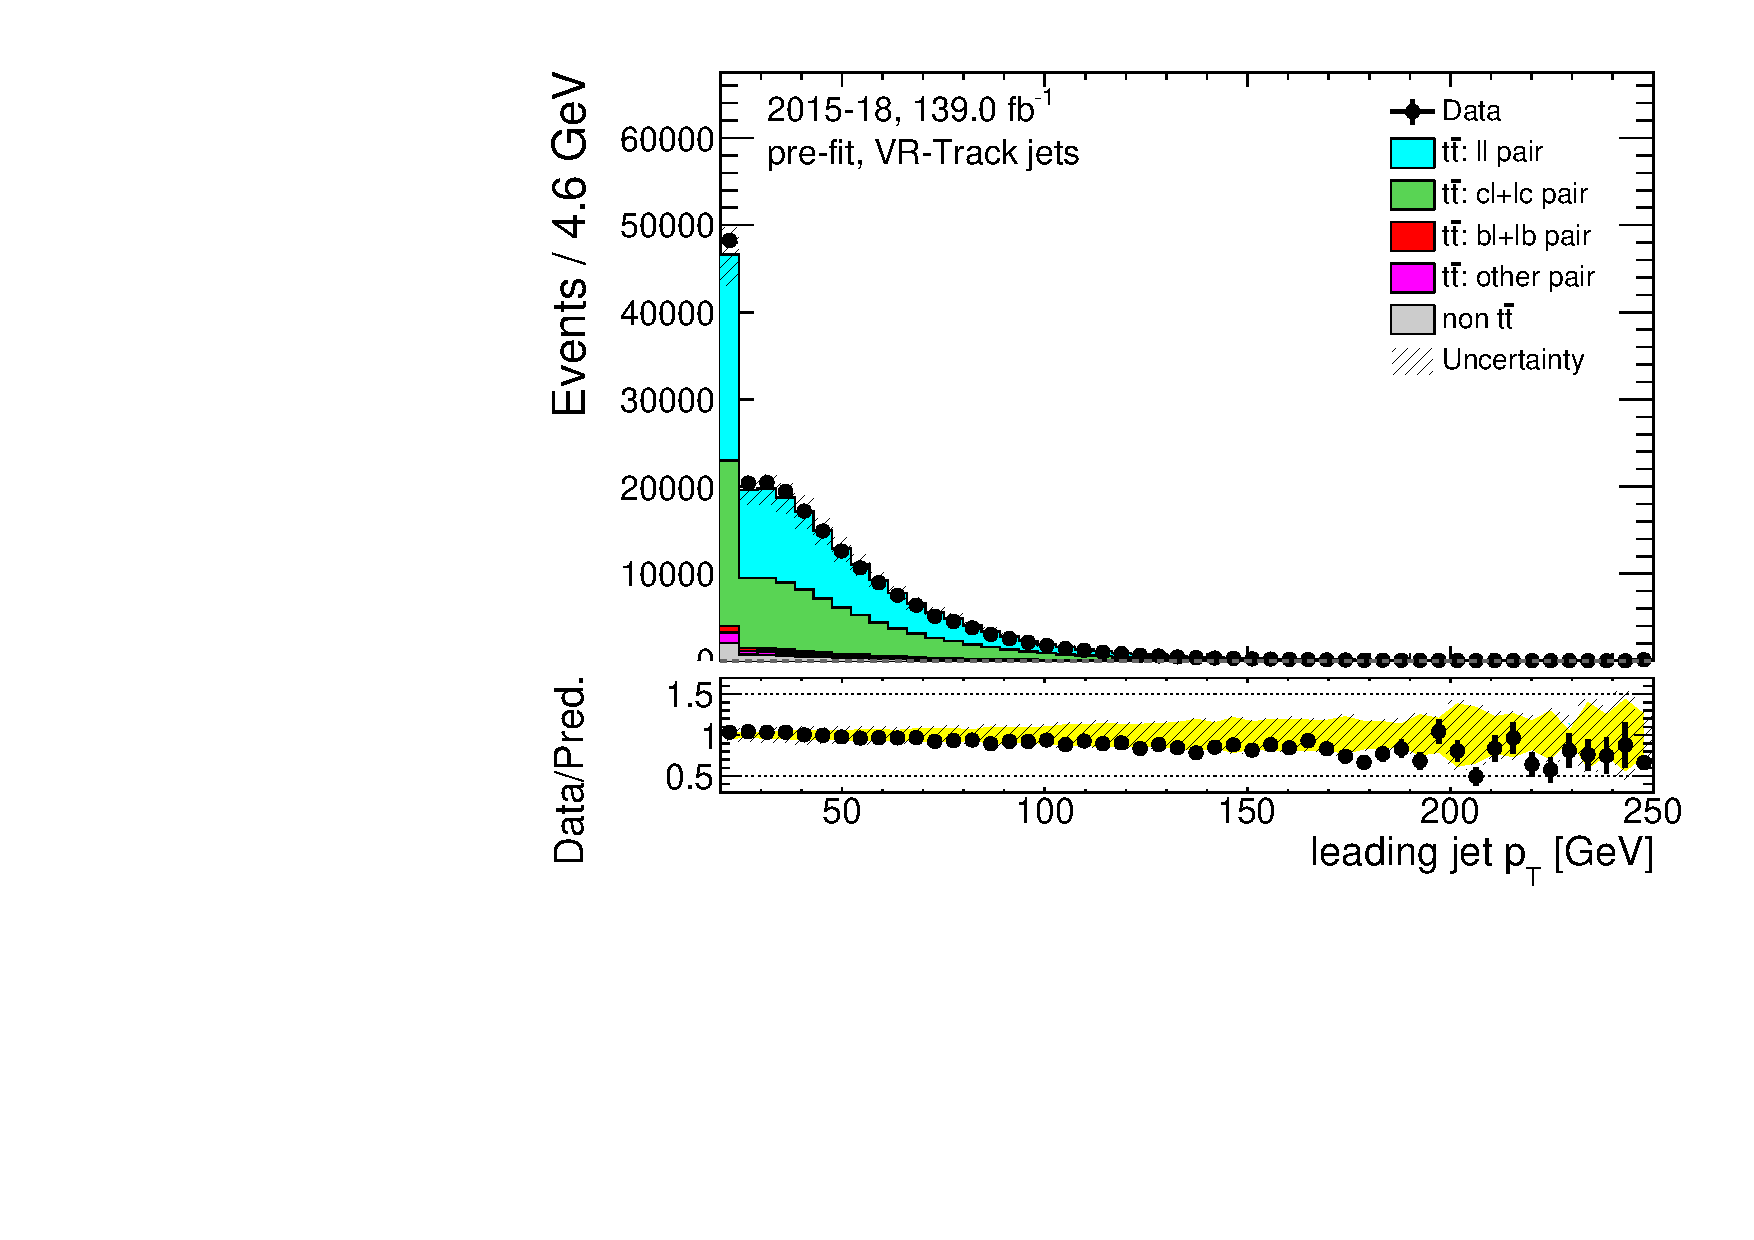
\includegraphics[width=0.45\textwidth]{FTAG_plots/pretagNoRwwithouthighpTVRJetsall/DataMC_h_J0_pttrackjet.pdf}\\
	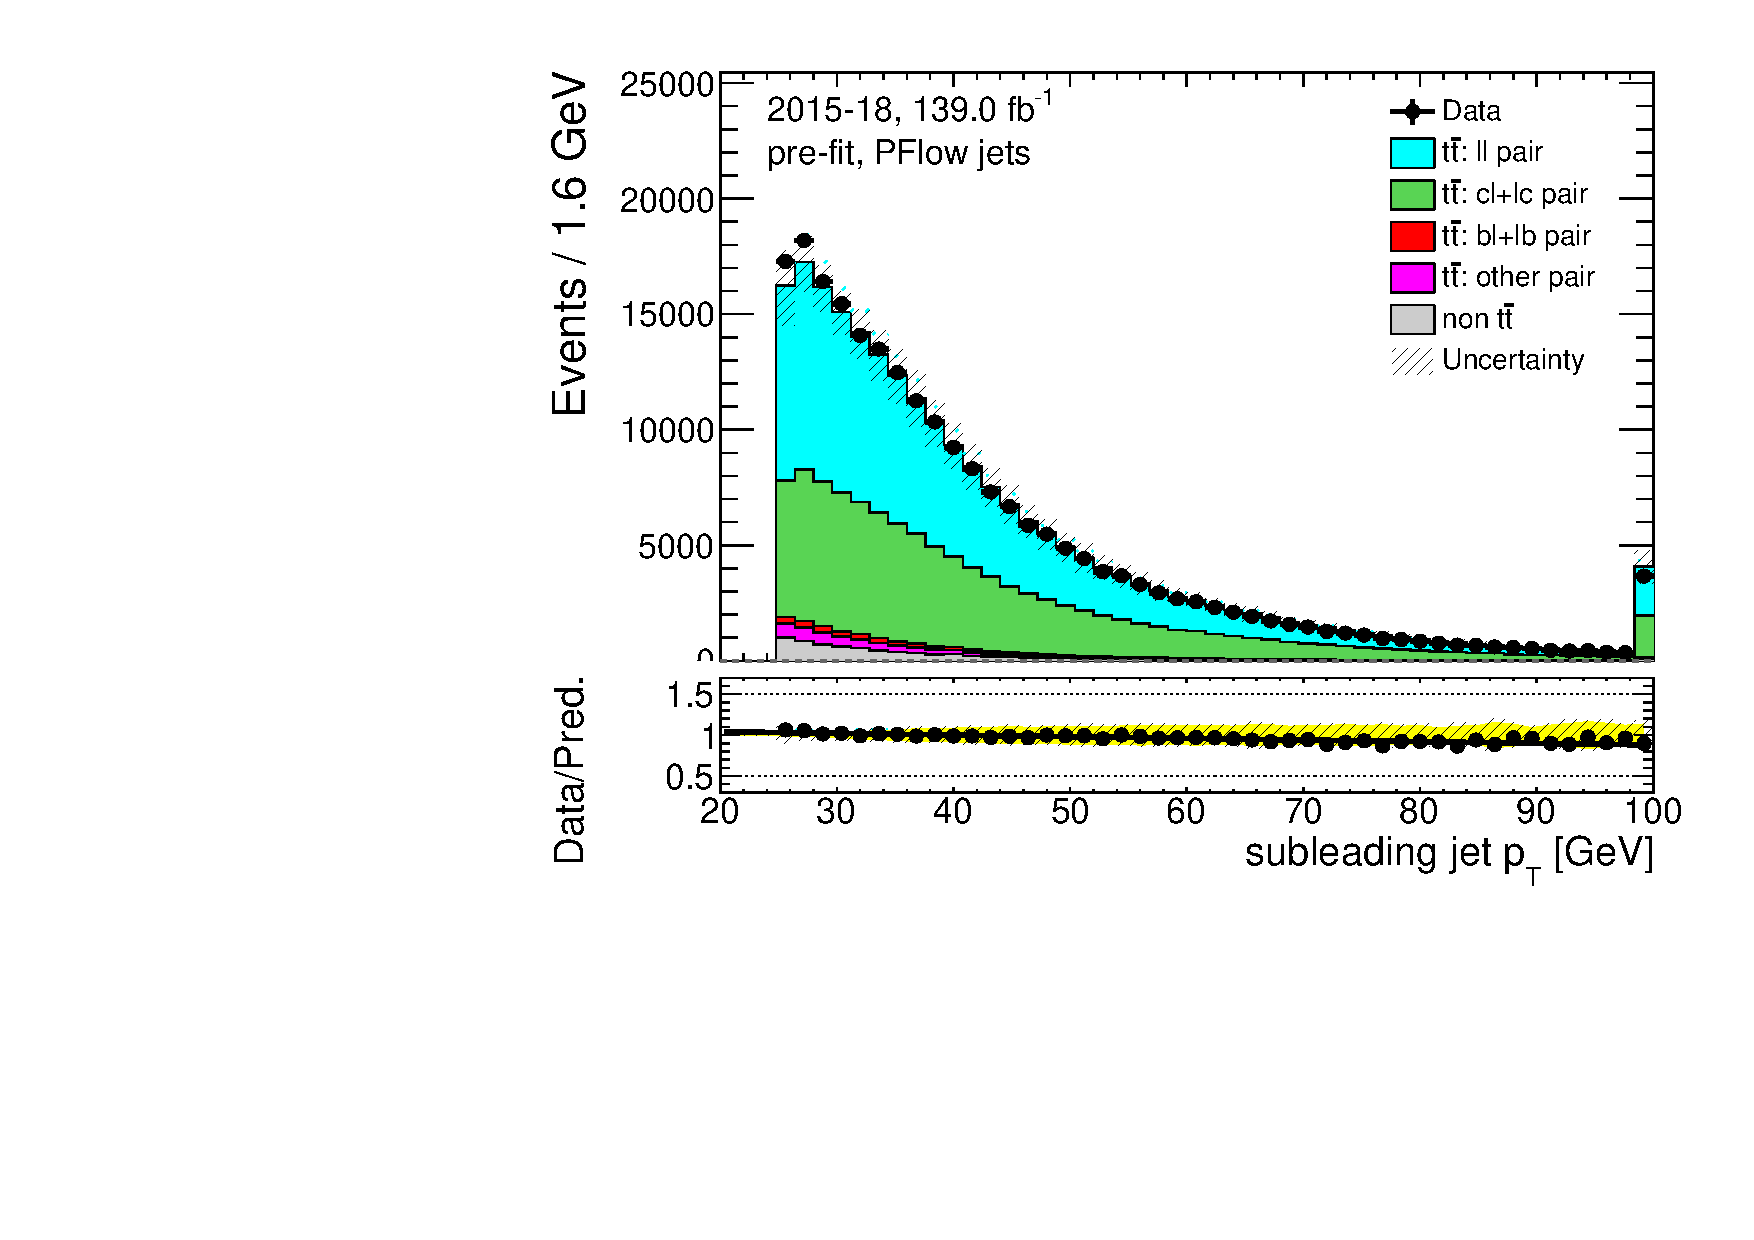
\includegraphics[width=0.45\textwidth]{FTAG_plots/pretagNoRwwithouthighpTPFlowall/DataMC_h_J1_pt.pdf}
	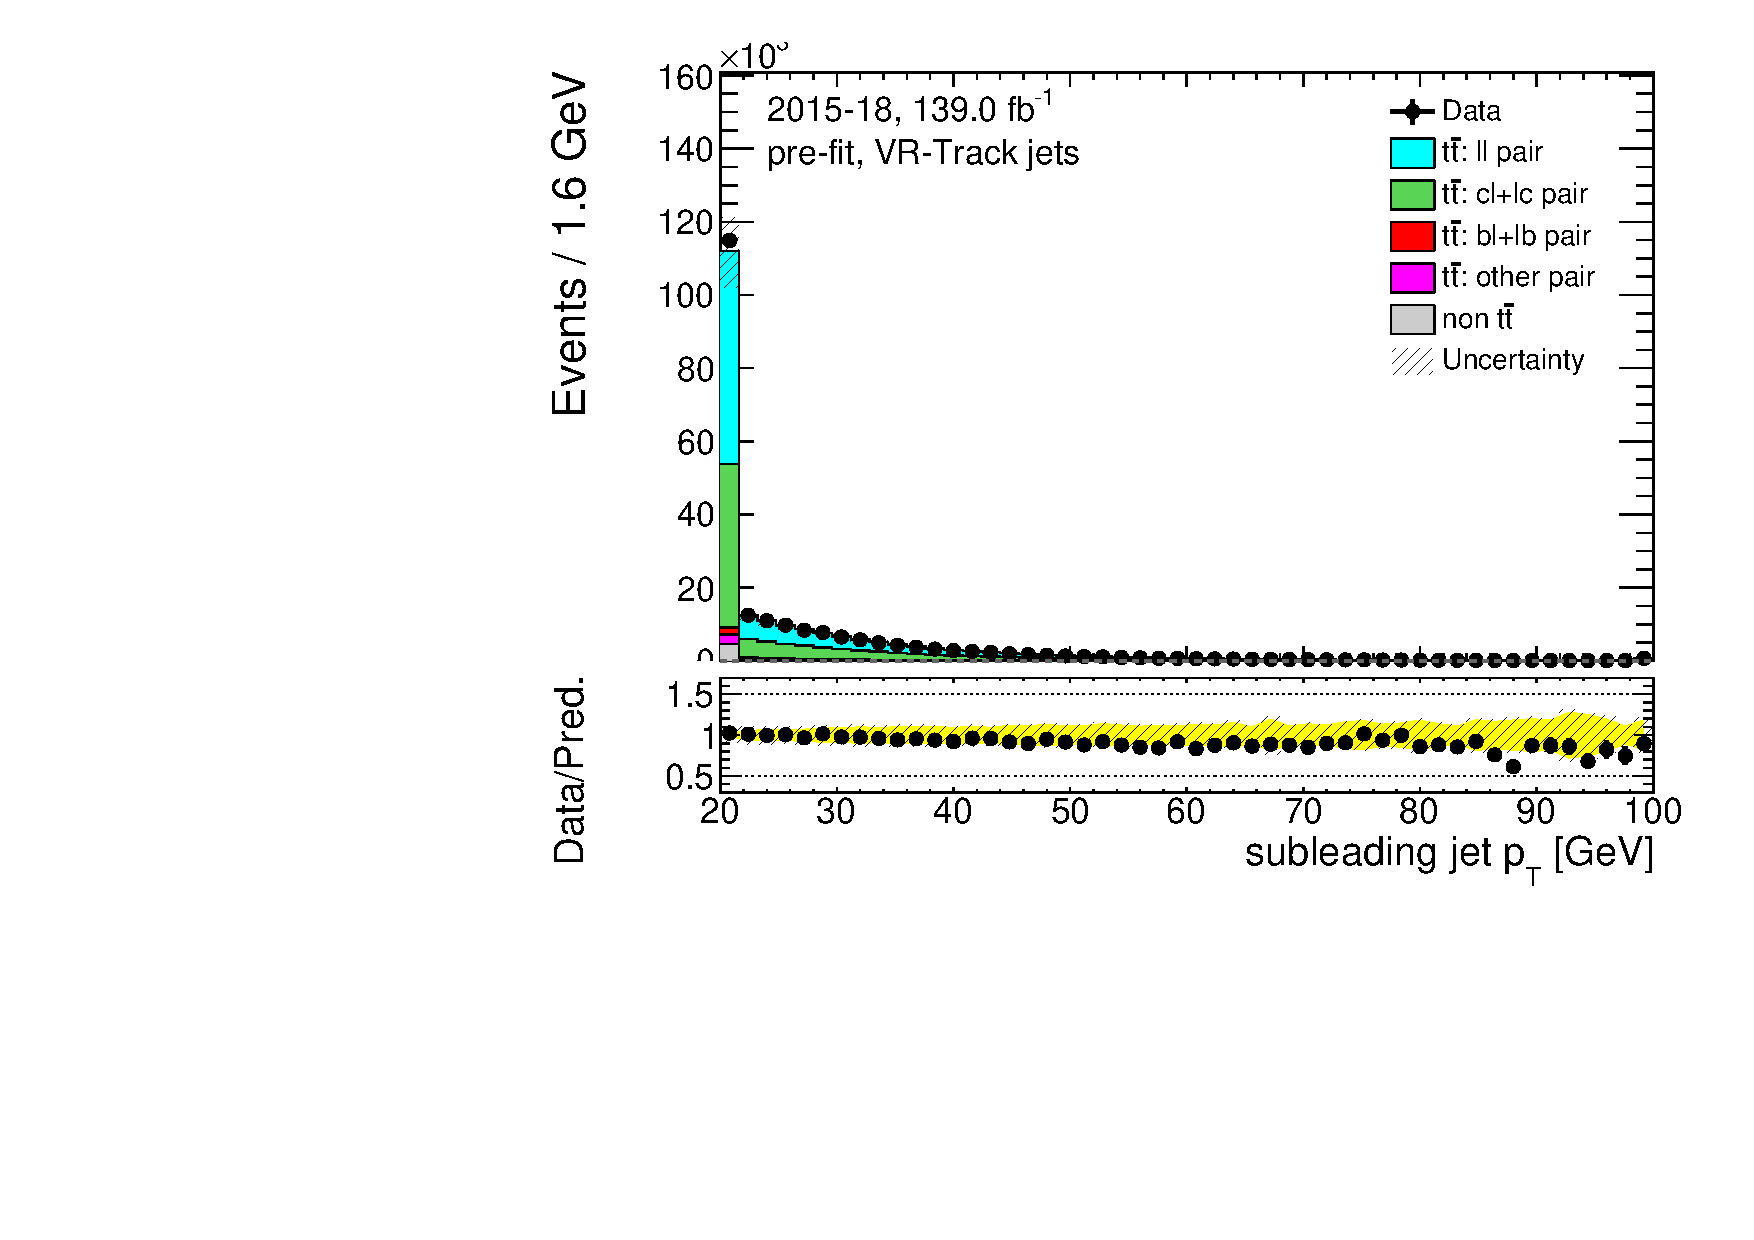
\includegraphics[width=0.45\textwidth]{FTAG_plots/pretagNoRwwithouthighpTVRJetsall/DataMC_h_J1_pttrackjet.pdf}\\
	\caption{Standard selection: data versus simulation of the leading and sub-leading $W$ jet \pt\ 
	for the PFlow jets in the left column and for VR-Track jets in the right column. 
	The leading jet and sub-leading jet refer to the highest \pt\ $W$ jet and the 
	second highest \pt\ jet, respectively. The 'non \ttbar' background 
	indicates background comes from non-\ttbar\ processes like $W$ or $Z$ production
	in association with jets or single-top production.
	The error in the table (and the following yields tables for
	different selection) is stats-only. }
	\label{fig:kinematic_distributions_standard}
\end{figure}
% Due to the requirement on jet $p_T$ and binning strategy, the calibration 
% result can be applied to jets with $p_{T}$ between 25 to 200~GeV. 
The yields of the data and the MC are given in Table \ref{tab:yields_standard}.
An example of the \pt\ distributions
before any tagging or fitting and 
after the standard selection is shown in Figure~\ref{fig:kinematic_distributions_standard}. 
More plots can be found in Appendix \ref{sec:appendix_standard_selection}.
The yellow band in the lower pad shows the overall systematic uncertainties, combining the 
experimental uncertainties and the \ttbar\ modelling uncertainties, as described in 
Section \ref{sec:FTAG_systematics}. The data/MC ratio shows good agreement 
within the systematic uncertainties. 

\subsection{Low-\pt\ selection}
\label{sec:lowpT_selection}
The author has developed an othorgonal selection to 
extend the calibration in the low-$p_{T}$ region so that the calibration 
can be applied to PFlow jets with $20< \pt\ < 25$~GeV.
The \pt\ threshold of the VR-Track jets is $10$~GeV 
therefore the low-\pt\ selection is not needed. 
Instead of requiring events to 
have exactly 4 jets $\pt\ > 25$~GeV, events are required to have exactly 3 jets with $p_{T} > 25$~GeV 
and exactly 1 jet with $25$~GeV $> p_{T} > 20$~GeV. Other than that, 
all requirements for the selection are the same. 
This additional cut provides candidates for the PFlow $W$ jet that is used 
for calibration in the $20-25$~GeV region. 
The inclusive yields of the low-\pt\ selection 
of the data and the MC are given in Table \ref{tab:yields_lowpT}, and
the \pt\ distributions of the $W$ jets are shown in Figure~\ref{fig:kinematic_distributions_lowpT}.
More plots of the kinematic distributions
are shown in Appendix \ref{sec:appendix_lowpT_selection}. 
Good agreement between MC and data 
is shown in these distributions, and the $p_{T}$ range of the sub-leading has gone down to 20~GeV. 


\begin{table}[bht]
	\centering
	\small
	\setlength\tabcolsep{5pt} 
	\newcolumntype{C}{ @{}>{${}}c<{{}$}@{} }
	\begin{tabular}{|r *1{|rCr}| }
	\hline
	& \multicolumn{3}{|c|}{PFlow jets} \\
	\hline
	Data          &     59987       &   &                      \\  
	\ttbar\       &     56530       &\pm&     90        		 \\
	Non \ttbar\   &     3340        &\pm&     60    		 \\
	\hline
	Data/MC       &     1.002       &\pm&  0.004      			 \\
	\hline
	\end{tabular}
	\vspace{0.2cm}
	\caption{Low-\pt\ selection: prefit comparison 
	of the number of events in data and MC 
	for the PFlow $W$ jets. Events are required to have 
	exactly 3 jets with $\pt\ > 25$~GeV 
	and one jet with $20 < \pt\ < 25$~GeV.}
	\label{tab:yields_lowpT}
\end{table}

\begin{figure}[H]
	\centering
	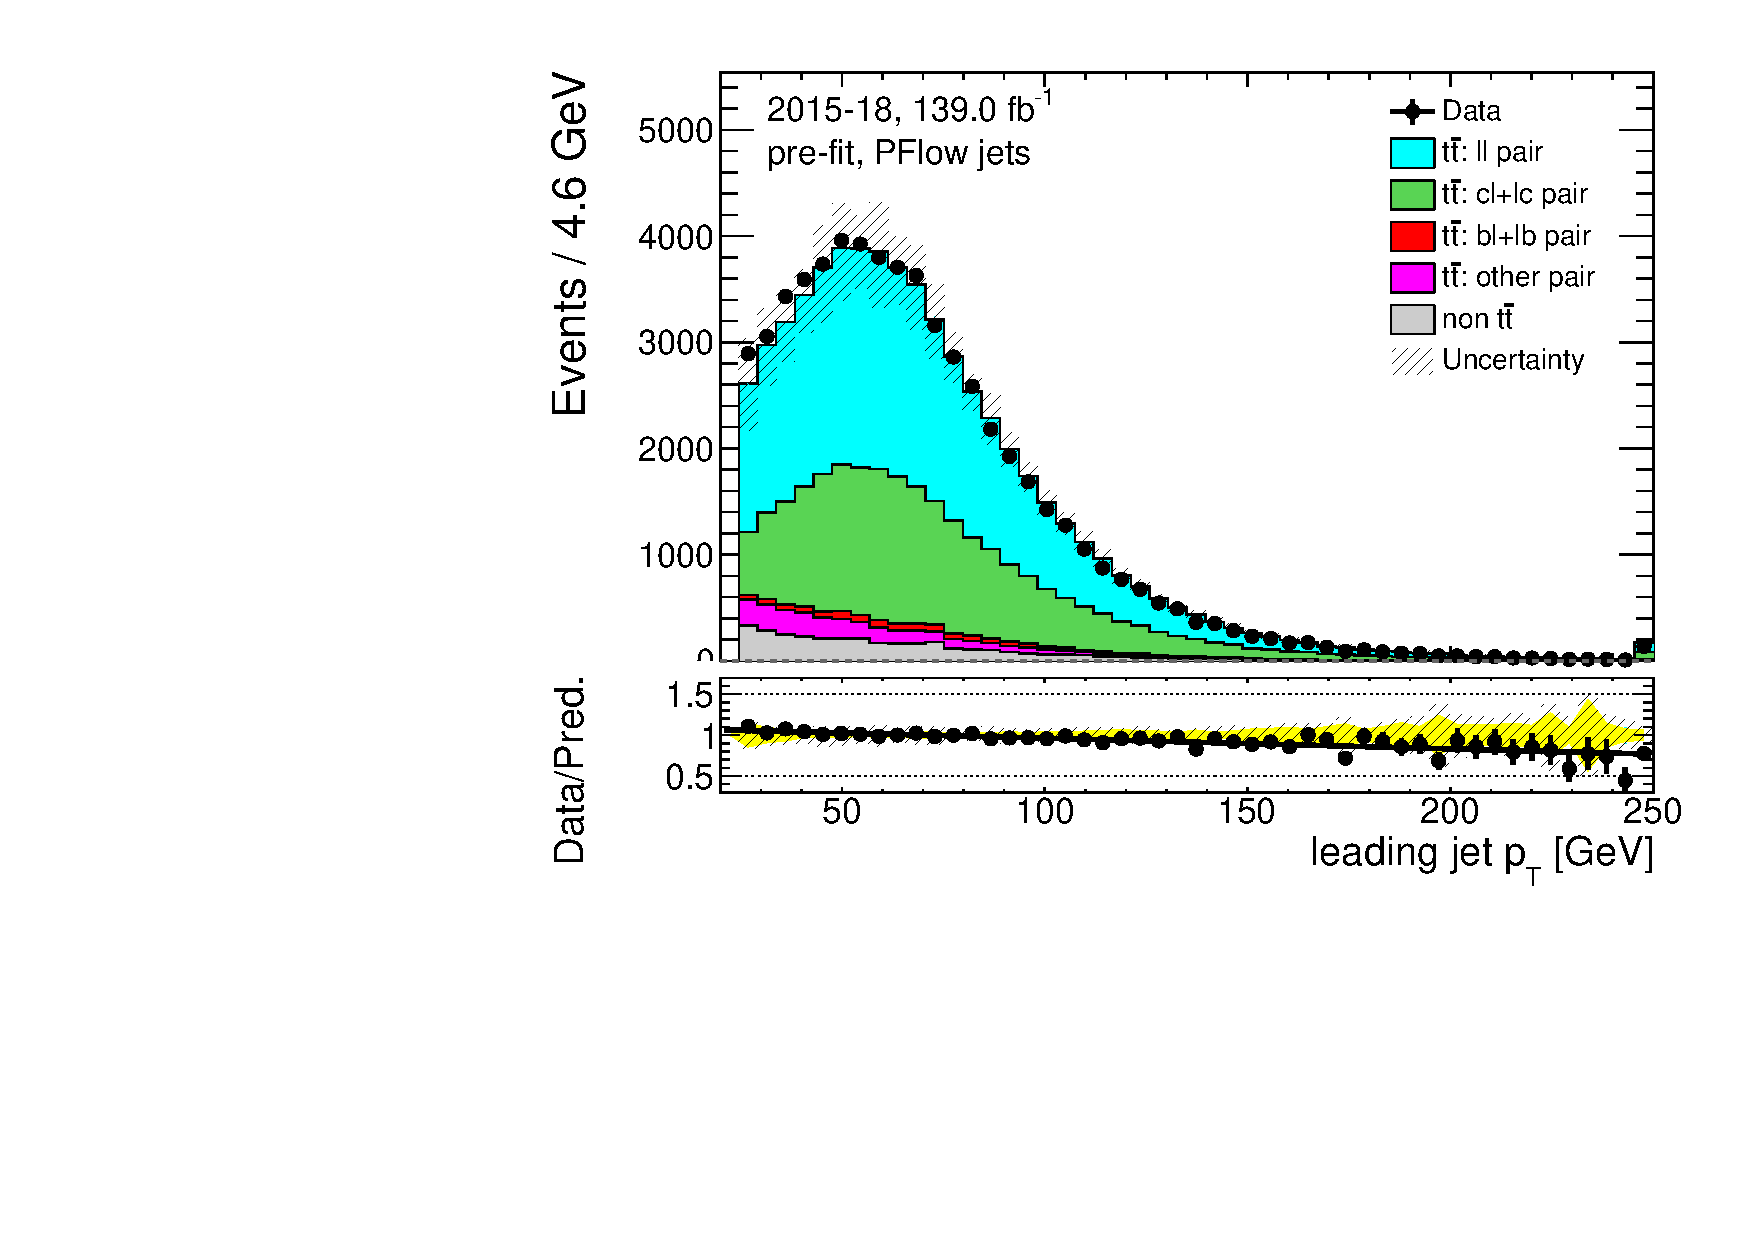
\includegraphics[width=0.45\textwidth]{FTAG_plots/pretagNoRwLowpTPFlowall/DataMC_h_J0_pt.pdf}
	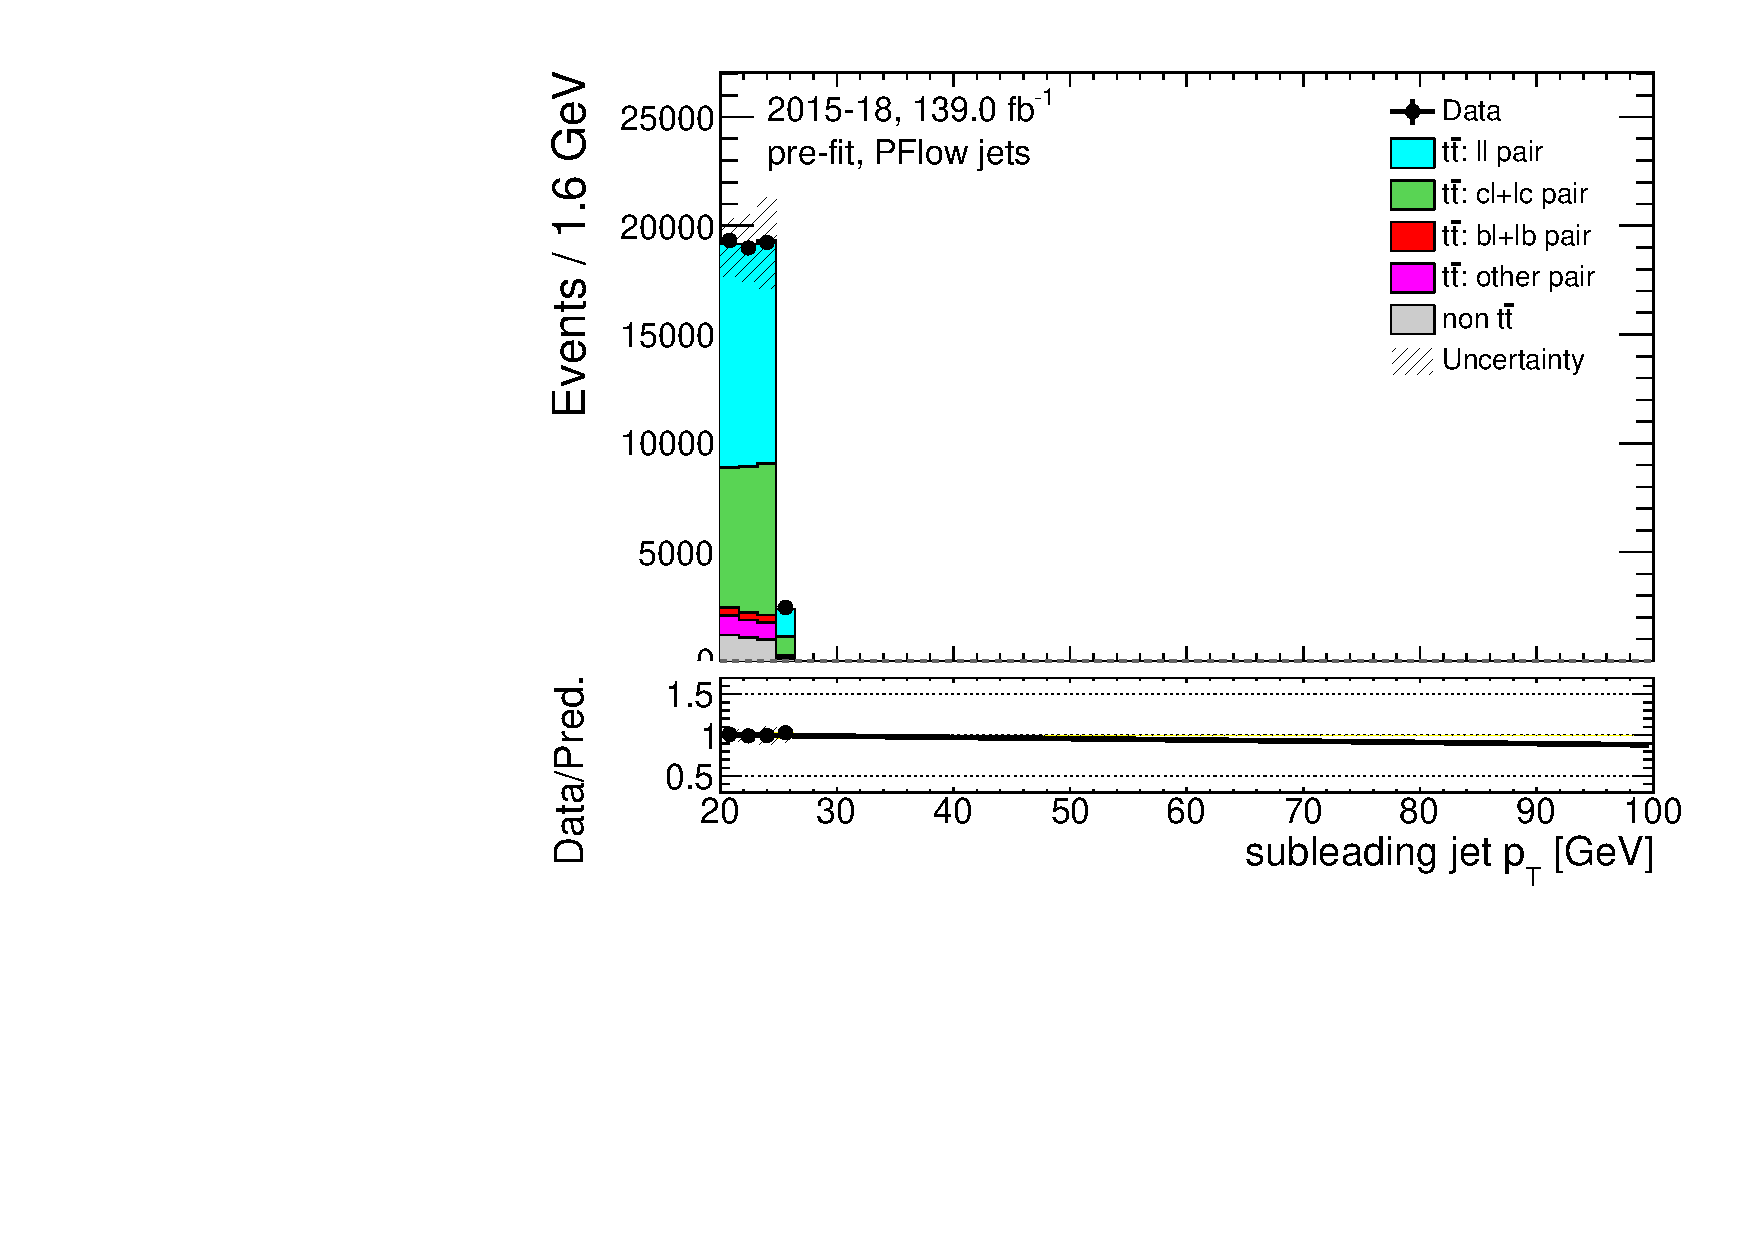
\includegraphics[width=0.45\textwidth]{FTAG_plots/pretagNoRwLowpTPFlowall/DataMC_h_J1_pt.pdf}\\
	\caption{Low-\pt\ selection: data versus simulation of the 
	PFlow $W$ jets \pt. }
	\label{fig:kinematic_distributions_lowpT}
\end{figure}


\subsection{High-$p_T$ selection}
\label{high_pt_selection}
It has been observed that in the previous calibrations that the statistics 
are relatively low for the high-\pt\ region (e.g.\ jet $\pt\ > 100$~GeV). 
Therefore, the author has worked on an othorgonal selection to improve this situation.
Instead of requiring events to have exactly 4 jets, events are required to 
have at least 5 jets with $p_{T} > 25$~GeV, in which at least 
1 jet with $\pt\ > 70$~GeV. Other than that, all 
requirements for the selection remain the same. 


The choice of cut value at $70$~GeV is based on the
study shown in the following. 
The effect on the \cjet\ purity and the potential statistical gain is investigated, 
where the \cjet\ purity is defined as:
\begin{equation}
\cjetineq\ \rm{purity} = \frac{N_{\rm{true}\ \cjetunder}}{N_{\rm{all}}},
\end{equation}
where $N_{\rm{true}\ \cjetunder}$ stands for the number of events with a 
true \cjet\ from the $W$ decay, and $N_{\rm{all}}$ stands for the number of all events. 
The ideal situation is the high-\pt\ selection will maximally increase the 
statistics while mininally decreasing the \cjet\ purity, therefore a figure of merit $P^{\rm{Cut}}$
is defined as:
\[P^{\rm{Cut}} = \frac{\sum_i{\rm{Gain\ in\ stats}^2_i}}{\sum_i{\cjetineq \rm{purity}^2_i }}, \]
where i stands for the number of bins. The ``Gain in stats'' stands for increase in 
statistics and it's summed over all bins in Figure~\ref{fig:cutvalue}.
The \cjet\ purity and the statistical gain are calculated for 4 different cut 
values as shown in Figure~\ref{fig:cutvalue}, comparing with the cut value of 0. 
The value of $70$~GeV is chosen as it gives the highest value of $P^{\rm{Cut}}$. 


\begin{figure}[bth]
	\centering
	\begin{subfigure}[t]{.38\linewidth}
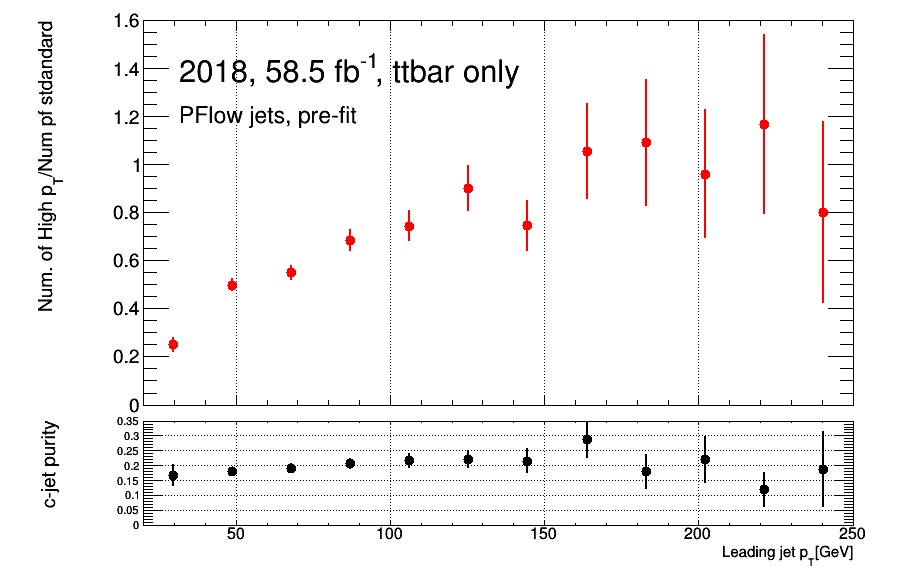
\includegraphics[width=1\textwidth]{FTAG_plots/stat_gains/statsgain_0GeV.png}
\caption{No cut}
\end{subfigure}
\begin{subfigure}[t]{.38\linewidth}
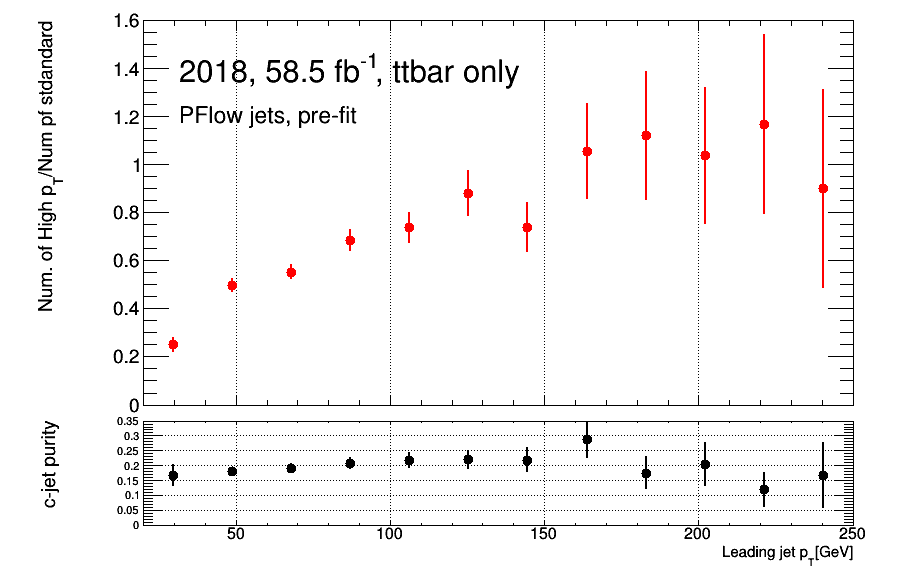
\includegraphics[width=1\textwidth]{FTAG_plots/stat_gains/statsgain_40GeV.png}
\caption{Cut value: 40~GeV}
\end{subfigure}
\begin{subfigure}[t]{.38\linewidth}
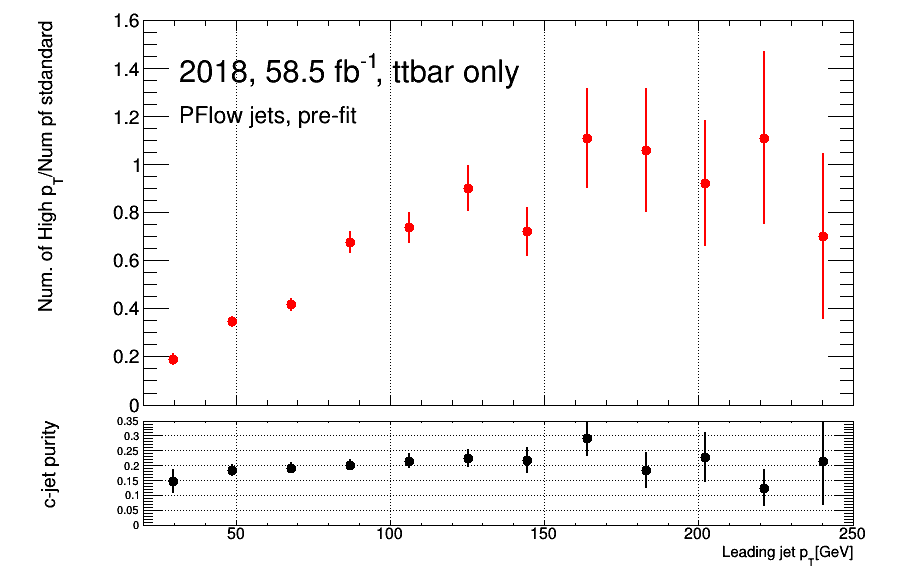
\includegraphics[width=1\textwidth]{FTAG_plots/stat_gains/statsgain_70GeV.png}
\caption{Cut value: 70~GeV}
\end{subfigure}
\begin{subfigure}[t]{.38\linewidth}
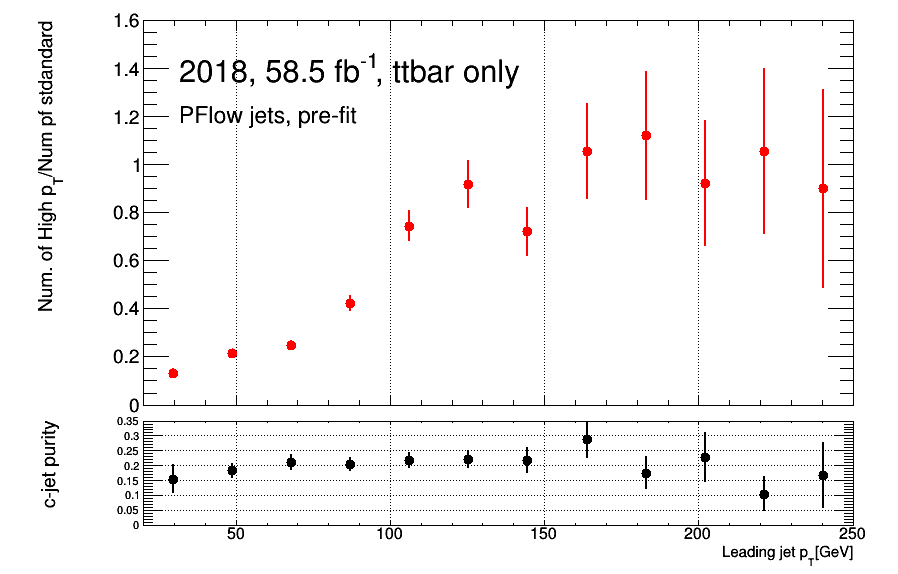
\includegraphics[width=1\textwidth]{FTAG_plots/stat_gains/statsgain_90GeV.png}
\caption{Cut value: 90~GeV}
\end{subfigure}
\begin{subfigure}[t]{.38\linewidth}
\centering
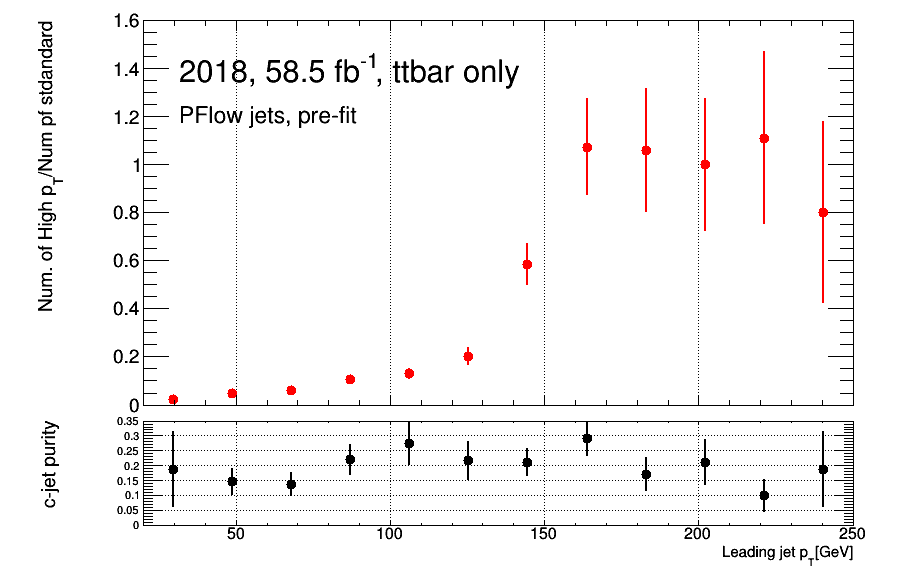
\includegraphics[width=1\textwidth]{FTAG_plots/stat_gains/statsgain_140GeV.png}
\caption{Cut value: 140~GeV}
\end{subfigure}

\caption{Comparison of different cut values in terms of gain in stats and \cjet\ purity.}
\label{fig:cutvalue}
\end{figure}

\begin{table}[ht]
	\centering
	\small
	\setlength\tabcolsep{5pt} 
	\newcolumntype{C}{ @{}>{${}}c<{{}$}@{} }
	\begin{tabular}{|r *2{|rCr}| }
	\hline
	& \multicolumn{3}{|c|}{PFlow jets} & \multicolumn{3}{c|}{Track jets} \\
	\hline
	
	Data    &     98273  &           &   &        83957   &              &   \\ 
	\ttbar\ &    99430 &\pm&  120 &        87476 &\pm&  110     \\
	Non \ttbar\   &      1842  &\pm&  21 &          1570  &\pm&  20     \\
	\hline
	Data/MC &      0.97  &\pm&  0.003   &     0.94  &\pm&  0.003       \\
	\hline

	\end{tabular}
	\vspace{0.2cm}
	\caption{High-\pt\ selection: prefit comparison of the number of events in data and in 
	simulation considering the PFlow $W$ jets and the VR-Track jets.}
	\label{tab:yields_highpT}
	\end{table}

\begin{figure}[bth]
	\centering
	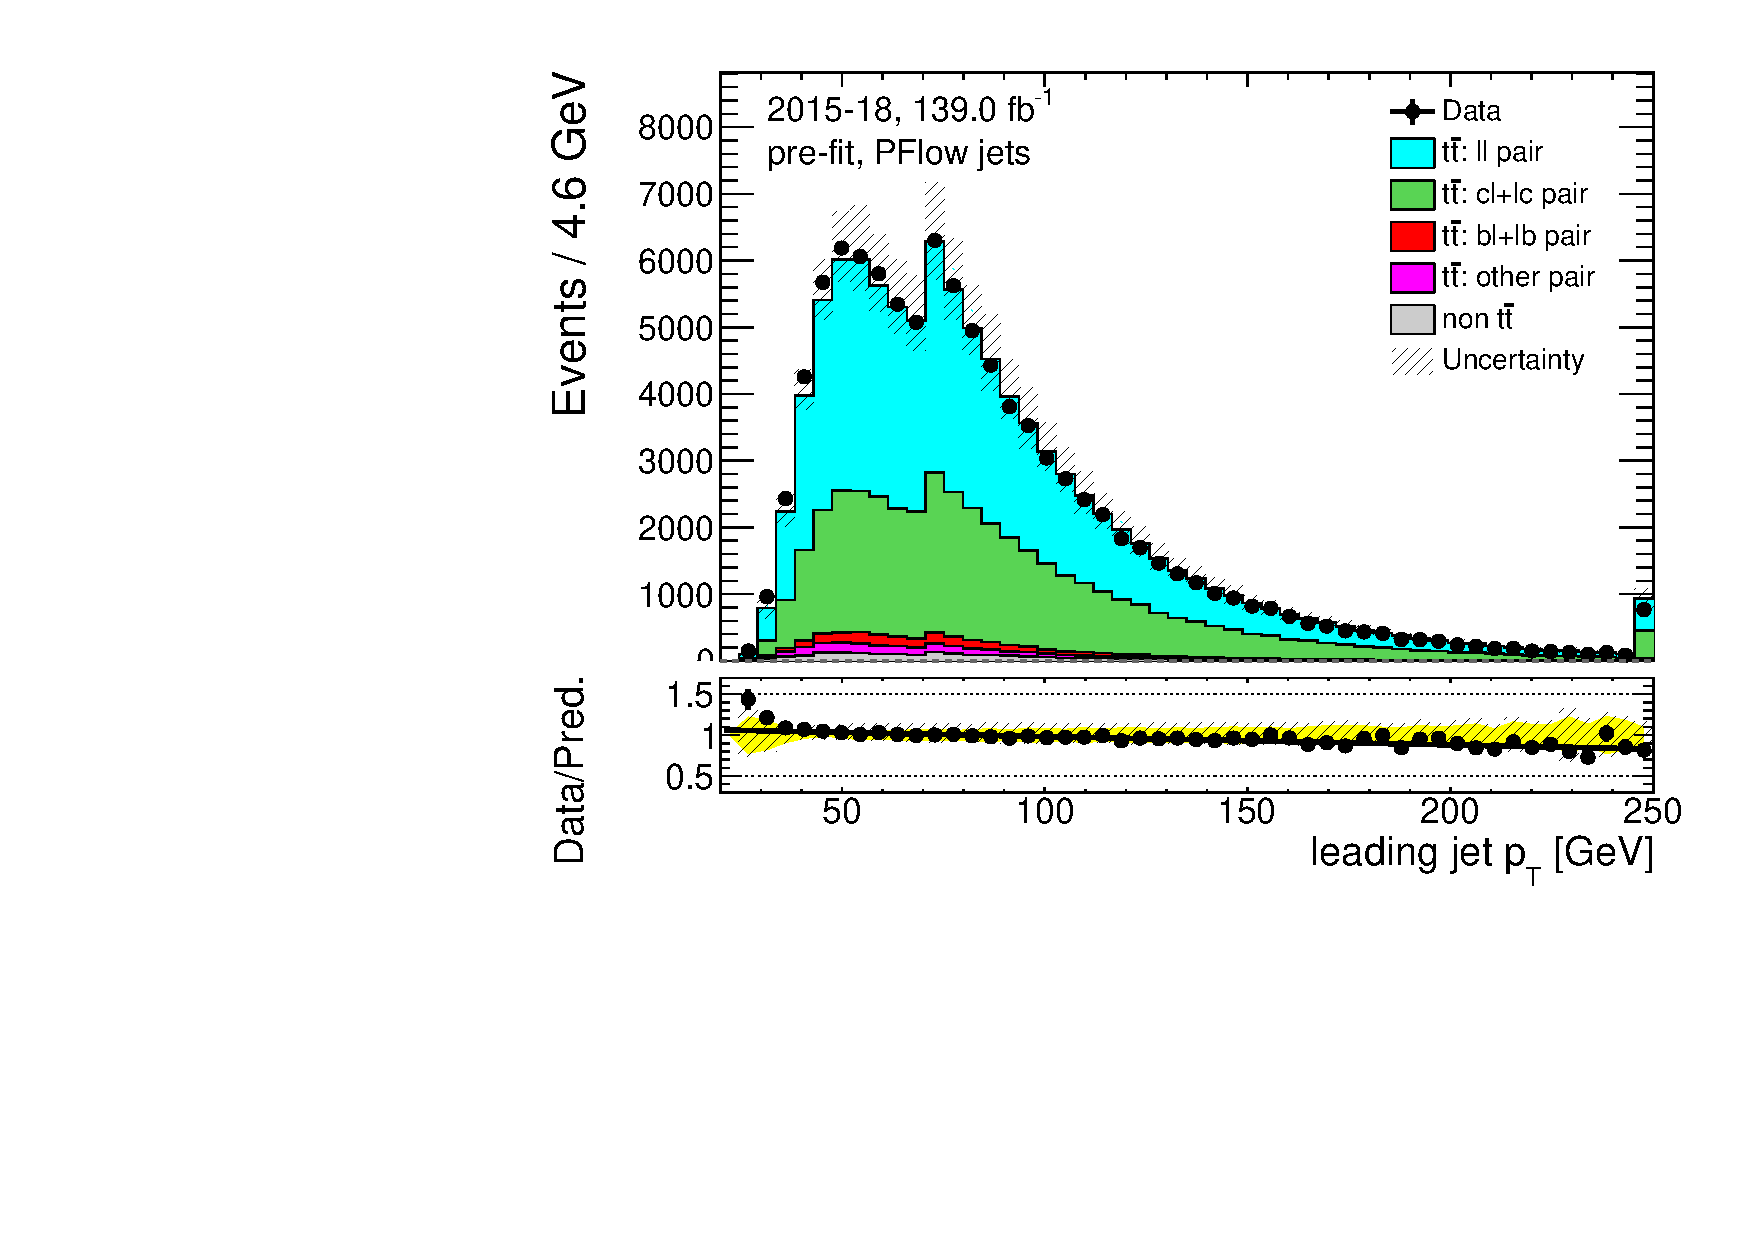
\includegraphics[width=0.45\textwidth]{FTAG_plots/pretagNoRwnewonlyPFlowall/DataMC_h_J0_pt.pdf}
	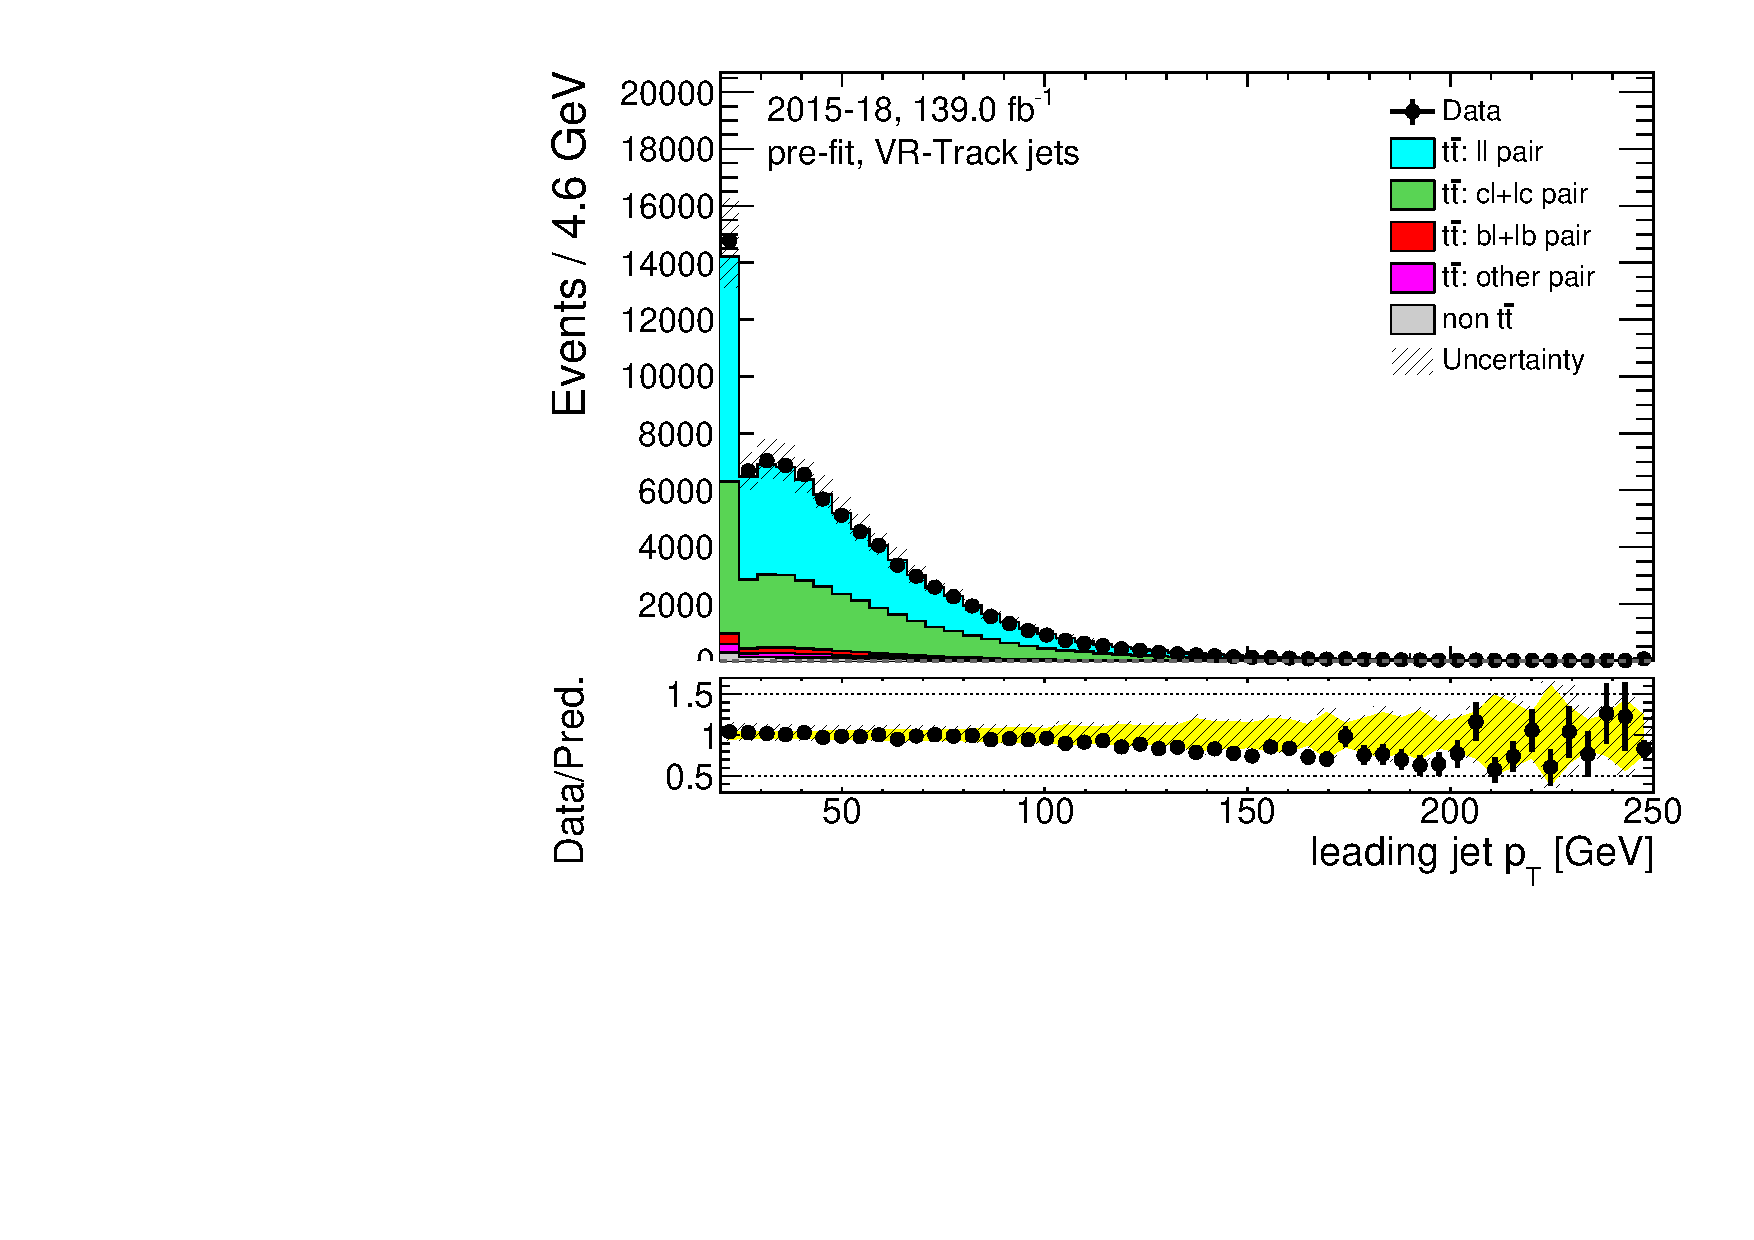
\includegraphics[width=0.45\textwidth]{FTAG_plots/pretagNoRwnewonlyVRJetsall/DataMC_h_J0_pttrackjet.pdf}\\
	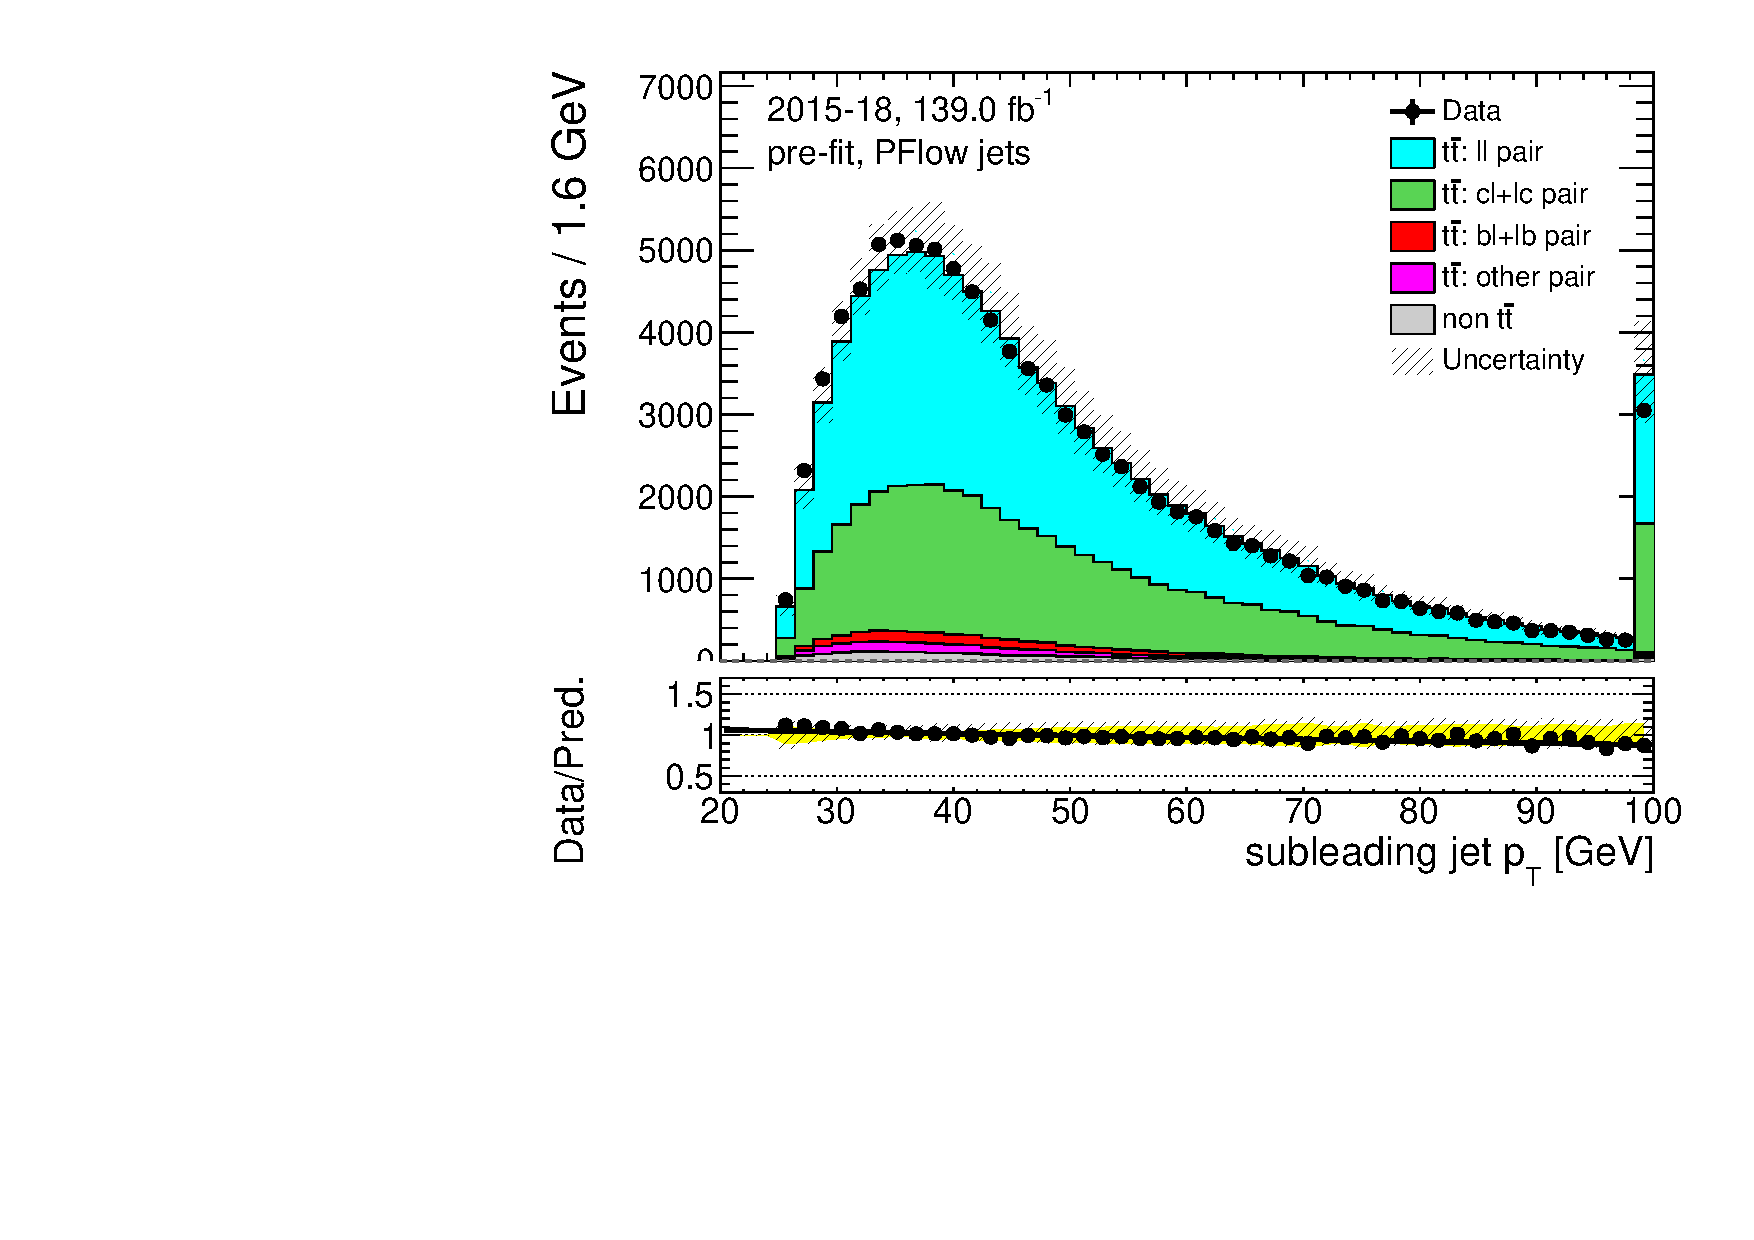
\includegraphics[width=0.45\textwidth]{FTAG_plots/pretagNoRwnewonlyPFlowall/DataMC_h_J1_pt.pdf}
	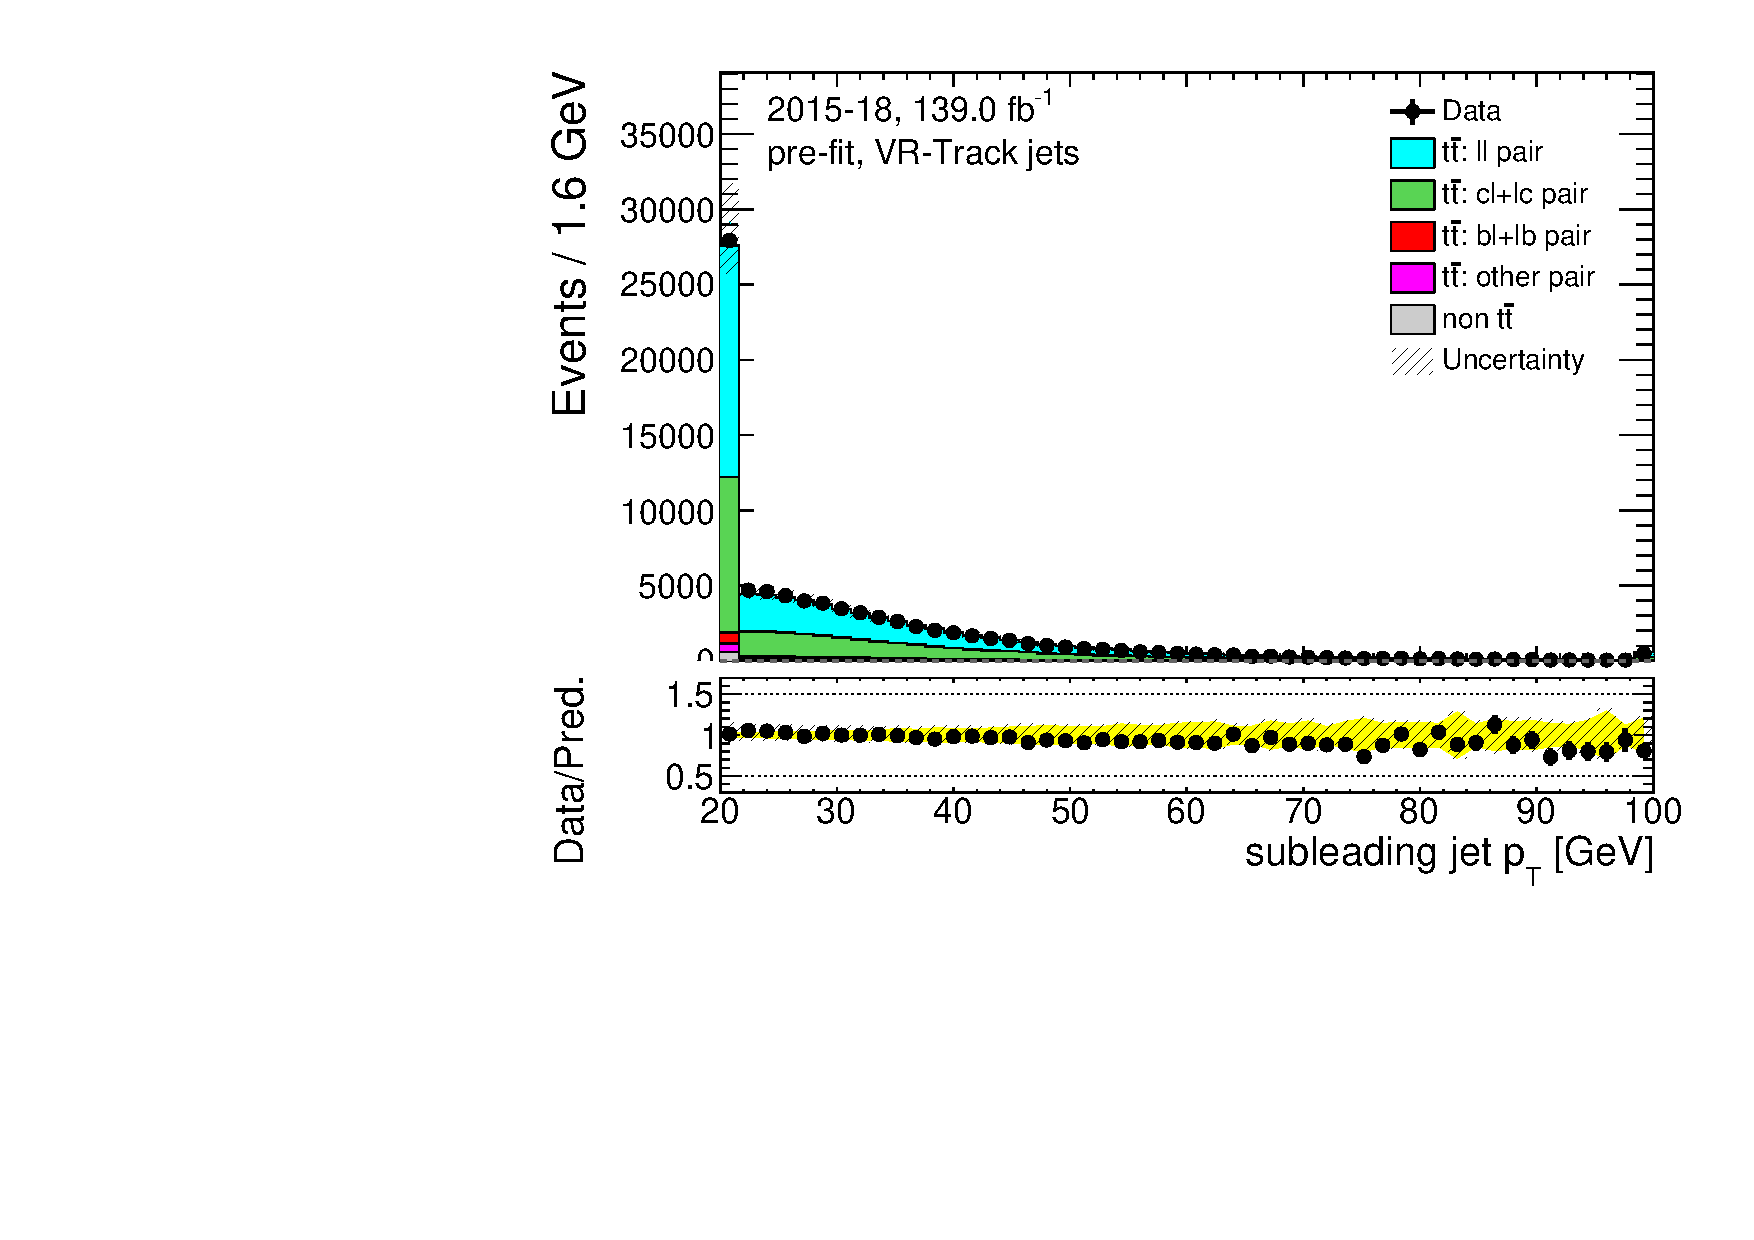
\includegraphics[width=0.45\textwidth]{FTAG_plots/pretagNoRwnewonlyVRJetsall/DataMC_h_J1_pttrackjet.pdf}\\
	\caption{High-\pt\ selection: data versus simulation of $W$ jets \pt\ for 
	PFlow jets in the left column and for VR-Track jets in the right column.}
	\label{fig:kinematic_distributions_highpT}
\end{figure}
	

The yields of the data and the MC are given in Table \ref{tab:yields_highpT}. 
An example of the \pt\ distributions before any tagging or fitting, applying 
the high-\pt\ selection is shown in Figure~\ref{fig:kinematic_distributions_highpT}. 
In general the event statistics improve about 80\% in region with \pt\ > 70~GeV as desired.
More plots can be found in Appendix \ref{sec:appendix_highpT_selection}.




\subsection{Combined selection}
\label{combined_selection}
As the standard selections, low-\pt\ selection and high-\pt\ selection are othorgonal 
to each other, all the selections are combined to provide the maximum range 
and statistics for the calibration. 
The yields of the data and the MC are given in Table \ref{tab:yields_combined}, 
an example of the \pt\ distributions before any tagging or fitting and 
after the combined selection is shown in Figure~\ref{fig:kinematic_distributions_combined}. More plots 
can be found in Appendix \ref{sec:appendix_combined_selection}.

\begin{table}[ht]
	\centering
	\small
	\setlength\tabcolsep{5pt} 
	\newcolumntype{C}{ @{}>{${}}c<{{}$}@{} }
	\begin{tabular}{|r *2{|rCr}| }
	\hline
	& \multicolumn{3}{|c|}{PFlow jets} & \multicolumn{3}{c|}{Track jets} \\
	\hline
	Data          &    385378           &      &        &   302308         &  &     \\  
	\ttbar\       &      383520   &\pm&  230 &            302690 &\pm&  200   \\
	Non \ttbar\         &        12420  &\pm&  120 &             8570  &\pm&  100     \\
	Data/MC       &        0.973  &\pm&  0.002 &           0.971 &\pm&  0.002          \\
	\hline

	\end{tabular}
	\vspace{0.2cm}
	\caption{Combined selection: prefit comparison of the number of events in data and in 
	simulation considering the PFlow jets and the VR-Track jets for an inclusive
	selection.}
	\label{tab:yields_combined}
	\end{table}

\begin{figure}[bth]
		\centering
		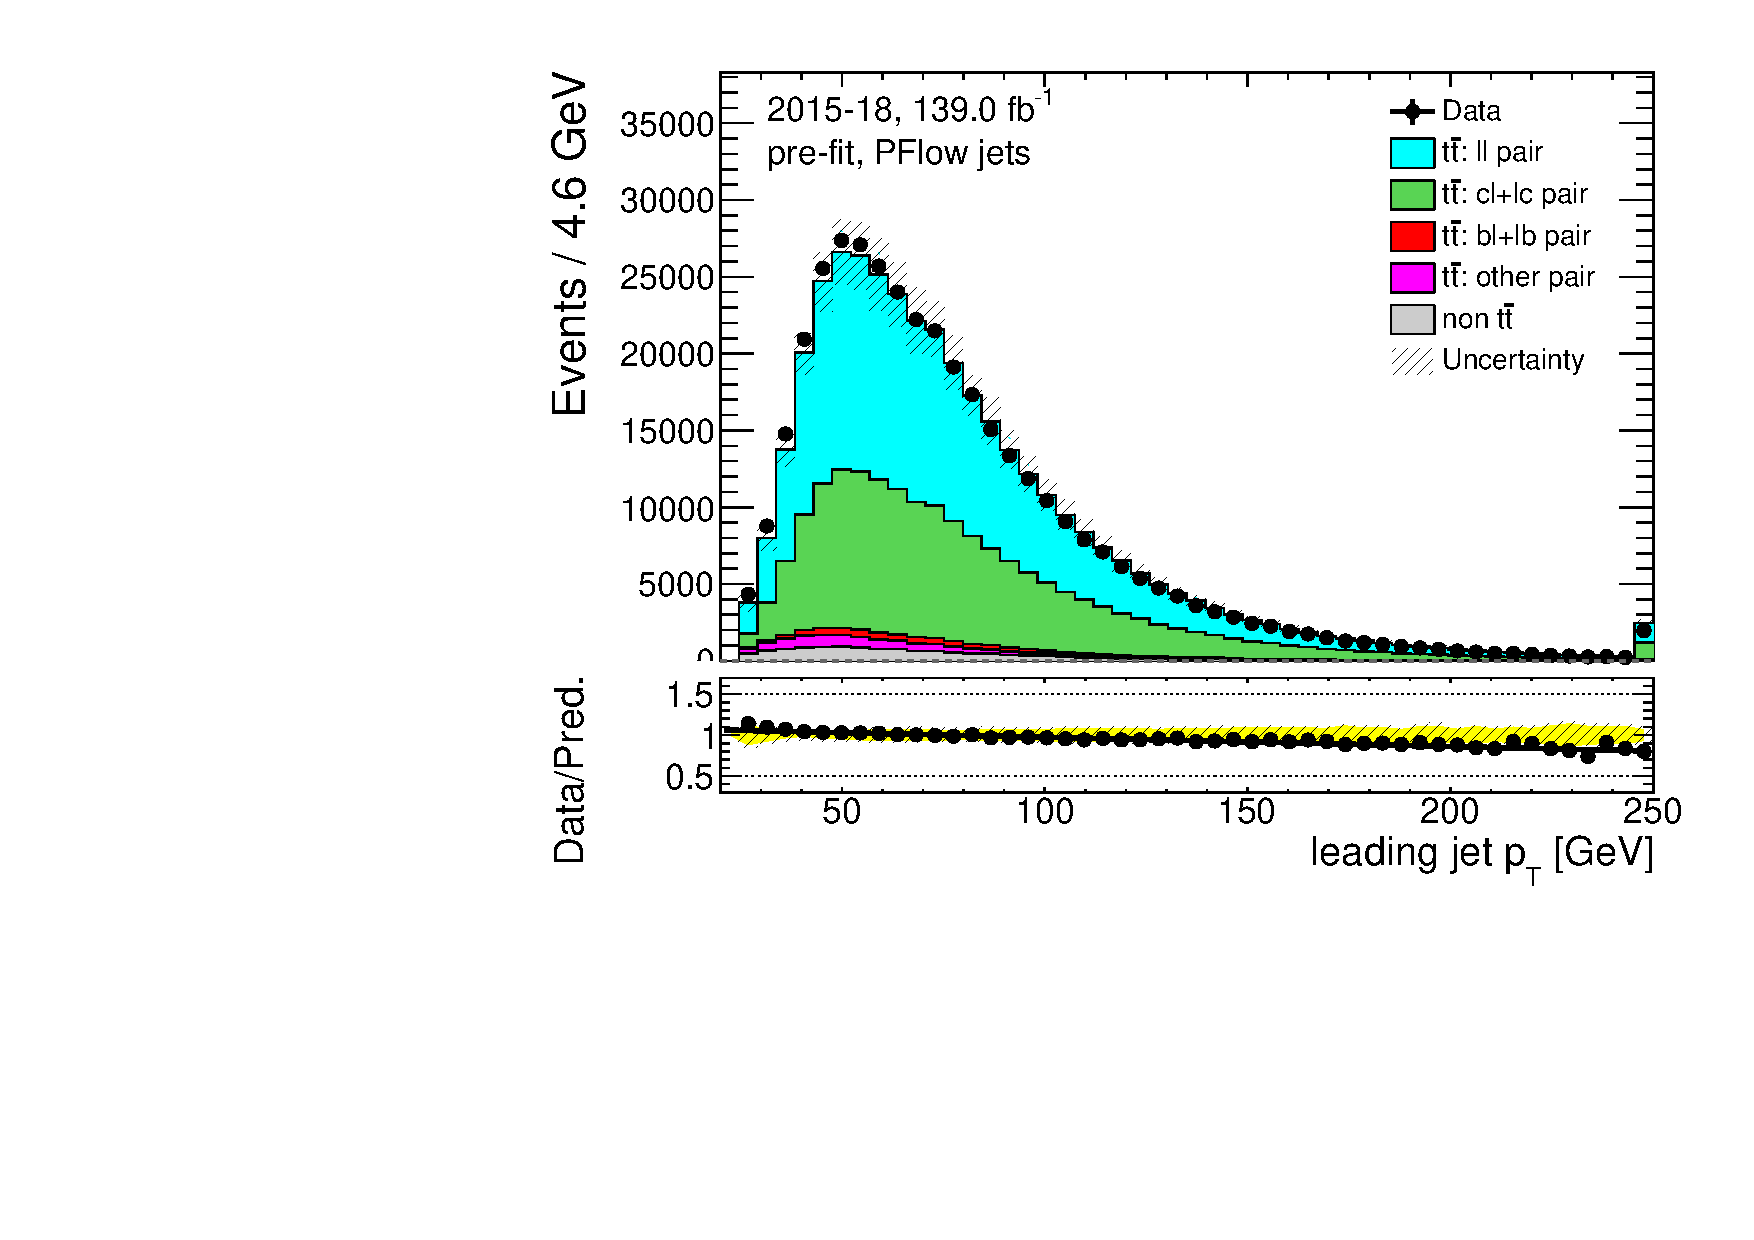
\includegraphics[width=0.45\textwidth]{FTAG_plots/pretagNoRwwithhighpTPFlowall/DataMC_h_J0_pt.pdf}
		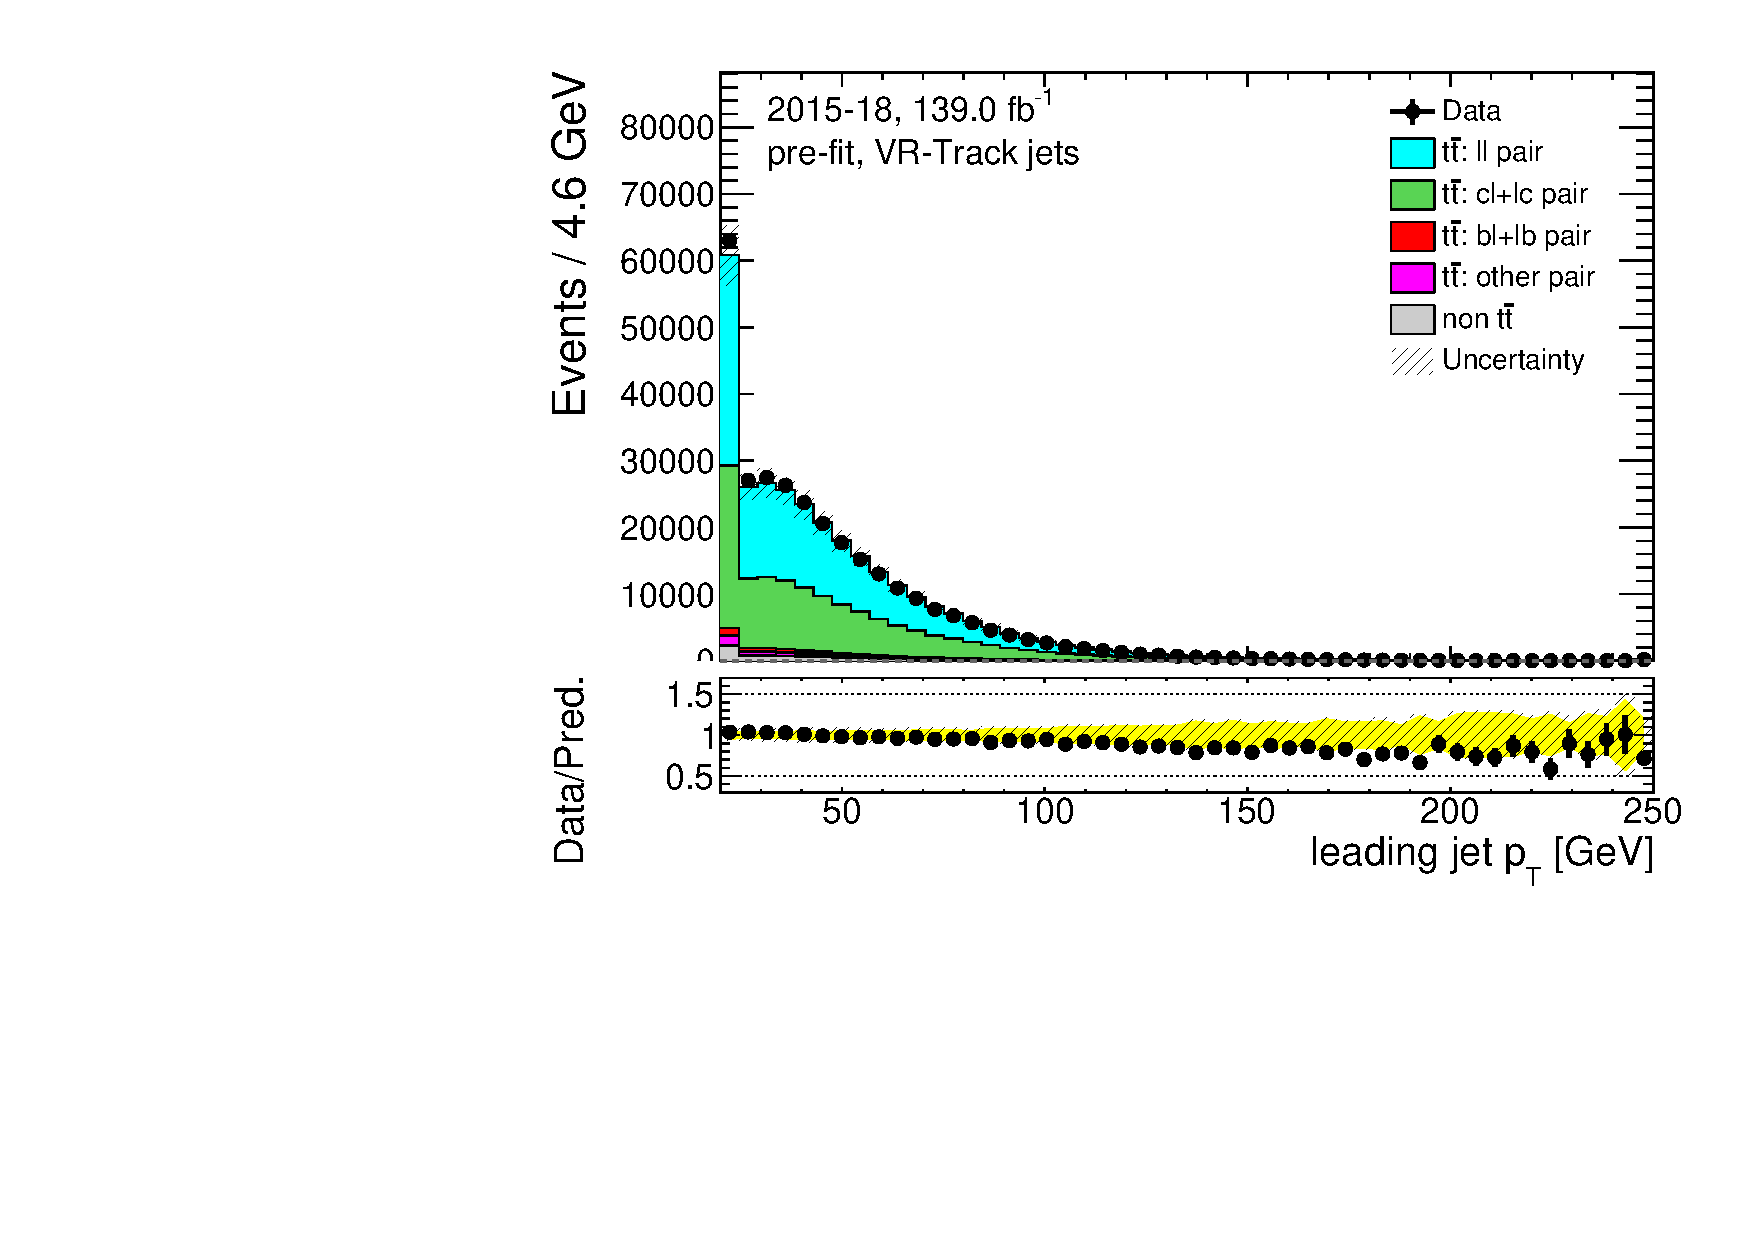
\includegraphics[width=0.45\textwidth]{FTAG_plots/pretagNoRwwithhighpTVRJetsall/DataMC_h_J0_pttrackjet.pdf}\\
		\includegraphics[width=0.45\textwidth]{FTAG_plots/pretagNoRwwithhighpTPFlowall/DataMC_h_J1_pt.pdf}
		\includegraphics[width=0.45\textwidth]{FTAG_plots/pretagNoRwwithhighpTVRJetsall/DataMC_h_J1_pttrackjet.pdf}\\
		\caption{Combined selection: data versus simulation of $W$ jets\pt\ for 
		PFlow jets in the left column and for VR-Track jets in the right column.}
		\label{fig:kinematic_distributions_combined}
\end{figure}
		

\section{Systematic uncertainties}
\label{sec:FTAG_systematics}
The systematic uncertainties considered and propagated in this calibration 
can be broadly categorised into experimental and modelling systematic uncertainties. 
\subsection{Experimental uncertainties}
TODO: refer to the analysis Part
Experimental uncertainties are related to the detector and estimated using 
data-driven methods or MC simulations. 
The lepton energy scale and resolution are corrected to 
provide better agreement between MC predictions and data, uncertainties 
due the corrections are considered. Uncertainties are taken into account on the 
electron and muon trigger, identification and reconstruction efficiencies, and for 
uncertainties associated with the isolation requirements. 

The jet energy scale (JES) uncertainty depends on $p_T$ and $\eta$ and 
takes into account uncertainties due to pile-up effects. Uncertainties on the jet energy resolution (JER) 
are taken into account. Uncertainties on the energy scale and resolution of 
the electrons, muons, jets and taus are propagated to the calculation of the \MET, 
which also has additional dedicated uncertainties on the scale, resolution, and 
reconstruction efficiency of tracks not associated to any of the reconstructed objects,
 along with the modelling of the underlying event. Uncertainties on the $b$-tagging (mis-tagging) 
 probabilities for $b$ (light) jets are considered both for the tagging jets assigned to the $b$ quark 
 from the top decay and for the jets associated to the hadronically decaying $W$ boson.
Supporting material for this section can be found in the appendix, Tab.\ref{tab:systematics}.
%The uncertainty on these corrections is taken into account as a shape-dependent systematic uncertainty in the final fit of the backgrounds and signal models.

\subsection{Modelling uncertainties} 
The uncertaity due to different choices of the parton shower models is estimated by comparing
the MC samples generated with nominal parton shower model and with the 
alternative parton shower model.
More specifically, it is derived 
by comparing the prediction from \powheg interfaced either to \pythia or \Herwigpp. 
The uncertainty due to additional radiation in 
the initial state and the final state is estimated by comparing the nominal MC samples with the MC samples 
with alternative scale of renormalisation and factorisation.
The uncertainty on modelling of initial state radiation (ISR) is assessed with two alternative \powhegpythia 
samples. The samples include one with an increase in radiation which has the renormalisation and 
factorisation scales decreased by a factor of two and the \textit{hdamp} parameter doubled 
(which controls the \pt\ of the first additional emission), while 
the sample with a decrease in radiation has the scales increased by a factor of two. 
In all cases, MC-to-MC SFs are taken into account.
In addition, the uncertainty due to the
variations samples being produced by fast simulation while the nominal samples being 
produced full simulation is also considered.
The comparisons of 
the nominal \ttbar\ sample and the samples with each systematic uncertainty 
are shown in Table \ref{tab:modelling_syst}. 



\begin{table}[ht]
	\centering
	\small
	\setlength\tabcolsep{5pt} 
	\newcolumntype{C}{ @{}>{${}}c<{{}$}@{} }
	\begin{tabular}{|r *2{|rCr|r}| }
	\hline
	& \multicolumn{4}{|c|}{PFlow jets} & \multicolumn{4}{c|}{Track jets} \\
	\hline
	& \multicolumn{3}{c|}{Yields} & \specialcell{Ratio of \\difference to \\nominal sample} & \multicolumn{3}{c|}{Yields} & \specialcell{Ratio of \\difference to\\ nominal sample} \\
	\hline
	\ttbar\ Nominal &	 385378  &\pm&  230 &         &   	  302690 &\pm&  200   &  \\
	Data/MC         &        0.973  &\pm&  0.002 &      &     0.971 &\pm&  0.002 &         \\
	\hline
	\ttbar\ AF2     &    386260  &\pm&  250  &  0.716\% &     304860  &\pm&  230  &  0.716\%\\
	DATA/MC(AF2)    &    0.967  &\pm&  0.002  &          &    0.965  &\pm&  0.002   &      \\              
	\hline
	\ttbar\ ISR     &    377130  &\pm&  220  & -1.665\% &     297960  &\pm&  200  & -1.562\%\\     
	DATA/MC(ISR)    &    0.989  &\pm&  0.002  &          &    0.986  &\pm&  0.002   &  \\       
	\hline
	\ttbar\ \Herwig &    331960  &\pm&  220  & -13.443\%&     259940  &\pm&  190  & -14.123\%\\ 
	DATA/MC(\Herwig)&    1.119  &\pm&  0.002  &          &    1.126  &\pm&  0.002   &\\                
	\hline
	\end{tabular}
	\vspace{0.2cm}
	\caption{Comparison of the number of events in data and in 
	simulation considering the PFlow jets and the VR-Track jets for an inclusive
	selection. The uncertainty due to the variations samples being produced 
	by fast simulation is included in the table as \ttbar\ AF2. }
	\label{tab:modelling_syst}
	\end{table}


\section{Under-estimation of $t\bar{t}$ + Heavy flavour background }
Depsite the fact that the true nature of most of the reconstructed $W$ jets are either 
\cjets\ or light jets, there is still a very small amount of them are true \bjets. 

There are two main sources of these true \bjets. The first is a $W$ boson 
decays to a $b$ and a $c$ quark. The second is 
when the $t\bar{t}$ plus a gluon process (referred to as \ttbar\ + heavy flavour process)
is selected, and the gluon splits
into a pair a $b$ quarks and one of them is assigned as a $W$ jet. 
The first source can be excluded by requiring no \cjets in the $W$ jets,
meaning the true \bjet\ in the $W$ jets 
can only come from the $t\bar{t}$ + heavy flavour 
process. This process is underestimated by the MC by about 30\% 
for both the PFlow and VR-Track jets collections, as shown in Table \ref{tab:3byields1} 
and Figure~\ref{fig:3bplots}, where an extra cut requiring at least one $W$ jet with DL1r $> 8$ 
is added to the combined selection to reject most of the true \cjets and true light jet. 
A more thorough study is done in Ref.~\cite{TOPQ-2017-12}, where the mis-modelling 
factor is measured to be $1.25 \pm 0.25$, which is also consistent with the $30\%$ 
mismodelling observed in the previous study. 
Therefore, events in the simulation
in which the top jets and at least one of the $W$ jets are \bjets (referred to as 3 true \bjets\ events), 
are scaled by $1.25 \pm 0.25$.
All results shown in this chapter have this scale factor implemented, 
and the full difference between the simulation before applying this scale factor and 
after is taken as a systematic uncertainty. This uncertainty has been added in quadrature 
to the systematic uncertainties described in Section \ref{sec:FTAG_systematics} 
in all the plots in this chapter.



\begin{table}[ht]
    \centering
	\newcolumntype{C}{ @{}>{${}}c<{{}$}@{} }
	\begin{tabular}{|r *2{|rCr}| }
		\hline
		& \multicolumn{3}{|c|}{PFlow jets} & \multicolumn{3}{c|}{VR-Track jets} \\
		\hline
        Data & 1589& & & 1336  & & \\
         $t\bar{t}$ & 1100  &\pm&  13	& 940  &\pm&  12\\
         Non \ttbar\ 		& 83  &\pm&  6		& 69  &\pm&  5  \\
		 Data/MC 	& 1.34  &\pm&  0.04 & 1.32  &\pm&  0.04 \\
		 \hline
    \end{tabular}
	\caption{Yields of the 2018 data and MC of the combined selection, 
	requiring at least 1 PFlow or track $W$ jet with DL1r > 8 to 
	reject most of the light- and \cjets.}
    \label{tab:3byields1}
\end{table}


\begin{figure}[bth]
    \centering
\includegraphics[width=.45\textwidth]{FTAG_plots/3bplots/3bplots.png}
	\caption{The DL1r score distribution of the leading VR-Track jet, 
	requiring at least 1 VR-Track jets have DL1r > 8 to reject most of 
	the light and the $c$ jets, with $t\bar{t}$ modelling and statistical uncertainties. }
    \label{fig:3bplots}
\end{figure}


\section{Results}
\label{result}


\subsection{Overview}
Four rounds of calibrations have been carried out, containing different 
jet collections, Monte Carlo samples, analysis framework 
and \bjet\ identification algorithm. 
In the latest round, 
the calibration includes the PFlow jet and the VR-Track jet collection, 
and MV2c10, DL1 and DL1r taggers. The low-$p_T$ 
selection and the standard selection are carried out for all four 
calibrations, while the high-$p_T$ selection is only implemented 
in the latest calibration. 

\subsection{\btagging\ algorithms output distribution}
The distributions of the \btagging\ algorithm' output of 
the MC and the data of the latest calibration 
(December 2020) are shown in Figure~\ref{fig:taggers_PFlow} for the PFlow jets and 
Figure~\ref{fig:taggers_VRJets} for the VR-Track jets, 
combining the standard selection, low \pt\ and the high-$p_T$ selection. 
In these figure, the data events are compared against the simulation.
The majority of the events come from \ttbar\ production. There is only
a very small fraction of non \ttbar\ events. The $W$ jets pairs are mostly light jets 
pairs and \cjet\ light jet pairs, and a very small fraction of the pairs are 
\bjet\ light jet pairs or pairs containing one or more $\tau$ hadron(s). 
The yellow band in the lower pad indicates the overall systematic uncertainties
and the black band represents the \ttbar\ modelling systematic uncertainty, 
which dominates at low \btagging\ discriminant (DL1 or DL1r < 4). 
The experimental systematic uncertainty is in general very small. 
At high \btagging\ discriminant (DL1 or DL1r > 4), the
uncertainty due to the $1.25 \pm 0.25$ scale factor 
becomes more important. 
\begin{figure}[H]
	\begin{subfigure}[t]{1\linewidth}
	\includegraphics[width=.45\textwidth]{FTAG_plots/pretagNoRwwithhighpTPFlowall/DataMC_h_J0_DL1_log.png}
	\includegraphics[width=.45\textwidth]{FTAG_plots/pretagNoRwwithhighpTPFlowall/DataMC_h_J1_DL1_log.png}\\
	\caption{DL1 tagger output}
	\end{subfigure}
	\begin{subfigure}[t]{1\linewidth}
		\includegraphics[width=.45\textwidth]{FTAG_plots/pretagNoRwwithhighpTPFlowall/DataMC_h_J0_DL1r_log.png}
		\includegraphics[width=.45\textwidth]{FTAG_plots/pretagNoRwwithhighpTPFlowall/DataMC_h_J1_DL1r_log.png}\\
		\caption{DL1r tagger output}
	\end{subfigure}
	\begin{subfigure}[t]{1\linewidth}
	\includegraphics[width=.45\textwidth]{FTAG_plots/pretagNoRwwithhighpTPFlowall/DataMC_h_J0_MV2c10_log.png}
	\includegraphics[width=.45\textwidth]{FTAG_plots/pretagNoRwwithhighpTPFlowall/DataMC_h_J1_MV2c10_log.png}\\
	\caption{MV2c10 tagger output}
	\end{subfigure}
	\caption{PFlow jets: distributions of the DL1, DL1r and MV2c10 
	tagger outputs of the combined selection, 
	leading jet in the left column and sub-leading jet in the right column,
	before fitting or tagging with full uncertainties.} \label{fig:taggers_PFlow}
\end{figure}
\newpage
\begin{figure}[H]
	\begin{subfigure}[t]{1\linewidth}
	\includegraphics[width=.45\textwidth]{FTAG_plots/pretagNoRwwithhighpTVRJetsall/DataMC_h_J0_DL1trackjet_log.png}
	\includegraphics[width=.45\textwidth]{FTAG_plots/pretagNoRwwithhighpTVRJetsall/DataMC_h_J1_DL1trackjet_log.png}\\
	\caption{DL1 tagger output}
	\end{subfigure}
	\begin{subfigure}[t]{1\linewidth}
	\includegraphics[width=.45\textwidth]{FTAG_plots/pretagNoRwwithhighpTVRJetsall/DataMC_h_J0_DL1rtrackjet_log.png}
	\includegraphics[width=.45\textwidth]{FTAG_plots/pretagNoRwwithhighpTVRJetsall/DataMC_h_J1_DL1rtrackjet_log.png}\\
	\caption{DL1r tagger output}
	\end{subfigure}
	\begin{subfigure}[t]{1\linewidth}
	\includegraphics[width=.45\textwidth]{FTAG_plots/pretagNoRwwithhighpTVRJetsall/DataMC_h_J0_MV2c10_Fulltrackjet_log.png}
	\includegraphics[width=.45\textwidth]{FTAG_plots/pretagNoRwwithhighpTVRJetsall/DataMC_h_J1_MV2c10_Fulltrackjet_log.png}\\
	\caption{MV2c10 tagger output}
	\end{subfigure}
	\caption{VR-Track jets: distributions of the DL1, DL1r and MV2c10 tagger outputs of 
	the combined selection, 
	leading jet in the left column and sub-leading jet in the right column,
	before fitting or tagging with full uncertainties.} \label{fig:taggers_VRJets}
\end{figure}	

\subsection{Efficiencies and Scale Factors}
%The Monte Carlo simulation demonstrates good agreement in different kinematic variables with data. 
The Dl1 and DL1r \cjet efficiencies and scale factors with systematics 
uncertainties are calculated with four fixed cut working points 
for the PFlow and VR VR-Track jets collection in the latest derivation 
in December 2020.

The \cjet\ mis-tagging efficiencies are shown in Figure~\ref{fig:Dec_eff_PFlow_DL1}-\ref{fig:Dec_eff_VRJets_DL1r} 
for the PFlow jet collections and the VR-Track jets with the DL1 and the DL1r tagger. 
For PFlow jets, these results combine the standard selection, low\pt\ selection and the high-$p_T$ selection 
and for the VR-Track jets they combine the standard selection and the high-$p_T$ selection. 

The $1.25 \pm 0.25$ scale factor is applied on events with 3 true \bjets. 
The overall uncertainties are shown 
in the red band. 
The scale factors are shown in Figure~\ref{fig:Dec_SF_PFlow_DL1}-\ref{fig:Dec_SF_VRJets_DL1r} for the PFlow jets
and the VR-Track jets with the DL1 and DL1r tagger. 
The tighter working points (60\%, 70\%) show larger uncertainties and bigger deviation from 1, while
the looser working points (77\%, 85\%) have much smaller uncertainty and the simulation is able to 
recover the data well due to more abundant events statistics.
For the PFlow jets, in most of the working points the systematic uncertainties dominate 
in the low-\pt\ bins (\pt\ < 150) and the statistical error, represented by the error bars on the 
markers, become more important in the last bin. 
For the VR-Track jets the statistical uncertainty is relatively constant for all bins while the 
systematic uncertainty increases as the \pt\ increases. 
To demonstrate the effect on statistics with the high-\pt\ selection, 
the fractional statistical uncertainties of 60\% working point scale factor
are shown in Table \ref{tab:stats_gain} for the standard and the combined selection.
In some bins the statistical uncertainty can decrease up to 30\%, suggesting that the
high-\pt\ selection is successful at increasing events statistics. 

\begin{table}[ht]
	\centering
	\small
	\setlength\tabcolsep{5pt} 
	\begin{tabular}{|r *2{|rr|r}| }
	\hline
	& \multicolumn{3}{|c|}{PFlow jets} & \multicolumn{3}{c|}{VR-Track jets} \\
	\hline
	&  \specialcell{Standard\\ selection} &\specialcell{ High-\pt\ \\selection }&\specialcell{ Fractional \\decrease} &  \specialcell{Standard\\ selection} &\specialcell{ High-\pt\ \\selection }&\specialcell{ Fractional \\decrease}\\
	\hline
	Bin No.1    &	 3.3\%  &3.3\% & 0.0\% & 5.6\%  & 5.3\%      &  5.7\%  \\
	Bin No.2    &    3.1\%  &2.8\% & 10.7\% & 4.2\%  & 3.7\%     & 13.5\%   \\
	Bin No.3    &    3.4\%  &2.6\% & 30.8\% & 5.8\%  & 4.9\%     & 18.4\%   \\
	Bin No.4    &    12.1\% &9.3\% & 30.1\% & 7.2\%  & 5.6\%     & 28.6\%   \\           
	\hline                 
	\end{tabular}
	\vspace{0.2cm}
	\caption{Comparison of the fractional statistical uncertainty in the DL1r 60\%
	working point scale factor. The \pt\ range of each bin can be found in section \ref{sec:Calibration method for charm jet}. }
	\label{tab:stats_gain}
	\end{table}



\newpage
%%% Efficiencies plots %%%

\begin{figure}[H]
	\centering
	\begin{subfigure}[t]{.35\linewidth}
\includegraphics[width=1\textwidth]{FTAG_plots/DL1allPFlowDec/eff60.eps}
\caption{60\% working point}
	\end{subfigure}
\begin{subfigure}[t]{.35\linewidth}
	\includegraphics[width=1\textwidth]{FTAG_plots/DL1allPFlowDec/eff70.eps}
	\caption{70\% working point}
\end{subfigure}
\begin{subfigure}[t]{.35\linewidth}
\includegraphics[width=1\textwidth]{FTAG_plots/DL1allPFlowDec/eff77.eps}
\caption{77\% working point}
\end{subfigure}
\begin{subfigure}[t]{.35\linewidth}
\includegraphics[width=1\textwidth]{FTAG_plots/DL1allPFlowDec/eff85.eps}
\caption{85\% working point}
\end{subfigure}
\caption{Charm-jet efficiencies for the PFlow jets collection with
the DL1 tagger.} \label{fig:Dec_eff_PFlow_DL1}
\end{figure}

\begin{figure}[H]
	\centering
	\begin{subfigure}[t]{.35\linewidth}
		\includegraphics[width=1\textwidth]{FTAG_plots/DL1rallPFlowDec/eff60.eps}
		\caption{60\% working point}
			\end{subfigure}
		\begin{subfigure}[t]{.35\linewidth}
			\includegraphics[width=1\textwidth]{FTAG_plots/DL1rallPFlowDec/eff70.eps}
			\caption{70\% working point}
		\end{subfigure}
		\begin{subfigure}[t]{.35\linewidth}
		\includegraphics[width=1\textwidth]{FTAG_plots/DL1rallPFlowDec/eff77.eps}
		\caption{77\% working point}
		\end{subfigure}
		\begin{subfigure}[t]{.35\linewidth}
		\includegraphics[width=1\textwidth]{FTAG_plots/DL1rallPFlowDec/eff85.eps}
		\caption{85\% working point}
		\end{subfigure}
		\caption{Charm-jet efficiencies for the PFlow jets collection with
	the DL1r tagger.} \label{fig:Dec_eff_PFlow_DL1r}
\end{figure}


\newpage
\begin{figure}[H]
	\centering
	\begin{subfigure}[t]{.35\linewidth}
		\includegraphics[width=1\textwidth]{FTAG_plots/DL1allVRJetsDec/eff60.eps}
		\caption{60\% working point}
			\end{subfigure}
		\begin{subfigure}[t]{.35\linewidth}
			\includegraphics[width=1\textwidth]{FTAG_plots/DL1allVRJetsDec/eff70.eps}
			\caption{70\% working point}
		\end{subfigure}
		\begin{subfigure}[t]{.35\linewidth}
		\includegraphics[width=1\textwidth]{FTAG_plots/DL1allVRJetsDec/eff77.eps}
		\caption{77\% working point}
		\end{subfigure}
		\begin{subfigure}[t]{.35\linewidth}
		\includegraphics[width=1\textwidth]{FTAG_plots/DL1allVRJetsDec/eff85.eps}
		\caption{85\% working point}
		\end{subfigure}
	\caption{Charm-jet efficiencies for the VR-Track jets collection with
	the DL1 tagger.} \label{fig:Dec_eff_VRJets_DL1}
	\end{figure}

	\begin{figure}[H]
		\centering
		\begin{subfigure}[t]{.35\linewidth}
			\includegraphics[width=1\textwidth]{FTAG_plots/DL1rallVRJetsDec/eff60.eps}
			\caption{60\% working point}
				\end{subfigure}
			\begin{subfigure}[t]{.35\linewidth}
				\includegraphics[width=1\textwidth]{FTAG_plots/DL1rallVRJetsDec/eff70.eps}
				\caption{70\% working point}
			\end{subfigure}
			\begin{subfigure}[t]{.35\linewidth}
			\includegraphics[width=1\textwidth]{FTAG_plots/DL1rallVRJetsDec/eff77.eps}
			\caption{77\% working point}
			\end{subfigure}
			\begin{subfigure}[t]{.35\linewidth}
			\includegraphics[width=1\textwidth]{FTAG_plots/DL1rallVRJetsDec/eff85.eps}
			\caption{85\% working point}
			\end{subfigure}
		\caption{Charm-jet efficiencies for the VR-Track jets collection with
		the DL1r tagger.} \label{fig:Dec_eff_VRJets_DL1r}
\end{figure}

\newpage
%SF plots
\begin{figure}[H]
	\centering
	\begin{subfigure}[t]{.35\linewidth}
		\includegraphics[width=1\textwidth]{FTAG_plots/DL1allPFlowDec/SF60.eps}
		\caption{60\% working point}
			\end{subfigure}
		\begin{subfigure}[t]{.35\linewidth}
			\includegraphics[width=1\textwidth]{FTAG_plots/DL1allPFlowDec/SF70.eps}
			\caption{70\% working point}
		\end{subfigure}
		\begin{subfigure}[t]{.35\linewidth}
		\includegraphics[width=1\textwidth]{FTAG_plots/DL1allPFlowDec/SF77.eps}
		\caption{77\% working point}
		\end{subfigure}
		\begin{subfigure}[t]{.35\linewidth}
		\includegraphics[width=1\textwidth]{FTAG_plots/DL1allPFlowDec/SF85.eps}
		\caption{85\% working point}
		\end{subfigure}
	\caption{Charm-jet scale factors for the PFlow jets collection with 
	the DL1 tagger.} \label{fig:Dec_SF_PFlow_DL1}
	\end{figure}
	

\begin{figure}[H]
	\centering
	\begin{subfigure}[t]{.35\linewidth}
		\includegraphics[width=1\textwidth]{FTAG_plots/DL1rallPFlowDec/SF60.eps}
		\caption{60\% working point}
			\end{subfigure}
		\begin{subfigure}[t]{.35\linewidth}
			\includegraphics[width=1\textwidth]{FTAG_plots/DL1rallPFlowDec/SF70.eps}
			\caption{70\% working point}
		\end{subfigure}
		\begin{subfigure}[t]{.35\linewidth}
		\includegraphics[width=1\textwidth]{FTAG_plots/DL1rallPFlowDec/SF77.eps}
		\caption{77\% working point}
		\end{subfigure}
		\begin{subfigure}[t]{.35\linewidth}
		\includegraphics[width=1\textwidth]{FTAG_plots/DL1rallPFlowDec/SF85.eps}
		\caption{85\% working point}
		\end{subfigure}
	\caption{Charm-jet scale factors for the PFlow jets collection with 
	the DL1r tagger.} \label{fig:Dec_SF_PFlow_DL1r}
	\end{figure}	
\newpage
\begin{figure}[H]
	\centering
	\begin{subfigure}[t]{.35\linewidth}
		\includegraphics[width=1\textwidth]{FTAG_plots/DL1allVRJetsDec/SF60.eps}
		\caption{60\% working point}
			\end{subfigure}
		\begin{subfigure}[t]{.35\linewidth}
			\includegraphics[width=1\textwidth]{FTAG_plots/DL1allVRJetsDec/SF70.eps}
			\caption{70\% working point}
		\end{subfigure}
		\begin{subfigure}[t]{.35\linewidth}
		\includegraphics[width=1\textwidth]{FTAG_plots/DL1allVRJetsDec/SF77.eps}
		\caption{77\% working point}
		\end{subfigure}
		\begin{subfigure}[t]{.35\linewidth}
		\includegraphics[width=1\textwidth]{FTAG_plots/DL1allVRJetsDec/SF85.eps}
		\caption{85\% working point}
		\end{subfigure}
	\caption{Charm-jet scale factors for the VR-Track jets collection with 
	the DL1 tagger.} \label{fig:Dec_SF_VRJets_DL1}
	\end{figure}
	

\begin{figure}[H]
	\centering
	\begin{subfigure}[t]{.35\linewidth}
		\includegraphics[width=1\textwidth]{FTAG_plots/DL1rallVRJetsDec/SF60.eps}
		\caption{60\% working point}
			\end{subfigure}
		\begin{subfigure}[t]{.35\linewidth}
			\includegraphics[width=1\textwidth]{FTAG_plots/DL1rallVRJetsDec/SF70.eps}
			\caption{70\% working point}
		\end{subfigure}
		\begin{subfigure}[t]{.35\linewidth}
		\includegraphics[width=1\textwidth]{FTAG_plots/DL1rallVRJetsDec/SF77.eps}
		\caption{77\% working point}
		\end{subfigure}
		\begin{subfigure}[t]{.35\linewidth}
		\includegraphics[width=1\textwidth]{FTAG_plots/DL1rallVRJetsDec/SF85.eps}
		\caption{85\% working point}
		\end{subfigure}
	\caption{Charm-jet scale factors for the VR-Track jets collection with 
	the DL1r tagger.} \label{fig:Dec_SF_VRJets_DL1r}
	\end{figure}	


\newpage
\iffalse


In terms of statistical gain, taking the 60\% working point scale factor with 2018 data as an example, the error is reduced as expected. In the last bin of the $p_{T}$ distribution of scale factors, the error is reduced by 55\%, which suggests the success of high-$p_{T}$ selection method. The percentage reduction of error of each bin is given in Tab.\ref{tab:limit}:


 \begin{table}[ht]
 \begin{centering}
 \begin{tabular}{|p{2.5em}||p{2.5em}|p{2.5em}|p{5em}||p{2.5em}|p{2.5em}|p{5em}||p{5em}|}
          \hline
          & \multicolumn{3}{|c||}{high-$p_{T}$ + standard selection} & \multicolumn{3}{|c||}{standard selection only} & \\  \hline\hline
          Bins& Bin Value &Bin error&Percentage error&Bin Value &Bin error&Percentage error & Error reduction\\ \hline
          Bin 1 & 1.25 & 0.12 & 10\% &1.20 & 0.13 & 11\% & 11\% \\ \hline
          Bin 2 & 1.34 & 0.10 & 8\% & 1.24 & 0.11 & 9\% & 18\% \\ \hline
          Bin 3 & 1.22 & 0.10 & 8\% & 1.04 & 0.11 & 10\% & 28\% \\ \hline
          Bin 4 & 0.98 & 0.24 & 24\% & 0.72 & 0.27 & 37\% & 55\% \\ \hline
          
 
 \end{tabular} 
 \caption{Bins values and the corresponding errors of the scale factor at 60\% working point, with 2018 data.}
 \end{centering}
 \label{tab:limit}
 \end{table}

\fi

\newpage




\large
\chapter{Search for Higgs boson pair production in the \bbttlh channel}
\label{sec:search for dihiggs}
due: 15/12
This chapter describes the search for Higgs boson pair production in the
\bbtt\ channel, where one Higgs boson decays to a \bquark\ pair 
and the other to a $\tau$-lepton pair. 
As the two $\tau$-leptons decay either leptonically or hadronically, 
the analysis is divided further into two sub-channels depending on
their decay mode, 
the $b\bar{b}\tau_{\text{lep}}^{\pm}\tau_{\text{had}}^{\mp}$ channel 
(for simplicity, referred to as \lephad channel)
where one of the $\tau$-leptons decays leptonically and the other decays
hadronically, 
and the \bbtthh\ channel (or referred to as \hadhad channel) 
where both of the $\tau$-leptons decay hadronically. 
The decay mode of both $\tau$-leptons decay
leptonically is not considered in this analysis 
due to its insignificant contribution. 
In this thesis, the author will present his work 
in the \lephad channel, and will also show the combination results with 
the \hadhad channel.


% one of the $\tau$-leptons decay leptonically and the other decay hadronically. 
The results of this search are interpreted in terms of resonant and 
non-resonant production of the di-Higgs.
For the non-resonant production, upper limits are set on the SM di-Higgs production
cross section, and exclusion limits are set on the Higgs self-coupling $\lambda_{HHH}$.
% The non-resonant search is also interpreted in terms of the coupling modifiers using a
% Higgs Effective Field Theory approach .
For the resonant search, upper limits are set on the resonance production cross section 
as a function of the resonance mass, targeting a generic spin-0 neutral scalar. 
The \lephad and \hadhad
combination results are published in Ref.\cite{dihiggs-conf}.
The $\lambda_{HHH}$ result is combined with other final states of the di-Higgs production
including \bbbb\ and \bbyy. 
The combination result is published in Ref.~\cite{ATLAS-CONF-2021-052}. 

The analysis strategy is as follows:
first, a set of selections are applied on 
the reconstructed physics objects and kinematics variables which
defines the signal regions and the control region, 
as decribed in section~\ref{sec:DiHiggs:selection};
neural networks trained on the signal regions events are then 
used to extract the various signals, and the output of the algorithm is used
as the final discriminant, as described in section~\ref{sec:DiHiggs:MVA};
the systematic uncertainties considered in this analysis is discussed in 
section~\ref{sec:DiHiggs:systematics};
a profile likelihood fit is then performed simultaneously on all \lephad and \hadhad
signal regions and the control region, with all systematics uncertainties served as nuisance parameters.
The statistical combination result of \bbtt, \bbyy and \bbbb is also studied. 
The setup and the results are shown in section~\ref{sec:DiHiggs:results}.

The author's contributions to the analyses presented in this Chapter are as follows.
As one of the main analysers in the \lephad channel, 
the author produced all data and MC (including all signals and background) 
histograms with full experimental and theoretical systematics, which are the inputs to the likelihood fit. 
The author has derived the systematics uncertainties for the following major backgrounds:
\ttbar, \ZHF\ and single-top. The author has also contributed to the estimation of the fake-\tauhad\
background and its uncertainties. 
Finally, the author implemented and validated a reweighting method in order to scan
the non-resonant $HH$ production with in various \kl\ values, and derived the corresponding
uncertainties. 
% 

\section{Data and Monte Carlo Simulation}
\subsection{Data}
The results presented here are based on proton–proton collision data 
at a centre-of-mass energy of \sqrts = 13 TeV, 
collected by the ATLAS detector at the LHC between 2015 and 2018, 
corresponding to an integrated luminosity of \lumi. 
Selected data events are required to have all relevant components 
of the ATLAS detector in good working condition 
according to the ATLAS Good-Run-List (GRL). 
In the following, a description of the signal and 
background Monte Carlo samples is given. 
Supporting material for this section can be found in appendix B, 
including the data GRL and the complete signal and background Monte Carlo samples list.
 
 \subsection{Signal Monte Carlo Samples}


 The SM non-resonant di-Higgs process via gluon-gluon fusion 
 was simulated with \POWHEGBOX v2 generator~\cite{Powheg1, Powheg2, Powheg3} 
 at next-to-leading order (NLO), with full NLO corrections with finite top mass, 
 using the PDF4LHC~\cite{Butterworth:2015oua} parton distribution function (PDF) set. 
 Parton showers and hadronization were simulated with \PYTHIA8 version 8.244~\cite{PYTHIA82} 
 parton shower model, with the A14 set of tuned parameters~\cite{A14tune, ATLAS:2012uec} 
 and the NNPDF23LO PDF set~\cite{NNPDF23PDFSet}. 
 The EvtGen v1.6.0 program~\cite{EvtGen} is used to model 
 the properties of the bottom and charm hadron decays.

 The normalisation of this process in the analysis is set to the SM ggF di-Higgs cross section, $\sigma_{ggF}=\SI{31.05}{fb}$ calculated at NNLO FTApprox~\cite{Grazzini:2018bsd}, times the $bb\tau\tau$ BR, $\sigma_{ggF} \times BR (bb \tau\tau)  = \SI{31.05}{fb} \times 0.0730562561  =  \SI{2.2683967}{fb}$.  
 
 The SM non-resonant di-Higgs process via vector boson fusion (VBF) was generated at leading-order (LO) using \MADGRAPH version 2.7.3~\cite{mg5_lo}, with the NNPDF30NLO~\cite{NNPDF} PDF set. Parton showering and hadronization are performed using \PYTHIA8 version 8.244~\cite{PYTHIA82} with the A14 set of tuned parameters~\cite{A14tune, ATLAS:2012uec} and the NNPDF23LO PDF set~\cite{NNPDF23PDFSet}. The EvtGen  v1.7.0 program~\cite{EvtGen} is used for the bottom and charm hadron decays.
 
 This process is normalised to the SM VBF HH cross section, $\sigma_{VBF}=\SI{1.726}{fb}$ calculated at N3LO QCD~\cite{Dreyer_2018}, times the $bb\tau\tau$ BR, $\sigma_{VBF} \times BR (bb \tau\tau)  = \SI{1.726}{fb} \times 0.0730562561  =  \SI{0.126095098}{fb}$.  
 
 The resonant di-Higgs production process via gluon-gluon fusion, $pp \rightarrow X \rightarrow HH$, was
 simulated in the extended Higgs sector of Two-Higgs-Doublet Models
 (2HDM)~\cite{Branco:2011iw} in the narrow width approximation. Simulated
 resonant di-Higgs samples were produced for 18 mass points (251, 260, 280, 300, 325, 350, 400, 450, 500, 550, 600, 700, 800,
 900, 1000, 1200, 1400, 1600 \GeV), with the Standard Model Higgs boson ($H$) mass set to $m_H=125$
 \GeV. The narrow width scalar model is a gluon-initiated state (ggF) implemented in
 \MADGRAPH at leading-order (LO)~\cite{mg5_lo} and interfaced to the \Herwig7 version 7.1.0.3~\cite{Herwigpp}
 parton shower model. The EvtGen v1.6.0 program~\cite{EvtGen} is used to model the properties of the bottom and charm hadron decays. 
 These BSM resonant samples only include the BSM term (the SM and the SM-BSM interference terms are not included). Thus, the interference between non-resonant SM and BSM resonant is neglected in the analysis as not included in the generated BSM resonant samples (as done in all di-Higgs analyses). The NNPDF23LO parton distribution function (PDF)
 set~\cite{NNPDF23PDFSet} is used together with the H7.1-Default
 tune~\cite{Gieseke:2012ft}. The width of the heavy scalar, $X$, is fixed to 10
 \MeV . The resonant di-Higgs samples were simulated using fast detector
 simulation relying on a parametrized response of the calorimeters.
 
 The normalisation of these resonant signal samples in the analysis is set to $\sigma \times BR  = \SI{1}{pb} \times BR (bb \tau \tau)  =  0.073056256 \SI{1}{pb}$. This is a dummy cross section of 1 pb agreed to be used in the HH Combination for the resonant signals for which the cross section is arbitrary. This was chosen to make the scaling of the signal easier for the calculation of the cross section limits (with a cross section of 1 pb the limit on the POI, that is mu, is directly giving the limit on the cross section in pb). Cross sections of 1 pb have already been excluded by the 36 \ifb\ HH combination over the full scanned mass range~\cite{HDBS-2018-58}.
 
 
 


 \subsection{Background Monte Carlo Samples}

The \ttbar\ production and single top-quarks production in the $Wt$~, $s$~and $t$-channels are simulated using the \POWHEGBOX v2 generator~\cite{Powheg1, Powheg2, Powheg3}. The NNPDF30NLO~\cite{NNPDF} parton distribution function (PDF) set is used. The events are interfaced to \PYTHIA8 version  8.230~\cite{PYTHIA82} for the parton shower and hadronisation with the A14 set of tuned parameters~\cite{A14tune, ATLAS:2012uec} and the NNPDF23LO~\cite{NNPDF23PDFSet} PDF set. The EvtGen v1.6.0 program~\cite{EvtGen} is used to model the properties of the bottom and charm hadron decays. For all top processes, top-quark spin correlations are preserved (for $t$-channel production, top quarks are decayed using MadSpin \cite{MadSpin}). The top-quark mass is set to 172.5 \GeV.  The NLO \ttbar\ production cross section is corrected to the theory prediction calculated at NNLO+NNLL. For single top-quark processes, the cross sections were corrected to the theory predictions calculated at NLO. The \ttbar-$Wt$ interference is handled using the diagram removal scheme.
 
Events containing $W$\ or $Z$\ bosons produced in association with jets are simulated using the \SHERPA version 2.2.1~\cite{Bothmann:2019yzt} generator. The NNPDF30NNLO PDF set~\cite{NNPDF} is used in conjunction with dedicated parton shower tuning developed by the \SHERPA authors.  All $W/Z$ + jets events are normalised to the predicted cross sections using NNLO calculations.

Diboson processes with one of the bosons decaying hadronically and the other leptonically are simulated using the \SHERPA version 2.2.1~\cite{Bothmann:2019yzt} generator. The NNPDF30NNLO PDF set~\cite{NNPDF} is used in conjunction with dedicated parton shower tuning developed by the \SHERPA authors. The generator NLO cross sections are used.

Production of $W$ and $Z$ bosons in association with a top-quark pair, $ttV$, is simulated using \SHERPA version 2.2.1 with multileg NLO merging for the $ttZ$ production and using \SHERPA version 2.2.8 at NLO for the $ttW$ production. The NNPDF30NNLO PDF set~\cite{NNPDF} is used in conjunction with dedicated parton shower tuning developed by the \SHERPA authors. The most accurate NLO generator cross sections are used.

Standard Model single Higgs boson production is included in the analysis as part of the background processes. 

Standard Model Higgs production in association with a top-quark pair, $ttH$, is simulated using the \POWHEGBOX generator~\cite{Powheg1, Powheg2, Powheg3}. The NNPDF30NLO parton distribution function (PDF) set is used. The events are interfaced to \PYTHIA8 version  8.230~\cite{PYTHIA82} for the parton shower and hadronisation with the A14 set of tuned parameters~\cite{A14tune, ATLAS:2012uec} and the NNPDF23LO PDF set~\cite{NNPDF23PDFSet}. The EvtGen program~\cite{EvtGen} is also used. The cross section is set to $ttH$ production NLO calculations~\cite{Hxsec}.

The Higgs boson production in association with a $Z$\ boson, $ZH$, with the Higgs boson decaying to $bb$ or $\tau\tau$, is included in the analysis using three samples. The $qq ZH(Z\rightarrow ll, H\rightarrow bb)$, $gg ZH(Z\rightarrow ll,H\rightarrow bb)$ (where $"l"$ includes all leptons $e,\mu,\tau$) and $qq ZH(Z\rightarrow all, H\rightarrow \tau\tau)$, $gg ZH(Z\rightarrow all, H\rightarrow \tau\tau)$ are simulated using \POWHEGBOX v2. The NNPDF30NLO PDF set~\cite{NNPDF} is used. The events are interfaced with \PYTHIA8 version 8.212 using the AZNLO tune~\cite{AZNLOtune} and the CTEQ6L1 PDF set~\cite{CTEQ6L1}. The EvtGen program~\cite{EvtGen} is also used. The cross section is set to the NNLO(QCD)+NLO(EW) calculations for $qqZH$ and to the NLO+NLL in QCD for $ggZH$. 

The Higgs boson production in association with a $W$\ boson, $WH$, with the Higgs boson decaying to $bb$ or $\tau\tau$, is included in the analysis using four samples. The $W^{\pm}H(W\rightarrow l \nu, H\rightarrow bb)$, $W^{\pm}H(W\rightarrow all,H\rightarrow \tau\tau)$ are simulated using \POWHEGBOX v2. The NNPDF30NLO PDF set~\cite{NNPDF} is used. The events are interfaced with \PYTHIA8 version 8.212 using the AZNLO tune~\cite{AZNLOtune} and the CTEQ6L1 PDF set~\cite{CTEQ6L1}. The EvtGen program~\cite{EvtGen} is also used. The cross section is set to the NNLO(QCD)+NLO(EW) calculations.

The gluon-fusion Higgs boson production with the Higgs boson decaying to $\tau\tau$ is simulated using \POWHEGBOX v2. The NNPDF30NNLO PDF set~\cite{NNPDF} is used. The events are interfaced with \PYTHIA8 version 8.212 using the AZNLO tune~\cite{AZNLOtune} and the CTEQ6L1 PDF set~\cite{CTEQ6L1}. The EvtGen program~\cite{EvtGen} is also used. The cross section is set to the N3LO(QCD)+NLO(EW) calculations~\cite{Hxsec}.

The vector-boson-fusion Higgs boson production with the Higgs boson decaying to $\tau\tau$ is simulated using \POWHEGBOX v2. The NNPDF30NLO PDF set~\cite{NNPDF} is used. The events are interfaced with \PYTHIA8 version 8.212 using the AZNLO tune~\cite{AZNLOtune} and the CTEQ6L1 PDF set~\cite{CTEQ6L1}. The EvtGen program~\cite{EvtGen} is also used. The cross section is set to the NNLO(QCD)+NLO(EW) calculations~\cite{Hxsec}. 



All MC samples are passed through the full GEANT4~\cite{Geant4,ATLASSIM} simulation of the ATLAS detector and are reconstructed with the same software as used for data.

Additional samples produced with alternative generators and settings are used to estimate systematic uncertainties in the event modelling, as described later in Section~\ref{sec:systs}.

 
 
 
 The Monte Carlo samples used in the analysis are generated as follows:


 \begin{itemize}
    \item Non-resonant di-Higgs samples: The samples are simulated using an effective field theory (EFT) model that 
    includes finite top mass correction through form factors, assuming a Higgs boson mass of 125.09 GeV and Standard Model 
    production diagrams. The model is implemented in {\tt MG5\_a}MC@NLO v2.2.2 \cite{Alwall:2014hca} at next-to-leading-order (NLO) and 
    interfaced to the {\tt Herwig} ++ parton shower and hadronisation model\cite{Bahr:2008pv}. The analytically unknown two-loop integrals 
    are calculated numerically for the gluon fusion di-higgs production at NLO, including the full top quark mass dependence. 
    Thus weights were calculated to reweight the $hh$ signal MC samples using the hhTruthWeightTools package\cite{RW}. 
    \item $t\bar{t}$ and single top-quark samples: The samples are generated with the {\tt Powheg-Box} v2 \cite{Alioli:2010xd} generator, 
    in the Wt and s-channel. Electroweak t-channel single top-quark events are generated using the {\tt Powheg-Box} v1 generator. 
    The top-quark mass is set to 172.5 GeV. The {\tt EvtGen} v1.2.0 program \cite{Lange:2001uf} is used to model the properties of 
    the bottom and charm hadron decays. The $t\bar{t}$ production cross-section is calculated at NNLO+NNLL 
    (next-to-next-to-leading-logarithm)\cite{NNLO}. For single top processes, the generator NLO cross-sections are used.
    \item $W$/$Z$+jets samples: Events containing $W$ or $Z$ bosons with associated jets are simulated using {\tt Sherpa} 
    2.2.1\cite{Gleisberg:2008ta}. All $W$/$Z$+jets events are normalised to the predicted cross-sections using NNLO calculations.
    \item Dibosons samples: Diboson processes with one of the bosons decaying hadronically and the other leptonically are 
    simulated using {\tt Sherpa} 2.1.1. They are calculated for up to one ($ZZ$) or zero ($WW$, $WZ$) additional partons at 
    NLO and up to three additional partons at LO. The generator NLO cross-sections are used\cite{mc}.
    \item Zh samples: A $Z$ boson associated with a Standard Model Higgs production, decaying to a 
    $b\bar{b}\tau^+\tau^-$ final state is an irreducible background. 
    The $qqZh($Z$\rightarrow \tau^+\tau^-, h \rightarrow b\bar{b})$ 
    and $qqZh($Z$\rightarrow b\bar{b}), h \rightarrow \tau^+\tau^-$ processes 
    are generated with {\tt Pythia} 8.186\cite{Sjostrand:2006za}. The gluon-fusion 
    initiated $Zh($Z$\rightarrow\tau^+\tau^-, h\rightarrow b\bar{b})$ process is 
    generated with {\tt Powheg-Box} v2\cite{NLOpowheg} using the {\tt CT10} PDF sets\cite{Lai:2010vv}. 
    The parton shower, fragmentation, and the underlying event are simulated using {\tt Pythia} 8.186. 
    \item $t\bar{t}h$ samples: The production of a top quark pair associated with a Standard Model 
    Higgs is generated with {\tt MG5\_a}MC@NLO and {\tt Pythia} 8 is used to simulate the parton shower.
 \end{itemize}
 
The MC samples are generated to simulate the extremely complicated 
particle interactions, while matching with the detector design and running condition. 
Different MC samples are produced according to the different years of the data taking of the LHC. 
The MC samples corresponding to the 2015, 2016 data taking is known as MC16a, and that corresponding to 2017 data taking is known as MC16d.



\section{Definitions of Variables}
\label{variables} The variables used in the Boosted Decision Trees (BDTs, defined in section~\ref{7.3}) are defined as follows:
\begin{itemize}
    \item $p_{T}$: The component of momentum transverse to the beam line.
    \item $m_{bb}$: The invariant mass of the di-b-jet system.
    \item $m_{\tau\tau}^{MMC}$: The invariant mass of the di-tau system, calculated using the Missing Mass Calculator (MMC). Accurate reconstruction of the mass of a resonance decaying to a pair of $\tau$ is challenging because of the presence of multiple neutrinos from decays.  The MMC is a technique  developed to improve the accuracy of reconstructing the invariant mass of the $\tau^+\tau^-$ final state\cite{MMC}.
    \item $m_{HH}$: The invariant mass of the di-Higgs system ins reconstructed from the di-tau and di-b-jet masses. Scale factors of $m_h/m_{\tau\tau}^{MMC}$ and $m_h/m_{bb}$ (where $m_h$ is the value of the Higgs boson mass used in the simulation, 125 GeV) are applied to the four-momenta of the di-tau and di-b-jet systems, respectively, in order to improve the mass resolution. 
    \item $E^{miss}_T$: The missing transverse momentum of the event, as defined in section~\ref{MET}.
    \item $E^{miss}_T\phi$ centrality: This variable quantifies the position in $\phi$ of the $E^{miss}_T$ with respect to the visible decay products of the two taus. It is defined as:
    \begin{equation} \label{eq:mTWcentrality} 
E^{miss}_T\phi = \frac{A+B}{\sqrt{A^2+B^2}}, 
\end{equation}
where A and B are give by:
\begin{equation} \label{eq:AB} 
A = \frac{sin(\phi_{E_T^{miss}}-\phi_{\tau2})}{sin(\phi_{\tau1}-\phi_{\tau2})}, B = \frac{sin(\phi_{\tau1}-\phi_{E_{T}^{miss}})}{sin(\phi_{\tau1}-\phi_{\tau2})}.
\end{equation}

The $E^{miss}_T\phi$ centrality is equal to: 
\begin{itemize}
    \item $\sqrt{2}$ when the $E^{miss}_T$ lies exactly between the two taus; or
    \item 1 if the $E^{miss}_T$ is perfectly aligned with either of the taus; or 
    \item < 1 if the $E^{miss}_T$ lies outside of the $\phi$ angular region defined by the taus.
\end{itemize}
    \item $m_T^{W}$: The transverse mass between the lepton and the $E^{miss}_T$ is defined as: 
    \begin{equation} \label{eq:mTW} 
m_T^W =  \sqrt{2p_T^lE_T^{miss}(1-cos\Delta\phi)} , 
\end{equation}
where $p_T^l$ is the transverse momentum of the lepton. Signal events tend to have a lower $m_T^W$ than the $t\bar{t}$ process because the transverse mass of a lepton and neutrino decaying from a $W$ boson in a $t\bar{t}$ event trends to peak at $m^W$ $\approx$ 80 GeV. 
    \item $\Delta R(\tau,\tau)$: The $\Delta$R between the visible $\tau$ decay products.
    \item $\Delta R(b,b)$:  The $\Delta$R between the two b-jets.
    \item $\Delta\phi(H,H)$: The $\Delta\phi$ angle between the two reconstructed 125 GeV Higgs bosons, where the di-tau direction is taken from the MMC fit.
    \item $\Delta p_T(lep, \tau_{had-vis})$: The difference in $p_T$ between the light lepton and the visible hadronic $\tau$ decay products. This variable exploits the imbalance in $p_T$ in the visible decay products caused by the different number of neutrinos accompanying leptonic and hadronic $\tau$ decays.
    \item Sub-leading $b$-jet $p_T$.
\end{itemize}



\subsection{Boosted Decision Tree}
\label{7.3}
The boosted decision tree (BDT) is a multivariant analyser, which uses a decision tree (as a predictive model) to go from observations about an item (represented in the branches) to conclusions about the item's target value (represented in the leaves). Boosted refers to incrementally building an ensemble by training each new instance to emphasise the training instances previously mis-modeled\cite{BDT1}. These can be used for regression-type and classification-type problems are used in the analysis to improve the separation of signals from background processes. Several variables as defined in section~\ref{variables} that provide good discrimination between signal and background are used as inputs to the BDT. BDTs are trained to separate the signal from the expected backgrounds, with the MC samples weighted by their predicted cross-sections. In both channels, events are first required to pass their respective selection criteria and two jets are required to be b-tagged. In the $\tau_{lep}\tau_{had}$ channel the training is performed against the dominant $t\bar{t}$ background only (where the real and fake $\tau$ components are both taken from simulation). The distributions from the background MC samples and the data-driven jets faking $\tau$ lepton background, of the input variables for the BDT are shown in figure~\ref{fig:mc16combined} with the combination of MC16a and MC16d. The distributions plots with MC16a and MC16d separately are shown in the appendix. The jets faking $\tau$ background has been obtained to give better modelling and the calculation is discussed in more details in session~\ref{ff}.














\label{sec:DiHiggs:samples}



\section{Simulation of physics processes TODO: move this to theory section }
\label{sec:Simulation of physics processes}

A precise and reliable theoretical prediction is the key
to interpret and analyse the data recorded by the ATLAS experiment. 
It enbales the quantification of agreement between the data and the SM, 
and test of possible new physics beyond the SM. 
In this thesis, the signal and background processes are
simulated by Monte Carlo event generators.
The full simulation process is comprised of a few consecutive steps:
starting with the simulation of the hard-scattering process, 
followed by the simulation 
of the parton-showering and finally the simulation of 
the interaction of the particles with the detector and the 
response of the detector. 

The hard-scattering process happens when two partons which carry
a fraction of the protons collide inelasticly. 
The partons can be valence quarks, which are the quarks or anti-quarks
that determine the quantum numbers of the proton, or gluons 
which mediate the strong force, or sea quarks which are virtual 
quark-anti-quark pairs that are created and annihilated promptly. 
The hard-scatter process is typically characterised by large momentum 
transfer, 
and the probability of a parton carrying a given fraction of the total proton
momentum is described by the \textit{parton distribution function} (PDF).
In the MC simulation, the hard-scattering process is modelled by the
\textit{matrix element}, using leading order (LO) or next-to-leading oder (NLO)
Feynman diagrams. It can also be simulated at next-to-next-to-leading order (NNLO)
for better theoretical approximation. 

After the hard-scattering process, the parton will undergo the
showering process where it hadronises or radiates
further partons.
This process is simulated by dedicated algorithms. 
The hadronisation process happens mostly in low-energy regime,
which is non-perturbative and requires phenomenological modelling
exploiting specific hadronisation models. 
On the other hand, the radiation process happens at higher-energy, 
and it stops when the parton loses enough energy to reach the
confinement energy-scale.
The hard-scattering and showering processes of partons are 
described by the combination of the matrix element generator
and the parton shower algorithms. 

In addition to the hard-scattering and showering processes,
interaction can occur prior or after them, as referred to 
initial state radiation (ISR) or final state radiation (FSR).
The energy scale of these additional processes are typically a
few GeV, much smaller compared to the hard-scattering energy scale.
The radiated gluons or photons, together with other particles originating from
soft scattering interactions, are described as \textit{underlying event}.
% and they are characterised by a uniformly distributed underlying
% activity in the form of hadrons.

In addition, pileup events, as described in section~\ref{sec:LHC:pileup},
need to be simulated. 
They are separate collisions and are simulated 
separately from the hard-scattering
event. However, in the reconstruction of the event, 
they cannot be separated from the hard-scattering
event, therefore they are later overlaid on the hard-scattering
events.

A variety of MC generator programs were developed. 
Some of them are called multi-purpose generators and can
simulate a full-event on their own,
while some others are dedicated only to hard-scattering or
parton shower and need to be used combining with other generators. 
After simulation, 
simulated events are passed to \textsc{Geant~4}~\cite{Geant4,SOFT-2010-01}, 
a software package for simulating the interactions of particles with matter. 

Finally, events generators require \textit{tuning} to match data. 
The tuning parameters are based on phenomenological models and are
applied on hadronisation simulation and underlying event. 

\section{Data samples}
\label{sec:DiHiggs:data}

The data used in this search were collected at a 
centre-of-mass energy
of 13~TeV between 2015 and 2018.
For the FTAG calibration presented in Chapter~\ref{sec:FTAG}, 
the data sample was collected using a set of 
single-electron~\cite{TRIG-2018-05} and single-muon triggers~\cite{Aad:2020uyd}. 
Requirements on \pt\ over a range of 24--300~\GeV\ is applied 
to the single-electron triggers, with additional quality and 
isolation requirements depending on the \pt\ threshold and the 
data-taking period.
While for the single-muon triggers,
requirements on \pt\ over a range 20--26~\GeV\ are applied on the 
isolated muons, and a tigher cut of 50~\GeV\ is applied for muons 
without any isolation requirement. 

For the $HH$ searches presented in Chapter~\ref{sec:search for dihiggs},
single-lepton triggers and lepton-plus-\tauhad\ triggers are used. 
Details about these triggers are discussed in Section~\ref{sec:DiHiggs:selection}.

Events are selected for analysis only if they are of good quality and
if all the relevant detector components are known to be in operating conditions~\cite{DAPR-2018-01}.
The total integrated luminosity of the data, after meeting the good quality criteria,
is $139.0 \pm 2.4$~fb$^{-1}$~\cite{ATLAS-CONF-2019-021,ATLAS-Lumi2}.
The recorded events contain an average of 34 simultaneous inelastic $pp$ collisions per bunch-crossing.


\section{Simulated event samples}
\label{sec:DiHiggs:simulation}
As mentioned in section~\ref{sec:Simulation of physics processes},
the signal and background processes are modelled by Monte Carlo simulation. 
No signal sample is defined for the FTAG calibration. 
The signal targeted in the 
$HH$ searches
includes the SM-like non-resonant $HH$ production 
via ggF and VBF, 
and the BSM resonant $HH$ production. 
To simulate these processes, the full 
ATLAS detector simulation~\cite{SOFT-2010-01} (FS)
is applied, passing to the \textsc{Geant~4} package. 
The only exception is the resonant signal samples, 
where a fast simulation (AF2)~\cite{SOFT-2010-01} is used, 
that instead of fully simulating the response of the calorimeters,
it is replaced by pre-simulated shower to save computation time. 
For unstable hadrons i.e.\ 
$b$- and $c$-hadrons, the decay process is simulated 
by the \textsc{EvtGen~v1.6.0} package\cite{Lange:2001uf},
with the exception of the VBF non-resonant samples 
and samples generated by \textsc{Sherpa}~\cite{Bothmann:2019yzt}.
The resulting events were then
processed through the same reconstruction programs as the data.
To simulate the pileup effects, 
minimum bias events are overlaid on the simulation, 
exploting the \textsc{Pythia~8.186} generator~\cite{Sjostrand:2007gs}
for soft QCD processes using the A3~tune~\cite{ATL-PHYS-PUB-2016-017}.
The \textsc{NNPDF2.3LO}~\cite{Ball:2012cx} PDFs are used.
In addition, the Higgs boson mass was fixed to 125~GeV 
for all simulated samples that contain this particle.
The mass of the Higgs boson is assumed to be 125~GeV 
for all samples containing a SM Higgs boson.
This value is also used for calculating the 
single- and pair- production cross-sections 
of the Higgs boson, as well as the decay branching ratio of
the Higgs boson. 

A summary of the event samples used for the simulation of the signal and background
processes is shown in Table~\ref{tab:samples}.
\begin{landscape}
\newcommand{\hsp}{\hspace*{0.3cm}}% Discuss moving to source with EB
\begin{table}[tb!]
\begin{center}{\large


\resizebox{1.5\textwidth}{!}{\begin{tabular}{llllllll}
\toprule
\hsp Process & ME generator & ME QCD &  PDF & PS & Tuned parameters & Cross-section \hspace{2.5cm}\\
\midrule
\multicolumn{7}{l}{\BF{Signal}} \\
\hsp non-resonant $gg\to HH$ (ggF)   & \textsc{Powheg-Box~v2} & NLO & \textsc{PDF4LHC15} NLO & \textsc{Pythia~8.244} & A14 & NNLO FTApprox  \\
\hsp non-resonant $qq\to qqHH$ (VBF)   & \textsc{MadGraph}5\_aMC@NLO v2.7.3  & LO & NNPDF3.0NLO & \textsc{Pythia~8.244} & A14 & N3LO(QCD)  \\
\hsp resonant $gg\to X \to HH$ & \textsc{MadGraph}5\_aMC@NLO v2.6.1 & LO & NNPDF2.3LO & \textsc{Herwig~v7.1.3} & H7.1-Default & --  \\
\midrule
\multicolumn{7}{l}{\BF{Top-quark}} \\
\hsp $t\bar{t}$  & \textsc{Powheg-Box~v2} & NLO & NNPDF3.0NLO & \textsc{Pythia~8.230} & A14 & NNLO+NNLL \\
\hsp single top($t$-, $s$-, $Wt$-channels) & \textsc{Powheg-Box~v2} & NLO & NNPDF3.0NLO & \textsc{Pythia~8.230} & A14 & NLO \\
% \hsp $s$-channel & \textsc{Powheg-Box~v2} & NLO & NNPDF3.0NLO & \textsc{Pythia~8.230} & A14 & NLO \\
% \hsp $Wt$        & \textsc{Powheg-Box~v2} & NLO & NNPDF3.0NLO & \textsc{Pythia~8.230} & A14 & NLO \\
\hsp $t\bar{t}Z$ & \textsc{Sherpa~2.2.1}  & NLO & NNPDF3.0NNLO &  \textsc{Sherpa~2.2.1} & Default & NLO  \\
\hsp $t\bar{t}W$ & \textsc{Sherpa~2.2.8}  & NLO & NNPDF3.0NNLO &  \textsc{Sherpa~2.2.8} & Default & NLO  \\
\midrule
\multicolumn{7}{l}{\BF{Single Higgs boson}} \\
\hsp ggF         & \textsc{Powheg-Box~v2} & NNLO & NNPDF3.0NLO &  \textsc{Pythia~8.212} & AZNLO & N3LO(QCD)+NLO(EW)  \\
\hsp VBF         & \textsc{Powheg-Box~v2} & NLO  & NNPDF3.0NLO &  \textsc{Pythia~8.212} & AZNLO & NNLO(QCD)+NLO(EW)  \\
\hsp $qq\to WH, ZH$  & \textsc{Powheg-Box~v2} & NLO  & NNPDF3.0NLO &  \textsc{Pythia~8.212} & AZNLO & NNLO(QCD)+NLO(EW)  \\
% \hsp $qq\to ZH$  & \textsc{Powheg-Box~v2} & NLO  & NNPDF3.0NLO &  \textsc{Pythia~8.212} & AZNLO & NNLO(QCD)+NLO(EW)$^{(\dagger)}$  \\
\hsp $gg\to ZH$  & \textsc{Powheg-Box~v2} & NLO  & NNPDF3.0NLO &  \textsc{Pythia~8.212} & AZNLO & NLO+NLL \\
\hsp $t\bar{t}H$ & \textsc{Powheg-Box~v2} & NLO  & NNPDF3.0NLO &  \textsc{Pythia~8.230} & A14   & NLO  \\
\midrule
\multicolumn{7}{l}{\BF{Vector boson + jets}} \\
\hsp $W/Z+$jets & \textsc{Sherpa~2.2.1} & NLO ($\leq 2$ jets), LO  (3,4 jets)  & NNPDF3.0NNLO &  \textsc{Sherpa~2.2.1} & Default & NNLO  \\
\midrule
\multicolumn{7}{l}{\BF{Diboson}} \\
\hsp $WW,WZ,ZZ$ & \textsc{Sherpa~2.2.1} & NLO ($\leq 1$ jet), LO (2,3 jets)   & NNPDF3.0NNLO &  \textsc{Sherpa~2.2.1} & Default & NLO  \\
\bottomrule
\end{tabular}}}
\end{center}
\caption
{The generators used for the simulation of the signal and background
processes. The order of the cross-section calculation refers
to the expansion in the strong coupling constant ($\alpha_\text{S}$).
The acronyms ME, PS and UE are used for matrix element, parton shower and underlying event, respectively.
The terms ggF, VBF refer to gluon-gluon fusion and vector-boson fusion respectively. 
The cross-section of the resonant production is not shown as a dummy cross-section of 1 pb was chosen.
Reproduced from Ref.~\cite{dihiggs-conf}.
\protect\label{tab:samples}}
\end{table}
% Discuss moving to source with EB
\end{landscape}
\subsection{Simulated signal samples}

In the $HH$ searches, contributions from both the ggF and VBF to the 
SM non-resonant $HH$ signal production are included, 
each simulated with different generators and PDFs.
The expansion order of Feynman diagrams are also different. 
While for the resonant $HH$ signal, only the ggF contribution 
is considered.
It was simulated for 20 values of the resonance mass, $m_{X}$,
between 251~GeV and 1600~GeV
(251, 260, 280, 300, 325, 350, 375,
 400, 450, 500, 550, 600, 700, 800, 
 900, 1000, 1100, 1200, 1400 and 1600).

The ggF events were generated with 
the \textsc{Powheg-Box~v2} generator~\cite{Alioli:2010xd}
at next-to-leading order (NLO) with finite top-quark mass,
using the \textsc{PDF4LHC15} NLO PDF set~\cite{Butterworth:2015oua}.
Parton showers and hadronisation were interfaced to 
\textsc{Pythia~8.244}~\cite{Sjostrand:2007gs}
with the A14 set of tuned parameters~\cite{ATL-PHYS-PUB-2014-021,ATLAS:2012uec} 
and the \textsc{NNPDF2.3LO} PDF set.


TODO: move this paragraph to theory 
The cross-section of the ggF non-resonant $HH$ production is
calculated at next-to-next-to-leading order (NNLO) FTApprox~\cite{Grazzini:2018bsd},
taking into account the finite top-quark mass assumption. The cross-section is \linebreak
\mbox{$31.05^{+2.2\%}_{-5.0\%}\text{(scale)}\pm 2.1\%(\alpha_\text{S})\pm 2.1\%\text{(PDF)}\pm 2.6\%(\text{m}_\text{top})$ fb}
at $\sqrt{s}=13$ TeV and $\text{m}_{H}=125$ GeV~\cite{dihiggs-twiki}.
The scale uncertainty is due to 
the finite order of quantum chromodynamics (QCD) calculations,
the $\alpha_\text{s}$ and PDF terms 
account for the uncertainties on the strong coupling constant 
and parton distribution functions respectively, and the 
$m_\text{top}$ uncertainty is related to the top-quark mass scheme.
The normalisation of this process is set to the production cross-section 
times the \bbtautau\ branching ratio (BR), \linebreak
\mbox{$\sigma_{ggF} \times BR_{\bbtautau}  = \SI{31.05}{fb} \times 0.0730  =  \SI{2.268}{fb}$}.  


On the other hand, the VBF events generated using the
\textsc{MadGraph}5\_aMC@NLO v2.7.3~\cite{Alwall:2014hca} generator at LO 
with the \textsc{NNPDF3.0NLO}~\cite{Ball:2014uwa} PDF set.
Parton showering and hadronisation were simulated using \textsc{Pythia~8.244}
with the A14 tune and the \textsc{NNPDF2.3LO} PDF set.
To simulate the decays of the $b$- and $c$-hadrons,
the \textsc{EvtGen} v1.7.0 program was used.

TODO: move this paragraph to theory
The cross-section of the VBF non-resonant $HH$ production calculated at
next-to-next-to-next-to-leading order (N3LO) in QCD in the limit 
in which there is no partonic exchange between the two protons~\cite{Dreyer:2018qbw} is
$1.726^{+0.03\%}_{-0.04\%}\text{(scale)}\pm 2.1\%(\text{PDF}+\alpha_\text{S})$ fb~\cite{dihiggs-twiki}.
This process is normalised to the cross-section times the \bbtautau\ branching ratio, \linebreak[2]
\mbox{$\sigma_{VBF} \times BR_{\bbtautau}  = \SI{1.726}{fb} \times 0.07306  =  \SI{0.1261}{fb}$.}  
Other non-resonant $HH$ production modes are not considered as their contributions
to the analysis sensitivity are expected to be negligible.



Finally, the resonant signal  
of a heavy spin-0 narrow width resonance via ggF production 
was simulated with the \textsc{MadGraph}5\_aMC@NLO v2.6.1 
generator using the \textsc{NNPDF2.3LO} PDF
set at LO.
The parton shower and hadronisation were simulated to
\textsc{Herwig~7.1.3}~\cite{Bahr:2008pv,Bellm:2015jjp},
using the H7.1-Default tune~\cite{Gieseke:2012ft}
and the \textsc{NNPDF2.3LO} PDF set.


TODO:move this paragraph to theory
The normalisation of these resonant signal samples in the analysis is set to \linebreak[2]
\mbox{$\sigma \times BR  = \SI{1}{pb} \times BR (bb \tau \tau)  =  0.07306 \SI{1}{pb}$.} 
A dummy cross-section of 1 pb is chosen for these samples 
to make combination with other decay channels easier, 
and to ease scaling of the signal 
for the calculation of the cross-section limits 
(more details in Section \ref{sec:DiHiggs:results}).

\subsection{Non-resonant signal reweighting and combination}
In the BSM scenarios, the non-resonant di-Higgs production is sensitive 
to the self-coupling constant and other possible anomalous coupling,
as described in section~\ref{sec:Theory:kl} 
(TODO: ref back to theory section about klambda dependence).
In this thesis, a reweighting method is used to evaluate
the non-resonant di-Higgs production with a range of possible 
values of self-coupling modifier, $k_\lambda$, and 7 benchmark models (BM)
of a set of five HEFT couplings. 
% represents the deviation of the Higgs boson self-coupling from the SM expected value. 
% The non-resonant $HH$ signal samples are generated for 
% only a limited number of $\kappa_\lambda$ points due to heavy computational cost. 
\paragraph{$k_\lambda$ Reweighting}
For the \ggH non-resonant $HH$ production, MC samples are generated at \kl=1 and 10, 
while for \VBFH production, 
MC samples are generated at \kl=0, 1, 2 and 10. 
A sample combination technique is used to model the signal hypothesis at different \kl values.
For the \ggH di-Higgs production, 
a reweighting method described in Ref.~\cite{ATL-PHYS-PUB-2019-007} 
is used to obtain predictions at different $\kl$ values 
in the range $\kl \in \left[-30, 30 \right] $ 
in increments of 0.2 based on a linear combination of 
% truth level  %% how to define truth level? 
generator samples at $\kl=0, 1$ and 20. 
The remaining $\kl = 10$ sample is used to validate the method.
%  at truth level. 
For each \kl value, a set of weights $w(m_{HH},\kl)$ is evaluated 
by dividing the binned $m_{HH}$ distribution of the \kl target sample 
by the SM distribution. 
They can be used to reweight the SM non-resonant sample to any \kl value,
which is performed at analysis level--after reconstruction and the selection steps
defined in section~\ref{sec:DiHiggs:selection}. 
Given the assumption that the kinematic of the \ggH events 
and their acceptance depend only on $m_{HH}$ variable, 
using the weights $w(m_{HH},\kl)$ the reweighted sample describes correctly any kinematic distribution of a given target \kl value. 
Good closure is found between the distributions obtained from \kl generated and reweighted, 
as shown in section~\ref{sec:DiHiggs:systemmatics} TODO: add reference to systematics section.
% To evaluate the sensitivity of the analyses to \kl, 
% the SM \ggH sample is processed through the analyses and then it is reweighted to different values of \kl. 
% The \bbyy analysis considers only the signal yield variation 
% as it was checked that \kl variation in the $m_{\gamma\gamma}$ shape has negligible impact on the final limits, 
% while the \bbtautau analysis takes into account 
% the MVA output shape changes due to the modification of \kl in addition to the signal yield variation. 

For the \VBFH di-Higgs production, the above reweighting procedure is not valid, 
because the kinematic of the events can not be defined 
just using a single variable such as $m_{HH}$. 
Instead, three fully-reconstructed MC samples with $\kl = 1,2,10$ are used.
The event distributions and the multivariate algorithm output 
(more details in section~\ref{sec:DiHiggs:MVA}) 
for any \kl value are obtained from the linear combination 
of the corresponding distributions 
of the three samples at analysis level. 
As defined in section~TODO: ref back to theory chapter,
the full cross-section for the VBF $HH$ production involves 
three diagrams, and expanding the absolute squared of
the amplitude yileds six terms:
\[
\sigma = \kappa^2_V \kappa^2_\lambda a_1 + \kappa_V^4 a_2
+ \kappa_{2V}^2 a_3 + \kappa_V^3 \kappa_\lambda a_4
+ \kappa_V\kappa_\lambda\kappa_{2V} a_5 
+ \kappa_V^2 \kappa_{2V}a_6 . \]
In the case of \kl scan, this formula is reduced to 
\[
\sigma = \kappa^2_\lambda a_1 + \kappa_\lambda a_2 + a_3 .
\]
Using the basis of 
$\kl = 1,2,10$,
the linear coefficients for combining the 
three samples defined are then given by:
\begin{eqnarray*}
    \sigma (\kl) =\left(\frac{\kl^{2}}{9} - \frac{4\kl}{3} + \frac{20}{9} \right) \times \sigma (1) + \left(-\frac{\kl^{2}}{8} + \frac{11\kl}{8} - \frac{5}{4} \right) \times \sigma (2)
\end{eqnarray*}
\begin{eqnarray}
      + \left(\frac{\kl^{2}}{72} - \frac{\kl}{24} + \frac{1}{36} \right) \times \sigma (10) 
    \label{eqn:vbf-linear-comb}
\end{eqnarray}
 
\paragraph{HEFT Benchmarks reweighting}
The reweighting is only applied to the ggF non-resonant production. 
A similar approach is used: for each BM, a set of weights $w(m_{HH},BM)$ is evaluated 
by dividing the binned $m_{HH}$ distribution of the BM sample by the SM distribution;
these weights can then be used to 
reweight the SM non-resonant sample to any BM signals as 
defined in section~TODO: ref back to theory chapter. 

TODO: move this paragraph and table to theory
The assumed coulpings values and the corresponding cross-sections
of these BMs are shown in Table~\ref{tab:HEFT values}.
These BM points are defined to represent the different possible characteristic shapes
in $m_{HH}$ distribution, as described in Ref.~\cite{HEFT-BM}.
\begin{table}[tb!]
    \begin{center}{\large    
    \resizebox{0.6\textwidth}{!}{\begin{tabular}{llllllll}
    \toprule
    Benchmark & $c_t$ & $c_{hhh}$ &  $c_{tt}$ & $c_{ggh}$ & $c_{gghh}$ & Cross-sections (fb)\\
    \midrule
    SM  &  1  & 1 & 0 & 0 & 0 & 31.05  \\ 
    BM1 &  0.94 &3.94 &-1/3 &0.5 &1/3 &181.40 \\
    BM2 &  0.61 &6.84 &1/3 &0.0 &-1/3 &135.24 \\
    BM3 &  1.05 &2.21 &-1/3 &0.5 &0.5 &108.90 \\
    BM4 &  0.61 &2.79 &1/3 &-0.5 &1/6 &50.45 \\
    BM5 &  1.17 &3.95 &-1/3 &1/6 &-0.5 &117.04 \\
    BM6 &  0.83 &5.68 &1/3 &-0.5 &1/3 &144.91 \\
    BM7 &  0.94 &-0.10 &1 &1/6 &-1/6 &97.96 \\
    \midrule
    \bottomrule
    \end{tabular}}}
    \end{center}
    \caption
    {The proposed coupling values and the corresponding cross-sections of each BMs. 
    The physical meaning of each coupling is described in section~\ref{sec:Theory} TODO: add reference to theory section.
    \label{tab:HEFT values}}
    \end{table}
    


\subsection{Simulated background samples}
\label{sec:MC samples}
The major background processes for the 
$HH$ searches are the \ttbar, single-top, 
boson produced in association with jets and jets faking a 
\tauhad\ (more details in section~\ref{sec:DiHiggs:lephadfake}). 
Minor background processes include the Drell-Yan processes, 
processes with dibon final states and single-Higgs processes.
These background processes, except for the jets faking a 
\tauhad\ background, are modelled by the full ATLAS 
detector simulation. 
For the FTAG calibration, the events used for calibration
mostly originate from the \ttbar\ processes. Other minor 
background includes the single-top, diboson,  
production of \ttbar\ in association with a boson 
and boson produced in association with jets. 
Likewise, all processes are passed through the 
full simulation. The generators, PDFs,
expansion order and tune used in the $HH$ searches
and the FTAG calibration for the samples in common 
are in general identical, unless specified. 

The $t\bar{t}$ production and the single top-quark events 
in the $Wt$-, $s$- and $t$-channels
were simulated by the \textsc{Powheg-Box v2} generator~
\cite{Frixione:2007nw,Nason:2004rx,Frixione:2007vw,Alioli:2010xd}
together with the \textsc{NNPDF3.0NLO} PDF set~\cite{Ball:2014uwa}.
The showering, hadronisation and underlying event 
are modeled by \textsc{Pythia~8.230},
with parameters set according to the A14 tune~\cite{ATL-PHYS-PUB-2017-007}
and using the \textsc{NNPDF2.3LO} PDF set.
The top-quark mass was set to 172.5~GeV,
with top-quark spin correlations preserved.
To achieve the better accuracy, 
the $t\bar{t}$ production cross-section is calculated
at next-to-next-to-leading order 
and next-to-next-to-leading-logarithm 
(NNLO+NNLL)~\cite{Czakon:2011xx}.
While for the single-top process, 
the cross-sections of are calculated at
NLO~\cite{stop_sch_Xsec,stop_tch_Xsec,Kidonakis:2010ux}.
The $t\bar{t}$-$Wt$ interference is removed
using the diagram removal scheme~\cite{Frixione:2008yi}
(more details in Section~\ref{} TODO: add reference to the systematics for singletop ).

The production of bosons in association with jets 
($W/Z$+jets) are simulated by 
\textsc{Sherpa}~2.2.1 generator~\cite{Bothmann:2019yzt}
using the NNPDF3.0NNLO~\cite{Ball:2014uwa} PDF set.
The tuning used for parton shower is developed by the 
\textsc{Sherpa} authors. 
The matrix elements are simulated for up to two partons at
NLO and up to four partons at LO, calculated with the 
\textsc{Comix}~\cite{Gleisberg:2008fv} and 
\textsc{OpenLoops}~\cite{Cascioli:2011va} libraries.
The samples are normalised to NNLO prediction~\cite{Anastasiou:2003ds}.

Similar settings apply to the diboson ($WW$, $WZ$ and $ZZ$) events.
\textsc{Sherpa}~2.2.1 generator is used to simulate these processes
for the $HH$ searches, while \textsc{Sherpa}~2.2.1 and \textsc{Sherpa}~2.2.2
are used for the FTAG calibration depending on the process.
For both the $HH$ searches and FTAG calirabtion, 
diboson samples are simulated using
matrix elements at NLO accuracy in QCD for up to one additional parton
and at LO accuracy for up to three additional parton emissions.
The cross-section is calculated at NLO accuracy, while
the rest of the settings remains the same as the ones for the boson+jets background.

In addition, the events where
a vector boson is produced in association with \ttbar\
($t\bar tZ$ and $t\bar tW$) are generated differently
between the $HH$ searches and the FTAG calibration.
In the former,
\textsc{Sherpa}~2.2.1 (2.2.8) is used to simulate the
$t\bar tZ$ ($t\bar tW$) production at NLO.
The cross-sections are calculated at NLO accuracy and 
the rest remains the same as the settings for the boson+jets. 
While for the FTAG calibration,
the $t\bar tZ$ and $t\bar tW$ events are modelled using the
\mgamc~v2.3.3~\cite{Alwall:2014hca} generator at NLO with the
\nnpdfnlo~\cite{Ball:2014uwa} parton distribution function~(PDF).
The events are interfaced to \pythia.210~\cite{Sjostrand:2014zea}~
using the A14 tune~\cite{ATL-PHYS-PUB-2014-021} and the
\nnpdftwo~\cite{Ball:2014uwa} PDF set. The decays of bottom and charm
hadrons are simulated using the \evtgen\ v1.2.0 program~\cite{Lange:2001uf}.


In the $HH$ searches presented in this thesis, 
the SM single Higgs boson production 
is considered as part of the background.
It has played a non-negligible role as a background 
to the analysis, especially in the non-resonant search.
This due to the similar kinematics between the 
single- and double- Higgs production.
The simulated events of the single Higgs boson production, 
in various processes, were generated using 
\textsc{Powheg-Box v2} generator and NNPDF3.0NNLO PDF set.


The ggF single Higgs production is interfaced to the 
Powheg NNLOPS program~\cite{Hamilton:2013fea,Hamilton:2015nsa}
at NNLO accuracy. 
The cross-section is calculated at Next-to-Next-to-Next-to-Leading
order (N3LO) for the QCD processes and NLO for the electroweak expansion
~\cite{deFlorian:2016spz,Anastasiou:2016cez,Anastasiou:2015ema,Dulat:2018rbf,Actis:2008ug}.
On the other hand, 
the VBF single Higgs production events are 
interfaced to \textsc{Pythia~8.212} using the 
\textsc{CTEQ6L1} PDF set~\cite{CTEQ6L1},
together with the AZNLO tune~\cite{AZNLOtune}.
The cross-section of the VBF process is 
calculated at NNLO for QCD processes and 
NLO for electroweak expansion
~\cite{deFlorian:2016spz,Ciccolini:2007jr,Ciccolini:2007ec,Bolzoni:2010xr}.


The $qq \rightarrow WH$, $qq \rightarrow ZH$ and $gg \rightarrow ZH$ simulated events
were interfaced to \textsc{Pythia~8.212} for parton shower
and hadronisation using the AZNLO tune together with the
\textsc{CTEQ6L1} PDF set.
The cross-sections are set to the NNLO(QCD)+NLO(EW) calculations for
$qq \rightarrow WH$ and 
$qq \rightarrow ZH$~\cite{Ciccolini:2003jy,Brein:2003wg,Ferrera:2011bk,Brein:2011vx,Ferrera:2013yga,Ferrera:2014lca,Campbell:2016jau},
and to the next-to-leading order and next-to-leading-logarithm (NLO+NLL) in QCD for
$gg \rightarrow ZH$~\cite{Altenkamp:2012sx,Hespel:2015zea,ggzhnll,Harlander:2013mla,Brein:2012ne}.


For processes where single Higgs produced in association with a vector boson, 
i.e.\ the $qq \rightarrow ZH$, $gg \rightarrow ZH$ and $qq \rightarrow WH$, 
processes, \textsc{Pythia~8.212} is used to simulate the parton shower
and hadronisation using the AZNLO tune, together with the 
\textsc{CTEQ6L1} PDF set.
For the $qq \rightarrow WH$ and the $qq \rightarrow ZH$ sample, 
the cross-section is calculated at NNLO for QCD processes and 
NLO for electroweak expansion
~\cite{Ciccolini:2003jy,Brein:2003wg,Ferrera:2011bk,Brein:2011vx,
Ferrera:2013yga,Ferrera:2014lca,Campbell:2016jau}; 
while for $gg \rightarrow ZH$ the cross-section is calculated 
at NLO for QCD and next-to-leading lograithmic (NLL) for electroweak expansion
~\cite{Altenkamp:2012sx,Hespel:2015zea,ggzhnll,Harlander:2013mla,Brein:2012ne}. 

Finally, the simulated events with a single Higgs produced in association with 
a pair of top-quarks are interfaced to \textsc{Pythia~8.230}.
The parton shower and hadronisation are set to the 
A14 tune, using the \textsc{NNPDF2.3LO} PDF set.
The cross-section is calculated at NLO accuracy~\cite{deFlorian:2016spz}.

In the $HH$ searches and FTAG calibration presented in this thesis, 
additional samples were produced with alternative generators or settings,
in order to estimate systematic uncertainties in the event modelling.
These alternative will be defined once they are introduced in the content. 

\section{Event Selection}

\subsection{Trigger selection}
\label{sec:DiHiggs:triggers}
Events in the $\tau_\text{lep}\tau_\text{had}$ categories 
are recorded using a combination of single-lepton triggers (SLTs) 
and lepton-plus-$\tau_\text{had-vis}$ triggers (LTTs). 
The SLTs require an electron or muon to be reconstructed 
at the HLT with a minimum $E_\text{T}$ threshold that 
ranges from 24~GeV to 26~GeV for electrons and 
a minimum $p_\text{T}$ threshold that 
ranges from 20~GeV to 26~GeV for muons, 
depending on the data-taking period. 
The LTTs require that an electron with $E_\text{T}>17$~GeV 
or a muon with $p_\text{T}>14$~GeV in addition to 
a $\tau_\text{had-vis}$ with $p_\text{T}>25$~GeV are reconstructed at the HLT. 
From the 2017 data-taking period onward, 
for the LTTs that rely on an electron at the HLT or 
a $\tau_\text{had-vis}$ with a $p_\text{T}$ threshold below 35~GeV, 
either an additional jet with $E_\text{T}>25~\text{GeV}$ or 
two additional jets with $E_\text{T}>12~\text{GeV}$ are required 
at the Level-1 trigger to reduce the trigger rates. 
To ensure that the trigger reaches its efficiency plateau, 
the offline electrons, muons and $\tau_\text{had-vis}$ objects 
are required to be within $\Delta R<0.07$, $\Delta R<0.1$ 
and $\Delta R<0.2$ of the corresponding objects at the HLT, respectively. 
Minimum $p_\text{T}$ thresholds are applied to the offline objects, 
which are 1~GeV above the thresholds for electrons and muons at the HLT, 
5~GeV above the thresholds for $\tau_\text{had-vis}$ at the HLT, 
and 80~GeV (45~GeV) for jets with 
Level-1 trigger $E_\text{T}$-thresholds of 25~GeV (12~GeV). 
Events which pass the offline SLT lepton $p_\text{T}$ requirements 
are not considered for the LTT to ensure no overlap with the SLT category. 
These two categories are analysed separately.
%Events passing the $\tau_\text{lep}\tau_\text{had}$ event selection are separated in different analysis categories, depending on whether they passed the SLT or LTT selections.% If the event passes both the SLT and LTT and their corresponding offline requirements, then it is added to the SLT category, and not the LTT category.% with moderate identification requirements. Electron and muon triggers with looser identification requirements are also applied, though a more stringent $p_\text{T}$ threshold is applied.
\subsection{Event preselection}
\label{sec:DiHiggs:preselection}
Before passing the events to the MVA algorithm, they are required to pass a loose
preselection criteria, given in the following. 
Events are required to contain exactly exactly 
one electron or muon, 
an oppositely charged $\tau_\text{had-vis}$, 
and exactly two $b$-tagged jets.
The selected electron (muon) must pass a 
tight (medium) identification requirement with an efficiency of around 80\% (97\%).

% and the (sub-)leading $b$-tagged jet is required to have $p_\text{T}>45~(20)$~GeV. 
The invariant mass of the $\tau$-lepton pair ($m_{\tau\tau}^\text{MMC}$) 
is estimated from the four-momenta of the electron or muon, 
the $\tau_\text{had-vis}$ and the $\mathbf{p}_\text{T}^\text{miss}$ 
using the Missing Mass Calculator (MMC)~\cite{Elagin:2010aw}, 
which assumes that the $\mathbf{p}_\text{T}^\text{miss}$ is exclusively from the neutrinos 
produced in the $\tau$-lepton decays. 
To reject background events from low-mass Drell-Yan events, $m_{\tau\tau}^\text{MMC}$ is required to be above 60~GeV.
The $b$-tagged jet pair invariant mass ($m_{bb}$) is required to be less than 150~GeV 
to reject $t\bar t$ background events, and to allow for the definition of 
a $t\bar t$-enriched region which is used in the estimation of $t\bar t$ backgrounds, 
as described in Section~\ref{sec:DiHiggs:background}. 
A $\tau_\text{had-vis}$ with $p_\text{T}>20$~GeV and 
$\vert\eta\vert<2.3$ is required in the SLT category, 
and a $\tau_\text{had-vis}$ with $p_\text{T}>30$~GeV, 
or higher if required by the trigger, 
and $\vert\eta\vert<2.3$ is required in the LTT category. 
In both categories, the (sub-)leading $b$-tagged jet 
must have $p_\text{T}>45~(20)$~GeV, 
in addition to any trigger-dependent requirements.
The full event selection is summarised in Table~\ref{tab:DiHiggs:selectionsummary}. 

The rate of events accepted by the detector 
and selected by the analysis selection are quantified by the acceptance and the selection efficiency,
respectively.
The acceptance times efficiency for the non-resonant ggF+VBF $HH\to b\bar b\tau^+\tau^-$ signal 
is evaluated with respect to the targeted $\tau$-lepton decay modes to be 4.0\% (1.0\%) 
in the $\tau_\text{lep}\tau_\text{had}$ SLT (LTT) categories.
For the resonant $HH$ signal, the acceptance times efficiency is shown in Figure~\ref{fig:selection:acceptances} 
as a function of the resonance mass. 
The decrease in acceptance times efficiency for $m_X$ greater than about 1000~GeV 
is due to the Lorentz boost of the Higgs bosons causing their decay products to become highly collimated more often.
% The drop in acceptance times efficiency at high resonance mass is because the Higgs bosons are highly boosted, and so their decay products are collimated. This leads to loss in the reconstruction efficiency for both $\tau_\text{had-vis}$ in the $\tau_\text{had}\tau_\text{had}$ channel as the $\tau_\text{had-vis}$ begin to overlap, and to a loss in efficiency of the lepton isolation requirement in the $\tau_\text{lep}\tau_\text{had}$ channel.% This would lead to loss of acceptance times efficiency due to the lepton isolation requirement in the $\tau_\text{lep}\tau_\text{had}$) channel, and higher chance of merging of the two $\tau_\text{had}$ into one reconstructed $\tau_\text{had-vis}$ candidate for the $\tau_\text{had}\tau_\text{had}$ channel. increases with the resonance mass from 0.6\% (1.7\%) at $m_{X}=260$~GeV to 10.3\% (10\% ???) at $m_{X}=1$~TeV, but then drops to 3.6\% (3.3\% ???) at $m_{X}=1.6$~TeV in the $\tau_\text{had}\tau_\text{had}$ (combined SLT and LTT $\tau_\text{lep}\tau_\text{had}$) channel, as % The decrease in acceptance times efficiency for $m_X$ greater than about 1000~GeV is due to the Lorentz boost of the Higgs bosons decreasing the efficiencies to reconstruct and identify their decay products.

\begin{table}[!htbp]

%Events in the $\tau_\text{had}\tau_\text{had}$ trigger categories are analysed together, and events in the $\tau_\text{lep}\tau_\text{had}$ trigger categories are analysis separately.

 \centering
 \resizebox{0.72\textwidth}{!}{
 \begin{tabular}{C{0.39\textwidth}C{0.39\textwidth}}
 \toprule
 \multicolumn{2}{c}{$\tau_\text{lep}\tau_\text{had}$ categories}\\
 %% Single-$\tau_\text{had}$ trigger (STT) & Di-$\tau_\text{had}$ trigger (DTT) & Single-$e/\mu$ trigger (SLT) & $e/\mu+\tau_\text{had}$ trigger (LTT)\\
 SLT & LTT\\
 \midrule
 \multicolumn{2}{c}{\BF{$e/\mu$ selection}}\\
 \multicolumn{2}{c}{Exactly one tight $e$ or medium $\mu$}\\
 $p_\text{T}^e>25,27~\text{GeV}$ & $18~\text{GeV}<p_\text{T}^e<\text{SLT cut}$\\
 $p_\text{T}^\mu>21,27~\text{GeV}$ & $15~\text{GeV}<p_\text{T}^\mu<\text{SLT cut}$\\
 \multicolumn{2}{c}{$\vert\eta^e\vert<2.47$, not $1.37<\vert\eta^e\vert<1.52$}\\
 \multicolumn{2}{c}{$\vert\eta^\mu\vert<2.7$}\\
 \midrule
 \multicolumn{2}{c}{\BF{$\tau_\text{had-vis}$ selection}}\\
 \multicolumn{2}{c}{One loose $\tau_\text{had-vis}$}\\
 \multicolumn{2}{c}{$\vert\eta\vert<2.3$}\\
$p_\text{T}>20~\text{GeV}$ & $p_\text{T}>30~\text{GeV}$\\
 \midrule
 \multicolumn{2}{c}{\BF{Jet selection}}\\
 \multicolumn{2}{c}{$\geq 2$ jets with $\vert\eta\vert<2.5$}\\
 $p_\text{T}>45~(20)~\text{GeV}$ & Trigger dependent\\
 \midrule
 \multicolumn{2}{c}{\BF{Event-level selection}}\\
 \multicolumn{2}{c}{Trigger requirements passed}\\
 \multicolumn{2}{c}{Collision vertex reconstructed}\\
 \multicolumn{2}{c}{$m_{\tau\tau}^\text{MMC}>60~\text{GeV}$}\\
 \multicolumn{2}{c}{Opposite-sign electric charges of $e/\mu/\tau_\text{had-vis}$ and $\tau_\text{had-vis}$}\\
 \multicolumn{2}{c}{Exactly two $b$-tagged jets}\\
 %% \multicolumn{4}{c}{$b$-tagged jet $p_\text{T}>45~(20)~\text{GeV}$}\\
\multicolumn{2}{c}{$m_{bb}<150~\text{GeV}$}\\
 \bottomrule
 \end{tabular}
 }
 \caption{Summary of the event selections, 
 shown separately for the SLT and LTT. 
In cases where pairs of reconstructed objects of the same type are required, 
thresholds on the (sub-)leading $p_\text{T}$ object are given 
outside (within) parentheses. 
When the selection depends on the year of data-taking, 
the possible values of the requirements are separated by commas, 
except for the jet selection in the 
LTT channel which use multiple selection criteria as described 
in Section~\ref{sec:DiHiggs:triggers}. 
The trigger $p_\text{T}$ thresholds shown correspond to the offline requirements.}
\label{tab:DiHiggs:selectionsummary}
\end{table}

\begin{figure}[!htbp]
\centering
\includegraphics[width=0.85\linewidth]{DiHiggs/plots/acc_eff.png}
% location:/hepstore/zhiyuan/Code_latest/test, run  python ../plotcasual.py to get
\caption{Acceptance times efficiency for the \lephad\ selection 
as a function of the resonance mass $m_X$ in
SLT, LTT and SLT LTT combined.
The acceptance times efficiency is evaluated 
for $X\to HH\to b\bar{b}\tau^+\tau^-$ decays, 
with respect to the targeted \lephad\ decay mode.}
\label{fig:selection:acceptances}
\end{figure}

\subsection{Multivariate signal extraction}
\label{sec:DiHiggs:MVA}

% Multivariate discriminants (MVAs) evaluated on events 
% passing the above selections are used to extract possible signals. 
% Parameterised neural networks (PNNs) are used 
% in the search for resonant $HH$ production, and neural networks (NNs) 
% are used in the search for non-resonant $HH$. 

% During training, the sum of all backgrounds normalised to
% their respective cross-sections is used. 
% The backgrounds containing fake-$\tau_\text{had-vis}$ 
% are modelled using MC simulation. 
% The PNNs are parameterised in the mass of the heavy resonance, 
% providing near-optimal sensitivity and continuity over 
% the range of signal masses considered. 
% The hyperparameters were optimised separately for each MVA 
% using a random scan followed by a Bayesian optimisation procedure. 
% % The 375~GeV resonant $HH$ signal is not used in the PNN trainings. 
% %Additionally, the PNNs interpolate well between the mass points used for the training.% The background does not have a well defined value of the heavy resonance or LQ mass, so during training the background events are assigned a random value from the signal parameter values. Maybe mention that NNs are optimal / sufficient statistic?. , where a single binary classifier is not optimal for all signal masses. without major loss of sensitivity, allowing results to be quoted for masses other than those used during training


The di-Higgs non-resonant SM signal is well-defined in its kinematic properties, and so a 
neural network trained on this signal is used in the \lephad\ channel.
The di-Higgs resonant signal, however, is not a single signal hypothesis, 
but rather a set of continuous signal hypotheses parameterised by 
the mass of the heavy resonance which decays to Higgs boson pairs.
For these cases, a standard binary classification algorithm is not optimal. 
A set of single discriminants trained on each of the simulated signal hypotheses 
would provide good discrimination for the simulated hypotheses, 
but can not interpolate well between these points. 
For this reason, and to reduce the number of algorithms that require training, 
Parametric Neural Networks (PNNs)~\cite{Baldi:2016fzo} are used 
for the extraction of the resonant signal. PNNs are neural networks 
which enable optimal signal-to-background classification
for signal spectra connected by one or more physics parameters. 
As this problem is a smoothly-varying learning task, 
the PNN is not just able to learn how to classify signals at the simulated signal mass training
points, but also how to interpolate between them. 
Figure~\ref{fig:MVA:mass-response} shows the PNN response 
in terms of Asimov significance as a function of the PNN mass
parameter obtained for signal samples with different masses. 
This is showing the mass resolution of the PNN.

The (P)NNs are trained using Keras~\cite{chollet2015keras} 
with the Tensorflow~\cite{tensorflow2015-whitepaper} backend. 
The PNNs used in the analyses described in this note take as an input parameter to specify which signal
should be targeted, along side the feature variables, the heavy resonance mass for the di-Higgs analysis.
During training, the PNNs are trained on all the signals simultaneously, and are provided with the
generator-level masses of the signals and a random mass from the distribution of simulated signal masses
for the background. The background events are provided with such distribution of simulated signal masses
because the background events do not have a well-defined value for the ``truth scalar resonance mass'' and
the `parameter' assigned to background events must be uninformative regarding the signal / background
discrimination. This is achieved by randomly assigning a ``truth scalar resonance mass'' that follows the
distribution seen in the signal training events. During implementation, the mass of the targeted signal
is given, which results in optimal discrimination for that signal hypothesis. As the ideal neural network
output (when trained on the binary cross entropy) is a monotonic function of the signal-to-background
density ratio, this means that the PNN will optimally classify the targeted signal events, as specified by the
physics input parameter.

%% Neural network (NN) and parameterised neural network (PNN)~\cite{Baldi:2016fzo} outputs applied to events passing the above selections are used to extract possible signals for the non-resonant and resonant search, respectively. During the training of the (P)NNs, the sum of all backgrounds weighted by their cross-sections are used in the $HH$ search, and the dominant $t\bar t$ background is used in LQ search. The PNN is parameterised in the mass of the heavy resonance (LQ) for the $HH$ (LQ) search, providing near-optimal sensitivity over the range of signal masses considered, and interpolates well between the mass points used for training.% The background does not have a well defined value of the heavy resonance or LQ mass, so during training the background events are assigned a random value from the signal parameter values. Maybe mention that NNs are optimal / sufficient statistic?. , where a single binary classifier is not optimal for all signal masses. without major loss of sensitivity, allowing results to be quoted for masses other than those used during training

The same choice of MVA input variables is used for the resonant and non-resonant production modes, though different input variables are used in the different analysis categories. These variables are listed in Table~\ref{tab:selection:mvas:HHinputs}, and are defined as follows:
\begin{itemize}
\item $m_{HH}$ is the invariant mass of the $HH$ system as reconstructed from the $\tau$-lepton pair (calculated using the MMC) and the $b$-tagged jet pair;
\item $\Delta R(\tau, \tau)$ is evaluated between the two $\tau_\text{had-vis}$ (the electron or muon and the $\tau_\text{had-vis}$) in the $\tau_\text{had}\tau_\text{had}$ category ($\tau_\text{lep}\tau_\text{had}$ categories);
\item $\Delta R(b, b)$ is evaluated between the $b$-tagged jets;
\item $\Delta p_\text{T}(\ell, \tau)$ is the difference between the transverse momenta of the lepton and the $\tau_\text{had-vis}$;
\item $m_\text{T}^W =\sqrt{2p_\text{T}^\ell E_\text{T}^\text{miss}(1-\cos\Delta\phi_{\ell,\mathbf{p}_\text{T}^\text{miss}})}$ is the transverse mass of the lepton and the $\mathbf{p}_\text{T}^\text{miss}$;

\item the $\mathbf{p}_\text{T}^\text{miss}~\phi$ centrality specifies the angular position of the $\mathbf{p}_\text{T}^{\text{miss}}$ relative to the $\tau_\text{had-vis}$ in the transverse plane~\cite{HIGG-2013-32} and is defined as $(A+B)/\sqrt{A^2+B^2}$, where $A=\sin(\phi_{\mathbf{p}_\text{T}^\text{miss}}-\phi_{\tau_2})/\sin(\phi_{\tau_1}-\phi_{\tau_2})$, $B=\sin(\phi_{\tau_1}-\phi_{\mathrm{p}_\text{T}^\text{miss}})/\sin(\phi_{\tau_1}-\phi_{\tau_2})$, and $\tau_1$ and $\tau_2$ represent the two $\tau_\text{had-vis}$ (electron or muon and $\tau_\text{had-vis}$) in the case of the $\tau_\text{had}\tau_\text{had}$ category ($\tau_\text{lep}\tau_\text{had}$ categories);

\item $\Delta\phi(\ell\tau, bb)$ is the azimuthal angle between the $\ell+\tau_\text{had-vis}$ system and the $b$-tagged jet pair;
\item $\Delta\phi(\ell, \mathbf{p}_\text{T}^\text{miss})$ is the azimuthal angle between the lepton and the $\mathbf{p}_\text{T}^\text{miss}$;
\item $\Delta\phi(\ell\tau, \mathbf{p}_\text{T}^\text{miss})$ is the azimuthal angle between the electron or muon and $\tau_\text{had-vis}$ system and the $\mathbf{p}_\text{T}^\text{miss}$;
\item $S_\text{T}$ is the total transverse energy in the event, summed over all jets, $\tau_\text{had-vis}$ and leptons in the event and $E_\text{T}^\text{miss}$.%sum of hadronic energy in the event transverse to the beamline;
\end{itemize}
%% Signal events tend to have a lower $m_\text{T}^W$ than the $t\bar t$ process because the transverse mass of a lepton and neutrino decaying from a $W$~boson in a $t\bar t$ event tends to peak at $m_W\approx 80~\text{GeV}$.
The $m_{HH}$, $m_{\tau\tau}^\text{MMC}$ and $m_{bb}$ distributions are shown 
in Figure~\ref{fig:selection:mvas:mHHmMMCmbb}. 
For all categories of the non-resonant search, 
$m_{\tau\tau}^\text{MMC}$ and $m_{bb}$ are among 
the three most important MVA input variables. 
For the resonant search, five values of $m_X$ were tested in all categories, 
and $m_{HH}$ was found to be the most important MVA input variable in all cases 
except for at lower values of $m_X$ in the $\tau_\text{had}\tau_\text{had}$ category.

\begin{table}[!htbp]
\caption{Variables used as inputs to the MVAs in the three analysis categories. The same choice of input variables is used for the resonant and non-resonant production modes. The variables are defined in the main text.}
\label{tab:selection:mvas:HHinputs}
 \centering
 \begin{tabular}{lccc}
 \toprule
 Variable & $\tau_\text{had}\tau_\text{had}$ & $\tau_\text{lep}\tau_\text{had}$ SLT & $\tau_\text{lep}\tau_\text{had}$ LTT\\
 \midrule
 $m_{HH}$ & \ding{51} & \ding{51} & \ding{51} \\
 $m_{\tau\tau}^\text{MMC}$ & \ding{51} & \ding{51} & \ding{51} \\
 $m_{bb}$ & \ding{51} & \ding{51} & \ding{51} \\
 $\Delta R(\tau, \tau)$ & \ding{51} & \ding{51} & \ding{51} \\
 $\Delta R(b, b)$ & \ding{51} & \ding{51} & \\
 $\Delta p_\text{T}(\ell, \tau)$ & & \ding{51} & \ding{51} \\
 Sub-leading $b$-tagged jet $p_\text{T}$ & & \ding{51} & \\
 $m_\text{T}^W$ & & \ding{51} & \\
 $E_\text{T}^\text{miss}$ & & \ding{51} & \\
 $\mathbf{p}_\text{T}^\text{miss}~\phi$ centrality & & \ding{51} & \\
 $\Delta\phi(\ell\tau, bb)$ & & \ding{51} & \\
 $\Delta\phi(\ell, \mathbf{p}_\text{T}^\text{miss})$ & & & \ding{51} \\
 $\Delta\phi(\ell\tau, \mathbf{p}_\text{T}^\text{miss})$ & & & \ding{51} \\
 $S_\text{T}$ & & & \ding{51} \\
 \bottomrule
 \end{tabular}
\end{table}


% \begin{figure}[!htbp]
% \centering
% \subfigure[]{\includegraphics[width=0.32\textwidth]{figures/MVAInputs/mHHPlotsIncludingResonantSignals/Region_BMin0_incJet1_distmHH_J2_Y2015_DLLOS_T2_SpcTauHH_L0_GlobalFit_conditionnal_mu0_logy.pdf}}
% \subfigure[]{\includegraphics[width=0.32\textwidth]{figures/MVAInputs/mHHPlotsIncludingResonantSignals/Region_BMin0_incJet1_distMhh_J2_DSM_T2_SpcTauLH_Y2015_LTT0_L1_GlobalFit_conditionnal_mu0_logy.pdf}}
% \subfigure[]{\includegraphics[width=0.32\textwidth]{figures/MVAInputs/mHHPlotsIncludingResonantSignals/Region_BMin0_incJet1_distMhh_J2_DSM_T2_SpcTauLH_Y2015_LTT1_L1_GlobalFit_conditionnal_mu0_logy.pdf}}\\
% \subfigure[]{\includegraphics[width=0.32\textwidth]{figures/MVAInputs/hadhad2/Region_BMin0_incJet1_distmMMC_J2_Y2015_DLLOS_T2_SpcTauHH_L0_GlobalFit_conditionnal_mu0log.pdf}}
% \subfigure[]{\includegraphics[width=0.32\textwidth]{figures/MVAInputs/lephad2/Region_BMin0_incJet1_distmMMC_J2_DSM_T2_SpcTauLH_Y2015_LTT0_L1_GlobalFit_conditionnal_mu0log.pdf}}
% \subfigure[]{\includegraphics[width=0.32\textwidth]{figures/MVAInputs/lephad2/Region_BMin0_incJet1_distmMMC_J2_DSM_T2_SpcTauLH_Y2015_LTT1_L1_GlobalFit_conditionnal_mu0log.pdf}}\\
% \subfigure[]{\includegraphics[width=0.32\textwidth]{figures/MVAInputs/hadhad2/Region_BMin0_incJet1_distmBB_J2_Y2015_DLLOS_T2_SpcTauHH_L0_GlobalFit_conditionnal_mu0log.pdf}}
% \subfigure[]{\includegraphics[width=0.32\textwidth]{figures/MVAInputs/lephad2/Region_BMin0_incJet1_distmbb_J2_DSM_T2_SpcTauLH_Y2015_LTT0_L1_GlobalFit_conditionnal_mu0log.pdf}}
% \subfigure[]{\includegraphics[width=0.32\textwidth]{figures/MVAInputs/lephad2/Region_BMin0_incJet1_distmbb_J2_DSM_T2_SpcTauLH_Y2015_LTT1_L1_GlobalFit_conditionnal_mu0log.pdf}}
% %%% \caption{Signal (solid line), post-fit backgrounds (filled histograms) and data (dots with error bars) distributions of $m_{HH}$ (above), $m_{\tau\tau}^\text{MMC}$ (middle row) and $m_{bb}$ (bottom) for events in the $\tau_\text{had}\tau_\text{had}$ channel (left), and the single-lepton trigger (middle column) and lepton-plus-$\tau_\text{had-vis}$ trigger (right) categories of the $\tau_\text{lep}\tau_\text{had}$ channel. The signal normalisation is set to the observed 95\% confidence-level limit obtained from the combined fit. The normalisation and shape of the backgrounds and the uncertainty on the total background are shown as derived from the likelihood fit to data. The uncertainty band includes statistical and systematics uncertainties on the total background. \TODO{change lephad plots to latest post-fit plots.}}
% \caption{Signal (solid lines), post-fit background (filled histograms) and data (dots with error bars) distributions of $m_{HH}$ (top), $m_{\tau\tau}^\text{MMC}$ (middle row) and $m_{bb}$ (bottom) for events in the $\tau_\text{had}\tau_\text{had}$ (left), $\tau_\text{lep}\tau_\text{had}$ single-lepton trigger (middle column) and $\tau_\text{lep}\tau_\text{had}$ lepton-plus-$\tau_\text{had-vis}$ trigger (right) categories. The normalisation and shape of the backgrounds and the uncertainty on the total background shown are determined from the likelihood fit to data in the non-resonant $HH$ search. The expected non-resonant signal is overlaid with its normalisation scaled by a factor of 100, and the $m_X=500~\text{GeV}$ and $m_X=1000~\text{GeV}$ resonant signals are overlaid in the $m_{HH}$ distributions with their cross-section set to 1~pb.
% The dashed histogram shows the total pre-fit background.
% The size of the combined statistical and systematic uncertainty of the background is indicated by the hatched band.
% The ratio of the data to the sum of the backgrounds is shown in the lower panels.}
% %% The uncertainty band includes statistical and systematic uncertainties on the total background.}
% \label{fig:selection:mvas:mHHmMMCmbb}
% \end{figure}

The (P)NNs use rectified linear unit and sigmoidal activation functions 
for the hidden and output layers, respectively, binary cross entropy as the loss function, 
and stochastic (mini-batch) gradient descent as the optimiser~\cite{Goodfellow-et-al-2016}. 
% For the PNN used in the $\tau_\text{had}\tau_\text{had}$ category, 3 layers of 128 hidden nodes, 
% followed by 1 hidden layer of 16 nodes are used. 
For the (P)NN used in the $\tau_\text{lep}\tau_\text{had}$ SLT category, 
2 layers of 512 hidden nodes are used, 
and for the (P)NN used in the $\tau_\text{lep}\tau_\text{had}$ LTT category 
3 layers of 512 (256) nodes are used. 
The (P)NN input variables are standardised by subtracting 
the median value and dividing by the interquartile range. 
Nesterov momentum and learning rate decay were used in the training of all (P)NNs, 
and in the $\tau_\text{lep}\tau_\text{had}$ categories they used an L2 regularisation term 
in the loss function~\cite{Goodfellow-et-al-2016}. 
% The BDT uses 1500 trees with a maximum depth of 2 and a 
% minimum node size of 1\% of the training events. 
% Gradient boosting is used with a shrinkage of 0.2.% The PNN used in the $\tau_\text{had}\tau_\text{had}$ category has three hidden layers of 128 nodes followed by one of 16 nodes, and the $\tau_\text{lep}\tau_\text{had}$ (P)NNs have two hidden layers of 512 nodes in the SLT category, and three hidden layers of (256) 512 nodes in the LTT category.

\begin{figure}[!htbp]
    \centering
    \includegraphics[width=0.85\linewidth]{DiHiggs/plots/mass_response.png}
    % location /hepstore/zhiyuan/Code_latest/run_Asimov/parametricnet/scripts/plots, run  python plot_mass.py to get
    \caption{
        PNN response in terms of Asimov significance as a function of the PNN mass parameter obtained for
signal samples with different masses for the di-Higgs \lephad\ channel. Due to a large difference in acceptance times
efficiency of the \lephad\ channel signal region selection depending on the mass of the resonance, 
all significances are scaled so that the maximum significance is 1 for better visibility.}
    \label{fig:MVA:mass-response}
    \end{figure}

\subsection{$Z+\text{HF}$ control region}
\label{sec:selection:zcr}

The normalisation of the $Z+\text{HF}$ background is determined 
from data by fitting the $m_{\ell\ell}$ distribution in the  a dedicated control region 
($Z+\text{HF}$ CR) in the likelihood fit. 
This is to account for a known discrepancy in the $Z+\text{HF}$ production
cross-section at NLO with respect to data, as provided for these processes in \textsc{Sherpa}. 
The $Z+\text{HF}$ CR targets events containing $Z$~boson decays to electron or muon pairs 
using triggers that require single leptons, or pairs of same-flavour leptons. 
Exactly two oppositely-charged same-flavour leptons and exactly two $b$-tagged jets are required 
to be reconstructed offline. The leptons are required to have $p_\text{T}>9~\text{GeV}$, 
pass offline $p_\text{T}$ thresholds based on the trigger thesholds, 
be compatible with originating from the primary vertex, 
and pass medium identification and loose isolation requirements. 
Lastly, the invariant mass of the lepton pair is required to be between 75~\GeV\ 
and 110~\GeV\ to select events originating from a $Z$~boson decay, 
and $m_{bb}$ is required to be less than 40~\GeV\ or greater than 210~\GeV\ 
to ensure orthogonality to other analyses containing Higgs boson decays. 
This region also provides constraints on the normalisation of the $t\bar t$ background. 
% Figure~\ref{fig:zcr} shows the post-fit background and data $m_{\ell\ell}$ distributions 
% in the $Z+\text{HF}$ control region.
% Since the branching ratios of $Z$~bosons to electrons and muons are known accurately, 
% this production cross-section is determined simultaneously using $Z\to ee$ and $Z\to\mu\mu$ events. 
% These triggers have lower $E_\text{T}$ ($p_\text{T}$) thresholds for electrons (muons) which vary with data-taking year. The corresponding offline trigger thresholds start at 25~GeV (21~GeV) for the single electron (muon) triggers, 13~GeV and 13~GeV (19~GeV and 10~GeV) for the leading and subleading lepton respectively for the di-electron (di-muon) triggers, and electron (muon) thresholds of 18~GeV (15~GeV) or 26~GeV (9~GeV) for the electron-plus-muon triggers.


% \begin{figure}[!htbp]
% \centering
% %% \subfigure[]{\includegraphics[width=0.49\textwidth]{figures/auxiliary/}}
% %% \subfigure[]{\includegraphics[width=0.95\textwidth]{figures/auxiliary/ZHF_mll.png}}
% \subfigure[]{\includegraphics[width=0.50\textwidth]{figures/PostfitPlots/Region_BMin0_incJet1_Y2015_DZllbbCR_T2_L2_distmLL_J2_GlobalFit_conditionnal_mu0.pdf}}
% %%% \caption{(a) Pre-fit background and data and (b) post-fit background and data $m_{\ell\ell}$ distributions in the $Z+\text{HF}$ control region. In (b), the normalisation and shape of the backgrounds and the uncertainty on the total background are shown as determined from the likelihood fit to data in the non-resonant $HH$ search. The uncertainty band includes statistical and systematics uncertainties on the total background. \TODO{change to up-to-date plots.}}
% \caption{Post-fit background and data $m_{\ell\ell}$ distributions in the $Z+\text{HF}$ control region. The normalisation and shape of the backgrounds and the uncertainty on the total background are shown as determined from the likelihood fit to data in the non-resonant $HH$ search. The uncertainty band includes statistical and systematics uncertainties on the total background. The dashed histogram shows the total pre-fit background.}
% \label{fig:zcr}
% \end{figure}

due: 05/11
% \label{sec:event selection}
\section{Background estimation}
This section describes the background estimation methods used in the HH analysis. 

The simulated event samples summarised in Section~\ref{sec:data_backgrounds} are used to model all background processes, except for processes with fake-\tauhad\ which are estimated using data-driven techniques, as discussed below. In the \lephad channel, all fake-\tauhad\ backgrounds from $t\bar{t}$ and multi-jet processes are estimated using an inclusive fake-factor method, described in Section~\ref{subsec:LepHadfake}. In the \hadhad channel, the multijet background is estimated using a data-driven fake-factor method as described in Section~\ref{subsec:HadHadmultijet} and the $t\bar{t}$ background with fake-\tauhad\ is estimated using a scale-factor method with scale-factors derived from data to correct the MC prediction as described in Section~\ref{sec:ttbarfake_hadhad_sf_method}.


% The \ttbar\ with true-\tauhad\ and Z+HF templates are taken from the MC prediction
%  but their normalisations are derived from data as included as freely floating parameters in the final fit,
%   as described in Section~\ref{sec:fit}. 

Events with electrons or muons that are misidentified as \tauhad\ objects, 
dominantly coming from the \ttbar\ production, 
represent a minor background in the analysis and they are estimated from simulation. 
This background is treated together with the 
\ttbar\ events containing true-\tauhad\ objects. 
% Additional material can be found in Appendix~\ref{subsec:appendix_bkg_leptons_faking_taus}.


\subsection{Fake-$\tau$ backgrounds in the \lephad channel}
\label{subsec:LepHadfake}

Background processes where a jet is misidentified as a \tauhad, 
referred to as fake-\tauhad\ processes, 
are estimated using a data-driven method due to imperfect MC modelling of these processes.
Feynman diagrams in Figure~\ref{fig:fakes:feynman} 
show examples of the two dominant processes contributing to the fake-\tauhad\ background,
which are \ttbar\ and multi-jet (QCD) processes. 
In \ttbar\ events, the fake-\tauhad\ typically originates from quark initiated jets from 
top-quark decay; in multi-jet events jets initiated from both quark and gluon can be
misidentified as \tauhad. 
\begin{figure}[htbp]
\centering
\includegraphics[width=.45\textwidth]{DiHiggs/plots/lephadFF/SLT/2tag2pjet_0ptv_HighMtCR_TauPt150_CR_SLT_ALL_ttWeight_1.png}
\caption{Plots of the $\tauhad$ $p_T$ distributions for the (left) anti-\tauhad\ and (right) \tauhad\ selection for the (top) single lepton trigger and (bottom) lepton-plus-tau trigger selections in the \ttbar\ control region with 1-prong \tauhad.}
\label{fig:fakes:feynman}
\end{figure} 

The strategy for estimating such background is based on the `fake factor' (FF) method.
The FF is a measure of the ratio of the number of signal region events with a fake-\tauhad, 
(fake-\tauhad\ events)
to the number of control region events with a fake-\tauhad.
In the case of the \bbtautau\ channel, a fake-\tauhad\ enriched region is provided by the
anti-\tauhad\ selection (anti-\tauhad\ region),   
as defined in Section~\ref{} TODO: add reference to antitau selection.
In the case where the event contains more than one anti-\tauhad, 
one is chosen randomly. Derived variables used in the analysis,
such as the \MET, $m^{\mathrm{MMC}}_\mathrm{T}$ and \MET$\phi$ centrality 
are calculated in the same way as for signal events, 
but with the anti-\tauhad\ taking the place of the loose \tauhad\ candidate.
% The anti-\tauhad\ selection provides a region with enriched fake-\tauhad\ events,
% and hence one can extrapolate the fake-\tauhad\ background events from the 
% fake-\tauhad\ enriched region to the signal region 
% once the fake factor is estimated properly.
% Given that, 
Given that, the fake factor is calculated as:
\begin{equation}
	\mathrm{FF} =  \frac{N(\text{loose }\tauhad)}{N(\mathrm{anti}\mhyphen\tauhad)} 
\end{equation} 
where $N(\text{loose }\tauhad)$ ($N(\mathrm{anti}\mhyphen\tauhad)$) is the number of 
data events with a nominal \tauhad\ (anti-\tauhad) with 
contributions from true \tauhad\ subtracted from each term.
Due to the different origins of the fake-\tauhad, the FF are
calculated separately for \ttbar\ and multi-jet, and for 1 and 3-prong \tauhad\ candidates.
For each process the $FF$ are calculated in a dedicated background enriched region. 
The control regions for each process are defined as follows:
 \begin{itemize}
	\item \ttbar\ CR: \mbb\ > 150 GeV, 2 $b$-tag 
 	\item Multi-jet (QCD) CR: inverted lepton isolation 
	 (`tight' electrons and `medium' muons are 
	 required to fail their respective `loose' isolation working points), 
	 2 $b$-tag. 
 \end{itemize}



 Individual fake-factors for each process
 are then used to provide a combined fake-factor. 
 The combined $FF$ is then applied to the anti-\tauhad\ events 
 in order to extrapolate to the SR which gives an estimation
 of the fake-\tauhad\ events in the SR.
 The combined fake-factor is defined as:
 
 \begin{equation}
 FF(\mathrm{comb}) = FF(\mathrm{QCD}) \times \mathrm{r}_{\mathrm{QCD}} + FF(\ttbar) \times (1 - \mathrm{r}_{\mathrm{QCD}}) 
 \end{equation} 
 
 where $\mathrm{r}_{\mathrm{QCD}}$ is measured as a function of the \tauhad\ \pT\ 
 and defined as the fraction of multi-jet events in the anti-tau signal region:
 
 \begin{equation}
 \mathrm{r}_{\mathrm{QCD}} = \frac{N(\mathrm{multi\mhyphen jet, data})} {N(\mathrm{data}) - N(\mathrm{true}~\tauhad, \mathrm{MC})}
 \end{equation} 
 where the $N(\mathrm{multi\mhyphen jet, data})$ is calculated by 
 subtracting all background contributions apart from multi-jet, 
 regardless of whether they contain fake or true-\tauhad\ candidates, 
 from the data in the anti-\tauhad\ selection:
 \begin{equation}
	 N(\mathrm{multi\mhyphen jet, data}) = N(\mathrm{data}) - N(\mathrm{true}~\tauhad, \mathrm{MC} + \mathrm{fake}~\tauhad, \mathrm{MC})
 \end{equation}  
 The subtracted backgrounds are taken from the MC predictions. 
 In graphical form, the various control regions 
 where the fake factors are measured and applied can be seen in Figure~\ref{fig:CombFFMethod}.
 \begin{figure}
 \centering
 \includegraphics[width=.9\textwidth]{DiHiggs/plots/FF regions.png}
 \caption{Graphical representation of the Combined Fake Factor Method. 
 The fake factors are calculated independently for the \ttbar\ CR and the multi-jet CR, and 
 combined to the combined fake factor. 
 The direction of the arrow indicates the direction 
 of extrapolation when applying the fake factor.}
 \label{fig:CombFFMethod}
 \end{figure}
The fake factor is parameterized in \pt\ of the \tauhad, where it shows an obvious trend.
The depending on $\eta$ of the \tauhad\ is also checked but no clear trend is found, as shown in 
Figure~\ref{fig:lhFF_eta_SLT}, \ref{fig:lhFF_eta_LTT} for the SLT and LTT channels respectively.  


\begin{figure}
\centering
\includegraphics[width=.4\textwidth]{DiHiggs/plots/lephadFF/SLT/FF_All_Preselection_Np1_HighMtCR_2tag_Tau0Eta}
\includegraphics[width=.4\textwidth]{DiHiggs/plots/lephadFF/SLT/FF_All_Preselection_Np3_HighMtCR_2tag_Tau0Eta}\\
\includegraphics[width=.4\textwidth]{DiHiggs/plots/lephadFF/SLT/FF_All_Preselection_Np1_CR_2tag_Tau0Eta}
\includegraphics[width=.4\textwidth]{DiHiggs/plots/lephadFF/SLT/FF_All_Preselection_Np3_CR_2tag_Tau0Eta} \\
\caption{Fake-factors as a function of $\eta$ for 1-prong (left) and 3-prong (right) \tauhad\ candidates for \ttbar\ CR (top) 
and multi-jet (bottom) for the \lephad SLT category. No significant trend is observed.}
\label{fig:lhFF_eta_SLT}
\end{figure}

\begin{figure}
\centering
\includegraphics[width=.4\textwidth]{DiHiggs/plots/lephadFF/LTT/FF_All_Preselection_Np1_HighMtCR_2tag_Tau0Eta}
\includegraphics[width=.4\textwidth]{DiHiggs/plots/lephadFF/LTT/FF_All_Preselection_Np3_HighMtCR_2tag_Tau0Eta}\\
\includegraphics[width=.4\textwidth]{DiHiggs/plots/lephadFF/LTT/FF_All_Preselection_Np1_CR_2tag_Tau0Eta}
\includegraphics[width=.4\textwidth]{DiHiggs/plots/lephadFF/LTT/FF_All_Preselection_Np3_CR_2tag_Tau0Eta} \\
\caption{Fake-factors as a function of $\eta$ for 1-prong (left) and 3-prong (right) \tauhad\ candidates for \ttbar\ CR (top) 
and multi-jet (bottom) for the \lephad LTT category. No significant trend is observed.}
\label{fig:lhFF_eta_LTT}
\end{figure}

The determination of the combined fake factor 
is sensitive to the modelling of simulated $t\bar{t}$ events with true-\tauhad\
given that this is the dominant background that is subtracted from data in the derivation of
the FFs and $\mathrm{r}_\text{QCD}$, and when obtaining the SR Template. Additionally, the derivation
of $\mathrm{r}_\text{QCD}$ is sensitive to the modelling of simulated $t\bar{t}$ events with fake-\tauhad.
It was observed that mismodeling in the \ttbar\ background 
especially in the high jet multiplicity and high top-quark \pt\ region
can cause issues in the calculation of the fake factors, 
giving non-physical negative values at high \tauhad\ \pt\ region. 
To mitigate this issue,
simulated events from $t\bar{t}$ production are differentially reweighted
depending on the jet multiplicity and the scalar sum of the transverse momentum of all visible
final state objects in the event.
These reweighting factors are determined from another $t\bar{t}$ control region ($t\bar{t}$ CR2),
% which is about 93\% pure in the events from $t\bar{t}$ production,
which is defined using a selection identical to the SR selection,
but with the \ttbar\ CR $m_{bb}$ requirements ($m_{bb}>150$~GeV)
and an additional $m^{W}_\text{T}>40$~GeV requirement. 
Furthermore, events in this control region are required
to have a reconstructed \tauhad\ candidate, but this candidate is not required
to pass the RNN \tauhad\ identification criteria defined in Section~\ref{sec:rec:tau}.
The $m^{W}_\text{T}$ requirement is introduced to remove any potential contamination from multi-jet events.
The reweighting method is validated in two additional validation region, as described in more details in
Appendix~\ref{} TODO: add reference to appendix. 
The reweighting only applies to the control regions and the anti-\tauhad\ region, 
while it's not necessary applying to the signal region 
where it would complicate the \ttbar\ systematics uncertainties and statistical analysis.
The \ttbar\ CR and multi-jet CR events with an anti-\tauhad\ candidate after the \ttbar\ reweighting 
are shown in Figure~\ref{fig:ttbarCR_1}, \ref{fig:ttbarCR_3}, \ref{fig:InvCR_1} and \ref{fig:InvCR_3}.
These plots can also be used to check the purity of the fake-\tauhad\ events in the \ttbar\ and multi-jet CRs,  
where the fakes contributions from \ttbar\ are given from MC simulation.
In the multi-jet control region, the events show large discrepancy between the
data and the MC distributions, as a result of the fakes originating from the 
multi-jet processes which are not simulated by the MC. 
A much larger fraction of \ttbar\ fakes are presented in the \ttbar\ CR. 
The MC does not agree with data very well due to the imperfect \ttbar\ fakes MC simulation,
which is the main motivation for using the data-driven FF method. 

\begin{figure}
\centering
\includegraphics[width=.45\textwidth]{DiHiggs/plots/FF_CRs/ttbarCR_SLT/HNone/BDTVarsHighMbb/2/C_2tag2pjet_0ptv_TauPt1P.png}
\includegraphics[width=.45\textwidth]{DiHiggs/plots/FF_CRs/ttbarCR_LTT/HNone/BDTVarsHighMbb/2/C_2tag2pjet_0ptv_TauPt1P.png}\\
\includegraphics[width=.45\textwidth]{DiHiggs/plots/FF_CRs/ttbarCR_SLT_weighted/HNone/BDTVarsHighMbb/2/C_2tag2pjet_0ptv_TauPt1P.png}
\includegraphics[width=.45\textwidth]{DiHiggs/plots/FF_CRs/ttbarCR_LTT_weighted/HNone/BDTVarsHighMbb/2/C_2tag2pjet_0ptv_TauPt1P.png}\\
\caption{Plots of the $\tauhad$ $p_T$ distributions for the SLT (left) and LTT channel (right) with \ttbar\ un-weighted (top)
and with \ttbar\ re-weighted (bottom) in the \ttbar\ control region with 1-prong anti-\tauhad. 
The \ttbar\ initiated fakes background is labelled as `ttbar fakes' in pink.
With true \tauhad\ contributions subtracted from data (and with true \tauhad\ \ttbar\ reweighted),  
this region is used as the denominator of the \ttbar\ control region fake factor calculation.}
\label{fig:ttbarCR_1}
\end{figure} 
\begin{figure}
\centering
\includegraphics[width=.45\textwidth]{DiHiggs/plots/FF_CRs/ttbarCR_SLT/HNone/BDTVarsHighMbb/2/C_2tag2pjet_0ptv_TauPt3P.png}
\includegraphics[width=.45\textwidth]{DiHiggs/plots/FF_CRs/ttbarCR_LTT/HNone/BDTVarsHighMbb/2/C_2tag2pjet_0ptv_TauPt3P.png}\\
\includegraphics[width=.45\textwidth]{DiHiggs/plots/FF_CRs/ttbarCR_SLT_weighted/HNone/BDTVarsHighMbb/2/C_2tag2pjet_0ptv_TauPt3P.png}
\includegraphics[width=.45\textwidth]{DiHiggs/plots/FF_CRs/ttbarCR_LTT_weighted/HNone/BDTVarsHighMbb/2/C_2tag2pjet_0ptv_TauPt3P.png}\\
\caption{Plots of the $\tauhad$ $p_T$ distributions for the SLT (left) and LTT channel (right) with \ttbar\ un-weighted (top)
and with \ttbar\ reweighted (bottom) in the \ttbar\ control region with 3-prong anti-\tauhad.
The \ttbar\ initiated fakes background is labelled as `ttbar fakes' in pink.
With true \tauhad\ contributions subtracted from data (and with true \tauhad\ \ttbar\ reweighted), 
this region is used as the denominator of the \ttbar\ control region fake factor calculation.}
\label{fig:ttbarCR_3}
\end{figure} 
\begin{figure}
\centering
\includegraphics[width=.45\textwidth]{DiHiggs/plots/FF_CRs/InvCR_SLT/HNone/BDTVarsHighMbb/2/C_2tag2pjet_0ptv_TauPt1P.png}
\includegraphics[width=.45\textwidth]{DiHiggs/plots/FF_CRs/InvCR_LTT/HNone/BDTVarsHighMbb/2/C_2tag2pjet_0ptv_TauPt1P.png}\\
\caption{Plots of the $\tauhad$ $p_T$ distributions for the SLT (left) and LTT channel (right) with \ttbar\ reweighted 
in the multi-jet control region with 1-prong anti-\tauhad. 
The \ttbar\ initiated fakes background is labelled as `ttbar fakes' in pink.
With true \tauhad\ contributions subtracted from data, 
this region is used as the denominator of the \ttbar\ control region fake factor calculation.}
\label{fig:InvCR_1}
\end{figure} 

\begin{figure}
\centering
\includegraphics[width=.45\textwidth]{DiHiggs/plots/FF_CRs/InvCR_SLT/HNone/BDTVarsHighMbb/2/C_2tag2pjet_0ptv_TauPt3P.png}
\includegraphics[width=.45\textwidth]{DiHiggs/plots/FF_CRs/InvCR_LTT/HNone/BDTVarsHighMbb/2/C_2tag2pjet_0ptv_TauPt3P.png}\\
\caption{Plots of the $\tauhad$ $p_T$ distributions for the SLT (left) and LTT channel (right) with \ttbar\ reweighted.
The \ttbar\ initiated fakes background is labelled as `ttbar fakes' in pink.
With true \tauhad\ contributions subtracted from data, 
this region is used as the denominator of the multi-jet control region fake factor calculation.}
\label{fig:InvCR_3}
\end{figure} 

The calculated fake factors are shown on Figure~\ref{fig:SLT_FF} and Figure~\ref{fig:LTT_FF}, 
for the SLT and LTT channels respectively. 
The Fake factors obtained with reweighted and un-weighted \ttbar\ contributions are shown on the
same graph. 
The binning is optimised for the $\text{FF}_{t\bar{t}}$ and the same binning is used for the 
$\text{FF}_\text{QCD}$. As a result a smooth trend is observed in the $\text{FF}_{t\bar{t}}$ 
but some artifacts shapes at mid and high \pt\ range are showin in the $\text{FF}_\text{QCD}$.
This issue has no visible impact on the fakes estimation, because the 
the \ttbar\ FF dominates over the multi-jet FF in the combined FF which can be seen 
in the $\mathrm{r}_\text{QCD}$ distribution in the following. 
% It was observed that known mismodeling in the \ttbar\ 
% background can cause issues in the calculation of the fake factors, 
% most notably making them eventually become negative at very high values of $\tau$ transverse momentum.  
% For this reason, the \ttbar\ background is reweighted 
% when it is subtracted in the calculation and application of fake factors.  
% This reweighting method is described in Appendix~\ref{subsec:appendix_bkg_ttbar_reweighting}.  
% The difference between the background estimation achieved with and without this \ttbar\ reweighting 
% will be taken as an additional uncertainty on the method. The FF comparison 
% with \ttbar-reweighting vs. no-\ttbar-reweighting is shown 
% in Fig. \ref{fig:FFRW} for a demonstration of this uncertainty. 
% This reweighting is applied in all the control regions used for the calculation 
% of the combined fake factors, though it has the largest impact on the \ttbar\ fake factor contribution. 
The $\mathrm{r}_{\mathrm{QCD}}$ is computed both for $e\tauhad$ and $\mu\tauhad$ channels, 
since the QCD contents are different for them.
The parameterized $\mathrm{r}_{\mathrm{QCD}}$ 
as a function of \pT(\tauhad) for 1-prong and 3-prong \tauhad\ candidates in $e\tauhad$ and $\mu\tauhad$ channels 
are shown in Figure~\ref{fig:SLT_rQCD} for the SLT category and 
in Figure~\ref{fig:LTT_rQCD} for the LTT category.
 
Statistical uncertainties in $\text{FF}_{t\bar{t}}$, $\text{FF}_\text{QCD}$ and $\mathrm{r}_\text{QCD}$
are evaluated and propagated to the final result,
and a conservative 30\% modelling uncertainty is assigned to simulated non-$t\bar t$ backgrounds
which are subtracted from data.
The uncertainties due to \ttbar\ modelling issue and its subtraction are discussed in more details
in section~\ref{sec:DiHiggs:fakesysts}.TODO: add reference to the systematics section.
%%%
% The difference between the fake-\tauhad\ background estimations obtained with and without
% the aforementioned $t\bar{t}$ modelling correction is taken as an uncertainty in the background estimate.
% A conservative 30\% modelling uncertainty is assigned to simulated non-$t\bar t$ backgrounds
% which are subtracted from data.
%%%The value of $\mathrm{r}_\text{multi-jet}$ is allowed to vary within $\pm 0.5$ with respect to the nominal estimate
%%%in the signal extraction fit to account for uncertainties in the modelling of the simulation used in its calculation.
% Due to its large dependence on the modelling of simulated $t\bar{t}$ events with fake-\tauhad\ 
% the obtained values of $\mathrm{r}_\text{multi-jet}$ are varied by $\pm 0.5$, while enforcing $0\leq r_\text{QCD}\leq 1$. 
% The impact of such a conservative uncertainty is small since the FFs in multi-jet and $t\bar{t}$ events are found to be similar.
%%%
% The total uncertainty on the $\text{FF}_\text{comb}$ for the SLT category is up to 10\% and
% up to 25\% for the LTT category.
%%%
The combined FF method is validated in
the 0-$b$-tagged and 1-$b$-tagged regions, where the same event selection is applied 
but with different numbers of $b$-tagged jets required. 
The 0-$b$-tagged region has rich statistics while 
the 1-$b$-tagged region is closer to the signal region.
The signal contamination in the 0-$b$-tagged and 1-$b$-tagged regions is negligible.
The estimated background distributions agree well with the observed distributions in all validation regions.
The data and MC comparison with fakes estimated with the FF method 
are shown in Figure~\ref{fig:FFVRSLT} for the SLT channel and
Figure~\ref{fig:FFVRLTT} for the LTT channel. 

\begin{figure}
\centering
\includegraphics[width=.4\textwidth]{DiHiggs/plots/FF_CRs/SLTttbarCR1p.png}
\includegraphics[width=.4\textwidth]{DiHiggs/plots/FF_CRs/SLTttbarCR3p.png} \\
\includegraphics[width=.4\textwidth]{DiHiggs/plots/FF_CRs/SLTInvCR1p.png}
\includegraphics[width=.4\textwidth]{DiHiggs/plots/FF_CRs/SLTInvCR3p.png}\\
\caption{Fake-factors for 1-prong (left) and 3-prong (right) \tauhad\ candidates for \ttbar\ processes (top) and multi-jet (bottom) for the \lephad SLT category.}
\label{fig:SLT_FF}
\end{figure}

\begin{figure}
\centering
\includegraphics[width=.4\textwidth]{DiHiggs/plots/FF_CRs/LTTttbarCR1p.png}
\includegraphics[width=.4\textwidth]{DiHiggs/plots/FF_CRs/LTTttbarCR3p.png} \\
\includegraphics[width=.4\textwidth]{DiHiggs/plots/FF_CRs/LTTInvCR1p.png}
\includegraphics[width=.4\textwidth]{DiHiggs/plots/FF_CRs/LTTInvCR3p.png}\\
\caption{Fake-factors for 1-prong (left) and 3-prong (right) \tauhad\ candidates for \ttbar\ processes (top) and multi-jet (bottom) for the \lephad LTT category.}
\label{fig:LTT_FF}
\end{figure}

\begin{figure}
\centering
\includegraphics[width=.4\textwidth]{DiHiggs/plots/FF_CRs/SLTElecrQCD1p.png}
\includegraphics[width=.4\textwidth]{DiHiggs/plots/FF_CRs/SLTElecrQCD3p.png} \\
\includegraphics[width=.4\textwidth]{DiHiggs/plots/FF_CRs/SLTMuonrQCD1p.png}
\includegraphics[width=.4\textwidth]{DiHiggs/plots/FF_CRs/SLTMuonrQCD3p.png}\\
\caption{$\mathrm{r}_{\mathrm{QCD}}$ for 1-prong (left) and 3-prong (right) \tauhad\ candidates for $e\tauhad$ channel (top) and $\mu\tauhad$ (bottom)
for the SLT channel.}
\label{fig:SLT_rQCD}
\end{figure}

\begin{figure}
\centering
\includegraphics[width=.4\textwidth]{DiHiggs/plots/FF_CRs/LTTElecrQCD1p.png}
\includegraphics[width=.4\textwidth]{DiHiggs/plots/FF_CRs/LTTElecrQCD3p.png} \\
\includegraphics[width=.4\textwidth]{DiHiggs/plots/FF_CRs/LTTMuonrQCD1p.png}
\includegraphics[width=.4\textwidth]{DiHiggs/plots/FF_CRs/LTTMuonrQCD3p.png}\\
\caption{$\mathrm{r}_{\mathrm{QCD}}$ for 1-prong (left) and 3-prong (right) \tauhad\ candidates for $e\tauhad$ channel (top) and $\mu\tauhad$ (bottom)
LTT channel.}
\label{fig:LTT_rQCD}
\end{figure}

Figure~\ref{fig:LH_MC_data_fakes} shows the comparison of the contribution of fakes as estimated using MC and using either the fake estimation or data with true $\tau$ backgrounds subtracted in the signal region and control region, respectively. As expected, the difference between MC and the data estimate is larger in the LTT channel, where the lower momentum events include more multi-jet events (for which MC is not available). This is shown with the analysis binning algorithm applied to the final discriminant for the non-resonant and several resonant mass points.

\begin{figure}
\centering
\includegraphics[width=.4\textwidth]{DiHiggs/plots/lephadFF/LTT/2tag2pjet_0ptv_2HDM_PNN_260_LTT_CR_highPNN_fakes_log.png}
\includegraphics[width=.4\textwidth]{DiHiggs/plots/lephadFF/SLT/2tag2pjet_0ptv_2HDM_PNN_260_SLT_CR_highPNN_fakes_log.png}\\
\includegraphics[width=.4\textwidth]{DiHiggs/plots/lephadFF/LTT/2tag2pjet_0ptv_2HDM_PNN_400_LTT_CR_highPNN_fakes_log.png}
\includegraphics[width=.4\textwidth]{DiHiggs/plots/lephadFF/SLT/2tag2pjet_0ptv_2HDM_PNN_400_SLT_CR_highPNN_fakes_log.png}\\
\includegraphics[width=.4\textwidth]{DiHiggs/plots/lephadFF/LTT/2tag2pjet_0ptv_SM_NN_LTT_CR_highPNN_fakes_log.png}
\includegraphics[width=.4\textwidth]{DiHiggs/plots/lephadFF/SLT/2tag2pjet_0ptv_SM_NN_SLT_CR_highPNN_fakes_log.png}\\
\caption{A comparison of  the contribution of fakes as estimated using MC and using either the fake estimation or data with true $\tau$ backgrounds subtracted in the signal region and control region, respectively. Uncertainties are statistical only, and note that multi-jet contributions are included in the data estimates but not the MC. The distributions are the final discriminant for the 260 GeV (top) and 400 GeV (middle) resonant mass points, and the non-resonant discriminant (bottom) for the lepton-plus-tau trigger channel (left) and the single lepton trigger channel (right). }
\label{fig:LH_MC_data_fakes}
\end{figure} 

To validate the ability of the combined fake factor method to describe the PNN or NN shape, plots have been made using the fake factor method to estimate the combined multi-jet and $t\bar{t}/W$ contribution in validation regions. First, we have applied the combined fake factor method directly to the $\ttbar$ CR, as a closure test of the method, which can be seen in Fig.~\ref{fig:ttCR_val}. The next region is the high statistic and 
relatively background-enriched $0$-tag region, which is the same as the lephad signal region except for the requirement that there are 
no $b$-tagged jets.  This is shown in Fig.~\ref{fig:SLT_0tag} and Fig.~\ref{fig:LTT_0tag} for several mass hypotheses and for the single lepton and lepton-plus-tau trigger categories, respectively. In Fig.~\ref{fig:SLT_LTT_1tag} and Fig.~\ref{fig:SLT_LTT_1tag_NN}, a few distributions are also shown for a validation region closer to the signal region, the $1$-tag validation region, which requires the same selection as the signal region with the exception of requiring exactly one $b$-tagged jet. The background estimation appears to agree well with the observed distributions in these validation regions.

\begin{figure}
\centering
\includegraphics[width=.45\textwidth]{DiHiggs/plots/lephadFF/LTT/2tag2pjet_0ptv_2HDM_PNN_400_SR_ALLFAKES_LTT_ttCR_noNeg_log.png}
\includegraphics[width=.45\textwidth]{DiHiggs/plots/lephadFF/SLT/2tag2pjet_0ptv_2HDM_PNN_400_SR_ALLFAKES_SLT_ttCR_noNeg_log.png}\\
\caption{The PNN distribution for the $m_{X} = 400$ GeV mass hypothesis in the signal-depleted $\ttbar$ CR where the $\ttbar$ FF are measured. This is a simple closure test.} 
\label{fig:ttCR_val}
\end{figure}



\begin{figure}
\centering
\includegraphics[width=.45\textwidth]{DiHiggs/plots/lephadFF/SLT/0tag2pjet_0ptv_2HDM_PNN_260_SLT_ALLFAKES_Bulb_noNeg_lin.png}
\includegraphics[width=.45\textwidth]{DiHiggs/plots/lephadFF/SLT/0tag2pjet_0ptv_2HDM_PNN_260_SLT_ALLFAKES_Bulb_noNeg_log.png}\\
\includegraphics[width=.45\textwidth]{DiHiggs/plots/lephadFF/SLT/0tag2pjet_0ptv_2HDM_PNN_400_SLT_ALLFAKES_Bulb_noNeg_lin.png}
\includegraphics[width=.45\textwidth]{DiHiggs/plots/lephadFF/SLT/0tag2pjet_0ptv_2HDM_PNN_400_SLT_ALLFAKES_Bulb_noNeg_log.png}\\
\includegraphics[width=.45\textwidth]{DiHiggs/plots/lephadFF/SLT/0tag2pjet_0ptv_2HDM_PNN_1000_SLT_ALLFAKES_Bulb_noNeg_lin.png}
\includegraphics[width=.45\textwidth]{DiHiggs/plots/lephadFF/SLT/0tag2pjet_0ptv_2HDM_PNN_1000_SLT_ALLFAKES_Bulb_noNeg_log.png}\\
\includegraphics[width=.45\textwidth]{DiHiggs/plots/lephadFF/SLT/0tag2pjet_0ptv_SM_NN_SLT_ALLFAKES_Bulb_noNeg_lin.png}
\includegraphics[width=.45\textwidth]{DiHiggs/plots/lephadFF/SLT/0tag2pjet_0ptv_SM_NN_SLT_ALLFAKES_Bulb_noNeg_log.png}
\caption{The PNN distribution for the $m_{X} = 260$, $400$, and $1000$ GeV mass hypotheses and the non-resonant NN distribution in the $0$-tag validation region of the single lepton trigger category in (left) linear and (right) log scale. The binning is defined using the same algorithm as is used for the signal region in the final fit, and normalization factors are used for $Z+HF$ (1.33) and $\ttbar$ (0.95).}
\label{fig:SLT_0tag}
\end{figure}    

\begin{figure}
\centering
\includegraphics[width=.45\textwidth]{DiHiggs/plots/lephadFF/LTT/0tag2pjet_0ptv_2HDM_PNN_260_LTT_ALLFAKES_Bulb_noNeg_lin.png}
\includegraphics[width=.45\textwidth]{DiHiggs/plots/lephadFF/LTT/0tag2pjet_0ptv_2HDM_PNN_260_LTT_ALLFAKES_Bulb_noNeg_log.png}\\
\includegraphics[width=.45\textwidth]{DiHiggs/plots/lephadFF/LTT/0tag2pjet_0ptv_2HDM_PNN_400_LTT_ALLFAKES_Bulb_noNeg_lin.png}
\includegraphics[width=.45\textwidth]{DiHiggs/plots/lephadFF/LTT/0tag2pjet_0ptv_2HDM_PNN_400_LTT_ALLFAKES_Bulb_noNeg_log.png}\\
\includegraphics[width=.45\textwidth]{DiHiggs/plots/lephadFF/LTT/0tag2pjet_0ptv_2HDM_PNN_1000_LTT_ALLFAKES_Bulb_noNeg_lin.png}
\includegraphics[width=.45\textwidth]{DiHiggs/plots/lephadFF/LTT/0tag2pjet_0ptv_2HDM_PNN_1000_LTT_ALLFAKES_Bulb_noNeg_log.png}\\
\includegraphics[width=.45\textwidth]{DiHiggs/plots/lephadFF/LTT/0tag2pjet_0ptv_SM_NN_LTT_ALLFAKES_Bulb_noNeg_lin.png}
\includegraphics[width=.45\textwidth]{DiHiggs/plots/lephadFF/LTT/0tag2pjet_0ptv_SM_NN_LTT_ALLFAKES_Bulb_noNeg_log.png}
\caption{The PNN distribution for the $m_{X} = 260$, $400$, and $1000$ GeV mass hypotheses and the non-resonant NN distribution in the $0$-tag validation region of the lepton-plus-tau trigger category in (left) linear and (right) log scale. The binning is defined using the same algorithm as is used for the signal region in the final fit, and normalization factors are used for $Z+HF$ (1.33) and $\ttbar$ (0.95).}
\label{fig:LTT_0tag}
\end{figure}    

\begin{figure}   
\centering
\includegraphics[width=.45\textwidth]{DiHiggs/plots/lephadFF/SLT/1tag2pjet_0ptv_2HDM_PNN_260_SLT_ALLFAKES_Bulb_noNeg_lin.png}
\includegraphics[width=.45\textwidth]{DiHiggs/plots/lephadFF/SLT/1tag2pjet_0ptv_2HDM_PNN_260_SLT_ALLFAKES_Bulb_noNeg_log.png}\\
\includegraphics[width=.45\textwidth]{DiHiggs/plots/lephadFF/SLT/1tag2pjet_0ptv_2HDM_PNN_400_SLT_ALLFAKES_Bulb_noNeg_lin.png}
\includegraphics[width=.45\textwidth]{DiHiggs/plots/lephadFF/SLT/1tag2pjet_0ptv_2HDM_PNN_400_SLT_ALLFAKES_Bulb_noNeg_log.png}\\
\includegraphics[width=.45\textwidth]{DiHiggs/plots/lephadFF/LTT/1tag2pjet_0ptv_2HDM_PNN_260_LTT_ALLFAKES_Bulb_noNeg_lin.png}
\includegraphics[width=.45\textwidth]{DiHiggs/plots/lephadFF/LTT/1tag2pjet_0ptv_2HDM_PNN_260_LTT_ALLFAKES_Bulb_noNeg_log.png}\\
\includegraphics[width=.45\textwidth]{DiHiggs/plots/lephadFF/LTT/1tag2pjet_0ptv_2HDM_PNN_400_LTT_ALLFAKES_Bulb_noNeg_lin.png}
\includegraphics[width=.45\textwidth]{DiHiggs/plots/lephadFF/LTT/1tag2pjet_0ptv_2HDM_PNN_400_LTT_ALLFAKES_Bulb_noNeg_log.png}\\
\caption{The PNN distribution for the $m_{X} = 260$ and $400$ GeV mass hypotheses in the $1$-tag validation region of the (top) single lepton trigger category and (bottom) lepton-plus-tau trigger category in (left) linear and (right) log scale. The binning is defined using the same algorithm as is used for the signal region in the final fit, and normalization factors are used for $Z+HF$ (1.33) and $\ttbar$ (0.95).}
\label{fig:SLT_LTT_1tag}
\end{figure}

\begin{figure}
\centering
\includegraphics[width=.45\textwidth]{DiHiggs/plots/lephadFF/SLT/1tag2pjet_0ptv_SM_NN_SLT_ALLFAKES_Bulb_noNeg_lin.png}
\includegraphics[width=.45\textwidth]{DiHiggs/plots/lephadFF/SLT/1tag2pjet_0ptv_SM_NN_SLT_ALLFAKES_Bulb_noNeg_log.png}\\
\includegraphics[width=.45\textwidth]{DiHiggs/plots/lephadFF/LTT/1tag2pjet_0ptv_SM_NN_LTT_ALLFAKES_Bulb_noNeg_lin.png}
\includegraphics[width=.45\textwidth]{DiHiggs/plots/lephadFF/LTT/1tag2pjet_0ptv_SM_NN_LTT_ALLFAKES_Bulb_noNeg_log.png}\\
\caption{The PNN distribution for the non-resonant signal hypothesis in the $1$-tag validation region of the (top) single lepton trigger category and (bottom) lepton-plus-tau trigger category in (left) linear and (right) log scale. The binning is defined using the same algorithm as is used for the signal region in the final fit, and normalization factors are used for $Z+HF$ (1.33) and $\ttbar$ (0.95).}
\label{fig:SLT_LTT_1tag_NN}
\end{figure}

It was also requested to see what the SM NN plots looked like in the 0-tag and 1-tag regions with the exact binning used in the signal region, rather than the a binning defined by the algorithm that is used in the signal region.  This binning is not derived from the distributions in the 0-tag and 1-tag region at all, but is instead an example of what a binning derived in a different region would look like in the validation regions.  This is shown in Fig.~\ref{fig:SLT_LTT_0tag_SR} and Fig.~\ref{fig:SLT_LTT_1tag_SR}.  

\begin{figure}
\centering
\includegraphics[width=.45\textwidth]{DiHiggs/plots/lephadFF/SLT/0tag2pjet_0ptv_SM_NN_SLT_ALLFAKES_Bulb_SRbinning_lin.png}
\includegraphics[width=.45\textwidth]{DiHiggs/plots/lephadFF/SLT/0tag2pjet_0ptv_SM_NN_SLT_ALLFAKES_Bulb_SRbinning_log.png}\\
\includegraphics[width=.45\textwidth]{DiHiggs/plots/lephadFF/LTT/0tag2pjet_0ptv_SM_NN_LTT_ALLFAKES_Bulb_SRbinning_lin.png}
\includegraphics[width=.45\textwidth]{DiHiggs/plots/lephadFF/LTT/0tag2pjet_0ptv_SM_NN_LTT_ALLFAKES_Bulb_SRbinning_log.png}\\
\caption{The NN distribution for the non-resonant signal hypothesis in the $0$-tag validation region of the (top) single lepton trigger category and (bottom) lepton-plus-tau trigger category in (left) linear and (right) log scale. The binning is exactly the same as is used for the signal region in the final fit, and normalization factors are used for $Z+HF$ (1.33) and $\ttbar$ (0.95).}
\label{fig:SLT_LTT_0tag_SR}
\end{figure}

\begin{figure}
\centering
\includegraphics[width=.45\textwidth]{DiHiggs/plots/lephadFF/SLT/1tag2pjet_0ptv_SM_NN_SLT_ALLFAKES_Bulb_SRbinning_lin.png}
\includegraphics[width=.45\textwidth]{DiHiggs/plots/lephadFF/SLT/1tag2pjet_0ptv_SM_NN_SLT_ALLFAKES_Bulb_SRbinning_log.png}\\
\includegraphics[width=.45\textwidth]{DiHiggs/plots/lephadFF/LTT/1tag2pjet_0ptv_SM_NN_LTT_ALLFAKES_Bulb_SRbinning_lin.png}
\includegraphics[width=.45\textwidth]{DiHiggs/plots/lephadFF/LTT/1tag2pjet_0ptv_SM_NN_LTT_ALLFAKES_Bulb_SRbinning_log.png}\\
\caption{The NN distribution for the non-resonant signal hypothesis in the $1$-tag validation region of the (top) single lepton trigger category and (bottom) lepton-plus-tau trigger category in (left) linear and (right) log scale. The binning is exactly the same as is used for the signal region in the final fit, and normalization factors are used for $Z+HF$ (1.33) and $\ttbar$ (0.95).}
\label{fig:SLT_LTT_1tag_SR}
\end{figure}


due 15/11
\section{Multivariate analysis}
\section{Systematic uncertainties}
due 30/11
\section{Results}
due 15/12

\chapter{Summary}

\printbibliography
\appendix

\chapter{Supplementary material for \texorpdfstring{\cjet}{c-jet} calibration}
\section{Additional plots for kinematic variables}
\subsection{Standard selection}

\label{sec:appendix_standard_selection}
\newpage	
\begin{figure}[H]
\includegraphics[width=.45\textwidth]{FTAG_plots/pretagNoRwwithouthighpTPFlowall/DataMC_h_J0_eta.png}
\includegraphics[width=.45\textwidth]{FTAG_plots/pretagNoRwwithouthighpTPFlowall/DataMC_h_J1_eta.png}\\
\includegraphics[width=.45\textwidth]{FTAG_plots/pretagNoRwwithouthighpTPFlowall/DataMC_h_LLR.png}
\includegraphics[width=.45\textwidth]{FTAG_plots/pretagNoRwwithouthighpTPFlowall/DataMC_h_MET.png}\\

\caption{PFlow jets: distributions of the leading and sub-leading jets 
from W decay, KLFitter output and the transverse missing transverse 
energy of the standard selection, before fitting or tagging with 
full uncertainties.} \label{fig:standard_jets_PFlow}
\end{figure}

\newpage
\begin{figure}[H]
\includegraphics[width=.45\textwidth]{FTAG_plots/pretagNoRwwithouthighpTPFlowall/DataMC_h_dRbb.png}
\includegraphics[width=.45\textwidth]{FTAG_plots/pretagNoRwwithouthighpTPFlowall/DataMC_h_dRqq.png}\\
\includegraphics[width=.45\textwidth]{FTAG_plots/pretagNoRwwithouthighpTPFlowall/DataMC_h_dRbhadq1.png}
\includegraphics[width=.45\textwidth]{FTAG_plots/pretagNoRwwithouthighpTPFlowall/DataMC_h_dRblepq1.png} \\
\includegraphics[width=.45\textwidth]{FTAG_plots/pretagNoRwwithouthighpTPFlowall/DataMC_h_dRWhadbhad.png} 
\includegraphics[width=.45\textwidth]{FTAG_plots/pretagNoRwwithouthighpTPFlowall/DataMC_h_dRWhadblep.png} \\
\caption{PFlow jets: distributions of angle related variables of the combination of the standard selection,
 before fitting or 
tagging with full uncertainties.} \label{fig:standard_angles_PFlow}
\end{figure}

\newpage
\begin{figure}[H]
\includegraphics[width=.45\textwidth]{FTAG_plots/pretagNoRwwithouthighpTPFlowall/DataMC_h_Mbb.png}
\includegraphics[width=.45\textwidth]{FTAG_plots/pretagNoRwwithouthighpTPFlowall/DataMC_h_mjj.png}\\
\includegraphics[width=.45\textwidth]{FTAG_plots/pretagNoRwwithouthighpTPFlowall/DataMC_h_mjjj.png}
\includegraphics[width=.45\textwidth]{FTAG_plots/pretagNoRwwithouthighpTPFlowall/DataMC_h_Htjj.png}\\
\caption{PFlow jets: distributions of mass related variables of the standard selection, 
before fitting or 
tagging with stat-only uncertainties.} \label{fig:standard_mass_PFlow}
\end{figure}



\newpage	
\begin{figure}[H]
\includegraphics[width=.45\textwidth]{FTAG_plots/pretagNoRwwithouthighpTVRJetsall/DataMC_h_J0_etatrackjet.png}
\includegraphics[width=.45\textwidth]{FTAG_plots/pretagNoRwwithouthighpTVRJetsall/DataMC_h_J1_etatrackjet.png}\\
\includegraphics[width=.45\textwidth]{FTAG_plots/pretagNoRwwithouthighpTVRJetsall/DataMC_h_LLRtrackjet.png}
\includegraphics[width=.45\textwidth]{FTAG_plots/pretagNoRwwithouthighpTVRJetsall/DataMC_h_METtrackjet.png}\\

\caption{VR-Track jets: distributions of the leading and sub-leading jets 
from W decay, KLFitter output and the transverse missing transverse 
energy of the standard selection, before fitting or tagging with 
full uncertainties.} \label{fig:standard_jets_VRJets}
\end{figure}



\newpage
\begin{figure}[H]
\includegraphics[width=.45\textwidth]{FTAG_plots/pretagNoRwwithouthighpTVRJetsall/DataMC_h_dRbbtrackjet.png}
\includegraphics[width=.45\textwidth]{FTAG_plots/pretagNoRwwithouthighpTVRJetsall/DataMC_h_dRqqtrackjet.png}\\
\includegraphics[width=.45\textwidth]{FTAG_plots/pretagNoRwwithouthighpTVRJetsall/DataMC_h_dRbhadq1trackjet.png}
\includegraphics[width=.45\textwidth]{FTAG_plots/pretagNoRwwithouthighpTVRJetsall/DataMC_h_dRblepq1trackjet.png} \\
\includegraphics[width=.45\textwidth]{FTAG_plots/pretagNoRwwithouthighpTVRJetsall/DataMC_h_dRWhadbhadtrackjet.png} 
\includegraphics[width=.45\textwidth]{FTAG_plots/pretagNoRwwithouthighpTVRJetsall/DataMC_h_dRWhadbleptrackjet.png} \\
\caption{VR-Track jets: distributions of angle related variables of the combination 
of the standard selection, before fitting or tagging with full uncertainties.} \label{fig:standard_angles_VRJets}
\end{figure}

\newpage
\begin{figure}[H]
\includegraphics[width=.45\textwidth]{FTAG_plots/pretagNoRwwithouthighpTVRJetsall/DataMC_h_Mbbtrackjet.png}
\includegraphics[width=.45\textwidth]{FTAG_plots/pretagNoRwwithouthighpTVRJetsall/DataMC_h_mjjtrackjet.png}\\
\includegraphics[width=.45\textwidth]{FTAG_plots/pretagNoRwwithouthighpTVRJetsall/DataMC_h_mjjjtrackjet.png}
\includegraphics[width=.45\textwidth]{FTAG_plots/pretagNoRwwithouthighpTVRJetsall/DataMC_h_Htjjtrackjet.png}\\
\caption{VR-Track jets: distributions of mass related variables of the standard selection, 
before fitting or tagging with stat-only uncertainties.} \label{fig:standard_mass_VRJets}
\end{figure}


\subsection{Low-\texorpdfstring{\pt}{pT} selection}
\label{sec:appendix_lowpT_selection}
\newpage	
\begin{figure}[H]
\includegraphics[width=.45\textwidth]{FTAG_plots/pretagNoRwLowpTPFlowall/DataMC_h_J0_eta.png}
\includegraphics[width=.45\textwidth]{FTAG_plots/pretagNoRwLowpTPFlowall/DataMC_h_J1_eta.png}\\
\includegraphics[width=.45\textwidth]{FTAG_plots/pretagNoRwLowpTPFlowall/DataMC_h_LLR.png}
\includegraphics[width=.45\textwidth]{FTAG_plots/pretagNoRwLowpTPFlowall/DataMC_h_MET.png}\\

\caption{PFlow jets: distributions of the leading and sub-leading jets 
from W decay, KLFitter output and the transverse missing transverse 
energy of the low-\pt\ selection, before fitting or tagging with 
full uncertainties.} \label{fig:lowpT_jets_VRJets}
\end{figure}

\newpage
\begin{figure}[H]
\includegraphics[width=.45\textwidth]{FTAG_plots/pretagNoRwLowpTPFlowall/DataMC_h_dRbb.png}
\includegraphics[width=.45\textwidth]{FTAG_plots/pretagNoRwLowpTPFlowall/DataMC_h_dRqq.png}\\
\includegraphics[width=.45\textwidth]{FTAG_plots/pretagNoRwLowpTPFlowall/DataMC_h_dRbhadq1.png}
\includegraphics[width=.45\textwidth]{FTAG_plots/pretagNoRwLowpTPFlowall/DataMC_h_dRblepq1.png} \\
\includegraphics[width=.45\textwidth]{FTAG_plots/pretagNoRwLowpTPFlowall/DataMC_h_dRWhadbhad.png} 
\includegraphics[width=.45\textwidth]{FTAG_plots/pretagNoRwLowpTPFlowall/DataMC_h_dRWhadblep.png} \\
\caption{PFlow jets: distributions of angle related variables of the combination of the low-\pt\ selection,
 before fitting or 
tagging with full uncertainties.} \label{fig:lowpT_angles_PFlow}
\end{figure}

\newpage
\begin{figure}[H]
\includegraphics[width=.45\textwidth]{FTAG_plots/pretagNoRwLowpTPFlowall/DataMC_h_Mbb.png}
\includegraphics[width=.45\textwidth]{FTAG_plots/pretagNoRwLowpTPFlowall/DataMC_h_mjj.png}\\
\includegraphics[width=.45\textwidth]{FTAG_plots/pretagNoRwLowpTPFlowall/DataMC_h_mjjj.png}
\includegraphics[width=.45\textwidth]{FTAG_plots/pretagNoRwLowpTPFlowall/DataMC_h_Htjj.png}\\
\caption{PFlow jets: distributions of mass related variables of the low-\pt\ selection, 
before fitting or 
tagging with stat-only uncertainties.} \label{fig:lowpT_mass_PFlow}
\end{figure}

\section{High-\texorpdfstring{\pt}{pT} selection}
\label{sec:appendix_highpT_selection}
\newpage	
\begin{figure}[H]
\includegraphics[width=.45\textwidth]{FTAG_plots/pretagNoRwnewonlyPFlowall/DataMC_h_J0_eta.png}
\includegraphics[width=.45\textwidth]{FTAG_plots/pretagNoRwnewonlyPFlowall/DataMC_h_J1_eta.png}\\
\includegraphics[width=.45\textwidth]{FTAG_plots/pretagNoRwnewonlyPFlowall/DataMC_h_LLR.png}
\includegraphics[width=.45\textwidth]{FTAG_plots/pretagNoRwnewonlyPFlowall/DataMC_h_MET.png}\\

\caption{PFlow jets: distributions of the leading and sub-leading jets 
from W decay, KLFitter output and the transverse missing transverse 
energy of the high-\pt\ selection, before fitting or tagging with 
full uncertainties.} \label{fig:highpT_jets_PFlow}
\end{figure}

\newpage
\begin{figure}[H]
\includegraphics[width=.45\textwidth]{FTAG_plots/pretagNoRwnewonlyPFlowall/DataMC_h_dRbb.png}
\includegraphics[width=.45\textwidth]{FTAG_plots/pretagNoRwnewonlyPFlowall/DataMC_h_dRqq.png}\\
\includegraphics[width=.45\textwidth]{FTAG_plots/pretagNoRwnewonlyPFlowall/DataMC_h_dRbhadq1.png}
\includegraphics[width=.45\textwidth]{FTAG_plots/pretagNoRwnewonlyPFlowall/DataMC_h_dRblepq1.png} \\
\includegraphics[width=.45\textwidth]{FTAG_plots/pretagNoRwnewonlyPFlowall/DataMC_h_dRWhadbhad.png} 
\includegraphics[width=.45\textwidth]{FTAG_plots/pretagNoRwnewonlyPFlowall/DataMC_h_dRWhadblep.png} \\
\caption{PFlow jets: distributions of angle related variables of the combination of the high-\pt\ selection,
 before fitting or 
tagging with full uncertainties.} \label{fig:highpT_angles_PFlow}
\end{figure}

\newpage
\begin{figure}[H]
\includegraphics[width=.45\textwidth]{FTAG_plots/pretagNoRwnewonlyPFlowall/DataMC_h_Mbb.png}
\includegraphics[width=.45\textwidth]{FTAG_plots/pretagNoRwnewonlyPFlowall/DataMC_h_mjj.png}\\
\includegraphics[width=.45\textwidth]{FTAG_plots/pretagNoRwnewonlyPFlowall/DataMC_h_mjjj.png}
\includegraphics[width=.45\textwidth]{FTAG_plots/pretagNoRwnewonlyPFlowall/DataMC_h_Htjj.png}\\
\caption{PFlow jets: distributions of mass related variables of the high-\pt\ selection, 
before fitting or 
tagging with stat-only uncertainties.} \label{fig:highpT_mass_PFlow}
\end{figure}



\newpage	
\begin{figure}[H]
\includegraphics[width=.45\textwidth]{FTAG_plots/pretagNoRwnewonlyVRJetsall/DataMC_h_J0_etatrackjet.png}
\includegraphics[width=.45\textwidth]{FTAG_plots/pretagNoRwnewonlyVRJetsall/DataMC_h_J1_etatrackjet.png}\\
\includegraphics[width=.45\textwidth]{FTAG_plots/pretagNoRwnewonlyVRJetsall/DataMC_h_LLRtrackjet.png}
\includegraphics[width=.45\textwidth]{FTAG_plots/pretagNoRwnewonlyVRJetsall/DataMC_h_METtrackjet.png}\\

\caption{VR-Track jets: distributions of the leading and sub-leading jets 
from W decay, KLFitter output and the transverse missing transverse 
energy of the high-\pt\ selection, before fitting or tagging with 
full uncertainties.} \label{fig:highpT_jets_VRJets}
\end{figure}



\newpage
\begin{figure}[H]
\includegraphics[width=.45\textwidth]{FTAG_plots/pretagNoRwnewonlyVRJetsall/DataMC_h_dRbbtrackjet.png}
\includegraphics[width=.45\textwidth]{FTAG_plots/pretagNoRwnewonlyVRJetsall/DataMC_h_dRqqtrackjet.png}\\
\includegraphics[width=.45\textwidth]{FTAG_plots/pretagNoRwnewonlyVRJetsall/DataMC_h_dRbhadq1trackjet.png}
\includegraphics[width=.45\textwidth]{FTAG_plots/pretagNoRwnewonlyVRJetsall/DataMC_h_dRblepq1trackjet.png} \\
\includegraphics[width=.45\textwidth]{FTAG_plots/pretagNoRwnewonlyVRJetsall/DataMC_h_dRWhadbhadtrackjet.png} 
\includegraphics[width=.45\textwidth]{FTAG_plots/pretagNoRwnewonlyVRJetsall/DataMC_h_dRWhadbleptrackjet.png} \\
\caption{VR-Track jets: distributions of angle related variables of the combination 
of the high-\pt\ selection, before fitting or tagging with full uncertainties.} \label{fig:highpT_angles_VRJets}
\end{figure}

\newpage
\begin{figure}[H]
\includegraphics[width=.45\textwidth]{FTAG_plots/pretagNoRwnewonlyVRJetsall/DataMC_h_Mbbtrackjet.png}
\includegraphics[width=.45\textwidth]{FTAG_plots/pretagNoRwnewonlyVRJetsall/DataMC_h_mjjtrackjet.png}\\
\includegraphics[width=.45\textwidth]{FTAG_plots/pretagNoRwnewonlyVRJetsall/DataMC_h_mjjjtrackjet.png}
\includegraphics[width=.45\textwidth]{FTAG_plots/pretagNoRwnewonlyVRJetsall/DataMC_h_Htjjtrackjet.png}\\
\caption{VR-Track jets: distributions of mass related variables of the high-\pt\ selection, 
before fitting or tagging with stat-only uncertainties.} \label{fig:highpT_mass_VRJets}
\end{figure}


	

	\newpage
	\section{Combined selection}
	\label{sec:appendix_combined_selection}
	\newpage	
	\begin{figure}[H]
	\includegraphics[width=.45\textwidth]{FTAG_plots/pretagNoRwwithhighpTPFlowall/DataMC_h_J0_eta.png}
	\includegraphics[width=.45\textwidth]{FTAG_plots/pretagNoRwwithhighpTPFlowall/DataMC_h_J1_eta.png}\\
	\includegraphics[width=.45\textwidth]{FTAG_plots/pretagNoRwwithhighpTPFlowall/DataMC_h_LLR.png}
	\includegraphics[width=.45\textwidth]{FTAG_plots/pretagNoRwwithhighpTPFlowall/DataMC_h_MET.png}\\
	
	\caption{PFlow jets: distributions of the leading and sub-leading jets 
	from W decay, KLFitter output and the transverse missing transverse 
	energy of the combined selection, before fitting or tagging with 
	full uncertainties.} \label{fig:combined_jets_PFlow}
	\end{figure}
	
	\newpage
	\begin{figure}[H]
	\includegraphics[width=.45\textwidth]{FTAG_plots/pretagNoRwwithhighpTPFlowall/DataMC_h_dRbb.png}
	\includegraphics[width=.45\textwidth]{FTAG_plots/pretagNoRwwithhighpTPFlowall/DataMC_h_dRqq.png}\\
	\includegraphics[width=.45\textwidth]{FTAG_plots/pretagNoRwwithhighpTPFlowall/DataMC_h_dRbhadq1.png}
	\includegraphics[width=.45\textwidth]{FTAG_plots/pretagNoRwwithhighpTPFlowall/DataMC_h_dRblepq1.png} \\
	\includegraphics[width=.45\textwidth]{FTAG_plots/pretagNoRwwithhighpTPFlowall/DataMC_h_dRWhadbhad.png} 
	\includegraphics[width=.45\textwidth]{FTAG_plots/pretagNoRwwithhighpTPFlowall/DataMC_h_dRWhadblep.png} \\
	\caption{PFlow jets: distributions of angle related variables of the combination of the combined selection,
	 before fitting or 
	tagging with full uncertainties.} \label{fig:combined_angles_PFlow}
	\end{figure}
	
	\newpage
	\begin{figure}[H]
	\includegraphics[width=.45\textwidth]{FTAG_plots/pretagNoRwwithhighpTPFlowall/DataMC_h_Mbb.png}
	\includegraphics[width=.45\textwidth]{FTAG_plots/pretagNoRwwithhighpTPFlowall/DataMC_h_mjj.png}\\
	\includegraphics[width=.45\textwidth]{FTAG_plots/pretagNoRwwithhighpTPFlowall/DataMC_h_mjjj.png}
	\includegraphics[width=.45\textwidth]{FTAG_plots/pretagNoRwwithhighpTPFlowall/DataMC_h_Htjj.png}\\
	\caption{PFlow jets: distributions of mass related variables of the combined selection, 
	before fitting or 
	tagging with stat-only uncertainties.} \label{fig:combined_mass_PFlow}
	\end{figure}
	
	
	
	\newpage	
	\begin{figure}[H]
	\includegraphics[width=.45\textwidth]{FTAG_plots/pretagNoRwwithhighpTVRJetsall/DataMC_h_J0_etatrackjet.png}
	\includegraphics[width=.45\textwidth]{FTAG_plots/pretagNoRwwithhighpTVRJetsall/DataMC_h_J1_etatrackjet.png}\\
	\includegraphics[width=.45\textwidth]{FTAG_plots/pretagNoRwwithhighpTVRJetsall/DataMC_h_LLRtrackjet.png}
	\includegraphics[width=.45\textwidth]{FTAG_plots/pretagNoRwwithhighpTVRJetsall/DataMC_h_METtrackjet.png}\\
	
	\caption{VR-Track jets: distributions of the leading and sub-leading jets 
	from W decay, KLFitter output and the transverse missing transverse 
	energy of the combined selection, before fitting or tagging with 
	full uncertainties.} \label{fig:combined_jets_VRJets}
	\end{figure}
	
	
	
	\newpage
	\begin{figure}[H]
	\includegraphics[width=.45\textwidth]{FTAG_plots/pretagNoRwwithhighpTVRJetsall/DataMC_h_dRbbtrackjet.png}
	\includegraphics[width=.45\textwidth]{FTAG_plots/pretagNoRwwithhighpTVRJetsall/DataMC_h_dRqqtrackjet.png}\\
	\includegraphics[width=.45\textwidth]{FTAG_plots/pretagNoRwwithhighpTVRJetsall/DataMC_h_dRbhadq1trackjet.png}
	\includegraphics[width=.45\textwidth]{FTAG_plots/pretagNoRwwithhighpTVRJetsall/DataMC_h_dRblepq1trackjet.png} \\
	\includegraphics[width=.45\textwidth]{FTAG_plots/pretagNoRwwithhighpTVRJetsall/DataMC_h_dRWhadbhadtrackjet.png} 
	\includegraphics[width=.45\textwidth]{FTAG_plots/pretagNoRwwithhighpTVRJetsall/DataMC_h_dRWhadbleptrackjet.png} \\
	\caption{VR-Track jets: distributions of angle related variables of the combination 
	of the combined selection, before fitting or tagging with full uncertainties.} \label{fig:combined_angles_VRJets}
	\end{figure}
	
	\newpage
	\begin{figure}[H]
	\includegraphics[width=.45\textwidth]{FTAG_plots/pretagNoRwwithhighpTVRJetsall/DataMC_h_Mbbtrackjet.png}
	\includegraphics[width=.45\textwidth]{FTAG_plots/pretagNoRwwithhighpTVRJetsall/DataMC_h_mjjtrackjet.png}\\
	\includegraphics[width=.45\textwidth]{FTAG_plots/pretagNoRwwithhighpTVRJetsall/DataMC_h_mjjjtrackjet.png}
	\includegraphics[width=.45\textwidth]{FTAG_plots/pretagNoRwwithhighpTVRJetsall/DataMC_h_Htjjtrackjet.png}\\
	\caption{VR-Track jets: distributions of mass related variables of the combined selection, 
	before fitting or tagging with stat-only uncertainties.} \label{fig:combined_mass_VRJets}
	\end{figure}
	
	

% \section{Plots for previous calibrations}



% \newpage
% \begin{figure}[H]
% \includegraphics[width=1\textwidth]{Dec_eff.png}
% \caption{Calibration of derivation p3970 in December 2019, given for  4 different working points.}\label{fig:Dec_eff}
% \end{figure}
% \newpage
% \begin{figure}[H]
% \includegraphics[width=1\textwidth]{Dec.png}
% \caption{Calibration result of derivation p3970 in December 2019, given for  4 different working points.}\label{fig:Dec}
% \end{figure}


\newpage
	

\section{Experimental uncertainties}








\begin{table}[H]
\begin{centering}
\begin{tabular}{p{25em}}

          \hline
          \textbf{Systematic uncertainty}
          \\
          \hline
          \hline
        EG\_RESOLUTION\_ALL
        \\
		\hline
		MUON\_ID
		\\
		MUON\_MS
		\\
		\hline
		MET\_SoftTrk\_ResoPara
		\\
		MET\_SoftTrk\_ResoPerp
		\\
		MET\_SoftTrk\_ScaleDown
		\\
		MET\_SoftTrk\_ScaleUp
		\\
		\hline
		JET\_Pileup\_OffsetNPV
		\\
		JET\_Pileup\_RhoTopology
		\\
		\hline
		JET\_EffectiveNP\_Modelling1
		\\ 
		JET\_EffectiveNP\_Modelling2
		\\ 
		JET\_EffectiveNP\_Modelling3
		\\ 
		JET\_EffectiveNP\_Modelling4
		\\ 
		JET\_EffectiveNP\_Statistical4
		\\ 
		JET\_EffectiveNP\_Detector1
		\\ 
		\hline 
		JET\_JER\_EffectiveNP\_1
		\\ 
		JET\_JER\_EffectiveNP\_2
		\\ 
		JET\_JER\_EffectiveNP\_3
		\\ 
		JET\_JER\_EffectiveNP\_4
		\\ 
		\hline 
		JET\_BJES\_Response
		\\ 
		\hline 
		JET\_Flavor\_Composition
		\\ 
		JET\_Flavor\_Response
        \\ 
        \hline

 \end{tabular} 
 
 \end{centering}
 \caption{List of experimental systematics.}\label{tab:systematics}
 \end{table}


\end{document}
